\documentclass[twoside]{book}

% Packages required by doxygen
\usepackage{calc}
\usepackage{doxygen}
\usepackage{graphicx}
\usepackage[utf8]{inputenc}
\usepackage{makeidx}
\usepackage{multicol}
\usepackage{multirow}
\usepackage{textcomp}
\usepackage[table]{xcolor}

% Font selection
\usepackage[T1]{fontenc}
\usepackage{mathptmx}
\usepackage[scaled=.90]{helvet}
\usepackage{courier}
\usepackage{amssymb}
\usepackage{sectsty}
\renewcommand{\familydefault}{\sfdefault}
\allsectionsfont{%
  \fontseries{bc}\selectfont%
  \color{darkgray}%
}
\renewcommand{\DoxyLabelFont}{%
  \fontseries{bc}\selectfont%
  \color{darkgray}%
}

% Page & text layout
\usepackage{geometry}
\geometry{%
  a4paper,%
  top=2.5cm,%
  bottom=2.5cm,%
  left=2.5cm,%
  right=2.5cm%
}
\tolerance=750
\hfuzz=15pt
\hbadness=750
\setlength{\emergencystretch}{15pt}
\setlength{\parindent}{0cm}
\setlength{\parskip}{0.2cm}
\makeatletter
\renewcommand{\paragraph}{%
  \@startsection{paragraph}{4}{0ex}{-1.0ex}{1.0ex}{%
    \normalfont\normalsize\bfseries\SS@parafont%
  }%
}
\renewcommand{\subparagraph}{%
  \@startsection{subparagraph}{5}{0ex}{-1.0ex}{1.0ex}{%
    \normalfont\normalsize\bfseries\SS@subparafont%
  }%
}
\makeatother

% Headers & footers
\usepackage{fancyhdr}
\pagestyle{fancyplain}
\fancyhead[LE]{\fancyplain{}{\bfseries\thepage}}
\fancyhead[CE]{\fancyplain{}{}}
\fancyhead[RE]{\fancyplain{}{\bfseries\leftmark}}
\fancyhead[LO]{\fancyplain{}{\bfseries\rightmark}}
\fancyhead[CO]{\fancyplain{}{}}
\fancyhead[RO]{\fancyplain{}{\bfseries\thepage}}
\fancyfoot[LE]{\fancyplain{}{}}
\fancyfoot[CE]{\fancyplain{}{}}
\fancyfoot[RE]{\fancyplain{}{\bfseries\scriptsize Generated on Tue Jun 14 2016 13\-:46\-:44 for Neonlicht by Doxygen }}
\fancyfoot[LO]{\fancyplain{}{\bfseries\scriptsize Generated on Tue Jun 14 2016 13\-:46\-:44 for Neonlicht by Doxygen }}
\fancyfoot[CO]{\fancyplain{}{}}
\fancyfoot[RO]{\fancyplain{}{}}
\renewcommand{\footrulewidth}{0.4pt}
\renewcommand{\chaptermark}[1]{%
  \markboth{#1}{}%
}
\renewcommand{\sectionmark}[1]{%
  \markright{\thesection\ #1}%
}

% Indices & bibliography
\usepackage{natbib}
\usepackage[titles]{tocloft}
\setcounter{tocdepth}{3}
\setcounter{secnumdepth}{5}
\makeindex

% Hyperlinks (required, but should be loaded last)
\usepackage{ifpdf}
\ifpdf
  \usepackage[pdftex,pagebackref=true]{hyperref}
\else
  \usepackage[ps2pdf,pagebackref=true]{hyperref}
\fi
\hypersetup{%
  colorlinks=true,%
  linkcolor=blue,%
  citecolor=blue,%
  unicode%
}

% Custom commands
\newcommand{\clearemptydoublepage}{%
  \newpage{\pagestyle{empty}\cleardoublepage}%
}


%===== C O N T E N T S =====

\begin{document}

% Titlepage & ToC
\hypersetup{pageanchor=false}
\pagenumbering{roman}
\begin{titlepage}
\vspace*{7cm}
\begin{center}%
{\Large Neonlicht }\\
\vspace*{1cm}
{\large Generated by Doxygen 1.8.6}\\
\vspace*{0.5cm}
{\small Tue Jun 14 2016 13:46:44}\\
\end{center}
\end{titlepage}
\clearemptydoublepage
\tableofcontents
\clearemptydoublepage
\pagenumbering{arabic}
\hypersetup{pageanchor=true}

%--- Begin generated contents ---
\chapter{Neonlicht documentation}
\label{index}\hypertarget{index}{}\hypertarget{index_intro_sec}{}\section{Introduction}\label{index_intro_sec}
\hyperlink{classNeonlicht}{Neonlicht} is a synthesizer engine targeting the fast and easy creation of Sound\+Units (aka synthesizers and audio effects) that run on most Unix/\+Linux machines.

More specifically \hyperlink{classNeonlicht}{Neonlicht} is targeting the Raspberry 3 computer. As such it is optimized to be used with the low computing power of this machine.

I am aiming at using the engine as part of teaching students in the field of digital media. As such, I am trying to design a system, that is generally understandable, does not require to much of a prior knowledge in audio programming, but still offers enough flexibilty and power to create interesting and expressive musical instruments and audio effects. Using the Raspberry 3 is part of this approach. I want the software to be running on cheap hardware allowing students to experiment without the need of having access to expensive fruity systems.\hypertarget{index_install_sec}{}\section{Installation}\label{index_install_sec}
Installing \hyperlink{classNeonlicht}{Neonlicht} on your computer is done by taking the usual steps. The code is self contained, meaning all nessecary libraries are added to the source distribution of \hyperlink{classNeonlicht}{Neonlicht}.

In order to compile \hyperlink{classNeonlicht}{Neonlicht} you first compile the underlying libraries and, in a second step, compile \hyperlink{classNeonlicht}{Neonlicht} and the additional tools.

P\+L\+E\+A\+SE N\+O\+TE\+: Part of this documentation is in German ... Sorry for the inconvenience. I am working on it \+:)\hypertarget{index_step1}{}\subsection{Step 1\+: Compiling the libraries}\label{index_step1}
to be done ... 
\chapter{R\-E\-A\-D\-M\-E}
\label{md_README}
\hypertarget{md_README}{}
Welcome to \hyperlink{classNeonlicht}{Neonlicht}

This software is not in any way a productive release! D\-O N\-O\-T D\-O\-W\-N\-L\-O\-A\-D I\-T and /or compile on your computers. It is unstable, not meant to be used, D\-A\-N\-G\-E\-R\-O\-U\-S, as it may harm your computer, your state of mind, your ears.

This repository is meant strictly for internal use. I need a place to do backups of my work.

Please\-: give me another one or two month. I will then release the software to the general public. But not N\-O\-W !

J\-T\-M

As part of a sabatical in Sweden at Linnéuniversitetet, Växjö, April, 2016 
\chapter{Namespace Index}
\section{Namespace List}
Here is a list of all documented namespaces with brief descriptions\+:\begin{DoxyCompactList}
\item\contentsline{section}{\hyperlink{namespaceunit}{unit} }{\pageref{namespaceunit}}{}
\end{DoxyCompactList}

\chapter{Hierarchical Index}
\section{Class Hierarchy}
This inheritance list is sorted roughly, but not completely, alphabetically\+:\begin{DoxyCompactList}
\item \contentsline{section}{Activator}{\pageref{classActivator}}{}
\begin{DoxyCompactList}
\item \contentsline{section}{Osc\+Activator}{\pageref{classOscActivator}}{}
\end{DoxyCompactList}
\item \contentsline{section}{Central\+Store}{\pageref{classCentralStore}}{}
\item \contentsline{section}{Configuration\+Manager}{\pageref{classConfigurationManager}}{}
\item \contentsline{section}{Generic\+Queue$<$ T $>$}{\pageref{classGenericQueue}}{}
\item \contentsline{section}{Generic\+Queue$<$ osc\+:\+:Message\+Data $\ast$$>$}{\pageref{classGenericQueue}}{}
\item \contentsline{section}{Generic\+Queue$<$ Work\+Item $\ast$$>$}{\pageref{classGenericQueue}}{}
\item \contentsline{section}{Generic\+Thread}{\pageref{classGenericThread}}{}
\begin{DoxyCompactList}
\item \contentsline{section}{Consumer\+Thread}{\pageref{classConsumerThread}}{}
\end{DoxyCompactList}
\item \contentsline{section}{G\+UI}{\pageref{classGUI}}{}
\begin{DoxyCompactList}
\item \contentsline{section}{Workshop\+G\+UI}{\pageref{classWorkshopGUI}}{}
\end{DoxyCompactList}
\item \contentsline{section}{I\+D\+Generator}{\pageref{classIDGenerator}}{}
\item \contentsline{section}{Interpolation}{\pageref{classInterpolation}}{}
\item \contentsline{section}{util\+:\+:Key\+Pressed\+Control}{\pageref{classutil_1_1KeyPressedControl}}{}
\item \contentsline{section}{osc\+:\+:Message\+Data}{\pageref{classosc_1_1MessageData}}{}
\item \contentsline{section}{Message\+Data\+Queue}{\pageref{classMessageDataQueue}}{}
\item \contentsline{section}{osc\+:\+:Midi\+Connector}{\pageref{classosc_1_1MidiConnector}}{}
\item \contentsline{section}{util\+:\+:Midi\+Util}{\pageref{classutil_1_1MidiUtil}}{}
\item \contentsline{section}{Neonlicht}{\pageref{classNeonlicht}}{}
\item \contentsline{section}{osc\+:\+:Osc\+In\+Connector}{\pageref{classosc_1_1OscInConnector}}{}
\item \contentsline{section}{osc\+:\+:Osc\+Out\+Connector}{\pageref{classosc_1_1OscOutConnector}}{}
\item Osc\+Packet\+Listener\begin{DoxyCompactList}
\item \contentsline{section}{Example\+Packet\+Listener}{\pageref{classExamplePacketListener}}{}
\item \contentsline{section}{osc\+:\+:Osc\+In\+Connector\+:\+:Midi\+Packet\+Listener}{\pageref{classOscInConnector_1_1MidiPacketListener}}{}
\end{DoxyCompactList}
\item \contentsline{section}{Osc\+Wrapper}{\pageref{classOscWrapper}}{}
\item \contentsline{section}{Patch}{\pageref{classPatch}}{}
\item \contentsline{section}{Port}{\pageref{classPort}}{}
\item \contentsline{section}{Pulse}{\pageref{classPulse}}{}
\item \contentsline{section}{Test\+Static}{\pageref{classTestStatic}}{}
\item \contentsline{section}{Tick\+Data}{\pageref{structTickData}}{}
\item \contentsline{section}{unit\+:\+:U\+Gen}{\pageref{classunit_1_1UGen}}{}
\begin{DoxyCompactList}
\item \contentsline{section}{unit\+:\+:Add\+Two\+Gen}{\pageref{classunit_1_1AddTwoGen}}{}
\item \contentsline{section}{unit\+:\+:Envelope\+Gen}{\pageref{classunit_1_1EnvelopeGen}}{}
\begin{DoxyCompactList}
\item \contentsline{section}{unit\+:\+:A\+D\+S\+R\+Gen}{\pageref{classunit_1_1ADSRGen}}{}
\item \contentsline{section}{unit\+:\+:E\+G\+One\+Step\+Gen}{\pageref{classunit_1_1EGOneStepGen}}{}
\item \contentsline{section}{unit\+:\+:E\+G\+Up\+Down\+Gen}{\pageref{classunit_1_1EGUpDownGen}}{}
\end{DoxyCompactList}
\item \contentsline{section}{unit\+:\+:Gated\+Constant\+Gen}{\pageref{classunit_1_1GatedConstantGen}}{}
\item \contentsline{section}{unit\+:\+:Invert\+Gen}{\pageref{classunit_1_1InvertGen}}{}
\item \contentsline{section}{unit\+:\+:Midi\+Input\+Gen}{\pageref{classunit_1_1MidiInputGen}}{}
\item \contentsline{section}{unit\+:\+:Multiply\+Gen}{\pageref{classunit_1_1MultiplyGen}}{}
\item \contentsline{section}{unit\+:\+:Multiply\+Two\+Gen}{\pageref{classunit_1_1MultiplyTwoGen}}{}
\item \contentsline{section}{unit\+:\+:Multi\+Switch5\+Gen}{\pageref{classunit_1_1MultiSwitch5Gen}}{}
\item \contentsline{section}{unit\+:\+:Number\+Gen}{\pageref{classunit_1_1NumberGen}}{}
\item \contentsline{section}{unit\+:\+:One\+Pole\+L\+P\+F\+Gen}{\pageref{classunit_1_1OnePoleLPFGen}}{}
\item \contentsline{section}{unit\+:\+:Oscillator\+Gen}{\pageref{classunit_1_1OscillatorGen}}{}
\begin{DoxyCompactList}
\item \contentsline{section}{unit\+:\+:Noise\+Gen}{\pageref{classunit_1_1NoiseGen}}{}
\item \contentsline{section}{unit\+:\+:Saw\+Gen}{\pageref{classunit_1_1SawGen}}{}
\begin{DoxyCompactList}
\item \contentsline{section}{unit\+:\+:Cosine\+Gen}{\pageref{classunit_1_1CosineGen}}{}
\begin{DoxyCompactList}
\item \contentsline{section}{unit\+:\+:Pulse\+Gen}{\pageref{classunit_1_1PulseGen}}{}
\begin{DoxyCompactList}
\item \contentsline{section}{unit\+:\+:Square\+Gen}{\pageref{classunit_1_1SquareGen}}{}
\end{DoxyCompactList}
\end{DoxyCompactList}
\item \contentsline{section}{unit\+:\+:Phasor\+Gen}{\pageref{classunit_1_1PhasorGen}}{}
\end{DoxyCompactList}
\end{DoxyCompactList}
\item \contentsline{section}{unit\+:\+:Sound\+Unit}{\pageref{classunit_1_1SoundUnit}}{}
\begin{DoxyCompactList}
\item \contentsline{section}{Arturia\+Mini\+Lab\+Unit}{\pageref{classArturiaMiniLabUnit}}{}
\begin{DoxyCompactList}
\item \contentsline{section}{A\+D\+S\+R\+Workshop\+S\+PU}{\pageref{classADSRWorkshopSPU}}{}
\item \contentsline{section}{Multi\+Oscillator\+S\+PU}{\pageref{classMultiOscillatorSPU}}{}
\begin{DoxyCompactList}
\item \contentsline{section}{L\+F\+O\+Workshop\+S\+PU}{\pageref{classLFOWorkshopSPU}}{}
\end{DoxyCompactList}
\item \contentsline{section}{V\+C\+O\+Mod\+S\+PU}{\pageref{classVCOModSPU}}{}
\item \contentsline{section}{Workshop\+S\+PU}{\pageref{classWorkshopSPU}}{}
\end{DoxyCompactList}
\item \contentsline{section}{Noise\+Unit}{\pageref{classNoiseUnit}}{}
\end{DoxyCompactList}
\item \contentsline{section}{unit\+:\+:S\+T\+K\+Adapter\+Gen}{\pageref{classunit_1_1STKAdapterGen}}{}
\begin{DoxyCompactList}
\item \contentsline{section}{unit\+:\+:S\+T\+K\+Bi\+Quad\+Gen}{\pageref{classunit_1_1STKBiQuadGen}}{}
\item \contentsline{section}{unit\+:\+:S\+T\+K\+One\+Pole\+Gen}{\pageref{classunit_1_1STKOnePoleGen}}{}
\item \contentsline{section}{unit\+:\+:S\+T\+K\+One\+Zero\+Gen}{\pageref{classunit_1_1STKOneZeroGen}}{}
\item \contentsline{section}{unit\+:\+:S\+T\+K\+Two\+Pole\+Gen}{\pageref{classunit_1_1STKTwoPoleGen}}{}
\item \contentsline{section}{unit\+:\+:S\+T\+K\+Two\+Zero\+Gen}{\pageref{classunit_1_1STKTwoZeroGen}}{}
\end{DoxyCompactList}
\item \contentsline{section}{unit\+:\+:Threshold\+Gen}{\pageref{classunit_1_1ThresholdGen}}{}
\item \contentsline{section}{unit\+:\+:Two\+Input\+Mixer\+Gen}{\pageref{classunit_1_1TwoInputMixerGen}}{}
\item \contentsline{section}{unit\+:\+:Wave\+Out\+Gen}{\pageref{classunit_1_1WaveOutGen}}{}
\end{DoxyCompactList}
\item \contentsline{section}{Wave\+Table}{\pageref{classWaveTable}}{}
\begin{DoxyCompactList}
\item \contentsline{section}{Cosine\+Table}{\pageref{classCosineTable}}{}
\end{DoxyCompactList}
\item \contentsline{section}{Wave\+Writer}{\pageref{classWaveWriter}}{}
\item \contentsline{section}{Work\+Item}{\pageref{classWorkItem}}{}
\end{DoxyCompactList}

\chapter{Class Index}
\section{Class List}
Here are the classes, structs, unions and interfaces with brief descriptions\+:\begin{DoxyCompactList}
\item\contentsline{section}{\hyperlink{classActivator}{Activator} }{\pageref{classActivator}}{}
\item\contentsline{section}{\hyperlink{classunit_1_1AddTwoGen}{unit\+::\+Add\+Two\+Gen} }{\pageref{classunit_1_1AddTwoGen}}{}
\item\contentsline{section}{\hyperlink{classunit_1_1ADSRGen}{unit\+::\+A\+D\+S\+R\+Gen} }{\pageref{classunit_1_1ADSRGen}}{}
\item\contentsline{section}{\hyperlink{classCentralStore}{Central\+Store} }{\pageref{classCentralStore}}{}
\item\contentsline{section}{\hyperlink{classConfigurationManager}{Configuration\+Manager} }{\pageref{classConfigurationManager}}{}
\item\contentsline{section}{\hyperlink{classConsumerThread}{Consumer\+Thread} }{\pageref{classConsumerThread}}{}
\item\contentsline{section}{\hyperlink{classunit_1_1CosineGen}{unit\+::\+Cosine\+Gen} }{\pageref{classunit_1_1CosineGen}}{}
\item\contentsline{section}{\hyperlink{classCosineTable}{Cosine\+Table} }{\pageref{classCosineTable}}{}
\item\contentsline{section}{\hyperlink{classunit_1_1EGOneStepGen}{unit\+::\+E\+G\+One\+Step\+Gen} }{\pageref{classunit_1_1EGOneStepGen}}{}
\item\contentsline{section}{\hyperlink{classunit_1_1EGUpDownGen}{unit\+::\+E\+G\+Up\+Down\+Gen} }{\pageref{classunit_1_1EGUpDownGen}}{}
\item\contentsline{section}{\hyperlink{classExamplePacketListener}{Example\+Packet\+Listener} }{\pageref{classExamplePacketListener}}{}
\item\contentsline{section}{\hyperlink{classunit_1_1GatedConstantGen}{unit\+::\+Gated\+Constant\+Gen} }{\pageref{classunit_1_1GatedConstantGen}}{}
\item\contentsline{section}{\hyperlink{classGenericQueue}{Generic\+Queue$<$ T $>$} }{\pageref{classGenericQueue}}{}
\item\contentsline{section}{\hyperlink{classGenericThread}{Generic\+Thread} }{\pageref{classGenericThread}}{}
\item\contentsline{section}{\hyperlink{classIDGenerator}{I\+D\+Generator} }{\pageref{classIDGenerator}}{}
\item\contentsline{section}{\hyperlink{classInterpolation}{Interpolation} }{\pageref{classInterpolation}}{}
\item\contentsline{section}{\hyperlink{classutil_1_1KeyPressedControl}{util\+::\+Key\+Pressed\+Control} }{\pageref{classutil_1_1KeyPressedControl}}{}
\item\contentsline{section}{\hyperlink{classosc_1_1MessageData}{osc\+::\+Message\+Data} }{\pageref{classosc_1_1MessageData}}{}
\item\contentsline{section}{\hyperlink{classMessageDataQueue}{Message\+Data\+Queue} }{\pageref{classMessageDataQueue}}{}
\item\contentsline{section}{\hyperlink{classosc_1_1MidiConnector}{osc\+::\+Midi\+Connector} }{\pageref{classosc_1_1MidiConnector}}{}
\item\contentsline{section}{\hyperlink{classunit_1_1MidiInputGen}{unit\+::\+Midi\+Input\+Gen} }{\pageref{classunit_1_1MidiInputGen}}{}
\item\contentsline{section}{\hyperlink{classOscInConnector_1_1MidiPacketListener}{osc\+::\+Osc\+In\+Connector\+::\+Midi\+Packet\+Listener} }{\pageref{classOscInConnector_1_1MidiPacketListener}}{}
\item\contentsline{section}{\hyperlink{classunit_1_1MultiplyGen}{unit\+::\+Multiply\+Gen} }{\pageref{classunit_1_1MultiplyGen}}{}
\item\contentsline{section}{\hyperlink{classunit_1_1MultiplyTwoGen}{unit\+::\+Multiply\+Two\+Gen} }{\pageref{classunit_1_1MultiplyTwoGen}}{}
\item\contentsline{section}{\hyperlink{classNeonlicht}{Neonlicht} }{\pageref{classNeonlicht}}{}
\item\contentsline{section}{\hyperlink{classunit_1_1NoiseGen}{unit\+::\+Noise\+Gen} }{\pageref{classunit_1_1NoiseGen}}{}
\item\contentsline{section}{\hyperlink{classNoiseUnit}{Noise\+Unit} }{\pageref{classNoiseUnit}}{}
\item\contentsline{section}{\hyperlink{classunit_1_1NumberGen}{unit\+::\+Number\+Gen} }{\pageref{classunit_1_1NumberGen}}{}
\item\contentsline{section}{\hyperlink{classunit_1_1OnePoleLPFGen}{unit\+::\+One\+Pole\+L\+P\+F\+Gen} }{\pageref{classunit_1_1OnePoleLPFGen}}{}
\item\contentsline{section}{\hyperlink{classOscActivator}{Osc\+Activator} }{\pageref{classOscActivator}}{}
\item\contentsline{section}{\hyperlink{classosc_1_1OscInConnector}{osc\+::\+Osc\+In\+Connector} }{\pageref{classosc_1_1OscInConnector}}{}
\item\contentsline{section}{\hyperlink{classosc_1_1OscOutConnector}{osc\+::\+Osc\+Out\+Connector} }{\pageref{classosc_1_1OscOutConnector}}{}
\item\contentsline{section}{\hyperlink{classOscWrapper}{Osc\+Wrapper} }{\pageref{classOscWrapper}}{}
\item\contentsline{section}{\hyperlink{classPatch}{Patch} }{\pageref{classPatch}}{}
\item\contentsline{section}{\hyperlink{classunit_1_1PhasorGen}{unit\+::\+Phasor\+Gen} }{\pageref{classunit_1_1PhasorGen}}{}
\item\contentsline{section}{\hyperlink{classPort}{Port} }{\pageref{classPort}}{}
\item\contentsline{section}{\hyperlink{classPulse}{Pulse} }{\pageref{classPulse}}{}
\item\contentsline{section}{\hyperlink{classunit_1_1SawGen}{unit\+::\+Saw\+Gen} }{\pageref{classunit_1_1SawGen}}{}
\item\contentsline{section}{\hyperlink{classunit_1_1SoundUnit}{unit\+::\+Sound\+Unit} }{\pageref{classunit_1_1SoundUnit}}{}
\item\contentsline{section}{\hyperlink{classunit_1_1SquareGen}{unit\+::\+Square\+Gen} }{\pageref{classunit_1_1SquareGen}}{}
\item\contentsline{section}{\hyperlink{classunit_1_1STKAdapterGen}{unit\+::\+S\+T\+K\+Adapter\+Gen} }{\pageref{classunit_1_1STKAdapterGen}}{}
\item\contentsline{section}{\hyperlink{classunit_1_1STKBiQuadGen}{unit\+::\+S\+T\+K\+Bi\+Quad\+Gen} }{\pageref{classunit_1_1STKBiQuadGen}}{}
\item\contentsline{section}{\hyperlink{classunit_1_1STKOnePoleGen}{unit\+::\+S\+T\+K\+One\+Pole\+Gen} }{\pageref{classunit_1_1STKOnePoleGen}}{}
\item\contentsline{section}{\hyperlink{classunit_1_1STKOneZeroGen}{unit\+::\+S\+T\+K\+One\+Zero\+Gen} }{\pageref{classunit_1_1STKOneZeroGen}}{}
\item\contentsline{section}{\hyperlink{classunit_1_1STKTwoPoleGen}{unit\+::\+S\+T\+K\+Two\+Pole\+Gen} }{\pageref{classunit_1_1STKTwoPoleGen}}{}
\item\contentsline{section}{\hyperlink{classunit_1_1STKTwoZeroGen}{unit\+::\+S\+T\+K\+Two\+Zero\+Gen} }{\pageref{classunit_1_1STKTwoZeroGen}}{}
\item\contentsline{section}{\hyperlink{classTestStatic}{Test\+Static} }{\pageref{classTestStatic}}{}
\item\contentsline{section}{\hyperlink{classunit_1_1ThresholdGen}{unit\+::\+Threshold\+Gen} }{\pageref{classunit_1_1ThresholdGen}}{}
\item\contentsline{section}{\hyperlink{structTickData}{Tick\+Data} }{\pageref{structTickData}}{}
\item\contentsline{section}{\hyperlink{classunit_1_1TwoInputMixerGen}{unit\+::\+Two\+Input\+Mixer\+Gen} }{\pageref{classunit_1_1TwoInputMixerGen}}{}
\item\contentsline{section}{\hyperlink{classunit_1_1UGen}{unit\+::\+U\+Gen} }{\pageref{classunit_1_1UGen}}{}
\item\contentsline{section}{\hyperlink{classunit_1_1WaveOutGen}{unit\+::\+Wave\+Out\+Gen} }{\pageref{classunit_1_1WaveOutGen}}{}
\item\contentsline{section}{\hyperlink{classWaveTable}{Wave\+Table} }{\pageref{classWaveTable}}{}
\item\contentsline{section}{\hyperlink{classWaveWriter}{Wave\+Writer} }{\pageref{classWaveWriter}}{}
\item\contentsline{section}{\hyperlink{classWorkItem}{Work\+Item} }{\pageref{classWorkItem}}{}
\end{DoxyCompactList}

\chapter{Namespace Documentation}
\hypertarget{namespaceunit}{}\section{unit Namespace Reference}
\label{namespaceunit}\index{unit@{unit}}
\subsection*{Classes}
\begin{DoxyCompactItemize}
\item 
class \hyperlink{classunit_1_1AddTwoGen}{Add\+Two\+Gen}
\item 
class \hyperlink{classunit_1_1ADSRGen}{A\+D\+S\+R\+Gen}
\item 
class \hyperlink{classunit_1_1EGOneStepGen}{E\+G\+One\+Step\+Gen}
\item 
class \hyperlink{classunit_1_1EGUpDownGen}{E\+G\+Up\+Down\+Gen}
\item 
class \hyperlink{classunit_1_1GatedConstantGen}{Gated\+Constant\+Gen}
\item 
class \hyperlink{classunit_1_1MultiplyGen}{Multiply\+Gen}
\item 
class \hyperlink{classunit_1_1MultiplyTwoGen}{Multiply\+Two\+Gen}
\item 
class \hyperlink{classunit_1_1NoiseGen}{Noise\+Gen}
\item 
class \hyperlink{classunit_1_1NumberGen}{Number\+Gen}
\item 
class \hyperlink{classunit_1_1OnePoleLPFGen}{One\+Pole\+L\+P\+F\+Gen}
\item 
class \hyperlink{classunit_1_1PhasorGen}{Phasor\+Gen}
\item 
class \hyperlink{classunit_1_1SawGen}{Saw\+Gen}
\item 
class \hyperlink{classunit_1_1SquareGen}{Square\+Gen}
\item 
class \hyperlink{classunit_1_1STKAdapterGen}{S\+T\+K\+Adapter\+Gen}
\item 
class \hyperlink{classunit_1_1STKBiQuadGen}{S\+T\+K\+Bi\+Quad\+Gen}
\item 
class \hyperlink{classunit_1_1STKOnePoleGen}{S\+T\+K\+One\+Pole\+Gen}
\item 
class \hyperlink{classunit_1_1STKOneZeroGen}{S\+T\+K\+One\+Zero\+Gen}
\item 
class \hyperlink{classunit_1_1STKTwoPoleGen}{S\+T\+K\+Two\+Pole\+Gen}
\item 
class \hyperlink{classunit_1_1STKTwoZeroGen}{S\+T\+K\+Two\+Zero\+Gen}
\item 
class \hyperlink{classunit_1_1TwoInputMixerGen}{Two\+Input\+Mixer\+Gen}
\item 
class \hyperlink{classunit_1_1UGen}{U\+Gen}
\item 
class \hyperlink{classunit_1_1WaveOutGen}{Wave\+Out\+Gen}
\end{DoxyCompactItemize}


\subsection{Detailed Description}
\hyperlink{classunit_1_1AddTwoGen}{Add\+Two\+Gen} is calculating the arithmetic mean of \hyperlink{classPort}{Port} in1 and \hyperlink{classPort}{Port} in2. It provides a very basic two input mixing unit, adding together the Ports in1 and in2. 
\chapter{Class Documentation}
\hypertarget{classActivator}{}\section{Activator Class Reference}
\label{classActivator}\index{Activator@{Activator}}
Inheritance diagram for Activator\+:\begin{figure}[H]
\begin{center}
\leavevmode
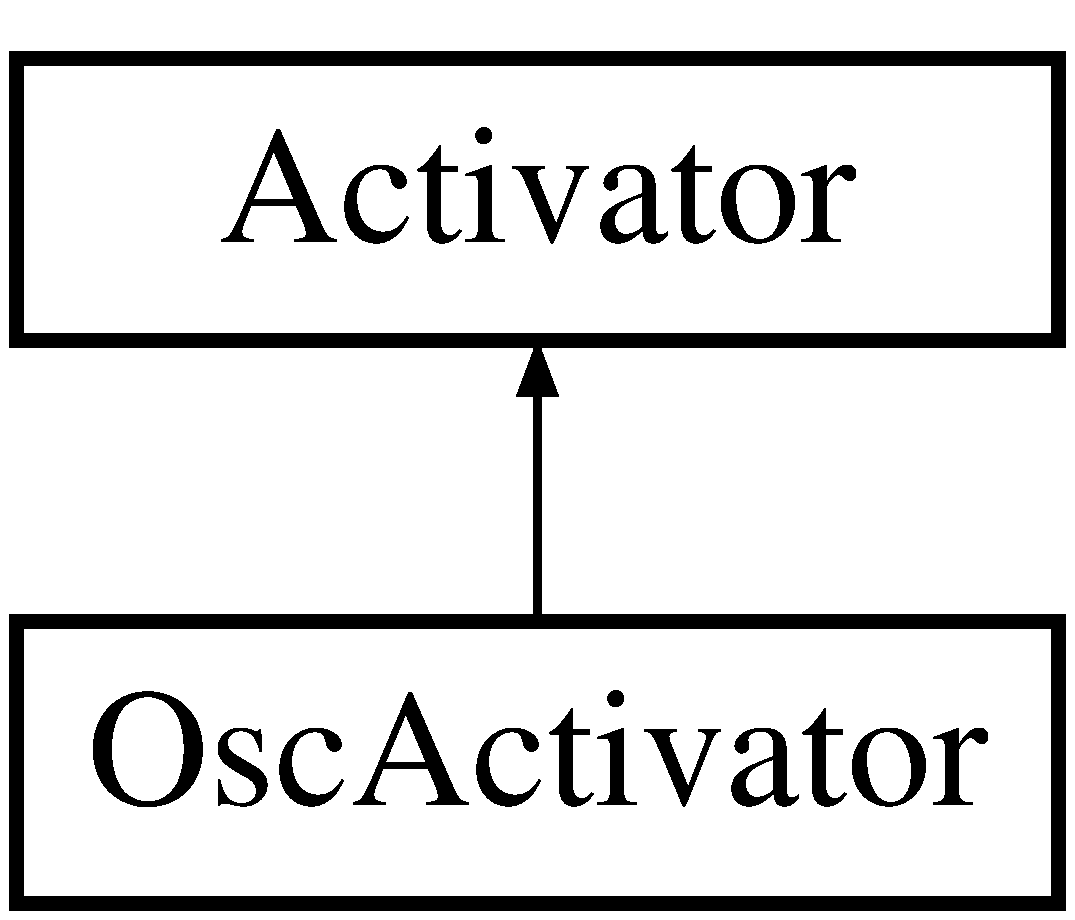
\includegraphics[height=2.000000cm]{classActivator}
\end{center}
\end{figure}
\subsection*{Public Member Functions}
\begin{DoxyCompactItemize}
\item 
virtual void {\bfseries callback} (float value)\hypertarget{classActivator_ace74b175ffcc2ad9cc03f15a0e713743}{}\label{classActivator_ace74b175ffcc2ad9cc03f15a0e713743}

\end{DoxyCompactItemize}


The documentation for this class was generated from the following files\+:\begin{DoxyCompactItemize}
\item 
include/Activator.\+h\item 
sequencer/Activator.\+cpp\end{DoxyCompactItemize}

\hypertarget{classunit_1_1AddTwoGen}{}\section{unit\+:\+:Add\+Two\+Gen Class Reference}
\label{classunit_1_1AddTwoGen}\index{unit\+::\+Add\+Two\+Gen@{unit\+::\+Add\+Two\+Gen}}


{\ttfamily \#include $<$Add\+Two\+Gen.\+h$>$}

Inheritance diagram for unit\+:\+:Add\+Two\+Gen\+:\begin{figure}[H]
\begin{center}
\leavevmode
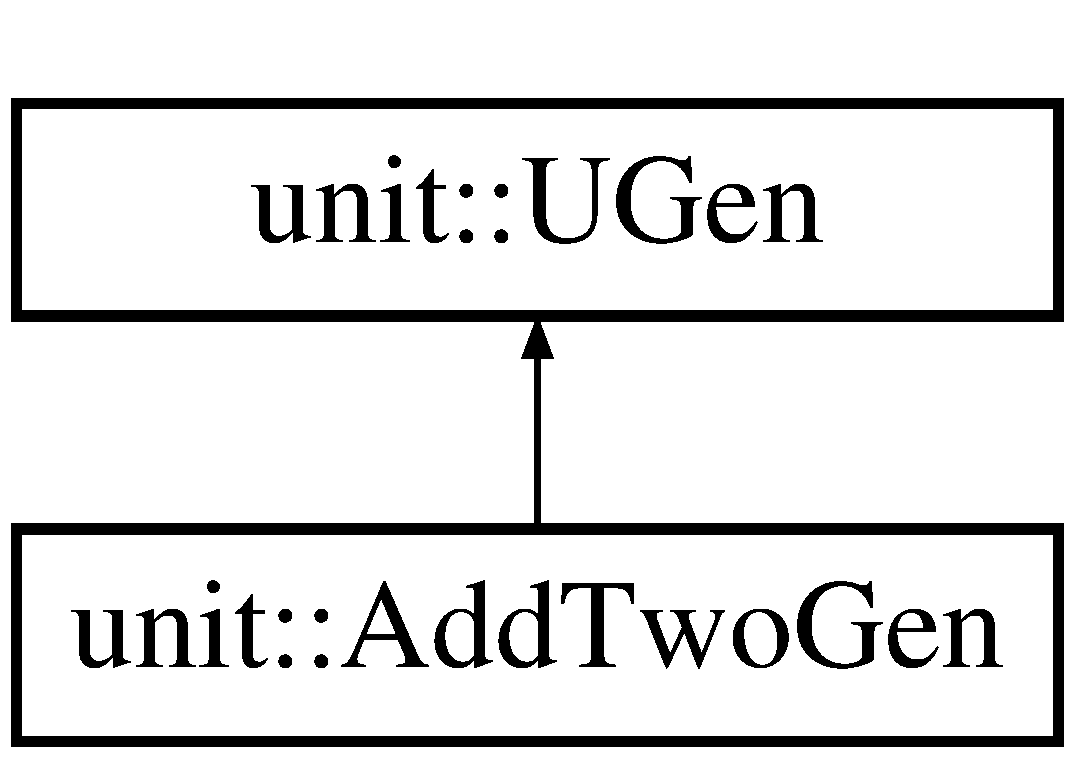
\includegraphics[height=2.000000cm]{classunit_1_1AddTwoGen}
\end{center}
\end{figure}
\subsection*{Public Member Functions}
\begin{DoxyCompactItemize}
\item 
{\bfseries Add\+Two\+Gen} (std\+::string name)\hypertarget{classunit_1_1AddTwoGen_a6feb4da948f12b37eb4502899b5a4311}{}\label{classunit_1_1AddTwoGen_a6feb4da948f12b37eb4502899b5a4311}

\item 
void {\bfseries control} (std\+::string port\+Name, float value)\hypertarget{classunit_1_1AddTwoGen_a5e0a82722566595b7284386a618ef3cb}{}\label{classunit_1_1AddTwoGen_a5e0a82722566595b7284386a618ef3cb}

\item 
float {\bfseries tick} ()\hypertarget{classunit_1_1AddTwoGen_a8e667f4f6c6849faef9f07a62e779d9a}{}\label{classunit_1_1AddTwoGen_a8e667f4f6c6849faef9f07a62e779d9a}

\end{DoxyCompactItemize}
\subsection*{Additional Inherited Members}


\subsection{Detailed Description}
\hyperlink{classunit_1_1AddTwoGen}{Add\+Two\+Gen} is calculating the arithmetic mean of \hyperlink{classPort}{Port} in1 and \hyperlink{classPort}{Port} in2. It provides a very basic two input mixing unit, adding together the Ports in1 and in2.

\begin{DoxyAuthor}{Author}
jtm 
\end{DoxyAuthor}
\begin{DoxySince}{Since}
04-\/2016 
\end{DoxySince}
\begin{DoxyVersion}{Version}
1.\+0 
\end{DoxyVersion}


The documentation for this class was generated from the following files\+:\begin{DoxyCompactItemize}
\item 
include/Add\+Two\+Gen.\+h\item 
unit/Add\+Two\+Gen.\+cpp\end{DoxyCompactItemize}

\hypertarget{classunit_1_1ADSR__NewGen}{}\section{unit\+:\+:A\+D\+S\+R\+\_\+\+New\+Gen Class Reference}
\label{classunit_1_1ADSR__NewGen}\index{unit\+::\+A\+D\+S\+R\+\_\+\+New\+Gen@{unit\+::\+A\+D\+S\+R\+\_\+\+New\+Gen}}
Inheritance diagram for unit\+:\+:A\+D\+S\+R\+\_\+\+New\+Gen\+:\begin{figure}[H]
\begin{center}
\leavevmode
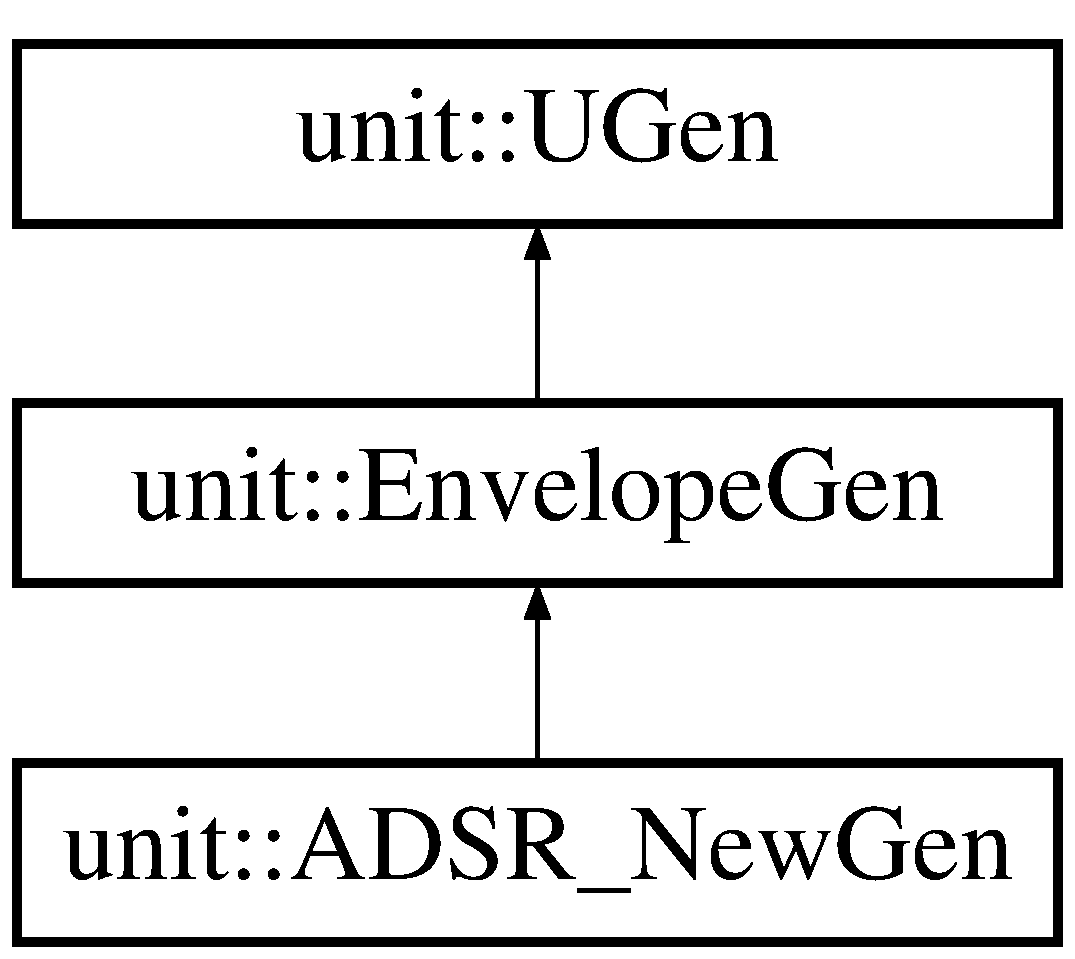
\includegraphics[height=3.000000cm]{classunit_1_1ADSR__NewGen}
\end{center}
\end{figure}
\subsection*{Public Member Functions}
\begin{DoxyCompactItemize}
\item 
{\bfseries A\+D\+S\+R\+\_\+\+New\+Gen} (std\+::string name)\hypertarget{classunit_1_1ADSR__NewGen_ac8dbe9f3fab627d291ed34996e97d73e}{}\label{classunit_1_1ADSR__NewGen_ac8dbe9f3fab627d291ed34996e97d73e}

\item 
void {\bfseries control} (std\+::string port\+Name, float value)\hypertarget{classunit_1_1ADSR__NewGen_ae5d3a6e3e2be04a470eeb30767e11a58}{}\label{classunit_1_1ADSR__NewGen_ae5d3a6e3e2be04a470eeb30767e11a58}

\item 
float {\bfseries tick} ()\hypertarget{classunit_1_1ADSR__NewGen_a9ec42e7edded490dbe69cbe93883b168}{}\label{classunit_1_1ADSR__NewGen_a9ec42e7edded490dbe69cbe93883b168}

\item 
void {\bfseries set\+Trigger} ()\hypertarget{classunit_1_1ADSR__NewGen_af3002642e550abcfe4be667d027670a9}{}\label{classunit_1_1ADSR__NewGen_af3002642e550abcfe4be667d027670a9}

\item 
void {\bfseries set\+Gate} (float value)\hypertarget{classunit_1_1ADSR__NewGen_a222a12be57cca522ece84deac512c330}{}\label{classunit_1_1ADSR__NewGen_a222a12be57cca522ece84deac512c330}

\item 
void {\bfseries set\+Attack} (float value)\hypertarget{classunit_1_1ADSR__NewGen_aa725e7a7c15ac05c643f3a9df9542c66}{}\label{classunit_1_1ADSR__NewGen_aa725e7a7c15ac05c643f3a9df9542c66}

\item 
void {\bfseries set\+Decay} (float value)\hypertarget{classunit_1_1ADSR__NewGen_aa43684929b80892b7d91ec75303fd00c}{}\label{classunit_1_1ADSR__NewGen_aa43684929b80892b7d91ec75303fd00c}

\item 
void {\bfseries set\+Sustain} (float value)\hypertarget{classunit_1_1ADSR__NewGen_a91036e95f48e88f71973dced76097563}{}\label{classunit_1_1ADSR__NewGen_a91036e95f48e88f71973dced76097563}

\item 
void {\bfseries set\+Release} (float value)\hypertarget{classunit_1_1ADSR__NewGen_af7e268918cef20f67514df7356f0fb15}{}\label{classunit_1_1ADSR__NewGen_af7e268918cef20f67514df7356f0fb15}

\end{DoxyCompactItemize}
\subsection*{Additional Inherited Members}


The documentation for this class was generated from the following files\+:\begin{DoxyCompactItemize}
\item 
unit/A\+D\+S\+R-\/\+New\+Gen.\+h\item 
unit/A\+D\+S\+R-\/\+New\+Gen.\+cpp\end{DoxyCompactItemize}

\hypertarget{classunit_1_1ADSRGen}{\section{unit\-:\-:A\-D\-S\-R\-Gen Class Reference}
\label{classunit_1_1ADSRGen}\index{unit\-::\-A\-D\-S\-R\-Gen@{unit\-::\-A\-D\-S\-R\-Gen}}
}
Inheritance diagram for unit\-:\-:A\-D\-S\-R\-Gen\-:\begin{figure}[H]
\begin{center}
\leavevmode
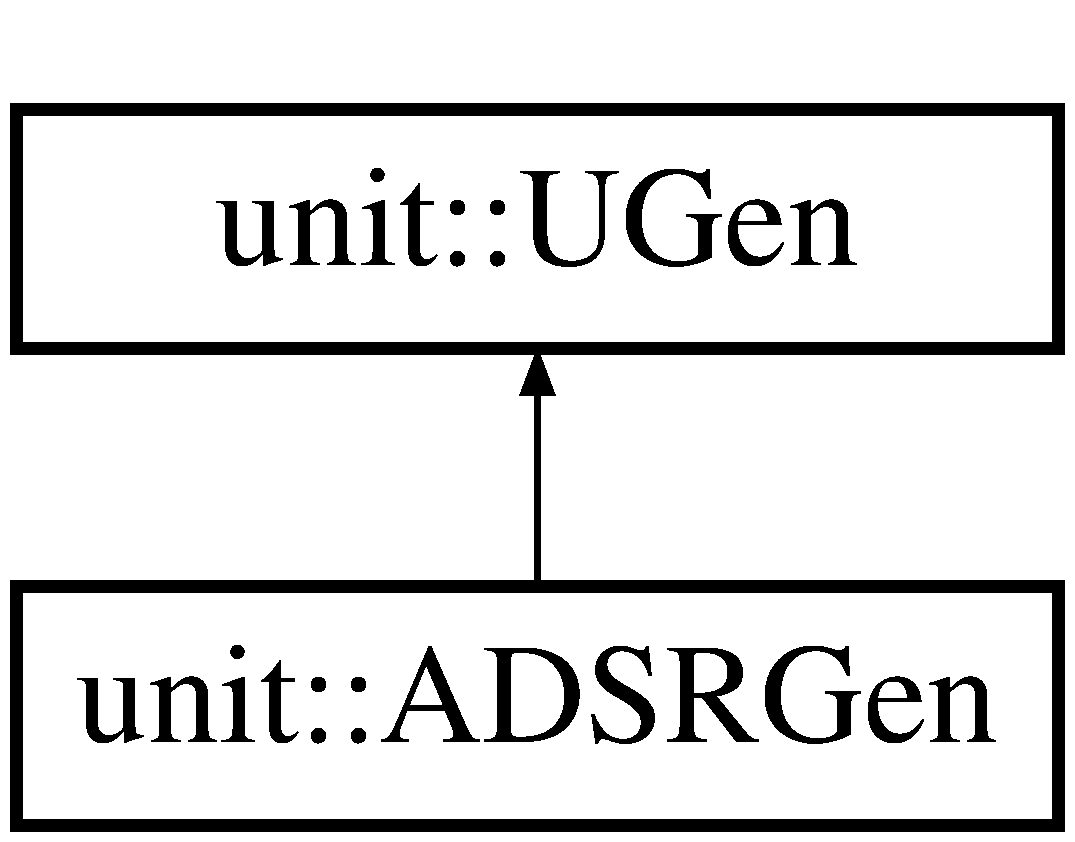
\includegraphics[height=3.000000cm]{classunit_1_1ADSRGen}
\end{center}
\end{figure}
\subsection*{Public Member Functions}
\begin{DoxyCompactItemize}
\item 
\hypertarget{classunit_1_1ADSRGen_a7e2d63eecbe51fc86a93697dd4d47964}{{\bfseries A\-D\-S\-R\-Gen} (std\-::string name)}\label{classunit_1_1ADSRGen_a7e2d63eecbe51fc86a93697dd4d47964}

\item 
\hypertarget{classunit_1_1ADSRGen_ac43bddd25b9a84f0ad6b299ed55f5133}{void {\bfseries control} (std\-::string port\-Name, float value)}\label{classunit_1_1ADSRGen_ac43bddd25b9a84f0ad6b299ed55f5133}

\item 
\hypertarget{classunit_1_1ADSRGen_a91a149fa5065d94dccec224b18710a24}{float {\bfseries tick} ()}\label{classunit_1_1ADSRGen_a91a149fa5065d94dccec224b18710a24}

\item 
\hypertarget{classunit_1_1ADSRGen_a8685be5cffea6ec29dc1ebdc44402f70}{void {\bfseries set\-Trigger} ()}\label{classunit_1_1ADSRGen_a8685be5cffea6ec29dc1ebdc44402f70}

\item 
\hypertarget{classunit_1_1ADSRGen_aee81e429433522eeb6362338fe15d551}{void {\bfseries set\-Gate} (float value)}\label{classunit_1_1ADSRGen_aee81e429433522eeb6362338fe15d551}

\item 
\hypertarget{classunit_1_1ADSRGen_a3a81f7181fa8b63f4ec5ff9da91cb8b3}{void {\bfseries set\-Attack} (float value)}\label{classunit_1_1ADSRGen_a3a81f7181fa8b63f4ec5ff9da91cb8b3}

\item 
\hypertarget{classunit_1_1ADSRGen_a14856bf0586881cbe088ab47918b7d72}{void {\bfseries set\-Decay} (float value)}\label{classunit_1_1ADSRGen_a14856bf0586881cbe088ab47918b7d72}

\item 
\hypertarget{classunit_1_1ADSRGen_a07fa6e650dc1ffdde91fc0721d4a8dc8}{void {\bfseries set\-Sustain} (float value)}\label{classunit_1_1ADSRGen_a07fa6e650dc1ffdde91fc0721d4a8dc8}

\item 
\hypertarget{classunit_1_1ADSRGen_a8c2a3e60dcae34d077b5983b1584de71}{void {\bfseries set\-Release} (float value)}\label{classunit_1_1ADSRGen_a8c2a3e60dcae34d077b5983b1584de71}

\end{DoxyCompactItemize}
\subsection*{Additional Inherited Members}


The documentation for this class was generated from the following files\-:\begin{DoxyCompactItemize}
\item 
include/A\-D\-S\-R\-Gen.\-h\item 
unit/A\-D\-S\-R\-Gen.\-cpp\end{DoxyCompactItemize}

\hypertarget{classADSRWorkshopSPU}{\section{A\-D\-S\-R\-Workshop\-S\-P\-U Class Reference}
\label{classADSRWorkshopSPU}\index{A\-D\-S\-R\-Workshop\-S\-P\-U@{A\-D\-S\-R\-Workshop\-S\-P\-U}}
}
Inheritance diagram for A\-D\-S\-R\-Workshop\-S\-P\-U\-:\begin{figure}[H]
\begin{center}
\leavevmode
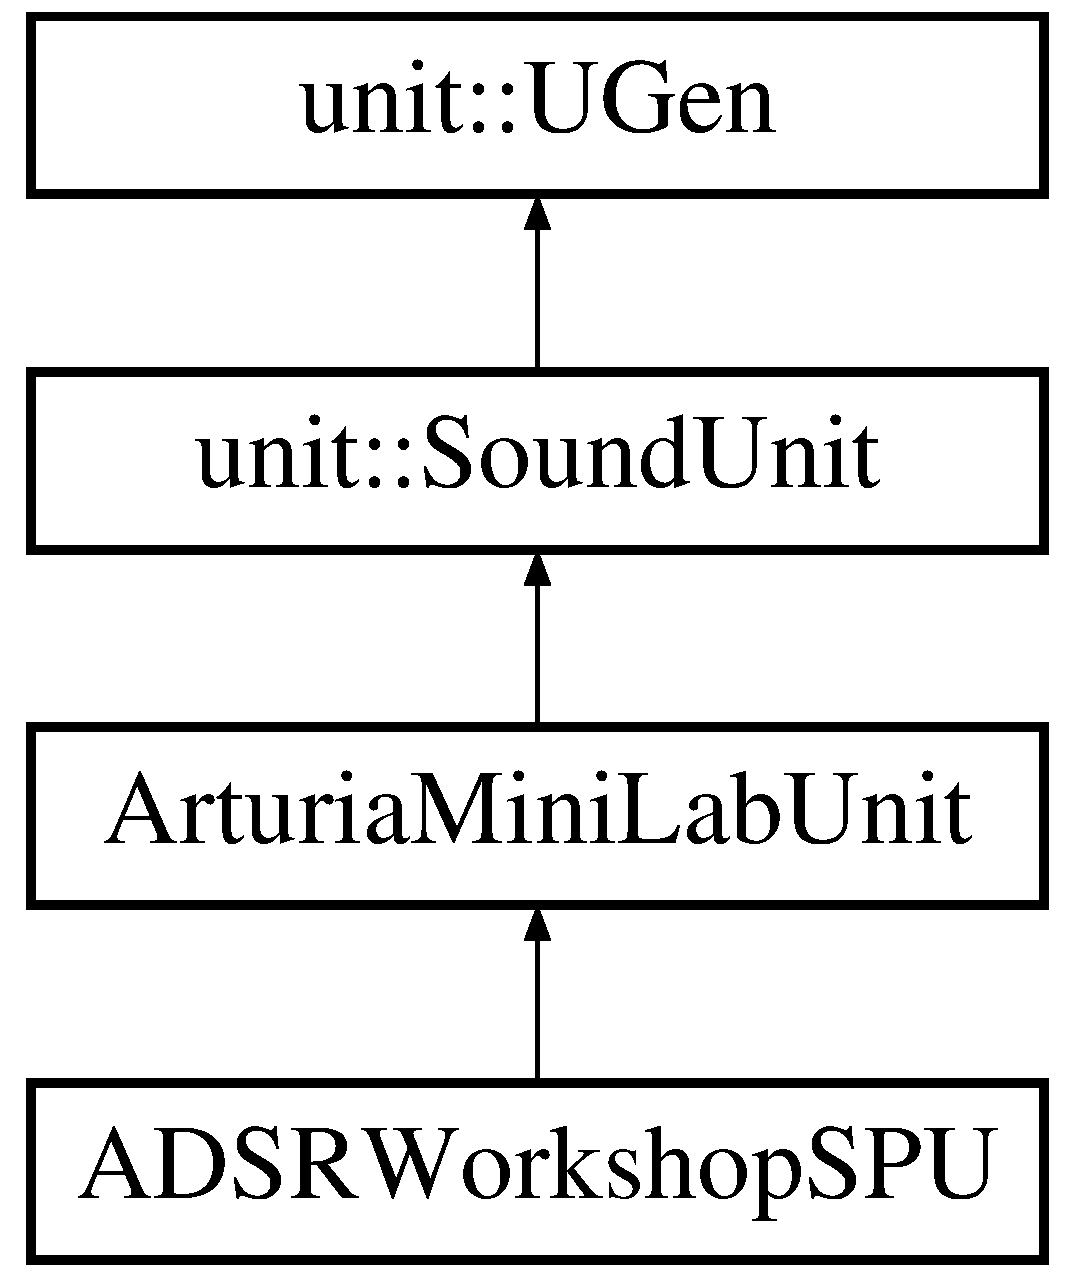
\includegraphics[height=4.000000cm]{classADSRWorkshopSPU}
\end{center}
\end{figure}
\subsection*{Public Member Functions}
\begin{DoxyCompactItemize}
\item 
\hypertarget{classADSRWorkshopSPU_a2140f477c0bdc9fac9b66a6c103bb126}{{\bfseries A\-D\-S\-R\-Workshop\-S\-P\-U} (std\-::string name)}\label{classADSRWorkshopSPU_a2140f477c0bdc9fac9b66a6c103bb126}

\item 
\hypertarget{classADSRWorkshopSPU_a8ec50457bbb3455b797f87cdb9988164}{float {\bfseries tick} ()}\label{classADSRWorkshopSPU_a8ec50457bbb3455b797f87cdb9988164}

\item 
\hypertarget{classADSRWorkshopSPU_af50b5a155375a444b9ebfe154b643409}{void {\bfseries control} (std\-::string port\-Name, float value)}\label{classADSRWorkshopSPU_af50b5a155375a444b9ebfe154b643409}

\item 
\hypertarget{classADSRWorkshopSPU_a961200f724c466c0dc0a0156dd01cbcc}{void {\bfseries set\-Trigger} ()}\label{classADSRWorkshopSPU_a961200f724c466c0dc0a0156dd01cbcc}

\item 
\hypertarget{classADSRWorkshopSPU_a51be23dcf951c1e752c218bf3c0be9bd}{void {\bfseries set\-Gate} (float value)}\label{classADSRWorkshopSPU_a51be23dcf951c1e752c218bf3c0be9bd}

\end{DoxyCompactItemize}
\subsection*{Additional Inherited Members}


The documentation for this class was generated from the following files\-:\begin{DoxyCompactItemize}
\item 
src/include/A\-D\-S\-R\-Workshop\-S\-P\-U.\-h\item 
src/spu/A\-D\-S\-R\-Workshop\-S\-P\-U.\-cpp\end{DoxyCompactItemize}

\hypertarget{classArturiaMiniLabUnit}{}\section{Arturia\+Mini\+Lab\+Unit Class Reference}
\label{classArturiaMiniLabUnit}\index{Arturia\+Mini\+Lab\+Unit@{Arturia\+Mini\+Lab\+Unit}}


{\ttfamily \#include $<$Arturia\+Mini\+Lab\+Unit.\+h$>$}

Inheritance diagram for Arturia\+Mini\+Lab\+Unit\+:\begin{figure}[H]
\begin{center}
\leavevmode
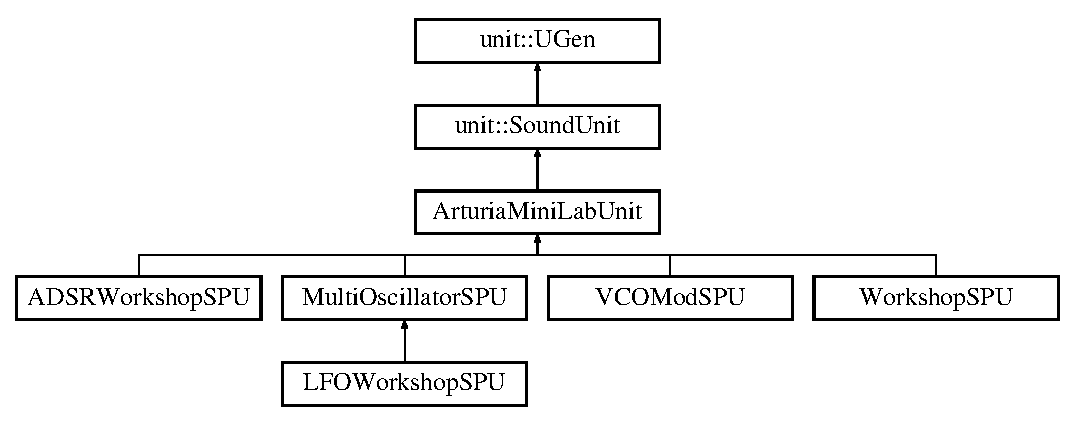
\includegraphics[height=5.000000cm]{classArturiaMiniLabUnit}
\end{center}
\end{figure}
\subsection*{Public Member Functions}
\begin{DoxyCompactItemize}
\item 
{\bfseries Arturia\+Mini\+Lab\+Unit} (std\+::string name)\hypertarget{classArturiaMiniLabUnit_aeb63b33d9631976240fd38d36935b44c}{}\label{classArturiaMiniLabUnit_aeb63b33d9631976240fd38d36935b44c}

\item 
void {\bfseries setup} ()\hypertarget{classArturiaMiniLabUnit_ae7590bc31683c4dc12b0a1396c53c6b4}{}\label{classArturiaMiniLabUnit_ae7590bc31683c4dc12b0a1396c53c6b4}

\item 
float {\bfseries tick} ()\hypertarget{classArturiaMiniLabUnit_a5d9365ac51fa7f46fdbd53c4f473bfcd}{}\label{classArturiaMiniLabUnit_a5d9365ac51fa7f46fdbd53c4f473bfcd}

\item 
void {\bfseries process\+Midi\+Message} (int type, int key, float value)\hypertarget{classArturiaMiniLabUnit_a0bb1d1b81bb3faf7ee141b941cf84457}{}\label{classArturiaMiniLabUnit_a0bb1d1b81bb3faf7ee141b941cf84457}

\item 
void {\bfseries process\+Control\+Message} (int type, int key, float value)\hypertarget{classArturiaMiniLabUnit_ad8f03d0e1bbe21f115f99c156c0f2d06}{}\label{classArturiaMiniLabUnit_ad8f03d0e1bbe21f115f99c156c0f2d06}

\end{DoxyCompactItemize}
\subsection*{Additional Inherited Members}


\subsection{Detailed Description}
\hyperlink{classArturiaMiniLabUnit}{Arturia\+Mini\+Lab\+Unit} provides an adapter to the Arturia Mini\+Lab controller. All keys, knobs, pads and sliders are mapped to control calls.

The Unit will later be replaced by a generic hardware abstraction unit, that loads the mapping information from a configuraiton file.

\begin{DoxyAuthor}{Author}
jtm, email\+:  \href{mailto:milde@hs-fulda.de}{\tt milde@hs-\/fulda.\+de} 
\end{DoxyAuthor}
\begin{DoxySince}{Since}
04-\/2016 
\end{DoxySince}
\begin{DoxyVersion}{Version}
1.\+0 
\end{DoxyVersion}


The documentation for this class was generated from the following files\+:\begin{DoxyCompactItemize}
\item 
include/Arturia\+Mini\+Lab\+Unit.\+h\item 
spu/Arturia\+Mini\+Lab\+Unit.\+cpp\end{DoxyCompactItemize}

\hypertarget{classCONFIG4CPP__NAMESPACE_1_1BufferedFileReader}{\section{C\-O\-N\-F\-I\-G4\-C\-P\-P\-\_\-\-N\-A\-M\-E\-S\-P\-A\-C\-E\-:\-:Buffered\-File\-Reader Class Reference}
\label{classCONFIG4CPP__NAMESPACE_1_1BufferedFileReader}\index{C\-O\-N\-F\-I\-G4\-C\-P\-P\-\_\-\-N\-A\-M\-E\-S\-P\-A\-C\-E\-::\-Buffered\-File\-Reader@{C\-O\-N\-F\-I\-G4\-C\-P\-P\-\_\-\-N\-A\-M\-E\-S\-P\-A\-C\-E\-::\-Buffered\-File\-Reader}}
}
\subsection*{Public Member Functions}
\begin{DoxyCompactItemize}
\item 
\hypertarget{classCONFIG4CPP__NAMESPACE_1_1BufferedFileReader_a339c2d89211e56a705f963eb67e8258a}{bool {\bfseries open} (const char $\ast$file\-Name)}\label{classCONFIG4CPP__NAMESPACE_1_1BufferedFileReader_a339c2d89211e56a705f963eb67e8258a}

\item 
\hypertarget{classCONFIG4CPP__NAMESPACE_1_1BufferedFileReader_ac2c7bdfc743c33aae63f2739112b50f4}{int {\bfseries get\-Char} ()}\label{classCONFIG4CPP__NAMESPACE_1_1BufferedFileReader_ac2c7bdfc743c33aae63f2739112b50f4}

\item 
\hypertarget{classCONFIG4CPP__NAMESPACE_1_1BufferedFileReader_a42aafc0d7e1403fa2cd86526faf198ec}{bool {\bfseries close} ()}\label{classCONFIG4CPP__NAMESPACE_1_1BufferedFileReader_a42aafc0d7e1403fa2cd86526faf198ec}

\end{DoxyCompactItemize}


The documentation for this class was generated from the following files\-:\begin{DoxyCompactItemize}
\item 
src/configuration/config4cpp/src/platform.\-h\item 
src/configuration/config4cpp/src/platform.\-cpp\end{DoxyCompactItemize}

\hypertarget{classCentralStore}{\section{Central\-Store Class Reference}
\label{classCentralStore}\index{Central\-Store@{Central\-Store}}
}
\subsection*{Public Member Functions}
\begin{DoxyCompactItemize}
\item 
\hypertarget{classCentralStore_ab809e0f4e90d4d8d1873a89f3da889b3}{void {\bfseries tick} ()}\label{classCentralStore_ab809e0f4e90d4d8d1873a89f3da889b3}

\item 
\hypertarget{classCentralStore_a100ae6ad2506d4962d23966e23a1c78e}{void {\bfseries clear} ()}\label{classCentralStore_a100ae6ad2506d4962d23966e23a1c78e}

\item 
\hypertarget{classCentralStore_a910470f5eec98b92b82a4cb2f1c5f386}{\hyperlink{classosc_1_1MessageData}{osc\-::\-Message\-Data} $\ast$ {\bfseries get\-Midi\-Data} ()}\label{classCentralStore_a910470f5eec98b92b82a4cb2f1c5f386}

\item 
\hypertarget{classCentralStore_a3faaea58a012d25efaa710fa3d1942b7}{\hyperlink{classosc_1_1MessageData}{osc\-::\-Message\-Data} $\ast$ {\bfseries get\-Control\-Data} ()}\label{classCentralStore_a3faaea58a012d25efaa710fa3d1942b7}

\end{DoxyCompactItemize}
\subsection*{Public Attributes}
\begin{DoxyCompactItemize}
\item 
\hypertarget{classCentralStore_a6f0c4050f0983924bbad8c631746f8b7}{\hyperlink{structTickData}{Tick\-Data} {\bfseries tick\-Data}}\label{classCentralStore_a6f0c4050f0983924bbad8c631746f8b7}

\end{DoxyCompactItemize}


The documentation for this class was generated from the following files\-:\begin{DoxyCompactItemize}
\item 
src/include/Central\-Store.\-h\item 
src/store/Central\-Store.\-cpp\end{DoxyCompactItemize}

\hypertarget{classCONFIG4CPP__NAMESPACE_1_1Config2Cpp}{\section{C\-O\-N\-F\-I\-G4\-C\-P\-P\-\_\-\-N\-A\-M\-E\-S\-P\-A\-C\-E\-:\-:Config2\-Cpp Class Reference}
\label{classCONFIG4CPP__NAMESPACE_1_1Config2Cpp}\index{C\-O\-N\-F\-I\-G4\-C\-P\-P\-\_\-\-N\-A\-M\-E\-S\-P\-A\-C\-E\-::\-Config2\-Cpp@{C\-O\-N\-F\-I\-G4\-C\-P\-P\-\_\-\-N\-A\-M\-E\-S\-P\-A\-C\-E\-::\-Config2\-Cpp}}
}
\subsection*{Public Member Functions}
\begin{DoxyCompactItemize}
\item 
\hypertarget{classCONFIG4CPP__NAMESPACE_1_1Config2Cpp_abcfb558647a328e709fd184feb85abd3}{{\bfseries Config2\-Cpp} (const char $\ast$prog\-Name)}\label{classCONFIG4CPP__NAMESPACE_1_1Config2Cpp_abcfb558647a328e709fd184feb85abd3}

\item 
\hypertarget{classCONFIG4CPP__NAMESPACE_1_1Config2Cpp_ad083a2e806c5ff95b75b2bf520b3997a}{bool {\bfseries parse\-Cmd\-Line\-Args} (int argc, char $\ast$$\ast$argv)}\label{classCONFIG4CPP__NAMESPACE_1_1Config2Cpp_ad083a2e806c5ff95b75b2bf520b3997a}

\item 
\hypertarget{classCONFIG4CPP__NAMESPACE_1_1Config2Cpp_a9c84ad99a97b335e701f2b4bb7479c90}{bool {\bfseries generate\-Files} (const char $\ast$const $\ast$schema, int schema\-Size)}\label{classCONFIG4CPP__NAMESPACE_1_1Config2Cpp_a9c84ad99a97b335e701f2b4bb7479c90}

\item 
\hypertarget{classCONFIG4CPP__NAMESPACE_1_1Config2Cpp_a9a51831d179cd72f467bb8ef91ee0281}{const char $\ast$ {\bfseries cfg\-File\-Name} ()}\label{classCONFIG4CPP__NAMESPACE_1_1Config2Cpp_a9a51831d179cd72f467bb8ef91ee0281}

\item 
\hypertarget{classCONFIG4CPP__NAMESPACE_1_1Config2Cpp_a98814e664226758fc213b8befd81e21d}{const char $\ast$ {\bfseries schema\-Override\-Cfg} ()}\label{classCONFIG4CPP__NAMESPACE_1_1Config2Cpp_a98814e664226758fc213b8befd81e21d}

\item 
\hypertarget{classCONFIG4CPP__NAMESPACE_1_1Config2Cpp_aedf47578fff7433024dac61ef374c0ec}{const char $\ast$ {\bfseries schema\-Override\-Scope} ()}\label{classCONFIG4CPP__NAMESPACE_1_1Config2Cpp_aedf47578fff7433024dac61ef374c0ec}

\item 
\hypertarget{classCONFIG4CPP__NAMESPACE_1_1Config2Cpp_a28836cb450289ac0c37965ef581fb98c}{const char $\ast$ {\bfseries class\-Name} ()}\label{classCONFIG4CPP__NAMESPACE_1_1Config2Cpp_a28836cb450289ac0c37965ef581fb98c}

\item 
\hypertarget{classCONFIG4CPP__NAMESPACE_1_1Config2Cpp_a9a569781f751ec8cbf2dc58472143a73}{const char $\ast$ {\bfseries cpp\-Ext} ()}\label{classCONFIG4CPP__NAMESPACE_1_1Config2Cpp_a9a569781f751ec8cbf2dc58472143a73}

\item 
\hypertarget{classCONFIG4CPP__NAMESPACE_1_1Config2Cpp_adb9c986ec921522aa48a1b42ec04b675}{const char $\ast$ {\bfseries h\-Ext} ()}\label{classCONFIG4CPP__NAMESPACE_1_1Config2Cpp_adb9c986ec921522aa48a1b42ec04b675}

\item 
\hypertarget{classCONFIG4CPP__NAMESPACE_1_1Config2Cpp_aac349fdbbf8a879a30c7a29575d65cfc}{bool {\bfseries want\-Schema} ()}\label{classCONFIG4CPP__NAMESPACE_1_1Config2Cpp_aac349fdbbf8a879a30c7a29575d65cfc}

\end{DoxyCompactItemize}


The documentation for this class was generated from the following files\-:\begin{DoxyCompactItemize}
\item 
src/configuration/config4cpp/src/Config2\-Cpp.\-h\item 
src/configuration/config4cpp/src/Config2\-Cpp.\-cpp\end{DoxyCompactItemize}

\hypertarget{classCONFIG4CPP__NAMESPACE_1_1ConfigItem}{\section{C\-O\-N\-F\-I\-G4\-C\-P\-P\-\_\-\-N\-A\-M\-E\-S\-P\-A\-C\-E\-:\-:Config\-Item Class Reference}
\label{classCONFIG4CPP__NAMESPACE_1_1ConfigItem}\index{C\-O\-N\-F\-I\-G4\-C\-P\-P\-\_\-\-N\-A\-M\-E\-S\-P\-A\-C\-E\-::\-Config\-Item@{C\-O\-N\-F\-I\-G4\-C\-P\-P\-\_\-\-N\-A\-M\-E\-S\-P\-A\-C\-E\-::\-Config\-Item}}
}
\subsection*{Public Member Functions}
\begin{DoxyCompactItemize}
\item 
\hypertarget{classCONFIG4CPP__NAMESPACE_1_1ConfigItem_af9551942ab375a3cf60df63589a45c87}{{\bfseries Config\-Item} (const char $\ast$name, const char $\ast$str)}\label{classCONFIG4CPP__NAMESPACE_1_1ConfigItem_af9551942ab375a3cf60df63589a45c87}

\item 
\hypertarget{classCONFIG4CPP__NAMESPACE_1_1ConfigItem_a688097c07bf2e67d1888c0368ecadae9}{{\bfseries Config\-Item} (const char $\ast$name, const \hyperlink{classCONFIG4CPP__NAMESPACE_1_1StringVector}{String\-Vector} \&list)}\label{classCONFIG4CPP__NAMESPACE_1_1ConfigItem_a688097c07bf2e67d1888c0368ecadae9}

\item 
\hypertarget{classCONFIG4CPP__NAMESPACE_1_1ConfigItem_a0a144e78555d2373e74a13e49006f1eb}{{\bfseries Config\-Item} (const char $\ast$name, const char $\ast$$\ast$array, int size)}\label{classCONFIG4CPP__NAMESPACE_1_1ConfigItem_a0a144e78555d2373e74a13e49006f1eb}

\item 
\hypertarget{classCONFIG4CPP__NAMESPACE_1_1ConfigItem_aaa0335d449d3cd8784e6b5f4f1754e4d}{{\bfseries Config\-Item} (const char $\ast$name, \hyperlink{classCONFIG4CPP__NAMESPACE_1_1ConfigScope}{Config\-Scope} $\ast$scope)}\label{classCONFIG4CPP__NAMESPACE_1_1ConfigItem_aaa0335d449d3cd8784e6b5f4f1754e4d}

\item 
\hypertarget{classCONFIG4CPP__NAMESPACE_1_1ConfigItem_aa4b7f08baac4a1ebb3a476f3dfd508c5}{Configuration\-::\-Type {\bfseries type} ()}\label{classCONFIG4CPP__NAMESPACE_1_1ConfigItem_aa4b7f08baac4a1ebb3a476f3dfd508c5}

\item 
\hypertarget{classCONFIG4CPP__NAMESPACE_1_1ConfigItem_a51d6a67ef249db10098450112839d73e}{const char $\ast$ {\bfseries name} () const }\label{classCONFIG4CPP__NAMESPACE_1_1ConfigItem_a51d6a67ef249db10098450112839d73e}

\item 
\hypertarget{classCONFIG4CPP__NAMESPACE_1_1ConfigItem_a6e248e3f61c53f81cc0e3fd4a703e690}{const char $\ast$ {\bfseries string\-Val} () const }\label{classCONFIG4CPP__NAMESPACE_1_1ConfigItem_a6e248e3f61c53f81cc0e3fd4a703e690}

\item 
\hypertarget{classCONFIG4CPP__NAMESPACE_1_1ConfigItem_a6f593cc48d18cd1ea52d66aacec47e2a}{\hyperlink{classCONFIG4CPP__NAMESPACE_1_1StringVector}{String\-Vector} \& {\bfseries list\-Val} () const }\label{classCONFIG4CPP__NAMESPACE_1_1ConfigItem_a6f593cc48d18cd1ea52d66aacec47e2a}

\item 
\hypertarget{classCONFIG4CPP__NAMESPACE_1_1ConfigItem_a337fb53482b221265adfde75fb350840}{\hyperlink{classCONFIG4CPP__NAMESPACE_1_1ConfigScope}{Config\-Scope} $\ast$ {\bfseries scope\-Val} () const }\label{classCONFIG4CPP__NAMESPACE_1_1ConfigItem_a337fb53482b221265adfde75fb350840}

\item 
\hypertarget{classCONFIG4CPP__NAMESPACE_1_1ConfigItem_a14361b26d97fde53038ec7b872449e2e}{void {\bfseries dump} (\hyperlink{classCONFIG4CPP__NAMESPACE_1_1StringBuffer}{String\-Buffer} \&buf, const char $\ast$name, bool want\-Expanded\-Uid\-Names, int indent\-Level=0) const }\label{classCONFIG4CPP__NAMESPACE_1_1ConfigItem_a14361b26d97fde53038ec7b872449e2e}

\end{DoxyCompactItemize}
\subsection*{Protected Attributes}
\begin{DoxyCompactItemize}
\item 
\hypertarget{classCONFIG4CPP__NAMESPACE_1_1ConfigItem_a97732e21abaa53cc86c055adcb9c7bc2}{Configuration\-::\-Type {\bfseries m\-\_\-type}}\label{classCONFIG4CPP__NAMESPACE_1_1ConfigItem_a97732e21abaa53cc86c055adcb9c7bc2}

\item 
\hypertarget{classCONFIG4CPP__NAMESPACE_1_1ConfigItem_a6cad122109711410fc6e1c4146dd1ec2}{char $\ast$ {\bfseries m\-\_\-name}}\label{classCONFIG4CPP__NAMESPACE_1_1ConfigItem_a6cad122109711410fc6e1c4146dd1ec2}

\item 
\hypertarget{classCONFIG4CPP__NAMESPACE_1_1ConfigItem_a6b54a9239321798beff068d52be82894}{char $\ast$ {\bfseries m\-\_\-string\-Val}}\label{classCONFIG4CPP__NAMESPACE_1_1ConfigItem_a6b54a9239321798beff068d52be82894}

\item 
\hypertarget{classCONFIG4CPP__NAMESPACE_1_1ConfigItem_a2f7d188fc4d49331eae74681a2b85732}{\hyperlink{classCONFIG4CPP__NAMESPACE_1_1StringVector}{String\-Vector} $\ast$ {\bfseries m\-\_\-list\-Val}}\label{classCONFIG4CPP__NAMESPACE_1_1ConfigItem_a2f7d188fc4d49331eae74681a2b85732}

\item 
\hypertarget{classCONFIG4CPP__NAMESPACE_1_1ConfigItem_afc25eec1fdb47acc47aaefcd69b0ebf6}{\hyperlink{classCONFIG4CPP__NAMESPACE_1_1ConfigScope}{Config\-Scope} $\ast$ {\bfseries m\-\_\-scope}}\label{classCONFIG4CPP__NAMESPACE_1_1ConfigItem_afc25eec1fdb47acc47aaefcd69b0ebf6}

\end{DoxyCompactItemize}


The documentation for this class was generated from the following files\-:\begin{DoxyCompactItemize}
\item 
src/configuration/config4cpp/src/Config\-Item.\-h\item 
src/configuration/config4cpp/src/Config\-Item.\-cpp\end{DoxyCompactItemize}

\hypertarget{classCONFIG4CPP__NAMESPACE_1_1ConfigLex}{\section{C\-O\-N\-F\-I\-G4\-C\-P\-P\-\_\-\-N\-A\-M\-E\-S\-P\-A\-C\-E\-:\-:Config\-Lex Class Reference}
\label{classCONFIG4CPP__NAMESPACE_1_1ConfigLex}\index{C\-O\-N\-F\-I\-G4\-C\-P\-P\-\_\-\-N\-A\-M\-E\-S\-P\-A\-C\-E\-::\-Config\-Lex@{C\-O\-N\-F\-I\-G4\-C\-P\-P\-\_\-\-N\-A\-M\-E\-S\-P\-A\-C\-E\-::\-Config\-Lex}}
}
Inheritance diagram for C\-O\-N\-F\-I\-G4\-C\-P\-P\-\_\-\-N\-A\-M\-E\-S\-P\-A\-C\-E\-:\-:Config\-Lex\-:\begin{figure}[H]
\begin{center}
\leavevmode
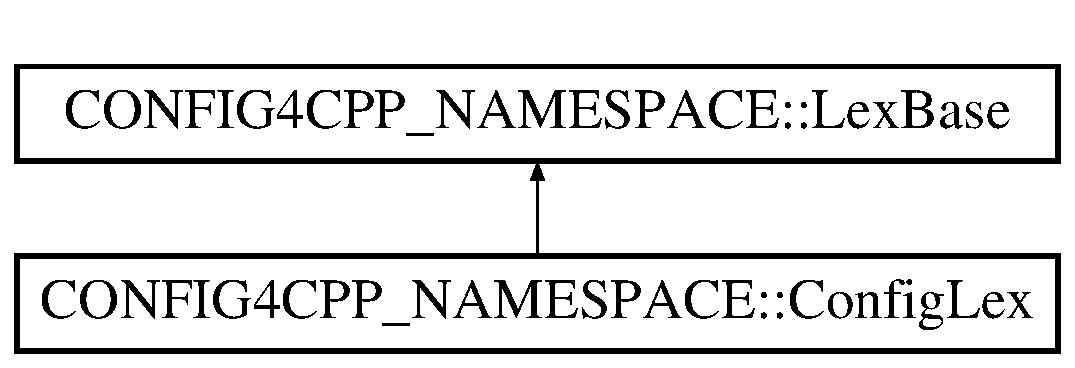
\includegraphics[height=2.000000cm]{classCONFIG4CPP__NAMESPACE_1_1ConfigLex}
\end{center}
\end{figure}
\subsection*{Public Types}
\begin{DoxyCompactItemize}
\item 
enum {\bfseries Config\-Lex\-Symbols} \{ \\*
{\bfseries L\-E\-X\-\_\-\-C\-O\-P\-Y\-\_\-\-F\-R\-O\-M\-\_\-\-S\-Y\-M} = 101, 
{\bfseries L\-E\-X\-\_\-\-E\-L\-S\-E\-\_\-\-S\-Y\-M} = 102, 
{\bfseries L\-E\-X\-\_\-\-E\-L\-S\-E\-\_\-\-I\-F\-\_\-\-S\-Y\-M} = 103, 
{\bfseries L\-E\-X\-\_\-\-E\-R\-R\-O\-R\-\_\-\-S\-Y\-M} = 104, 
\\*
{\bfseries L\-E\-X\-\_\-\-I\-F\-\_\-\-S\-Y\-M} = 105, 
{\bfseries L\-E\-X\-\_\-\-I\-F\-\_\-\-E\-X\-I\-S\-T\-S\-\_\-\-S\-Y\-M} = 106, 
{\bfseries L\-E\-X\-\_\-\-I\-N\-\_\-\-S\-Y\-M} = 107, 
{\bfseries L\-E\-X\-\_\-\-I\-N\-C\-L\-U\-D\-E\-\_\-\-S\-Y\-M} = 108, 
\\*
{\bfseries L\-E\-X\-\_\-\-M\-A\-T\-C\-H\-E\-S\-\_\-\-S\-Y\-M} = 109, 
{\bfseries L\-E\-X\-\_\-\-R\-E\-M\-O\-V\-E\-\_\-\-S\-Y\-M} = 110, 
{\bfseries L\-E\-X\-\_\-\-F\-U\-N\-C\-\_\-\-C\-O\-N\-F\-I\-G\-\_\-\-F\-I\-L\-E\-\_\-\-S\-Y\-M} = 201, 
{\bfseries L\-E\-X\-\_\-\-F\-U\-N\-C\-\_\-\-C\-O\-N\-F\-I\-G\-\_\-\-T\-Y\-P\-E\-\_\-\-S\-Y\-M} = 202, 
\\*
{\bfseries L\-E\-X\-\_\-\-F\-U\-N\-C\-\_\-\-E\-X\-E\-C\-\_\-\-S\-Y\-M} = 203, 
{\bfseries L\-E\-X\-\_\-\-F\-U\-N\-C\-\_\-\-F\-I\-L\-E\-\_\-\-T\-O\-\_\-\-D\-I\-R\-\_\-\-S\-Y\-M} = 204, 
{\bfseries L\-E\-X\-\_\-\-F\-U\-N\-C\-\_\-\-G\-E\-T\-E\-N\-V\-\_\-\-S\-Y\-M} = 205, 
{\bfseries L\-E\-X\-\_\-\-F\-U\-N\-C\-\_\-\-I\-S\-\_\-\-F\-I\-L\-E\-\_\-\-R\-E\-A\-D\-A\-B\-L\-E\-\_\-\-S\-Y\-M} = 206, 
\\*
{\bfseries L\-E\-X\-\_\-\-F\-U\-N\-C\-\_\-\-J\-O\-I\-N\-\_\-\-S\-Y\-M} = 207, 
{\bfseries L\-E\-X\-\_\-\-F\-U\-N\-C\-\_\-\-O\-S\-\_\-\-D\-I\-R\-\_\-\-S\-E\-P\-\_\-\-S\-Y\-M} = 208, 
{\bfseries L\-E\-X\-\_\-\-F\-U\-N\-C\-\_\-\-O\-S\-\_\-\-P\-A\-T\-H\-\_\-\-S\-E\-P\-\_\-\-S\-Y\-M} = 209, 
{\bfseries L\-E\-X\-\_\-\-F\-U\-N\-C\-\_\-\-O\-S\-\_\-\-T\-Y\-P\-E\-\_\-\-S\-Y\-M} = 210, 
\\*
{\bfseries L\-E\-X\-\_\-\-F\-U\-N\-C\-\_\-\-R\-E\-A\-D\-\_\-\-F\-I\-L\-E\-\_\-\-S\-Y\-M} = 211, 
{\bfseries L\-E\-X\-\_\-\-F\-U\-N\-C\-\_\-\-R\-E\-P\-L\-A\-C\-E\-\_\-\-S\-Y\-M} = 212, 
{\bfseries L\-E\-X\-\_\-\-F\-U\-N\-C\-\_\-\-S\-I\-B\-L\-I\-N\-G\-\_\-\-S\-C\-O\-P\-E\-\_\-\-S\-Y\-M} = 213, 
{\bfseries L\-E\-X\-\_\-\-F\-U\-N\-C\-\_\-\-S\-P\-L\-I\-T\-\_\-\-S\-Y\-M} = 214
 \}
\end{DoxyCompactItemize}
\subsection*{Public Member Functions}
\begin{DoxyCompactItemize}
\item 
\hypertarget{classCONFIG4CPP__NAMESPACE_1_1ConfigLex_a25fa2137da6a6d495d4a9c20100e44e8}{{\bfseries Config\-Lex} (Configuration\-::\-Source\-Type source\-Type, const char $\ast$source, \hyperlink{classCONFIG4CPP__NAMESPACE_1_1UidIdentifierProcessor}{Uid\-Identifier\-Processor} $\ast$uid\-Identifier\-Processor)  throw (\-Configuration\-Exception)}\label{classCONFIG4CPP__NAMESPACE_1_1ConfigLex_a25fa2137da6a6d495d4a9c20100e44e8}

\end{DoxyCompactItemize}
\subsection*{Additional Inherited Members}


The documentation for this class was generated from the following files\-:\begin{DoxyCompactItemize}
\item 
src/configuration/config4cpp/src/Config\-Lex.\-h\item 
src/configuration/config4cpp/src/Config\-Lex.\-cpp\end{DoxyCompactItemize}

\hypertarget{classCONFIG4CPP__NAMESPACE_1_1ConfigParser}{\section{C\-O\-N\-F\-I\-G4\-C\-P\-P\-\_\-\-N\-A\-M\-E\-S\-P\-A\-C\-E\-:\-:Config\-Parser Class Reference}
\label{classCONFIG4CPP__NAMESPACE_1_1ConfigParser}\index{C\-O\-N\-F\-I\-G4\-C\-P\-P\-\_\-\-N\-A\-M\-E\-S\-P\-A\-C\-E\-::\-Config\-Parser@{C\-O\-N\-F\-I\-G4\-C\-P\-P\-\_\-\-N\-A\-M\-E\-S\-P\-A\-C\-E\-::\-Config\-Parser}}
}
\subsection*{Public Member Functions}
\begin{DoxyCompactItemize}
\item 
\hypertarget{classCONFIG4CPP__NAMESPACE_1_1ConfigParser_a81b932edd6cd656d40f70cd9509777e2}{{\bfseries Config\-Parser} (Configuration\-::\-Source\-Type source\-Type, const char $\ast$source, const char $\ast$trusted\-Cmd\-Line, const char $\ast$source\-Description, \hyperlink{classCONFIG4CPP__NAMESPACE_1_1ConfigurationImpl}{Configuration\-Impl} $\ast$config, bool if\-Exists\-Is\-Specified=false)  throw (\-Configuration\-Exception)}\label{classCONFIG4CPP__NAMESPACE_1_1ConfigParser_a81b932edd6cd656d40f70cd9509777e2}

\end{DoxyCompactItemize}
\subsection*{Protected Member Functions}
\begin{DoxyCompactItemize}
\item 
\hypertarget{classCONFIG4CPP__NAMESPACE_1_1ConfigParser_af5a88acec6fae91a5fcb427e9d554358}{void {\bfseries parse\-Stmt\-List} ()}\label{classCONFIG4CPP__NAMESPACE_1_1ConfigParser_af5a88acec6fae91a5fcb427e9d554358}

\item 
\hypertarget{classCONFIG4CPP__NAMESPACE_1_1ConfigParser_ab383c065f81d9cfc58746f116b8ff90a}{void {\bfseries parse\-Stmt} ()}\label{classCONFIG4CPP__NAMESPACE_1_1ConfigParser_ab383c065f81d9cfc58746f116b8ff90a}

\item 
\hypertarget{classCONFIG4CPP__NAMESPACE_1_1ConfigParser_a2ce3ce02a7ea8d8e0879010c75e03652}{void {\bfseries parse\-Include\-Stmt} ()}\label{classCONFIG4CPP__NAMESPACE_1_1ConfigParser_a2ce3ce02a7ea8d8e0879010c75e03652}

\item 
\hypertarget{classCONFIG4CPP__NAMESPACE_1_1ConfigParser_a5166490f104d27861c8cdb50a707bc99}{void {\bfseries parse\-Copy\-Stmt} ()}\label{classCONFIG4CPP__NAMESPACE_1_1ConfigParser_a5166490f104d27861c8cdb50a707bc99}

\item 
\hypertarget{classCONFIG4CPP__NAMESPACE_1_1ConfigParser_a1a3a120168949e5063444055bdd469d6}{void {\bfseries parse\-Remove\-Stmt} ()}\label{classCONFIG4CPP__NAMESPACE_1_1ConfigParser_a1a3a120168949e5063444055bdd469d6}

\item 
\hypertarget{classCONFIG4CPP__NAMESPACE_1_1ConfigParser_a61ae1ac2164d0472eeb752ad380c6e6c}{void {\bfseries parse\-Error\-Stmt} ()}\label{classCONFIG4CPP__NAMESPACE_1_1ConfigParser_a61ae1ac2164d0472eeb752ad380c6e6c}

\item 
\hypertarget{classCONFIG4CPP__NAMESPACE_1_1ConfigParser_a6e7f827d10772dfd7f1fcc3f1b9bdded}{void {\bfseries parse\-If\-Stmt} ()}\label{classCONFIG4CPP__NAMESPACE_1_1ConfigParser_a6e7f827d10772dfd7f1fcc3f1b9bdded}

\item 
\hypertarget{classCONFIG4CPP__NAMESPACE_1_1ConfigParser_aa26b77130b24a00061163478fcc10d28}{void {\bfseries skip\-To\-Closing\-Brace} ()}\label{classCONFIG4CPP__NAMESPACE_1_1ConfigParser_aa26b77130b24a00061163478fcc10d28}

\item 
\hypertarget{classCONFIG4CPP__NAMESPACE_1_1ConfigParser_a3f8779c96cc188c9665a180d62c50350}{bool {\bfseries parse\-Condition} ()}\label{classCONFIG4CPP__NAMESPACE_1_1ConfigParser_a3f8779c96cc188c9665a180d62c50350}

\item 
\hypertarget{classCONFIG4CPP__NAMESPACE_1_1ConfigParser_a9a957643b9bc9f9d7dfd32e6cbaef88d}{bool {\bfseries parse\-Or\-Condition} ()}\label{classCONFIG4CPP__NAMESPACE_1_1ConfigParser_a9a957643b9bc9f9d7dfd32e6cbaef88d}

\item 
\hypertarget{classCONFIG4CPP__NAMESPACE_1_1ConfigParser_ae9db19b13ea66f280fcd12e81bb09378}{bool {\bfseries parse\-And\-Condition} ()}\label{classCONFIG4CPP__NAMESPACE_1_1ConfigParser_ae9db19b13ea66f280fcd12e81bb09378}

\item 
\hypertarget{classCONFIG4CPP__NAMESPACE_1_1ConfigParser_ad1f02197a52ffe992cf140bddff335ca}{bool {\bfseries parse\-Terminal\-Condition} ()}\label{classCONFIG4CPP__NAMESPACE_1_1ConfigParser_ad1f02197a52ffe992cf140bddff335ca}

\item 
\hypertarget{classCONFIG4CPP__NAMESPACE_1_1ConfigParser_a4377ccf82778184d5c9795fc35ba883c}{void {\bfseries parse\-Scope} (\hyperlink{classCONFIG4CPP__NAMESPACE_1_1LexToken}{Lex\-Token} \&scope\-Name)}\label{classCONFIG4CPP__NAMESPACE_1_1ConfigParser_a4377ccf82778184d5c9795fc35ba883c}

\item 
\hypertarget{classCONFIG4CPP__NAMESPACE_1_1ConfigParser_a6f75e8eb8c30bb26d41da9044e22aefd}{void {\bfseries parse\-Rhs\-Assign\-Stmt} (\hyperlink{classCONFIG4CPP__NAMESPACE_1_1LexToken}{Lex\-Token} \&var\-Name, short assignment\-Type)}\label{classCONFIG4CPP__NAMESPACE_1_1ConfigParser_a6f75e8eb8c30bb26d41da9044e22aefd}

\item 
\hypertarget{classCONFIG4CPP__NAMESPACE_1_1ConfigParser_a65edbff9a96b90e1726f7e52c84ab9ff}{void {\bfseries parse\-String\-Expr} (\hyperlink{classCONFIG4CPP__NAMESPACE_1_1StringBuffer}{String\-Buffer} \&expr)}\label{classCONFIG4CPP__NAMESPACE_1_1ConfigParser_a65edbff9a96b90e1726f7e52c84ab9ff}

\item 
\hypertarget{classCONFIG4CPP__NAMESPACE_1_1ConfigParser_a2e2cc8642bf15a9211ade425201e7980}{void {\bfseries parse\-String} (\hyperlink{classCONFIG4CPP__NAMESPACE_1_1StringBuffer}{String\-Buffer} \&expr)}\label{classCONFIG4CPP__NAMESPACE_1_1ConfigParser_a2e2cc8642bf15a9211ade425201e7980}

\item 
\hypertarget{classCONFIG4CPP__NAMESPACE_1_1ConfigParser_a3162eea437dc6d70e59717073a56f00e}{void {\bfseries parse\-Read\-File} (\hyperlink{classCONFIG4CPP__NAMESPACE_1_1StringBuffer}{String\-Buffer} \&str)}\label{classCONFIG4CPP__NAMESPACE_1_1ConfigParser_a3162eea437dc6d70e59717073a56f00e}

\item 
\hypertarget{classCONFIG4CPP__NAMESPACE_1_1ConfigParser_a2c7ae0bf063922025d2a77803bf12d5a}{void {\bfseries parse\-Env} (\hyperlink{classCONFIG4CPP__NAMESPACE_1_1StringBuffer}{String\-Buffer} \&str)}\label{classCONFIG4CPP__NAMESPACE_1_1ConfigParser_a2c7ae0bf063922025d2a77803bf12d5a}

\item 
\hypertarget{classCONFIG4CPP__NAMESPACE_1_1ConfigParser_af5f00fe62adeb51fb3e60e0cb6f6540f}{void {\bfseries parse\-Sibling\-Scope} (\hyperlink{classCONFIG4CPP__NAMESPACE_1_1StringBuffer}{String\-Buffer} \&str)}\label{classCONFIG4CPP__NAMESPACE_1_1ConfigParser_af5f00fe62adeb51fb3e60e0cb6f6540f}

\item 
\hypertarget{classCONFIG4CPP__NAMESPACE_1_1ConfigParser_a6f23527a2348b917ca3b6dd3aa41f6f9}{void {\bfseries parse\-Exec} (\hyperlink{classCONFIG4CPP__NAMESPACE_1_1StringBuffer}{String\-Buffer} \&str)}\label{classCONFIG4CPP__NAMESPACE_1_1ConfigParser_a6f23527a2348b917ca3b6dd3aa41f6f9}

\item 
\hypertarget{classCONFIG4CPP__NAMESPACE_1_1ConfigParser_a1f01cfe9b257aa721d1c00fcc71acceb}{void {\bfseries parse\-Join} (\hyperlink{classCONFIG4CPP__NAMESPACE_1_1StringBuffer}{String\-Buffer} \&str)}\label{classCONFIG4CPP__NAMESPACE_1_1ConfigParser_a1f01cfe9b257aa721d1c00fcc71acceb}

\item 
\hypertarget{classCONFIG4CPP__NAMESPACE_1_1ConfigParser_a551808a869b6a3e8437de5b7aca9d3c0}{void {\bfseries parse\-Replace} (\hyperlink{classCONFIG4CPP__NAMESPACE_1_1StringBuffer}{String\-Buffer} \&str)}\label{classCONFIG4CPP__NAMESPACE_1_1ConfigParser_a551808a869b6a3e8437de5b7aca9d3c0}

\item 
\hypertarget{classCONFIG4CPP__NAMESPACE_1_1ConfigParser_a8c45c07fc3916ac9be956a47c0aedf6b}{void {\bfseries parse\-Split} (\hyperlink{classCONFIG4CPP__NAMESPACE_1_1StringVector}{String\-Vector} \&str)}\label{classCONFIG4CPP__NAMESPACE_1_1ConfigParser_a8c45c07fc3916ac9be956a47c0aedf6b}

\item 
\hypertarget{classCONFIG4CPP__NAMESPACE_1_1ConfigParser_aa5b37dbf101ba1dda5feaa045fef02c9}{void {\bfseries parse\-List\-Expr} (\hyperlink{classCONFIG4CPP__NAMESPACE_1_1StringVector}{String\-Vector} \&expr)}\label{classCONFIG4CPP__NAMESPACE_1_1ConfigParser_aa5b37dbf101ba1dda5feaa045fef02c9}

\item 
\hypertarget{classCONFIG4CPP__NAMESPACE_1_1ConfigParser_a950fe9e834a17b827670f970ccdc9854}{void {\bfseries parse\-List} (\hyperlink{classCONFIG4CPP__NAMESPACE_1_1StringVector}{String\-Vector} \&expr)}\label{classCONFIG4CPP__NAMESPACE_1_1ConfigParser_a950fe9e834a17b827670f970ccdc9854}

\item 
\hypertarget{classCONFIG4CPP__NAMESPACE_1_1ConfigParser_af2e834469087ef4e48208fc219c1bdca}{void {\bfseries parse\-String\-Expr\-List} (\hyperlink{classCONFIG4CPP__NAMESPACE_1_1StringVector}{String\-Vector} \&list)}\label{classCONFIG4CPP__NAMESPACE_1_1ConfigParser_af2e834469087ef4e48208fc219c1bdca}

\item 
\hypertarget{classCONFIG4CPP__NAMESPACE_1_1ConfigParser_acfa10a3dec5dca05330e6d25d459ac88}{void {\bfseries get\-Directory\-Of\-File} (const char $\ast$filename, \hyperlink{classCONFIG4CPP__NAMESPACE_1_1StringBuffer}{String\-Buffer} \&str)}\label{classCONFIG4CPP__NAMESPACE_1_1ConfigParser_acfa10a3dec5dca05330e6d25d459ac88}

\item 
\hypertarget{classCONFIG4CPP__NAMESPACE_1_1ConfigParser_a95552214c6e661a316f20c799fc8926d}{void {\bfseries accept} (short, const char $\ast$err\-Msg)}\label{classCONFIG4CPP__NAMESPACE_1_1ConfigParser_a95552214c6e661a316f20c799fc8926d}

\item 
\hypertarget{classCONFIG4CPP__NAMESPACE_1_1ConfigParser_a7a5b71321831867df81f5b5ce73a318f}{void {\bfseries error} (const char $\ast$err\-Msg, bool print\-Near=true)}\label{classCONFIG4CPP__NAMESPACE_1_1ConfigParser_a7a5b71321831867df81f5b5ce73a318f}

\end{DoxyCompactItemize}
\subsection*{Protected Attributes}
\begin{DoxyCompactItemize}
\item 
\hypertarget{classCONFIG4CPP__NAMESPACE_1_1ConfigParser_a0454d15db35437983805aa47010a0a0d}{\hyperlink{classCONFIG4CPP__NAMESPACE_1_1ConfigLex}{Config\-Lex} $\ast$ {\bfseries m\-\_\-lex}}\label{classCONFIG4CPP__NAMESPACE_1_1ConfigParser_a0454d15db35437983805aa47010a0a0d}

\item 
\hypertarget{classCONFIG4CPP__NAMESPACE_1_1ConfigParser_a16ae5acb4160f597143d399ceb1c22cf}{\hyperlink{classCONFIG4CPP__NAMESPACE_1_1LexToken}{Lex\-Token} {\bfseries m\-\_\-token}}\label{classCONFIG4CPP__NAMESPACE_1_1ConfigParser_a16ae5acb4160f597143d399ceb1c22cf}

\item 
\hypertarget{classCONFIG4CPP__NAMESPACE_1_1ConfigParser_a716038bffef5fa6a143f673115bedefb}{\hyperlink{classCONFIG4CPP__NAMESPACE_1_1ConfigurationImpl}{Configuration\-Impl} $\ast$ {\bfseries m\-\_\-config}}\label{classCONFIG4CPP__NAMESPACE_1_1ConfigParser_a716038bffef5fa6a143f673115bedefb}

\item 
\hypertarget{classCONFIG4CPP__NAMESPACE_1_1ConfigParser_a19b1290ffae923b11d2a5352d8629433}{bool {\bfseries m\-\_\-error\-In\-Included\-File}}\label{classCONFIG4CPP__NAMESPACE_1_1ConfigParser_a19b1290ffae923b11d2a5352d8629433}

\item 
\hypertarget{classCONFIG4CPP__NAMESPACE_1_1ConfigParser_a788d825da67fb95584cb85c47f7b6a31}{\hyperlink{classCONFIG4CPP__NAMESPACE_1_1StringBuffer}{String\-Buffer} {\bfseries m\-\_\-file\-Name}}\label{classCONFIG4CPP__NAMESPACE_1_1ConfigParser_a788d825da67fb95584cb85c47f7b6a31}

\end{DoxyCompactItemize}


The documentation for this class was generated from the following files\-:\begin{DoxyCompactItemize}
\item 
src/configuration/config4cpp/src/Config\-Parser.\-h\item 
src/configuration/config4cpp/src/Config\-Parser.\-cpp\end{DoxyCompactItemize}

\hypertarget{classCONFIG4CPP__NAMESPACE_1_1ConfigScope}{\section{C\-O\-N\-F\-I\-G4\-C\-P\-P\-\_\-\-N\-A\-M\-E\-S\-P\-A\-C\-E\-:\-:Config\-Scope Class Reference}
\label{classCONFIG4CPP__NAMESPACE_1_1ConfigScope}\index{C\-O\-N\-F\-I\-G4\-C\-P\-P\-\_\-\-N\-A\-M\-E\-S\-P\-A\-C\-E\-::\-Config\-Scope@{C\-O\-N\-F\-I\-G4\-C\-P\-P\-\_\-\-N\-A\-M\-E\-S\-P\-A\-C\-E\-::\-Config\-Scope}}
}
\subsection*{Public Member Functions}
\begin{DoxyCompactItemize}
\item 
\hypertarget{classCONFIG4CPP__NAMESPACE_1_1ConfigScope_a5ea740332c7e0b1034e6d6f3f3813377}{{\bfseries Config\-Scope} (\hyperlink{classCONFIG4CPP__NAMESPACE_1_1ConfigScope}{Config\-Scope} $\ast$parent\-Scope, const char $\ast$name)}\label{classCONFIG4CPP__NAMESPACE_1_1ConfigScope_a5ea740332c7e0b1034e6d6f3f3813377}

\item 
\hypertarget{classCONFIG4CPP__NAMESPACE_1_1ConfigScope_a1f257a2251f826a2eff0be7e0a528225}{const char $\ast$ {\bfseries scoped\-Name} () const }\label{classCONFIG4CPP__NAMESPACE_1_1ConfigScope_a1f257a2251f826a2eff0be7e0a528225}

\item 
\hypertarget{classCONFIG4CPP__NAMESPACE_1_1ConfigScope_a5da51e5c55fd19e8f10102011005e488}{bool {\bfseries add\-Or\-Replace\-String} (const char $\ast$name, const char $\ast$str)}\label{classCONFIG4CPP__NAMESPACE_1_1ConfigScope_a5da51e5c55fd19e8f10102011005e488}

\item 
\hypertarget{classCONFIG4CPP__NAMESPACE_1_1ConfigScope_aef6266efa39766595d426f1d8d801407}{bool {\bfseries add\-Or\-Replace\-List} (const char $\ast$name, const char $\ast$$\ast$array, int size)}\label{classCONFIG4CPP__NAMESPACE_1_1ConfigScope_aef6266efa39766595d426f1d8d801407}

\item 
\hypertarget{classCONFIG4CPP__NAMESPACE_1_1ConfigScope_a66239a4d9ab5e093e2fa152cbadd5d09}{bool {\bfseries add\-Or\-Replace\-List} (const char $\ast$name, const \hyperlink{classCONFIG4CPP__NAMESPACE_1_1StringVector}{String\-Vector} \&list)}\label{classCONFIG4CPP__NAMESPACE_1_1ConfigScope_a66239a4d9ab5e093e2fa152cbadd5d09}

\item 
\hypertarget{classCONFIG4CPP__NAMESPACE_1_1ConfigScope_a5b8dd11c8741bac3996d9b9b63345520}{bool {\bfseries ensure\-Scope\-Exists} (const char $\ast$name, \hyperlink{classCONFIG4CPP__NAMESPACE_1_1ConfigScope}{Config\-Scope} $\ast$\&scope)}\label{classCONFIG4CPP__NAMESPACE_1_1ConfigScope_a5b8dd11c8741bac3996d9b9b63345520}

\item 
\hypertarget{classCONFIG4CPP__NAMESPACE_1_1ConfigScope_a5a4cf3057c9a8295fdc88d07374eb1e1}{bool {\bfseries remove\-Item} (const char $\ast$name)}\label{classCONFIG4CPP__NAMESPACE_1_1ConfigScope_a5a4cf3057c9a8295fdc88d07374eb1e1}

\item 
\hypertarget{classCONFIG4CPP__NAMESPACE_1_1ConfigScope_a2dc87e96a4a54182f9fd87b513a0dc7f}{\hyperlink{classCONFIG4CPP__NAMESPACE_1_1ConfigItem}{Config\-Item} $\ast$ {\bfseries find\-Item} (const char $\ast$name) const }\label{classCONFIG4CPP__NAMESPACE_1_1ConfigScope_a2dc87e96a4a54182f9fd87b513a0dc7f}

\item 
\hypertarget{classCONFIG4CPP__NAMESPACE_1_1ConfigScope_aef6770e9e55b3ef7e6e086b8c5d33efe}{\hyperlink{classCONFIG4CPP__NAMESPACE_1_1ConfigScopeEntry}{Config\-Scope\-Entry} $\ast$ {\bfseries find\-Entry} (const char $\ast$name, int \&index) const }\label{classCONFIG4CPP__NAMESPACE_1_1ConfigScope_aef6770e9e55b3ef7e6e086b8c5d33efe}

\item 
\hypertarget{classCONFIG4CPP__NAMESPACE_1_1ConfigScope_a1e5997b463c8c7d90e41b0d333779dfb}{bool {\bfseries is\-\_\-in\-\_\-table} (const char $\ast$name) const }\label{classCONFIG4CPP__NAMESPACE_1_1ConfigScope_a1e5997b463c8c7d90e41b0d333779dfb}

\item 
\hypertarget{classCONFIG4CPP__NAMESPACE_1_1ConfigScope_afa44121e162e8fe8b8c60557a4efdddf}{void {\bfseries list\-Fully\-Scoped\-Names} (Configuration\-::\-Type type\-Mask, bool recursive, \hyperlink{classCONFIG4CPP__NAMESPACE_1_1StringVector}{String\-Vector} \&vec) const }\label{classCONFIG4CPP__NAMESPACE_1_1ConfigScope_afa44121e162e8fe8b8c60557a4efdddf}

\item 
\hypertarget{classCONFIG4CPP__NAMESPACE_1_1ConfigScope_a51bc6cabe45220aedbc64a14f8c3ed42}{void {\bfseries list\-Fully\-Scoped\-Names} (Configuration\-::\-Type type\-Mask, bool recursive, const \hyperlink{classCONFIG4CPP__NAMESPACE_1_1StringVector}{String\-Vector} \&filter\-Patterns, \hyperlink{classCONFIG4CPP__NAMESPACE_1_1StringVector}{String\-Vector} \&vec) const }\label{classCONFIG4CPP__NAMESPACE_1_1ConfigScope_a51bc6cabe45220aedbc64a14f8c3ed42}

\item 
\hypertarget{classCONFIG4CPP__NAMESPACE_1_1ConfigScope_ae134663c3719c1c3e2b1722083a6f694}{void {\bfseries list\-Locally\-Scoped\-Names} (Configuration\-::\-Type type\-Mask, bool recursive, const \hyperlink{classCONFIG4CPP__NAMESPACE_1_1StringVector}{String\-Vector} \&filter\-Patterns, \hyperlink{classCONFIG4CPP__NAMESPACE_1_1StringVector}{String\-Vector} \&vec) const }\label{classCONFIG4CPP__NAMESPACE_1_1ConfigScope_ae134663c3719c1c3e2b1722083a6f694}

\item 
\hypertarget{classCONFIG4CPP__NAMESPACE_1_1ConfigScope_ac5be996819457c45865ef96905891dc4}{\hyperlink{classCONFIG4CPP__NAMESPACE_1_1ConfigScope}{Config\-Scope} $\ast$ {\bfseries parent\-Scope} () const }\label{classCONFIG4CPP__NAMESPACE_1_1ConfigScope_ac5be996819457c45865ef96905891dc4}

\item 
\hypertarget{classCONFIG4CPP__NAMESPACE_1_1ConfigScope_af53f0d942b0ab10915d2f3d0ed212b45}{\hyperlink{classCONFIG4CPP__NAMESPACE_1_1ConfigScope}{Config\-Scope} $\ast$ {\bfseries root\-Scope} () const }\label{classCONFIG4CPP__NAMESPACE_1_1ConfigScope_af53f0d942b0ab10915d2f3d0ed212b45}

\item 
\hypertarget{classCONFIG4CPP__NAMESPACE_1_1ConfigScope_a7e95e74ee979c6722169ccbbc95d0053}{void {\bfseries dump} (\hyperlink{classCONFIG4CPP__NAMESPACE_1_1StringBuffer}{String\-Buffer} \&buf, bool want\-Expanded\-Uid\-Names, int indent\-Level=0) const }\label{classCONFIG4CPP__NAMESPACE_1_1ConfigScope_a7e95e74ee979c6722169ccbbc95d0053}

\end{DoxyCompactItemize}
\subsection*{Protected Member Functions}
\begin{DoxyCompactItemize}
\item 
\hypertarget{classCONFIG4CPP__NAMESPACE_1_1ConfigScope_ae77738a5402736d20f35c3b8e417e93d}{int {\bfseries hash} (const char $\ast$name) const }\label{classCONFIG4CPP__NAMESPACE_1_1ConfigScope_ae77738a5402736d20f35c3b8e417e93d}

\item 
\hypertarget{classCONFIG4CPP__NAMESPACE_1_1ConfigScope_afb65eea5721ffcbc64612346b751aaa7}{void {\bfseries grow\-If\-Too\-Full} ()}\label{classCONFIG4CPP__NAMESPACE_1_1ConfigScope_afb65eea5721ffcbc64612346b751aaa7}

\item 
\hypertarget{classCONFIG4CPP__NAMESPACE_1_1ConfigScope_abb3d10b2b4a0677601c436956d71d986}{void {\bfseries list\-Local\-Names} (Configuration\-::\-Type type\-Mask, \hyperlink{classCONFIG4CPP__NAMESPACE_1_1StringVector}{String\-Vector} \&vec) const }\label{classCONFIG4CPP__NAMESPACE_1_1ConfigScope_abb3d10b2b4a0677601c436956d71d986}

\item 
\hypertarget{classCONFIG4CPP__NAMESPACE_1_1ConfigScope_a9bb347d4123de91e2224cb6465301f7e}{void {\bfseries list\-Scoped\-Names\-Helper} (const char $\ast$prefix, Configuration\-::\-Type type\-Mask, bool recursive, const \hyperlink{classCONFIG4CPP__NAMESPACE_1_1StringVector}{String\-Vector} \&filter\-Patterns, \hyperlink{classCONFIG4CPP__NAMESPACE_1_1StringVector}{String\-Vector} \&vec) const }\label{classCONFIG4CPP__NAMESPACE_1_1ConfigScope_a9bb347d4123de91e2224cb6465301f7e}

\item 
\hypertarget{classCONFIG4CPP__NAMESPACE_1_1ConfigScope_aa9df66ae25814884e1827a7cc7b17b15}{bool {\bfseries list\-Filter} (const char $\ast$name, const \hyperlink{classCONFIG4CPP__NAMESPACE_1_1StringVector}{String\-Vector} \&filter\-Patterns) const }\label{classCONFIG4CPP__NAMESPACE_1_1ConfigScope_aa9df66ae25814884e1827a7cc7b17b15}

\item 
\hypertarget{classCONFIG4CPP__NAMESPACE_1_1ConfigScope_aba00a73bd33dbe9262f1c404291c2b04}{\hyperlink{classCONFIG4CPP__NAMESPACE_1_1ConfigScope}{Config\-Scope} \& {\bfseries operator=} (const \hyperlink{classCONFIG4CPP__NAMESPACE_1_1ConfigScope}{Config\-Scope} \&)}\label{classCONFIG4CPP__NAMESPACE_1_1ConfigScope_aba00a73bd33dbe9262f1c404291c2b04}

\end{DoxyCompactItemize}
\subsection*{Protected Attributes}
\begin{DoxyCompactItemize}
\item 
\hypertarget{classCONFIG4CPP__NAMESPACE_1_1ConfigScope_a1afac7d7b7b9d69df84b64540ba4e6ff}{\hyperlink{classCONFIG4CPP__NAMESPACE_1_1ConfigScope}{Config\-Scope} $\ast$ {\bfseries m\-\_\-parent\-Scope}}\label{classCONFIG4CPP__NAMESPACE_1_1ConfigScope_a1afac7d7b7b9d69df84b64540ba4e6ff}

\item 
\hypertarget{classCONFIG4CPP__NAMESPACE_1_1ConfigScope_a9208797fe48b6c42b1dffcb16532b1bb}{\hyperlink{classCONFIG4CPP__NAMESPACE_1_1StringBuffer}{String\-Buffer} {\bfseries m\-\_\-scoped\-Name}}\label{classCONFIG4CPP__NAMESPACE_1_1ConfigScope_a9208797fe48b6c42b1dffcb16532b1bb}

\item 
\hypertarget{classCONFIG4CPP__NAMESPACE_1_1ConfigScope_a1ea2061a66dcaa846f493ddb69cd074c}{\hyperlink{classCONFIG4CPP__NAMESPACE_1_1StringBuffer}{String\-Buffer} {\bfseries m\-\_\-local\-Name}}\label{classCONFIG4CPP__NAMESPACE_1_1ConfigScope_a1ea2061a66dcaa846f493ddb69cd074c}

\item 
\hypertarget{classCONFIG4CPP__NAMESPACE_1_1ConfigScope_a6d57c62c3b41899f904973c9d4d10fe7}{\hyperlink{classCONFIG4CPP__NAMESPACE_1_1ConfigScopeEntry}{Config\-Scope\-Entry} $\ast$ {\bfseries m\-\_\-table}}\label{classCONFIG4CPP__NAMESPACE_1_1ConfigScope_a6d57c62c3b41899f904973c9d4d10fe7}

\item 
\hypertarget{classCONFIG4CPP__NAMESPACE_1_1ConfigScope_a7e37ddcd5996730d3f2bd594121409d4}{int {\bfseries m\-\_\-table\-Size}}\label{classCONFIG4CPP__NAMESPACE_1_1ConfigScope_a7e37ddcd5996730d3f2bd594121409d4}

\item 
\hypertarget{classCONFIG4CPP__NAMESPACE_1_1ConfigScope_aacd0050ed02f443083a7658fff3776fe}{int {\bfseries m\-\_\-num\-Entries}}\label{classCONFIG4CPP__NAMESPACE_1_1ConfigScope_aacd0050ed02f443083a7658fff3776fe}

\end{DoxyCompactItemize}


The documentation for this class was generated from the following files\-:\begin{DoxyCompactItemize}
\item 
src/configuration/config4cpp/src/Config\-Scope.\-h\item 
src/configuration/config4cpp/src/Config\-Scope.\-cpp\end{DoxyCompactItemize}

\hypertarget{classCONFIG4CPP__NAMESPACE_1_1ConfigScopeEntry}{\section{C\-O\-N\-F\-I\-G4\-C\-P\-P\-\_\-\-N\-A\-M\-E\-S\-P\-A\-C\-E\-:\-:Config\-Scope\-Entry Class Reference}
\label{classCONFIG4CPP__NAMESPACE_1_1ConfigScopeEntry}\index{C\-O\-N\-F\-I\-G4\-C\-P\-P\-\_\-\-N\-A\-M\-E\-S\-P\-A\-C\-E\-::\-Config\-Scope\-Entry@{C\-O\-N\-F\-I\-G4\-C\-P\-P\-\_\-\-N\-A\-M\-E\-S\-P\-A\-C\-E\-::\-Config\-Scope\-Entry}}
}
\subsection*{Public Member Functions}
\begin{DoxyCompactItemize}
\item 
\hypertarget{classCONFIG4CPP__NAMESPACE_1_1ConfigScopeEntry_af4b308ce4d76ac389805cafdd35c2479}{{\bfseries Config\-Scope\-Entry} (const char $\ast$name, \hyperlink{classCONFIG4CPP__NAMESPACE_1_1ConfigItem}{Config\-Item} $\ast$item, \hyperlink{classCONFIG4CPP__NAMESPACE_1_1ConfigScopeEntry}{Config\-Scope\-Entry} $\ast$next)}\label{classCONFIG4CPP__NAMESPACE_1_1ConfigScopeEntry_af4b308ce4d76ac389805cafdd35c2479}

\item 
\hypertarget{classCONFIG4CPP__NAMESPACE_1_1ConfigScopeEntry_ae896650e97eeb88a04370b969cb61406}{const char $\ast$ {\bfseries name} ()}\label{classCONFIG4CPP__NAMESPACE_1_1ConfigScopeEntry_ae896650e97eeb88a04370b969cb61406}

\item 
\hypertarget{classCONFIG4CPP__NAMESPACE_1_1ConfigScopeEntry_aea6bc1bbc29ddc45ee486e237f93a875}{const \hyperlink{classCONFIG4CPP__NAMESPACE_1_1ConfigItem}{Config\-Item} $\ast$ {\bfseries item} ()}\label{classCONFIG4CPP__NAMESPACE_1_1ConfigScopeEntry_aea6bc1bbc29ddc45ee486e237f93a875}

\item 
\hypertarget{classCONFIG4CPP__NAMESPACE_1_1ConfigScopeEntry_a02a2419b4ec72713354054f823561f37}{const Configuration\-::\-Type {\bfseries type} ()}\label{classCONFIG4CPP__NAMESPACE_1_1ConfigScopeEntry_a02a2419b4ec72713354054f823561f37}

\item 
\hypertarget{classCONFIG4CPP__NAMESPACE_1_1ConfigScopeEntry_ab7f8dc64a4bc470a26f5cb44efded015}{void {\bfseries set\-Item} (\hyperlink{classCONFIG4CPP__NAMESPACE_1_1ConfigItem}{Config\-Item} $\ast$item)}\label{classCONFIG4CPP__NAMESPACE_1_1ConfigScopeEntry_ab7f8dc64a4bc470a26f5cb44efded015}

\end{DoxyCompactItemize}
\subsection*{Protected Attributes}
\begin{DoxyCompactItemize}
\item 
\hypertarget{classCONFIG4CPP__NAMESPACE_1_1ConfigScopeEntry_abb94dfbf5f2fde6c8ee495dd5a1b401e}{\hyperlink{classCONFIG4CPP__NAMESPACE_1_1ConfigItem}{Config\-Item} $\ast$ {\bfseries m\-\_\-item}}\label{classCONFIG4CPP__NAMESPACE_1_1ConfigScopeEntry_abb94dfbf5f2fde6c8ee495dd5a1b401e}

\item 
\hypertarget{classCONFIG4CPP__NAMESPACE_1_1ConfigScopeEntry_aedd353b34835ec0394f34c90f6d15fc4}{\hyperlink{classCONFIG4CPP__NAMESPACE_1_1ConfigScopeEntry}{Config\-Scope\-Entry} $\ast$ {\bfseries m\-\_\-next}}\label{classCONFIG4CPP__NAMESPACE_1_1ConfigScopeEntry_aedd353b34835ec0394f34c90f6d15fc4}

\end{DoxyCompactItemize}
\subsection*{Friends}
\begin{DoxyCompactItemize}
\item 
\hypertarget{classCONFIG4CPP__NAMESPACE_1_1ConfigScopeEntry_a94c03e20ed1c4b9e85f896ef02629810}{class {\bfseries Config\-Scope}}\label{classCONFIG4CPP__NAMESPACE_1_1ConfigScopeEntry_a94c03e20ed1c4b9e85f896ef02629810}

\end{DoxyCompactItemize}


The documentation for this class was generated from the following files\-:\begin{DoxyCompactItemize}
\item 
src/configuration/config4cpp/src/Config\-Scope\-Entry.\-h\item 
src/configuration/config4cpp/src/Config\-Scope\-Entry.\-cpp\end{DoxyCompactItemize}

\hypertarget{classCONFIG4CPP__NAMESPACE_1_1Configuration}{\section{C\-O\-N\-F\-I\-G4\-C\-P\-P\-\_\-\-N\-A\-M\-E\-S\-P\-A\-C\-E\-:\-:Configuration Class Reference}
\label{classCONFIG4CPP__NAMESPACE_1_1Configuration}\index{C\-O\-N\-F\-I\-G4\-C\-P\-P\-\_\-\-N\-A\-M\-E\-S\-P\-A\-C\-E\-::\-Configuration@{C\-O\-N\-F\-I\-G4\-C\-P\-P\-\_\-\-N\-A\-M\-E\-S\-P\-A\-C\-E\-::\-Configuration}}
}
Inheritance diagram for C\-O\-N\-F\-I\-G4\-C\-P\-P\-\_\-\-N\-A\-M\-E\-S\-P\-A\-C\-E\-:\-:Configuration\-:\begin{figure}[H]
\begin{center}
\leavevmode
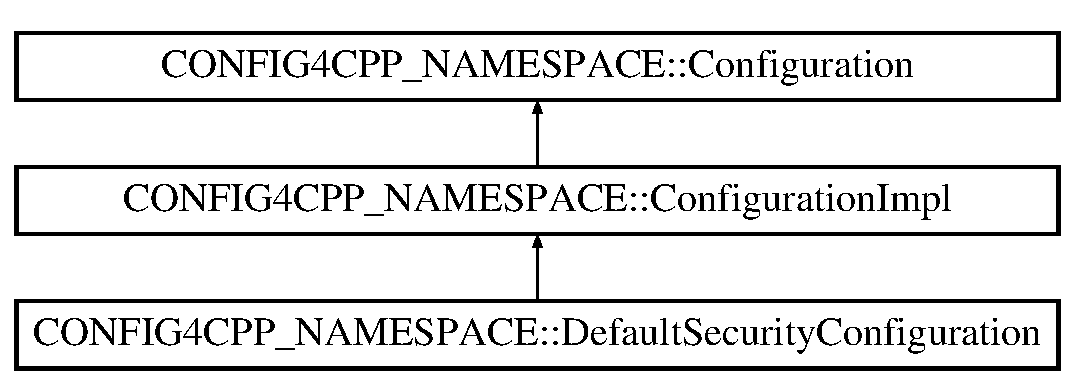
\includegraphics[height=3.000000cm]{classCONFIG4CPP__NAMESPACE_1_1Configuration}
\end{center}
\end{figure}
\subsection*{Public Types}
\begin{DoxyCompactItemize}
\item 
enum {\bfseries Type} \{ \\*
{\bfseries C\-F\-G\-\_\-\-N\-O\-\_\-\-V\-A\-L\-U\-E} = 0, 
{\bfseries C\-F\-G\-\_\-\-S\-T\-R\-I\-N\-G} = 1, 
{\bfseries C\-F\-G\-\_\-\-L\-I\-S\-T} = 2, 
{\bfseries C\-F\-G\-\_\-\-S\-C\-O\-P\-E} = 4, 
\\*
{\bfseries C\-F\-G\-\_\-\-V\-A\-R\-I\-A\-B\-L\-E\-S} = 3, 
{\bfseries C\-F\-G\-\_\-\-S\-C\-O\-P\-E\-\_\-\-A\-N\-D\-\_\-\-V\-A\-R\-S} = 7
 \}
\item 
enum {\bfseries Source\-Type} \{ {\bfseries I\-N\-P\-U\-T\-\_\-\-F\-I\-L\-E}, 
{\bfseries I\-N\-P\-U\-T\-\_\-\-S\-T\-R\-I\-N\-G}, 
{\bfseries I\-N\-P\-U\-T\-\_\-\-E\-X\-E\-C}
 \}
\end{DoxyCompactItemize}
\subsection*{Public Member Functions}
\begin{DoxyCompactItemize}
\item 
\hypertarget{classCONFIG4CPP__NAMESPACE_1_1Configuration_a6b4d9a5b754f030613092e8238ada051}{virtual void {\bfseries destroy} ()}\label{classCONFIG4CPP__NAMESPACE_1_1Configuration_a6b4d9a5b754f030613092e8238ada051}

\item 
\hypertarget{classCONFIG4CPP__NAMESPACE_1_1Configuration_a4ee48cc141113b59c7cdbd684f6f6280}{virtual void {\bfseries set\-Fallback\-Configuration} (\hyperlink{classCONFIG4CPP__NAMESPACE_1_1Configuration}{Configuration} $\ast$cfg)=0}\label{classCONFIG4CPP__NAMESPACE_1_1Configuration_a4ee48cc141113b59c7cdbd684f6f6280}

\item 
\hypertarget{classCONFIG4CPP__NAMESPACE_1_1Configuration_acdabd2bcec65531f37749d05d88bacf0}{virtual void {\bfseries set\-Fallback\-Configuration} (Configuration\-::\-Source\-Type source\-Type, const char $\ast$source, const char $\ast$source\-Description=\char`\"{}\char`\"{})=0  throw (\-Configuration\-Exception)}\label{classCONFIG4CPP__NAMESPACE_1_1Configuration_acdabd2bcec65531f37749d05d88bacf0}

\item 
\hypertarget{classCONFIG4CPP__NAMESPACE_1_1Configuration_a74eb6b4c18c63a6ed458b5d115942908}{virtual const \hyperlink{classCONFIG4CPP__NAMESPACE_1_1Configuration}{Configuration} $\ast$ {\bfseries get\-Fallback\-Configuration} ()=0}\label{classCONFIG4CPP__NAMESPACE_1_1Configuration_a74eb6b4c18c63a6ed458b5d115942908}

\item 
\hypertarget{classCONFIG4CPP__NAMESPACE_1_1Configuration_a10a398ed7d0eb8b331fea8fc64c32679}{virtual void {\bfseries set\-Security\-Configuration} (\hyperlink{classCONFIG4CPP__NAMESPACE_1_1Configuration}{Configuration} $\ast$cfg, bool take\-Ownership, const char $\ast$scope=\char`\"{}\char`\"{})=0  throw (\-Configuration\-Exception)}\label{classCONFIG4CPP__NAMESPACE_1_1Configuration_a10a398ed7d0eb8b331fea8fc64c32679}

\item 
\hypertarget{classCONFIG4CPP__NAMESPACE_1_1Configuration_a7169b8486ab3b27e1d0c76c44dc41025}{virtual void {\bfseries set\-Security\-Configuration} (const char $\ast$cfg\-Input, const char $\ast$scope=\char`\"{}\char`\"{})=0  throw (\-Configuration\-Exception)}\label{classCONFIG4CPP__NAMESPACE_1_1Configuration_a7169b8486ab3b27e1d0c76c44dc41025}

\item 
\hypertarget{classCONFIG4CPP__NAMESPACE_1_1Configuration_a80dbde63ed753da122a831adf4c34f4d}{virtual void {\bfseries get\-Security\-Configuration} (const \hyperlink{classCONFIG4CPP__NAMESPACE_1_1Configuration}{Configuration} $\ast$\&cfg, const char $\ast$\&scope)=0}\label{classCONFIG4CPP__NAMESPACE_1_1Configuration_a80dbde63ed753da122a831adf4c34f4d}

\item 
\hypertarget{classCONFIG4CPP__NAMESPACE_1_1Configuration_a9962e8e2d624ff8b4ddf688098d876ca}{virtual void {\bfseries parse} (Configuration\-::\-Source\-Type source\-Type, const char $\ast$source, const char $\ast$source\-Description=\char`\"{}\char`\"{})=0  throw (\-Configuration\-Exception)}\label{classCONFIG4CPP__NAMESPACE_1_1Configuration_a9962e8e2d624ff8b4ddf688098d876ca}

\item 
\hypertarget{classCONFIG4CPP__NAMESPACE_1_1Configuration_a879e4483675830ae4210eaa906ad9d6c}{void {\bfseries parse} (const char $\ast$source\-Type\-And\-Source)  throw (\-Configuration\-Exception)}\label{classCONFIG4CPP__NAMESPACE_1_1Configuration_a879e4483675830ae4210eaa906ad9d6c}

\item 
\hypertarget{classCONFIG4CPP__NAMESPACE_1_1Configuration_a1606e08d467c38e549800710a385ab30}{virtual const char $\ast$ {\bfseries file\-Name} () const =0}\label{classCONFIG4CPP__NAMESPACE_1_1Configuration_a1606e08d467c38e549800710a385ab30}

\item 
\hypertarget{classCONFIG4CPP__NAMESPACE_1_1Configuration_adfb6ac40fe1cfd06383bc54a7c82e69b}{virtual void {\bfseries list\-Fully\-Scoped\-Names} (const char $\ast$scope, const char $\ast$local\-Name, Type type\-Mask, bool recursive, \hyperlink{classCONFIG4CPP__NAMESPACE_1_1StringVector}{String\-Vector} \&names) const =0  throw (\-Configuration\-Exception)}\label{classCONFIG4CPP__NAMESPACE_1_1Configuration_adfb6ac40fe1cfd06383bc54a7c82e69b}

\item 
\hypertarget{classCONFIG4CPP__NAMESPACE_1_1Configuration_a925700c23182f453b1913184b87db859}{virtual void {\bfseries list\-Fully\-Scoped\-Names} (const char $\ast$scope, const char $\ast$local\-Name, Type type\-Mask, bool recursive, const char $\ast$filter\-Pattern, \hyperlink{classCONFIG4CPP__NAMESPACE_1_1StringVector}{String\-Vector} \&names) const =0  throw (\-Configuration\-Exception)}\label{classCONFIG4CPP__NAMESPACE_1_1Configuration_a925700c23182f453b1913184b87db859}

\item 
\hypertarget{classCONFIG4CPP__NAMESPACE_1_1Configuration_ae00584fdb96a5d9157e3dadc3abd58c4}{virtual void {\bfseries list\-Fully\-Scoped\-Names} (const char $\ast$scope, const char $\ast$local\-Name, Type type\-Mask, bool recursive, const \hyperlink{classCONFIG4CPP__NAMESPACE_1_1StringVector}{String\-Vector} \&filter\-Patterns, \hyperlink{classCONFIG4CPP__NAMESPACE_1_1StringVector}{String\-Vector} \&names) const =0  throw (\-Configuration\-Exception)}\label{classCONFIG4CPP__NAMESPACE_1_1Configuration_ae00584fdb96a5d9157e3dadc3abd58c4}

\item 
\hypertarget{classCONFIG4CPP__NAMESPACE_1_1Configuration_ab8db65ad603a5fe0fb024c7fdd20b934}{virtual void {\bfseries list\-Locally\-Scoped\-Names} (const char $\ast$scope, const char $\ast$local\-Name, Type type\-Mask, bool recursive, \hyperlink{classCONFIG4CPP__NAMESPACE_1_1StringVector}{String\-Vector} \&names) const =0  throw (\-Configuration\-Exception)}\label{classCONFIG4CPP__NAMESPACE_1_1Configuration_ab8db65ad603a5fe0fb024c7fdd20b934}

\item 
\hypertarget{classCONFIG4CPP__NAMESPACE_1_1Configuration_a1b2525a187ee91637a47088acc92e090}{virtual void {\bfseries list\-Locally\-Scoped\-Names} (const char $\ast$scope, const char $\ast$local\-Name, Type type\-Mask, bool recursive, const char $\ast$filter\-Pattern, \hyperlink{classCONFIG4CPP__NAMESPACE_1_1StringVector}{String\-Vector} \&names) const =0  throw (\-Configuration\-Exception)}\label{classCONFIG4CPP__NAMESPACE_1_1Configuration_a1b2525a187ee91637a47088acc92e090}

\item 
\hypertarget{classCONFIG4CPP__NAMESPACE_1_1Configuration_a5e72ebf192e21763966cda00def37d3f}{virtual void {\bfseries list\-Locally\-Scoped\-Names} (const char $\ast$scope, const char $\ast$local\-Name, Type type\-Mask, bool recursive, const \hyperlink{classCONFIG4CPP__NAMESPACE_1_1StringVector}{String\-Vector} \&filter\-Patterns, \hyperlink{classCONFIG4CPP__NAMESPACE_1_1StringVector}{String\-Vector} \&names) const =0  throw (\-Configuration\-Exception)}\label{classCONFIG4CPP__NAMESPACE_1_1Configuration_a5e72ebf192e21763966cda00def37d3f}

\item 
\hypertarget{classCONFIG4CPP__NAMESPACE_1_1Configuration_a54699fc992061b0521fad2df4d6dfaff}{virtual Type {\bfseries type} (const char $\ast$scope, const char $\ast$local\-Name) const =0}\label{classCONFIG4CPP__NAMESPACE_1_1Configuration_a54699fc992061b0521fad2df4d6dfaff}

\item 
\hypertarget{classCONFIG4CPP__NAMESPACE_1_1Configuration_a968327608bf4387631d11680351c25b4}{virtual bool {\bfseries uid\-Equals} (const char $\ast$s1, const char $\ast$s2) const =0}\label{classCONFIG4CPP__NAMESPACE_1_1Configuration_a968327608bf4387631d11680351c25b4}

\item 
\hypertarget{classCONFIG4CPP__NAMESPACE_1_1Configuration_adb4c381219440ecb32f5be2befc463f4}{virtual void {\bfseries expand\-Uid} (\hyperlink{classCONFIG4CPP__NAMESPACE_1_1StringBuffer}{String\-Buffer} \&spelling)=0  throw (\-Configuration\-Exception)}\label{classCONFIG4CPP__NAMESPACE_1_1Configuration_adb4c381219440ecb32f5be2befc463f4}

\item 
\hypertarget{classCONFIG4CPP__NAMESPACE_1_1Configuration_a261d0010d8b27a46991a9feccc916c9c}{virtual const char $\ast$ {\bfseries unexpand\-Uid} (const char $\ast$spelling, \hyperlink{classCONFIG4CPP__NAMESPACE_1_1StringBuffer}{String\-Buffer} \&buf) const =0}\label{classCONFIG4CPP__NAMESPACE_1_1Configuration_a261d0010d8b27a46991a9feccc916c9c}

\item 
\hypertarget{classCONFIG4CPP__NAMESPACE_1_1Configuration_aa7dfe8b35c1cd9d7d18ff62de1894582}{virtual void {\bfseries dump} (\hyperlink{classCONFIG4CPP__NAMESPACE_1_1StringBuffer}{String\-Buffer} \&buf, bool want\-Expanded\-Uid\-Names) const =0}\label{classCONFIG4CPP__NAMESPACE_1_1Configuration_aa7dfe8b35c1cd9d7d18ff62de1894582}

\item 
\hypertarget{classCONFIG4CPP__NAMESPACE_1_1Configuration_a0c705b81a30495e9790ba24e17307819}{virtual void {\bfseries dump} (\hyperlink{classCONFIG4CPP__NAMESPACE_1_1StringBuffer}{String\-Buffer} \&buf, bool want\-Expanded\-Uid\-Names, const char $\ast$scope, const char $\ast$local\-Name) const =0  throw (\-Configuration\-Exception)}\label{classCONFIG4CPP__NAMESPACE_1_1Configuration_a0c705b81a30495e9790ba24e17307819}

\item 
\hypertarget{classCONFIG4CPP__NAMESPACE_1_1Configuration_a5ec6d5ccda2d6aab3c131d1393ece28b}{virtual bool {\bfseries is\-Boolean} (const char $\ast$str) const =0}\label{classCONFIG4CPP__NAMESPACE_1_1Configuration_a5ec6d5ccda2d6aab3c131d1393ece28b}

\item 
\hypertarget{classCONFIG4CPP__NAMESPACE_1_1Configuration_afed6a132f859dbdde3e813817f0dfd99}{virtual bool {\bfseries is\-Int} (const char $\ast$str) const =0}\label{classCONFIG4CPP__NAMESPACE_1_1Configuration_afed6a132f859dbdde3e813817f0dfd99}

\item 
\hypertarget{classCONFIG4CPP__NAMESPACE_1_1Configuration_a33e20bf019112adf8a96e1777ce535fc}{virtual bool {\bfseries is\-Float} (const char $\ast$str) const =0}\label{classCONFIG4CPP__NAMESPACE_1_1Configuration_a33e20bf019112adf8a96e1777ce535fc}

\item 
\hypertarget{classCONFIG4CPP__NAMESPACE_1_1Configuration_af54efe6873b6047cfea57c1e478853c0}{virtual bool {\bfseries is\-Duration\-Microseconds} (const char $\ast$str) const =0}\label{classCONFIG4CPP__NAMESPACE_1_1Configuration_af54efe6873b6047cfea57c1e478853c0}

\item 
\hypertarget{classCONFIG4CPP__NAMESPACE_1_1Configuration_ab31031ad55a6b9cc2e7081d3d81b6785}{virtual bool {\bfseries is\-Duration\-Milliseconds} (const char $\ast$str) const =0}\label{classCONFIG4CPP__NAMESPACE_1_1Configuration_ab31031ad55a6b9cc2e7081d3d81b6785}

\item 
\hypertarget{classCONFIG4CPP__NAMESPACE_1_1Configuration_a6655a4960b5998c9ca22eff7960f6ecb}{virtual bool {\bfseries is\-Duration\-Seconds} (const char $\ast$str) const =0}\label{classCONFIG4CPP__NAMESPACE_1_1Configuration_a6655a4960b5998c9ca22eff7960f6ecb}

\item 
\hypertarget{classCONFIG4CPP__NAMESPACE_1_1Configuration_aef8085f40dd1764bd202b27638632547}{virtual bool {\bfseries is\-Memory\-Size\-Bytes} (const char $\ast$str) const =0}\label{classCONFIG4CPP__NAMESPACE_1_1Configuration_aef8085f40dd1764bd202b27638632547}

\item 
\hypertarget{classCONFIG4CPP__NAMESPACE_1_1Configuration_a153533d8400d62fa5923c86c61a778f4}{virtual bool {\bfseries is\-Memory\-Size\-K\-B} (const char $\ast$str) const =0}\label{classCONFIG4CPP__NAMESPACE_1_1Configuration_a153533d8400d62fa5923c86c61a778f4}

\item 
\hypertarget{classCONFIG4CPP__NAMESPACE_1_1Configuration_ac9dd169927020ccda8a8b8bea723a852}{virtual bool {\bfseries is\-Memory\-Size\-M\-B} (const char $\ast$str) const =0}\label{classCONFIG4CPP__NAMESPACE_1_1Configuration_ac9dd169927020ccda8a8b8bea723a852}

\item 
\hypertarget{classCONFIG4CPP__NAMESPACE_1_1Configuration_ad9cf0942d78dfda6871221911b43e645}{virtual bool {\bfseries is\-Enum} (const char $\ast$str, const \hyperlink{structCONFIG4CPP__NAMESPACE_1_1EnumNameAndValue}{Enum\-Name\-And\-Value} $\ast$enum\-Info, int num\-Enums) const =0}\label{classCONFIG4CPP__NAMESPACE_1_1Configuration_ad9cf0942d78dfda6871221911b43e645}

\item 
\hypertarget{classCONFIG4CPP__NAMESPACE_1_1Configuration_ad50807b263087f742816a6092bb72e14}{virtual bool {\bfseries is\-Float\-With\-Units} (const char $\ast$str, const char $\ast$$\ast$allowed\-Units, int allowed\-Units\-Size) const =0}\label{classCONFIG4CPP__NAMESPACE_1_1Configuration_ad50807b263087f742816a6092bb72e14}

\item 
\hypertarget{classCONFIG4CPP__NAMESPACE_1_1Configuration_a08a300bc4cee2f0f42d05911641124d6}{virtual bool {\bfseries is\-Int\-With\-Units} (const char $\ast$str, const char $\ast$$\ast$allowed\-Units, int allowed\-Units\-Size) const =0}\label{classCONFIG4CPP__NAMESPACE_1_1Configuration_a08a300bc4cee2f0f42d05911641124d6}

\item 
\hypertarget{classCONFIG4CPP__NAMESPACE_1_1Configuration_af132131731f7e2c4910d124b4de1152e}{virtual bool {\bfseries is\-Units\-With\-Float} (const char $\ast$str, const char $\ast$$\ast$allowed\-Units, int allowed\-Units\-Size) const =0}\label{classCONFIG4CPP__NAMESPACE_1_1Configuration_af132131731f7e2c4910d124b4de1152e}

\item 
\hypertarget{classCONFIG4CPP__NAMESPACE_1_1Configuration_a845b2bdfc6a74f1524750d0e002fa155}{virtual bool {\bfseries is\-Units\-With\-Int} (const char $\ast$str, const char $\ast$$\ast$allowed\-Units, int allowed\-Units\-Size) const =0}\label{classCONFIG4CPP__NAMESPACE_1_1Configuration_a845b2bdfc6a74f1524750d0e002fa155}

\item 
\hypertarget{classCONFIG4CPP__NAMESPACE_1_1Configuration_a80f6dcd2137e1fe9672a18d8ed6c22dd}{virtual bool {\bfseries string\-To\-Boolean} (const char $\ast$scope, const char $\ast$local\-Name, const char $\ast$str) const =0  throw (\-Configuration\-Exception)}\label{classCONFIG4CPP__NAMESPACE_1_1Configuration_a80f6dcd2137e1fe9672a18d8ed6c22dd}

\item 
\hypertarget{classCONFIG4CPP__NAMESPACE_1_1Configuration_a1993b784e8ac66c63dcb9ac802661dfd}{virtual int {\bfseries string\-To\-Int} (const char $\ast$scope, const char $\ast$local\-Name, const char $\ast$str) const =0  throw (\-Configuration\-Exception)}\label{classCONFIG4CPP__NAMESPACE_1_1Configuration_a1993b784e8ac66c63dcb9ac802661dfd}

\item 
\hypertarget{classCONFIG4CPP__NAMESPACE_1_1Configuration_af8ce9732bcd6a7079179b98aaaf764fc}{virtual float {\bfseries string\-To\-Float} (const char $\ast$scope, const char $\ast$local\-Name, const char $\ast$str) const =0  throw (\-Configuration\-Exception)}\label{classCONFIG4CPP__NAMESPACE_1_1Configuration_af8ce9732bcd6a7079179b98aaaf764fc}

\item 
\hypertarget{classCONFIG4CPP__NAMESPACE_1_1Configuration_a80a4e0f72cd68ddbf49b641385f0f583}{virtual int {\bfseries string\-To\-Duration\-Seconds} (const char $\ast$scope, const char $\ast$local\-Name, const char $\ast$str) const =0  throw (\-Configuration\-Exception)}\label{classCONFIG4CPP__NAMESPACE_1_1Configuration_a80a4e0f72cd68ddbf49b641385f0f583}

\item 
\hypertarget{classCONFIG4CPP__NAMESPACE_1_1Configuration_ad0f5ff24d51e84e0dea736b8cf08876f}{virtual int {\bfseries string\-To\-Duration\-Milliseconds} (const char $\ast$scope, const char $\ast$local\-Name, const char $\ast$str) const =0  throw (\-Configuration\-Exception)}\label{classCONFIG4CPP__NAMESPACE_1_1Configuration_ad0f5ff24d51e84e0dea736b8cf08876f}

\item 
\hypertarget{classCONFIG4CPP__NAMESPACE_1_1Configuration_a540eed3e343c481b1333e29d2c1f418e}{virtual int {\bfseries string\-To\-Duration\-Microseconds} (const char $\ast$scope, const char $\ast$local\-Name, const char $\ast$str) const =0  throw (\-Configuration\-Exception)}\label{classCONFIG4CPP__NAMESPACE_1_1Configuration_a540eed3e343c481b1333e29d2c1f418e}

\item 
\hypertarget{classCONFIG4CPP__NAMESPACE_1_1Configuration_a35490a4272c0724867821660792cc19f}{virtual int {\bfseries string\-To\-Memory\-Size\-Bytes} (const char $\ast$scope, const char $\ast$local\-Name, const char $\ast$str) const =0  throw (\-Configuration\-Exception)}\label{classCONFIG4CPP__NAMESPACE_1_1Configuration_a35490a4272c0724867821660792cc19f}

\item 
\hypertarget{classCONFIG4CPP__NAMESPACE_1_1Configuration_a4240e07235083dcac0628e7aa02c491c}{virtual int {\bfseries string\-To\-Memory\-Size\-K\-B} (const char $\ast$scope, const char $\ast$local\-Name, const char $\ast$str) const =0  throw (\-Configuration\-Exception)}\label{classCONFIG4CPP__NAMESPACE_1_1Configuration_a4240e07235083dcac0628e7aa02c491c}

\item 
\hypertarget{classCONFIG4CPP__NAMESPACE_1_1Configuration_a2c4feaf8af621754b16caedbd656861b}{virtual int {\bfseries string\-To\-Memory\-Size\-M\-B} (const char $\ast$scope, const char $\ast$local\-Name, const char $\ast$str) const =0  throw (\-Configuration\-Exception)}\label{classCONFIG4CPP__NAMESPACE_1_1Configuration_a2c4feaf8af621754b16caedbd656861b}

\item 
\hypertarget{classCONFIG4CPP__NAMESPACE_1_1Configuration_a64718b9caddf3b07506aa11447708efe}{virtual int {\bfseries string\-To\-Enum} (const char $\ast$scope, const char $\ast$local\-Name, const char $\ast$type\-Name, const char $\ast$str, const \hyperlink{structCONFIG4CPP__NAMESPACE_1_1EnumNameAndValue}{Enum\-Name\-And\-Value} $\ast$enum\-Info, int num\-Enums) const =0  throw (\-Configuration\-Exception)}\label{classCONFIG4CPP__NAMESPACE_1_1Configuration_a64718b9caddf3b07506aa11447708efe}

\item 
\hypertarget{classCONFIG4CPP__NAMESPACE_1_1Configuration_aad3a6f150579d84401941d5cbf3cf0e7}{virtual void {\bfseries string\-To\-Float\-With\-Units} (const char $\ast$scope, const char $\ast$local\-Name, const char $\ast$type\-Name, const char $\ast$str, const char $\ast$$\ast$allowed\-Units, int allowed\-Units\-Size, float \&float\-Result, const char $\ast$\&units\-Result) const =0  throw (\-Configuration\-Exception)}\label{classCONFIG4CPP__NAMESPACE_1_1Configuration_aad3a6f150579d84401941d5cbf3cf0e7}

\item 
\hypertarget{classCONFIG4CPP__NAMESPACE_1_1Configuration_acca91fff8c2cd14d72bd37953697ada5}{virtual void {\bfseries string\-To\-Units\-With\-Float} (const char $\ast$scope, const char $\ast$local\-Name, const char $\ast$type\-Name, const char $\ast$str, const char $\ast$$\ast$allowed\-Units, int allowed\-Units\-Size, float \&float\-Result, const char $\ast$\&units\-Result) const =0  throw (\-Configuration\-Exception)}\label{classCONFIG4CPP__NAMESPACE_1_1Configuration_acca91fff8c2cd14d72bd37953697ada5}

\item 
\hypertarget{classCONFIG4CPP__NAMESPACE_1_1Configuration_a8f360ff006adbd573557344427d42f9f}{virtual void {\bfseries string\-To\-Int\-With\-Units} (const char $\ast$scope, const char $\ast$local\-Name, const char $\ast$type\-Name, const char $\ast$str, const char $\ast$$\ast$allowed\-Units, int allowed\-Units\-Size, int \&int\-Result, const char $\ast$\&units\-Result) const =0  throw (\-Configuration\-Exception)}\label{classCONFIG4CPP__NAMESPACE_1_1Configuration_a8f360ff006adbd573557344427d42f9f}

\item 
\hypertarget{classCONFIG4CPP__NAMESPACE_1_1Configuration_a9a11a56622c5be047b4e6a77164f854b}{virtual void {\bfseries string\-To\-Units\-With\-Int} (const char $\ast$scope, const char $\ast$local\-Name, const char $\ast$type\-Name, const char $\ast$str, const char $\ast$$\ast$allowed\-Units, int allowed\-Units\-Size, int \&int\-Result, const char $\ast$\&units\-Result) const =0  throw (\-Configuration\-Exception)}\label{classCONFIG4CPP__NAMESPACE_1_1Configuration_a9a11a56622c5be047b4e6a77164f854b}

\item 
\hypertarget{classCONFIG4CPP__NAMESPACE_1_1Configuration_a29c789b915ec62161af3f20f0e4f95cc}{virtual const char $\ast$ {\bfseries lookup\-String} (const char $\ast$scope, const char $\ast$local\-Name, const char $\ast$default\-Val) const =0  throw (\-Configuration\-Exception)}\label{classCONFIG4CPP__NAMESPACE_1_1Configuration_a29c789b915ec62161af3f20f0e4f95cc}

\item 
\hypertarget{classCONFIG4CPP__NAMESPACE_1_1Configuration_a8d44332a14b2e39dba5a1876ccafe034}{virtual const char $\ast$ {\bfseries lookup\-String} (const char $\ast$scope, const char $\ast$local\-Name) const =0  throw (\-Configuration\-Exception)}\label{classCONFIG4CPP__NAMESPACE_1_1Configuration_a8d44332a14b2e39dba5a1876ccafe034}

\item 
\hypertarget{classCONFIG4CPP__NAMESPACE_1_1Configuration_adcec7aa081ec51f9db73ccfecf57627f}{virtual void {\bfseries lookup\-List} (const char $\ast$scope, const char $\ast$local\-Name, const char $\ast$$\ast$\&array, int \&array\-Size, const char $\ast$$\ast$default\-Array, int default\-Array\-Size) const =0  throw (\-Configuration\-Exception)}\label{classCONFIG4CPP__NAMESPACE_1_1Configuration_adcec7aa081ec51f9db73ccfecf57627f}

\item 
\hypertarget{classCONFIG4CPP__NAMESPACE_1_1Configuration_a79804bbb433302ff8af28d5f9136c295}{virtual void {\bfseries lookup\-List} (const char $\ast$scope, const char $\ast$local\-Name, const char $\ast$$\ast$\&array, int \&array\-Size) const =0  throw (\-Configuration\-Exception)}\label{classCONFIG4CPP__NAMESPACE_1_1Configuration_a79804bbb433302ff8af28d5f9136c295}

\item 
\hypertarget{classCONFIG4CPP__NAMESPACE_1_1Configuration_ac74b044af14ff94efd5a2c9fba701e9a}{virtual void {\bfseries lookup\-List} (const char $\ast$scope, const char $\ast$local\-Name, \hyperlink{classCONFIG4CPP__NAMESPACE_1_1StringVector}{String\-Vector} \&list, const \hyperlink{classCONFIG4CPP__NAMESPACE_1_1StringVector}{String\-Vector} \&default\-List) const =0  throw (\-Configuration\-Exception)}\label{classCONFIG4CPP__NAMESPACE_1_1Configuration_ac74b044af14ff94efd5a2c9fba701e9a}

\item 
\hypertarget{classCONFIG4CPP__NAMESPACE_1_1Configuration_a521f2aab1656d6e5167a42d160dee252}{virtual void {\bfseries lookup\-List} (const char $\ast$scope, const char $\ast$local\-Name, \hyperlink{classCONFIG4CPP__NAMESPACE_1_1StringVector}{String\-Vector} \&list) const =0  throw (\-Configuration\-Exception)}\label{classCONFIG4CPP__NAMESPACE_1_1Configuration_a521f2aab1656d6e5167a42d160dee252}

\item 
\hypertarget{classCONFIG4CPP__NAMESPACE_1_1Configuration_af8e8ace7fe8ba60b580dc7575fb8218f}{virtual int {\bfseries lookup\-Int} (const char $\ast$scope, const char $\ast$local\-Name, int default\-Val) const =0  throw (\-Configuration\-Exception)}\label{classCONFIG4CPP__NAMESPACE_1_1Configuration_af8e8ace7fe8ba60b580dc7575fb8218f}

\item 
\hypertarget{classCONFIG4CPP__NAMESPACE_1_1Configuration_a5be802f9ec20e88ecc6e0312fdfb1fb5}{virtual int {\bfseries lookup\-Int} (const char $\ast$scope, const char $\ast$local\-Name) const =0  throw (\-Configuration\-Exception)}\label{classCONFIG4CPP__NAMESPACE_1_1Configuration_a5be802f9ec20e88ecc6e0312fdfb1fb5}

\item 
\hypertarget{classCONFIG4CPP__NAMESPACE_1_1Configuration_aa95a3d368ba9cc6e9504c7d7e76b0a86}{virtual float {\bfseries lookup\-Float} (const char $\ast$scope, const char $\ast$local\-Name, float default\-Val) const =0  throw (\-Configuration\-Exception)}\label{classCONFIG4CPP__NAMESPACE_1_1Configuration_aa95a3d368ba9cc6e9504c7d7e76b0a86}

\item 
\hypertarget{classCONFIG4CPP__NAMESPACE_1_1Configuration_a9abd2d9569ce735829e20456d663938c}{virtual float {\bfseries lookup\-Float} (const char $\ast$scope, const char $\ast$local\-Name) const =0  throw (\-Configuration\-Exception)}\label{classCONFIG4CPP__NAMESPACE_1_1Configuration_a9abd2d9569ce735829e20456d663938c}

\item 
\hypertarget{classCONFIG4CPP__NAMESPACE_1_1Configuration_a2ae8691ea64b67ba84d21e9512f44b24}{virtual int {\bfseries lookup\-Enum} (const char $\ast$scope, const char $\ast$local\-Name, const char $\ast$type\-Name, const \hyperlink{structCONFIG4CPP__NAMESPACE_1_1EnumNameAndValue}{Enum\-Name\-And\-Value} $\ast$enum\-Info, int num\-Enums, const char $\ast$default\-Val) const =0  throw (\-Configuration\-Exception)}\label{classCONFIG4CPP__NAMESPACE_1_1Configuration_a2ae8691ea64b67ba84d21e9512f44b24}

\item 
\hypertarget{classCONFIG4CPP__NAMESPACE_1_1Configuration_adfed2a57303fdb4c8e7191832890f750}{virtual int {\bfseries lookup\-Enum} (const char $\ast$scope, const char $\ast$local\-Name, const char $\ast$type\-Name, const \hyperlink{structCONFIG4CPP__NAMESPACE_1_1EnumNameAndValue}{Enum\-Name\-And\-Value} $\ast$enum\-Info, int num\-Enums, int default\-Val) const =0  throw (\-Configuration\-Exception)}\label{classCONFIG4CPP__NAMESPACE_1_1Configuration_adfed2a57303fdb4c8e7191832890f750}

\item 
\hypertarget{classCONFIG4CPP__NAMESPACE_1_1Configuration_a604084c81180661f830c4da1c0fe9366}{virtual int {\bfseries lookup\-Enum} (const char $\ast$scope, const char $\ast$local\-Name, const char $\ast$type\-Name, const \hyperlink{structCONFIG4CPP__NAMESPACE_1_1EnumNameAndValue}{Enum\-Name\-And\-Value} $\ast$enum\-Info, int num\-Enums) const =0  throw (\-Configuration\-Exception)}\label{classCONFIG4CPP__NAMESPACE_1_1Configuration_a604084c81180661f830c4da1c0fe9366}

\item 
\hypertarget{classCONFIG4CPP__NAMESPACE_1_1Configuration_a292fcba7dc020393a230a1190e551184}{virtual bool {\bfseries lookup\-Boolean} (const char $\ast$scope, const char $\ast$local\-Name, bool default\-Val) const =0  throw (\-Configuration\-Exception)}\label{classCONFIG4CPP__NAMESPACE_1_1Configuration_a292fcba7dc020393a230a1190e551184}

\item 
\hypertarget{classCONFIG4CPP__NAMESPACE_1_1Configuration_aeef7e63e598546b9713ee1a2b9517b9e}{virtual bool {\bfseries lookup\-Boolean} (const char $\ast$scope, const char $\ast$local\-Name) const =0  throw (\-Configuration\-Exception)}\label{classCONFIG4CPP__NAMESPACE_1_1Configuration_aeef7e63e598546b9713ee1a2b9517b9e}

\item 
\hypertarget{classCONFIG4CPP__NAMESPACE_1_1Configuration_a06356d620f19cc192b43c5663fe2e73f}{virtual void {\bfseries lookup\-Float\-With\-Units} (const char $\ast$scope, const char $\ast$local\-Name, const char $\ast$type\-Name, const char $\ast$$\ast$allowed\-Units, int allowed\-Units\-Size, float \&float\-Result, const char $\ast$\&units\-Result) const =0  throw (\-Configuration\-Exception)}\label{classCONFIG4CPP__NAMESPACE_1_1Configuration_a06356d620f19cc192b43c5663fe2e73f}

\item 
\hypertarget{classCONFIG4CPP__NAMESPACE_1_1Configuration_a1c9cae8721b367b5181f95091a0d9f77}{virtual void {\bfseries lookup\-Float\-With\-Units} (const char $\ast$scope, const char $\ast$local\-Name, const char $\ast$type\-Name, const char $\ast$$\ast$allowed\-Units, int allowed\-Units\-Size, float \&float\-Result, const char $\ast$\&units\-Result, float default\-Float, const char $\ast$default\-Units) const =0  throw (\-Configuration\-Exception)}\label{classCONFIG4CPP__NAMESPACE_1_1Configuration_a1c9cae8721b367b5181f95091a0d9f77}

\item 
\hypertarget{classCONFIG4CPP__NAMESPACE_1_1Configuration_a604b3d82b8e688f8f97326ef86afa763}{virtual void {\bfseries lookup\-Units\-With\-Float} (const char $\ast$scope, const char $\ast$local\-Name, const char $\ast$type\-Name, const char $\ast$$\ast$allowed\-Units, int allowed\-Units\-Size, float \&float\-Result, const char $\ast$\&units\-Result) const =0  throw (\-Configuration\-Exception)}\label{classCONFIG4CPP__NAMESPACE_1_1Configuration_a604b3d82b8e688f8f97326ef86afa763}

\item 
\hypertarget{classCONFIG4CPP__NAMESPACE_1_1Configuration_a9a30a5b4f012a9b8b2e19361a272b049}{virtual void {\bfseries lookup\-Units\-With\-Float} (const char $\ast$scope, const char $\ast$local\-Name, const char $\ast$type\-Name, const char $\ast$$\ast$allowed\-Units, int allowed\-Units\-Size, float \&float\-Result, const char $\ast$\&units\-Result, float default\-Float, const char $\ast$default\-Units) const =0  throw (\-Configuration\-Exception)}\label{classCONFIG4CPP__NAMESPACE_1_1Configuration_a9a30a5b4f012a9b8b2e19361a272b049}

\item 
\hypertarget{classCONFIG4CPP__NAMESPACE_1_1Configuration_a7182f206efac4765215534807d1c2485}{virtual void {\bfseries lookup\-Int\-With\-Units} (const char $\ast$scope, const char $\ast$local\-Name, const char $\ast$type\-Name, const char $\ast$$\ast$allowed\-Units, int allowed\-Units\-Size, int \&int\-Result, const char $\ast$\&units\-Result) const =0  throw (\-Configuration\-Exception)}\label{classCONFIG4CPP__NAMESPACE_1_1Configuration_a7182f206efac4765215534807d1c2485}

\item 
\hypertarget{classCONFIG4CPP__NAMESPACE_1_1Configuration_a34ecd7e12e787054b7cc49de6570d7f4}{virtual void {\bfseries lookup\-Int\-With\-Units} (const char $\ast$scope, const char $\ast$local\-Name, const char $\ast$type\-Name, const char $\ast$$\ast$allowed\-Units, int allowed\-Units\-Size, int \&int\-Result, const char $\ast$\&units\-Result, int default\-Int, const char $\ast$default\-Units) const =0  throw (\-Configuration\-Exception)}\label{classCONFIG4CPP__NAMESPACE_1_1Configuration_a34ecd7e12e787054b7cc49de6570d7f4}

\item 
\hypertarget{classCONFIG4CPP__NAMESPACE_1_1Configuration_aeef6917fd510cce95021efe7146f5f2d}{virtual void {\bfseries lookup\-Units\-With\-Int} (const char $\ast$scope, const char $\ast$local\-Name, const char $\ast$type\-Name, const char $\ast$$\ast$allowed\-Units, int allowed\-Units\-Size, int \&int\-Result, const char $\ast$\&units\-Result) const =0  throw (\-Configuration\-Exception)}\label{classCONFIG4CPP__NAMESPACE_1_1Configuration_aeef6917fd510cce95021efe7146f5f2d}

\item 
\hypertarget{classCONFIG4CPP__NAMESPACE_1_1Configuration_aaf749dca18f5dd7d82b49f1bc0ae5815}{virtual void {\bfseries lookup\-Units\-With\-Int} (const char $\ast$scope, const char $\ast$local\-Name, const char $\ast$type\-Name, const char $\ast$$\ast$allowed\-Units, int allowed\-Units\-Size, int \&int\-Result, const char $\ast$\&units\-Result, int default\-Int, const char $\ast$default\-Units) const =0  throw (\-Configuration\-Exception)}\label{classCONFIG4CPP__NAMESPACE_1_1Configuration_aaf749dca18f5dd7d82b49f1bc0ae5815}

\item 
\hypertarget{classCONFIG4CPP__NAMESPACE_1_1Configuration_ae765bb1acc8740a92d1ed451c210267a}{virtual int {\bfseries lookup\-Duration\-Microseconds} (const char $\ast$scope, const char $\ast$local\-Name, int default\-Val) const =0  throw (\-Configuration\-Exception)}\label{classCONFIG4CPP__NAMESPACE_1_1Configuration_ae765bb1acc8740a92d1ed451c210267a}

\item 
\hypertarget{classCONFIG4CPP__NAMESPACE_1_1Configuration_a411801a2337daf86b335cc9fa2c6d6fb}{virtual int {\bfseries lookup\-Duration\-Microseconds} (const char $\ast$scope, const char $\ast$local\-Name) const =0  throw (\-Configuration\-Exception)}\label{classCONFIG4CPP__NAMESPACE_1_1Configuration_a411801a2337daf86b335cc9fa2c6d6fb}

\item 
\hypertarget{classCONFIG4CPP__NAMESPACE_1_1Configuration_ac3f5af404012b6b1a3cfb2b177fb8b62}{virtual int {\bfseries lookup\-Duration\-Milliseconds} (const char $\ast$scope, const char $\ast$local\-Name, int default\-Val) const =0  throw (\-Configuration\-Exception)}\label{classCONFIG4CPP__NAMESPACE_1_1Configuration_ac3f5af404012b6b1a3cfb2b177fb8b62}

\item 
\hypertarget{classCONFIG4CPP__NAMESPACE_1_1Configuration_a060f220e870ad75ba029123283b7772f}{virtual int {\bfseries lookup\-Duration\-Milliseconds} (const char $\ast$scope, const char $\ast$local\-Name) const =0  throw (\-Configuration\-Exception)}\label{classCONFIG4CPP__NAMESPACE_1_1Configuration_a060f220e870ad75ba029123283b7772f}

\item 
\hypertarget{classCONFIG4CPP__NAMESPACE_1_1Configuration_a3b4815de4f40b8a75e8399f298041b8a}{virtual int {\bfseries lookup\-Duration\-Seconds} (const char $\ast$scope, const char $\ast$local\-Name, int default\-Val) const =0  throw (\-Configuration\-Exception)}\label{classCONFIG4CPP__NAMESPACE_1_1Configuration_a3b4815de4f40b8a75e8399f298041b8a}

\item 
\hypertarget{classCONFIG4CPP__NAMESPACE_1_1Configuration_af01f653956f637de24a7d3c3b24345e0}{virtual int {\bfseries lookup\-Duration\-Seconds} (const char $\ast$scope, const char $\ast$local\-Name) const =0  throw (\-Configuration\-Exception)}\label{classCONFIG4CPP__NAMESPACE_1_1Configuration_af01f653956f637de24a7d3c3b24345e0}

\item 
\hypertarget{classCONFIG4CPP__NAMESPACE_1_1Configuration_a2cf4fb9d8b7cae7a7faba0e92911ecae}{virtual int {\bfseries lookup\-Memory\-Size\-Bytes} (const char $\ast$scope, const char $\ast$local\-Name, int default\-Val) const =0  throw (\-Configuration\-Exception)}\label{classCONFIG4CPP__NAMESPACE_1_1Configuration_a2cf4fb9d8b7cae7a7faba0e92911ecae}

\item 
\hypertarget{classCONFIG4CPP__NAMESPACE_1_1Configuration_ae37820eea8f3a35858f37876fa1ee921}{virtual int {\bfseries lookup\-Memory\-Size\-Bytes} (const char $\ast$scope, const char $\ast$local\-Name) const =0  throw (\-Configuration\-Exception)}\label{classCONFIG4CPP__NAMESPACE_1_1Configuration_ae37820eea8f3a35858f37876fa1ee921}

\item 
\hypertarget{classCONFIG4CPP__NAMESPACE_1_1Configuration_a60223b88f9f8ec41d1551403ba3ea192}{virtual int {\bfseries lookup\-Memory\-Size\-K\-B} (const char $\ast$scope, const char $\ast$local\-Name, int default\-Val) const =0  throw (\-Configuration\-Exception)}\label{classCONFIG4CPP__NAMESPACE_1_1Configuration_a60223b88f9f8ec41d1551403ba3ea192}

\item 
\hypertarget{classCONFIG4CPP__NAMESPACE_1_1Configuration_a44dd9f98cff623000df1e6eca7a92f4c}{virtual int {\bfseries lookup\-Memory\-Size\-K\-B} (const char $\ast$scope, const char $\ast$local\-Name) const =0  throw (\-Configuration\-Exception)}\label{classCONFIG4CPP__NAMESPACE_1_1Configuration_a44dd9f98cff623000df1e6eca7a92f4c}

\item 
\hypertarget{classCONFIG4CPP__NAMESPACE_1_1Configuration_adbfc936338d4c86e7c2ce9d1efb38ac3}{virtual int {\bfseries lookup\-Memory\-Size\-M\-B} (const char $\ast$scope, const char $\ast$local\-Name, int default\-Val) const =0  throw (\-Configuration\-Exception)}\label{classCONFIG4CPP__NAMESPACE_1_1Configuration_adbfc936338d4c86e7c2ce9d1efb38ac3}

\item 
\hypertarget{classCONFIG4CPP__NAMESPACE_1_1Configuration_af4c75331ada2a8ea767759e598dc4813}{virtual int {\bfseries lookup\-Memory\-Size\-M\-B} (const char $\ast$scope, const char $\ast$local\-Name) const =0  throw (\-Configuration\-Exception)}\label{classCONFIG4CPP__NAMESPACE_1_1Configuration_af4c75331ada2a8ea767759e598dc4813}

\item 
\hypertarget{classCONFIG4CPP__NAMESPACE_1_1Configuration_a6acec433039e028637a396dacbabf06b}{virtual void {\bfseries lookup\-Scope} (const char $\ast$scope, const char $\ast$local\-Name) const =0  throw (\-Configuration\-Exception)}\label{classCONFIG4CPP__NAMESPACE_1_1Configuration_a6acec433039e028637a396dacbabf06b}

\item 
\hypertarget{classCONFIG4CPP__NAMESPACE_1_1Configuration_ab7050a889854c6925338ff9b6b751e82}{virtual void {\bfseries insert\-String} (const char $\ast$scope, const char $\ast$local\-Name, const char $\ast$str\-Value)=0  throw (\-Configuration\-Exception)}\label{classCONFIG4CPP__NAMESPACE_1_1Configuration_ab7050a889854c6925338ff9b6b751e82}

\item 
\hypertarget{classCONFIG4CPP__NAMESPACE_1_1Configuration_a3e1c09a93f7ac0abe44368d9a65afd23}{virtual void {\bfseries insert\-List} (const char $\ast$scope, const char $\ast$local\-Name, const char $\ast$$\ast$array, int array\-Size)=0  throw (\-Configuration\-Exception)}\label{classCONFIG4CPP__NAMESPACE_1_1Configuration_a3e1c09a93f7ac0abe44368d9a65afd23}

\item 
\hypertarget{classCONFIG4CPP__NAMESPACE_1_1Configuration_a0bc15285cf5f7ea5aa2ccf26a94590a3}{virtual void {\bfseries insert\-List} (const char $\ast$scope, const char $\ast$local\-Name, const char $\ast$$\ast$null\-Terminated\-Array)=0  throw (\-Configuration\-Exception)}\label{classCONFIG4CPP__NAMESPACE_1_1Configuration_a0bc15285cf5f7ea5aa2ccf26a94590a3}

\item 
\hypertarget{classCONFIG4CPP__NAMESPACE_1_1Configuration_a6496260411337a65f0d82fae0ff552c6}{virtual void {\bfseries insert\-List} (const char $\ast$scope, const char $\ast$local\-Name, const \hyperlink{classCONFIG4CPP__NAMESPACE_1_1StringVector}{String\-Vector} \&vec)=0  throw (\-Configuration\-Exception)}\label{classCONFIG4CPP__NAMESPACE_1_1Configuration_a6496260411337a65f0d82fae0ff552c6}

\item 
\hypertarget{classCONFIG4CPP__NAMESPACE_1_1Configuration_a497d3a52000cdf672ad893db8ea1ccef}{virtual void {\bfseries ensure\-Scope\-Exists} (const char $\ast$scope, const char $\ast$local\-Name)=0  throw (\-Configuration\-Exception)}\label{classCONFIG4CPP__NAMESPACE_1_1Configuration_a497d3a52000cdf672ad893db8ea1ccef}

\item 
\hypertarget{classCONFIG4CPP__NAMESPACE_1_1Configuration_abe28bb7ebf77e8b98847cbc457f58bc7}{virtual void {\bfseries remove} (const char $\ast$scope, const char $\ast$local\-Name)=0  throw (\-Configuration\-Exception)}\label{classCONFIG4CPP__NAMESPACE_1_1Configuration_abe28bb7ebf77e8b98847cbc457f58bc7}

\item 
\hypertarget{classCONFIG4CPP__NAMESPACE_1_1Configuration_ab4b0970b66d66ef42f63f7701c3ca928}{virtual void {\bfseries empty} ()=0}\label{classCONFIG4CPP__NAMESPACE_1_1Configuration_ab4b0970b66d66ef42f63f7701c3ca928}

\end{DoxyCompactItemize}
\subsection*{Static Public Member Functions}
\begin{DoxyCompactItemize}
\item 
\hypertarget{classCONFIG4CPP__NAMESPACE_1_1Configuration_afc76ea7c7408eaa284f7f78280d7ea0a}{static \hyperlink{classCONFIG4CPP__NAMESPACE_1_1Configuration}{Configuration} $\ast$ {\bfseries create} ()}\label{classCONFIG4CPP__NAMESPACE_1_1Configuration_afc76ea7c7408eaa284f7f78280d7ea0a}

\item 
\hypertarget{classCONFIG4CPP__NAMESPACE_1_1Configuration_a80e05a00907f4120cd854a0e9eb3a984}{static void {\bfseries merge\-Names} (const char $\ast$scope, const char $\ast$local\-Name, \hyperlink{classCONFIG4CPP__NAMESPACE_1_1StringBuffer}{String\-Buffer} \&fully\-Scoped\-Name)}\label{classCONFIG4CPP__NAMESPACE_1_1Configuration_a80e05a00907f4120cd854a0e9eb3a984}

\item 
\hypertarget{classCONFIG4CPP__NAMESPACE_1_1Configuration_a1f2a054198d9049975b20fc321f276b7}{static int {\bfseries mbstrlen} (const char $\ast$str)}\label{classCONFIG4CPP__NAMESPACE_1_1Configuration_a1f2a054198d9049975b20fc321f276b7}

\item 
\hypertarget{classCONFIG4CPP__NAMESPACE_1_1Configuration_a53dbcaf469fb63b08343575c983d16f6}{static bool {\bfseries pattern\-Match} (const char $\ast$str, const char $\ast$pattern)}\label{classCONFIG4CPP__NAMESPACE_1_1Configuration_a53dbcaf469fb63b08343575c983d16f6}

\end{DoxyCompactItemize}


The documentation for this class was generated from the following files\-:\begin{DoxyCompactItemize}
\item 
src/configuration/config4cpp/include/config4cpp/Configuration.\-h\item 
src/configuration/config4cpp/src/Configuration.\-cpp\end{DoxyCompactItemize}

\hypertarget{classCONFIG4CPP__NAMESPACE_1_1ConfigurationException}{\section{C\-O\-N\-F\-I\-G4\-C\-P\-P\-\_\-\-N\-A\-M\-E\-S\-P\-A\-C\-E\-:\-:Configuration\-Exception Class Reference}
\label{classCONFIG4CPP__NAMESPACE_1_1ConfigurationException}\index{C\-O\-N\-F\-I\-G4\-C\-P\-P\-\_\-\-N\-A\-M\-E\-S\-P\-A\-C\-E\-::\-Configuration\-Exception@{C\-O\-N\-F\-I\-G4\-C\-P\-P\-\_\-\-N\-A\-M\-E\-S\-P\-A\-C\-E\-::\-Configuration\-Exception}}
}
\subsection*{Public Member Functions}
\begin{DoxyCompactItemize}
\item 
\hypertarget{classCONFIG4CPP__NAMESPACE_1_1ConfigurationException_afcf62392434113e9f5b7277916b1bdfb}{{\bfseries Configuration\-Exception} (const char $\ast$str)}\label{classCONFIG4CPP__NAMESPACE_1_1ConfigurationException_afcf62392434113e9f5b7277916b1bdfb}

\item 
\hypertarget{classCONFIG4CPP__NAMESPACE_1_1ConfigurationException_ae2dee9c0232786ca5cd15a2e3db108b0}{{\bfseries Configuration\-Exception} (const \hyperlink{classCONFIG4CPP__NAMESPACE_1_1ConfigurationException}{Configuration\-Exception} \&o)}\label{classCONFIG4CPP__NAMESPACE_1_1ConfigurationException_ae2dee9c0232786ca5cd15a2e3db108b0}

\item 
\hypertarget{classCONFIG4CPP__NAMESPACE_1_1ConfigurationException_a42c394a476808848924d096ec6fbb186}{const char $\ast$ {\bfseries c\-\_\-str} () const }\label{classCONFIG4CPP__NAMESPACE_1_1ConfigurationException_a42c394a476808848924d096ec6fbb186}

\end{DoxyCompactItemize}


The documentation for this class was generated from the following files\-:\begin{DoxyCompactItemize}
\item 
src/configuration/config4cpp/include/config4cpp/Configuration\-Exception.\-h\item 
src/configuration/config4cpp/src/Configuration\-Exception.\-cpp\end{DoxyCompactItemize}

\hypertarget{classCONFIG4CPP__NAMESPACE_1_1ConfigurationImpl}{\section{C\-O\-N\-F\-I\-G4\-C\-P\-P\-\_\-\-N\-A\-M\-E\-S\-P\-A\-C\-E\-:\-:Configuration\-Impl Class Reference}
\label{classCONFIG4CPP__NAMESPACE_1_1ConfigurationImpl}\index{C\-O\-N\-F\-I\-G4\-C\-P\-P\-\_\-\-N\-A\-M\-E\-S\-P\-A\-C\-E\-::\-Configuration\-Impl@{C\-O\-N\-F\-I\-G4\-C\-P\-P\-\_\-\-N\-A\-M\-E\-S\-P\-A\-C\-E\-::\-Configuration\-Impl}}
}
Inheritance diagram for C\-O\-N\-F\-I\-G4\-C\-P\-P\-\_\-\-N\-A\-M\-E\-S\-P\-A\-C\-E\-:\-:Configuration\-Impl\-:\begin{figure}[H]
\begin{center}
\leavevmode
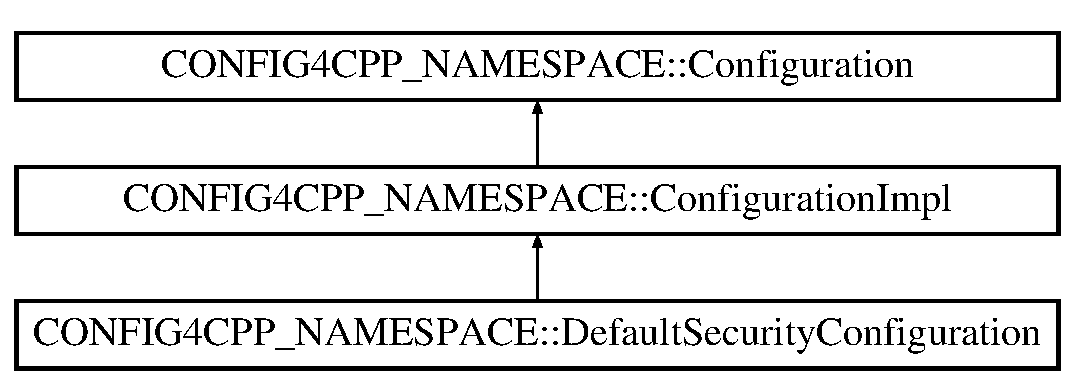
\includegraphics[height=3.000000cm]{classCONFIG4CPP__NAMESPACE_1_1ConfigurationImpl}
\end{center}
\end{figure}
\subsection*{Public Member Functions}
\begin{DoxyCompactItemize}
\item 
\hypertarget{classCONFIG4CPP__NAMESPACE_1_1ConfigurationImpl_ad14bdefa48472b366e67fb1b549c5d9f}{virtual void {\bfseries set\-Fallback\-Configuration} (\hyperlink{classCONFIG4CPP__NAMESPACE_1_1Configuration}{Configuration} $\ast$cfg)}\label{classCONFIG4CPP__NAMESPACE_1_1ConfigurationImpl_ad14bdefa48472b366e67fb1b549c5d9f}

\item 
\hypertarget{classCONFIG4CPP__NAMESPACE_1_1ConfigurationImpl_ad5b85c0eb0f7e8af317f0bfaa015101a}{virtual void {\bfseries set\-Fallback\-Configuration} (Configuration\-::\-Source\-Type source\-Type, const char $\ast$source, const char $\ast$source\-Description=\char`\"{}\char`\"{})  throw (\-Configuration\-Exception)}\label{classCONFIG4CPP__NAMESPACE_1_1ConfigurationImpl_ad5b85c0eb0f7e8af317f0bfaa015101a}

\item 
\hypertarget{classCONFIG4CPP__NAMESPACE_1_1ConfigurationImpl_af93de4baebfdf1d1a6425292bb6269fc}{virtual const \hyperlink{classCONFIG4CPP__NAMESPACE_1_1Configuration}{Configuration} $\ast$ {\bfseries get\-Fallback\-Configuration} ()}\label{classCONFIG4CPP__NAMESPACE_1_1ConfigurationImpl_af93de4baebfdf1d1a6425292bb6269fc}

\item 
\hypertarget{classCONFIG4CPP__NAMESPACE_1_1ConfigurationImpl_a20fb84b7845206d9b44f3703b82668e2}{virtual void {\bfseries set\-Security\-Configuration} (\hyperlink{classCONFIG4CPP__NAMESPACE_1_1Configuration}{Configuration} $\ast$cfg, bool take\-Ownership, const char $\ast$scope=\char`\"{}\char`\"{})  throw (\-Configuration\-Exception)}\label{classCONFIG4CPP__NAMESPACE_1_1ConfigurationImpl_a20fb84b7845206d9b44f3703b82668e2}

\item 
\hypertarget{classCONFIG4CPP__NAMESPACE_1_1ConfigurationImpl_af28f20be9686e4ccacab522182a0ec2b}{virtual void {\bfseries set\-Security\-Configuration} (const char $\ast$cfg\-Input, const char $\ast$scope=\char`\"{}\char`\"{})  throw (\-Configuration\-Exception)}\label{classCONFIG4CPP__NAMESPACE_1_1ConfigurationImpl_af28f20be9686e4ccacab522182a0ec2b}

\item 
\hypertarget{classCONFIG4CPP__NAMESPACE_1_1ConfigurationImpl_abe6da19af65d96835ffe952b385fbb3a}{virtual void {\bfseries get\-Security\-Configuration} (const \hyperlink{classCONFIG4CPP__NAMESPACE_1_1Configuration}{Configuration} $\ast$\&cfg, const char $\ast$\&scope)}\label{classCONFIG4CPP__NAMESPACE_1_1ConfigurationImpl_abe6da19af65d96835ffe952b385fbb3a}

\item 
\hypertarget{classCONFIG4CPP__NAMESPACE_1_1ConfigurationImpl_ad93978e0b1013b181380c9e22947d54f}{virtual void {\bfseries parse} (Configuration\-::\-Source\-Type source\-Type, const char $\ast$source, const char $\ast$source\-Description=\char`\"{}\char`\"{})  throw (\-Configuration\-Exception)}\label{classCONFIG4CPP__NAMESPACE_1_1ConfigurationImpl_ad93978e0b1013b181380c9e22947d54f}

\item 
\hypertarget{classCONFIG4CPP__NAMESPACE_1_1ConfigurationImpl_ac39e0c0a64c5f79a0b29af764595e3fc}{virtual const char $\ast$ {\bfseries file\-Name} () const }\label{classCONFIG4CPP__NAMESPACE_1_1ConfigurationImpl_ac39e0c0a64c5f79a0b29af764595e3fc}

\item 
\hypertarget{classCONFIG4CPP__NAMESPACE_1_1ConfigurationImpl_a1280cad50a7164d0ed53822f6110e7c8}{virtual Type {\bfseries type} (const char $\ast$scope, const char $\ast$local\-Name) const }\label{classCONFIG4CPP__NAMESPACE_1_1ConfigurationImpl_a1280cad50a7164d0ed53822f6110e7c8}

\item 
\hypertarget{classCONFIG4CPP__NAMESPACE_1_1ConfigurationImpl_aef9abe659ffe8985e987b2ec78890059}{virtual void {\bfseries list\-Fully\-Scoped\-Names} (const char $\ast$scope, const char $\ast$local\-Name, Type type\-Mask, bool recursive, \hyperlink{classCONFIG4CPP__NAMESPACE_1_1StringVector}{String\-Vector} \&names) const   throw (\-Configuration\-Exception)}\label{classCONFIG4CPP__NAMESPACE_1_1ConfigurationImpl_aef9abe659ffe8985e987b2ec78890059}

\item 
\hypertarget{classCONFIG4CPP__NAMESPACE_1_1ConfigurationImpl_a7414a94c5bc92fc280e75a6af9fe3535}{virtual void {\bfseries list\-Fully\-Scoped\-Names} (const char $\ast$scope, const char $\ast$local\-Name, Type type\-Mask, bool recursive, const char $\ast$filter\-Pattern, \hyperlink{classCONFIG4CPP__NAMESPACE_1_1StringVector}{String\-Vector} \&names) const   throw (\-Configuration\-Exception)}\label{classCONFIG4CPP__NAMESPACE_1_1ConfigurationImpl_a7414a94c5bc92fc280e75a6af9fe3535}

\item 
\hypertarget{classCONFIG4CPP__NAMESPACE_1_1ConfigurationImpl_ac84bf4827fde0aa7a23d0d15052247ae}{virtual void {\bfseries list\-Fully\-Scoped\-Names} (const char $\ast$scope, const char $\ast$local\-Name, Type type\-Mask, bool recursive, const \hyperlink{classCONFIG4CPP__NAMESPACE_1_1StringVector}{String\-Vector} \&filter\-Patterns, \hyperlink{classCONFIG4CPP__NAMESPACE_1_1StringVector}{String\-Vector} \&names) const   throw (\-Configuration\-Exception)}\label{classCONFIG4CPP__NAMESPACE_1_1ConfigurationImpl_ac84bf4827fde0aa7a23d0d15052247ae}

\item 
\hypertarget{classCONFIG4CPP__NAMESPACE_1_1ConfigurationImpl_a4aa1415b61d5e36a36f3d218cc8572dc}{virtual void {\bfseries list\-Locally\-Scoped\-Names} (const char $\ast$scope, const char $\ast$local\-Name, Type type\-Mask, bool recursive, \hyperlink{classCONFIG4CPP__NAMESPACE_1_1StringVector}{String\-Vector} \&names) const   throw (\-Configuration\-Exception)}\label{classCONFIG4CPP__NAMESPACE_1_1ConfigurationImpl_a4aa1415b61d5e36a36f3d218cc8572dc}

\item 
\hypertarget{classCONFIG4CPP__NAMESPACE_1_1ConfigurationImpl_a871970a1c874e53f80a679bbe4e652ed}{virtual void {\bfseries list\-Locally\-Scoped\-Names} (const char $\ast$scope, const char $\ast$local\-Name, Type type\-Mask, bool recursive, const char $\ast$filter\-Pattern, \hyperlink{classCONFIG4CPP__NAMESPACE_1_1StringVector}{String\-Vector} \&names) const   throw (\-Configuration\-Exception)}\label{classCONFIG4CPP__NAMESPACE_1_1ConfigurationImpl_a871970a1c874e53f80a679bbe4e652ed}

\item 
\hypertarget{classCONFIG4CPP__NAMESPACE_1_1ConfigurationImpl_af48b44d00f90bc916590b6a25c1617d7}{virtual void {\bfseries list\-Locally\-Scoped\-Names} (const char $\ast$scope, const char $\ast$local\-Name, Type type\-Mask, bool recursive, const \hyperlink{classCONFIG4CPP__NAMESPACE_1_1StringVector}{String\-Vector} \&filter\-Patterns, \hyperlink{classCONFIG4CPP__NAMESPACE_1_1StringVector}{String\-Vector} \&names) const   throw (\-Configuration\-Exception)}\label{classCONFIG4CPP__NAMESPACE_1_1ConfigurationImpl_af48b44d00f90bc916590b6a25c1617d7}

\item 
\hypertarget{classCONFIG4CPP__NAMESPACE_1_1ConfigurationImpl_ae167d0095c9ddf16c8db8ecb02b529ca}{virtual bool {\bfseries uid\-Equals} (const char $\ast$s1, const char $\ast$s2) const }\label{classCONFIG4CPP__NAMESPACE_1_1ConfigurationImpl_ae167d0095c9ddf16c8db8ecb02b529ca}

\item 
\hypertarget{classCONFIG4CPP__NAMESPACE_1_1ConfigurationImpl_a92f68f5299d90449a8a1cf88ea48c9b4}{virtual void {\bfseries expand\-Uid} (\hyperlink{classCONFIG4CPP__NAMESPACE_1_1StringBuffer}{String\-Buffer} \&spelling)  throw (\-Configuration\-Exception)}\label{classCONFIG4CPP__NAMESPACE_1_1ConfigurationImpl_a92f68f5299d90449a8a1cf88ea48c9b4}

\item 
\hypertarget{classCONFIG4CPP__NAMESPACE_1_1ConfigurationImpl_a11a9fc281df2a31fd1fa923308882484}{virtual const char $\ast$ {\bfseries unexpand\-Uid} (const char $\ast$spelling, \hyperlink{classCONFIG4CPP__NAMESPACE_1_1StringBuffer}{String\-Buffer} \&buf) const }\label{classCONFIG4CPP__NAMESPACE_1_1ConfigurationImpl_a11a9fc281df2a31fd1fa923308882484}

\item 
\hypertarget{classCONFIG4CPP__NAMESPACE_1_1ConfigurationImpl_a23a21889c6e97da9648b689012fa7c65}{virtual void {\bfseries dump} (\hyperlink{classCONFIG4CPP__NAMESPACE_1_1StringBuffer}{String\-Buffer} \&buf, bool want\-Expanded\-Uid\-Names) const }\label{classCONFIG4CPP__NAMESPACE_1_1ConfigurationImpl_a23a21889c6e97da9648b689012fa7c65}

\item 
\hypertarget{classCONFIG4CPP__NAMESPACE_1_1ConfigurationImpl_afbcc76465b32c674d9a83c00ac8e4e57}{virtual void {\bfseries dump} (\hyperlink{classCONFIG4CPP__NAMESPACE_1_1StringBuffer}{String\-Buffer} \&buf, bool want\-Expanded\-Uid\-Names, const char $\ast$scope, const char $\ast$local\-Name) const   throw (\-Configuration\-Exception)}\label{classCONFIG4CPP__NAMESPACE_1_1ConfigurationImpl_afbcc76465b32c674d9a83c00ac8e4e57}

\item 
\hypertarget{classCONFIG4CPP__NAMESPACE_1_1ConfigurationImpl_a25398c348596cffe8828d23179a0c529}{virtual bool {\bfseries is\-Boolean} (const char $\ast$str) const }\label{classCONFIG4CPP__NAMESPACE_1_1ConfigurationImpl_a25398c348596cffe8828d23179a0c529}

\item 
\hypertarget{classCONFIG4CPP__NAMESPACE_1_1ConfigurationImpl_abd7fa8503b0fc7236570ad813fe6d43b}{virtual bool {\bfseries is\-Int} (const char $\ast$str) const }\label{classCONFIG4CPP__NAMESPACE_1_1ConfigurationImpl_abd7fa8503b0fc7236570ad813fe6d43b}

\item 
\hypertarget{classCONFIG4CPP__NAMESPACE_1_1ConfigurationImpl_a6321555e2fd3515c5b5325e06fea136b}{virtual bool {\bfseries is\-Float} (const char $\ast$str) const }\label{classCONFIG4CPP__NAMESPACE_1_1ConfigurationImpl_a6321555e2fd3515c5b5325e06fea136b}

\item 
\hypertarget{classCONFIG4CPP__NAMESPACE_1_1ConfigurationImpl_a4fe4f25e793384883c18ba70c7ee1518}{virtual bool {\bfseries is\-Duration\-Microseconds} (const char $\ast$str) const }\label{classCONFIG4CPP__NAMESPACE_1_1ConfigurationImpl_a4fe4f25e793384883c18ba70c7ee1518}

\item 
\hypertarget{classCONFIG4CPP__NAMESPACE_1_1ConfigurationImpl_a12e6a8e3c33d0a0f266ba3c41e809416}{virtual bool {\bfseries is\-Duration\-Milliseconds} (const char $\ast$str) const }\label{classCONFIG4CPP__NAMESPACE_1_1ConfigurationImpl_a12e6a8e3c33d0a0f266ba3c41e809416}

\item 
\hypertarget{classCONFIG4CPP__NAMESPACE_1_1ConfigurationImpl_a30db55dba73c6c13a10ee8028b55fb6c}{virtual bool {\bfseries is\-Duration\-Seconds} (const char $\ast$str) const }\label{classCONFIG4CPP__NAMESPACE_1_1ConfigurationImpl_a30db55dba73c6c13a10ee8028b55fb6c}

\item 
\hypertarget{classCONFIG4CPP__NAMESPACE_1_1ConfigurationImpl_ad42d21874613853174976c47ab78a974}{virtual bool {\bfseries is\-Memory\-Size\-Bytes} (const char $\ast$str) const }\label{classCONFIG4CPP__NAMESPACE_1_1ConfigurationImpl_ad42d21874613853174976c47ab78a974}

\item 
\hypertarget{classCONFIG4CPP__NAMESPACE_1_1ConfigurationImpl_a7dfd7bb19a46bb250396ec9138cd06ff}{virtual bool {\bfseries is\-Memory\-Size\-K\-B} (const char $\ast$str) const }\label{classCONFIG4CPP__NAMESPACE_1_1ConfigurationImpl_a7dfd7bb19a46bb250396ec9138cd06ff}

\item 
\hypertarget{classCONFIG4CPP__NAMESPACE_1_1ConfigurationImpl_a9fd7bc33a12ba79dc856365ff3ce2f06}{virtual bool {\bfseries is\-Memory\-Size\-M\-B} (const char $\ast$str) const }\label{classCONFIG4CPP__NAMESPACE_1_1ConfigurationImpl_a9fd7bc33a12ba79dc856365ff3ce2f06}

\item 
\hypertarget{classCONFIG4CPP__NAMESPACE_1_1ConfigurationImpl_a60066845e8e23fecf673f69c8599622f}{virtual bool {\bfseries is\-Enum} (const char $\ast$str, const \hyperlink{structCONFIG4CPP__NAMESPACE_1_1EnumNameAndValue}{Enum\-Name\-And\-Value} $\ast$enum\-Info, int num\-Enums) const }\label{classCONFIG4CPP__NAMESPACE_1_1ConfigurationImpl_a60066845e8e23fecf673f69c8599622f}

\item 
\hypertarget{classCONFIG4CPP__NAMESPACE_1_1ConfigurationImpl_aaa9d0c40268e2f873cdcacf38773098c}{virtual bool {\bfseries is\-Float\-With\-Units} (const char $\ast$str, const char $\ast$$\ast$allowed\-Units, int allowed\-Units\-Size) const }\label{classCONFIG4CPP__NAMESPACE_1_1ConfigurationImpl_aaa9d0c40268e2f873cdcacf38773098c}

\item 
\hypertarget{classCONFIG4CPP__NAMESPACE_1_1ConfigurationImpl_a522f75217c642290e714135a1bd3e70f}{virtual bool {\bfseries is\-Int\-With\-Units} (const char $\ast$str, const char $\ast$$\ast$allowed\-Units, int allowed\-Units\-Size) const }\label{classCONFIG4CPP__NAMESPACE_1_1ConfigurationImpl_a522f75217c642290e714135a1bd3e70f}

\item 
\hypertarget{classCONFIG4CPP__NAMESPACE_1_1ConfigurationImpl_a0da18127d379dae9e8d38074cc284ae4}{virtual bool {\bfseries is\-Units\-With\-Float} (const char $\ast$str, const char $\ast$$\ast$allowed\-Units, int allowed\-Units\-Size) const }\label{classCONFIG4CPP__NAMESPACE_1_1ConfigurationImpl_a0da18127d379dae9e8d38074cc284ae4}

\item 
\hypertarget{classCONFIG4CPP__NAMESPACE_1_1ConfigurationImpl_affd1bb3bc1216f4056d0959c388f71af}{virtual bool {\bfseries is\-Units\-With\-Int} (const char $\ast$str, const char $\ast$$\ast$allowed\-Units, int allowed\-Units\-Size) const }\label{classCONFIG4CPP__NAMESPACE_1_1ConfigurationImpl_affd1bb3bc1216f4056d0959c388f71af}

\item 
\hypertarget{classCONFIG4CPP__NAMESPACE_1_1ConfigurationImpl_adee1f12e371341454d18c207b879c645}{virtual bool {\bfseries string\-To\-Boolean} (const char $\ast$scope, const char $\ast$local\-Name, const char $\ast$str) const   throw (\-Configuration\-Exception)}\label{classCONFIG4CPP__NAMESPACE_1_1ConfigurationImpl_adee1f12e371341454d18c207b879c645}

\item 
\hypertarget{classCONFIG4CPP__NAMESPACE_1_1ConfigurationImpl_acc230ca13464eb7aff255fc0b265c527}{virtual int {\bfseries string\-To\-Int} (const char $\ast$scope, const char $\ast$local\-Name, const char $\ast$str) const   throw (\-Configuration\-Exception)}\label{classCONFIG4CPP__NAMESPACE_1_1ConfigurationImpl_acc230ca13464eb7aff255fc0b265c527}

\item 
\hypertarget{classCONFIG4CPP__NAMESPACE_1_1ConfigurationImpl_a89b03a102f38df87636427685b32577a}{virtual float {\bfseries string\-To\-Float} (const char $\ast$scope, const char $\ast$local\-Name, const char $\ast$str) const   throw (\-Configuration\-Exception)}\label{classCONFIG4CPP__NAMESPACE_1_1ConfigurationImpl_a89b03a102f38df87636427685b32577a}

\item 
\hypertarget{classCONFIG4CPP__NAMESPACE_1_1ConfigurationImpl_a8994afc7b5187532053ef22d18b8bf2c}{virtual int {\bfseries string\-To\-Duration\-Seconds} (const char $\ast$scope, const char $\ast$local\-Name, const char $\ast$str) const   throw (\-Configuration\-Exception)}\label{classCONFIG4CPP__NAMESPACE_1_1ConfigurationImpl_a8994afc7b5187532053ef22d18b8bf2c}

\item 
\hypertarget{classCONFIG4CPP__NAMESPACE_1_1ConfigurationImpl_af5a3351cc10c3166df4f6a1918ad582b}{virtual int {\bfseries string\-To\-Duration\-Microseconds} (const char $\ast$scope, const char $\ast$local\-Name, const char $\ast$str) const   throw (\-Configuration\-Exception)}\label{classCONFIG4CPP__NAMESPACE_1_1ConfigurationImpl_af5a3351cc10c3166df4f6a1918ad582b}

\item 
\hypertarget{classCONFIG4CPP__NAMESPACE_1_1ConfigurationImpl_a7d4e14a7a1d0633a36f374869a503661}{virtual int {\bfseries string\-To\-Duration\-Milliseconds} (const char $\ast$scope, const char $\ast$local\-Name, const char $\ast$str) const   throw (\-Configuration\-Exception)}\label{classCONFIG4CPP__NAMESPACE_1_1ConfigurationImpl_a7d4e14a7a1d0633a36f374869a503661}

\item 
\hypertarget{classCONFIG4CPP__NAMESPACE_1_1ConfigurationImpl_ab0dd5efc65f4b1fbf5e0a18a8e9bfa4f}{virtual int {\bfseries string\-To\-Memory\-Size\-Bytes} (const char $\ast$scope, const char $\ast$local\-Name, const char $\ast$str) const   throw (\-Configuration\-Exception)}\label{classCONFIG4CPP__NAMESPACE_1_1ConfigurationImpl_ab0dd5efc65f4b1fbf5e0a18a8e9bfa4f}

\item 
\hypertarget{classCONFIG4CPP__NAMESPACE_1_1ConfigurationImpl_accb9806d7c566af743b3a9c96c5b552a}{virtual int {\bfseries string\-To\-Memory\-Size\-K\-B} (const char $\ast$scope, const char $\ast$local\-Name, const char $\ast$str) const   throw (\-Configuration\-Exception)}\label{classCONFIG4CPP__NAMESPACE_1_1ConfigurationImpl_accb9806d7c566af743b3a9c96c5b552a}

\item 
\hypertarget{classCONFIG4CPP__NAMESPACE_1_1ConfigurationImpl_a1098f98a89ef9075229da07f3bc3b2c0}{virtual int {\bfseries string\-To\-Memory\-Size\-M\-B} (const char $\ast$scope, const char $\ast$local\-Name, const char $\ast$str) const   throw (\-Configuration\-Exception)}\label{classCONFIG4CPP__NAMESPACE_1_1ConfigurationImpl_a1098f98a89ef9075229da07f3bc3b2c0}

\item 
\hypertarget{classCONFIG4CPP__NAMESPACE_1_1ConfigurationImpl_a226095f4b912a6f543941d2ca9a9134b}{virtual int {\bfseries string\-To\-Enum} (const char $\ast$scope, const char $\ast$local\-Name, const char $\ast$type\-Name, const char $\ast$str, const \hyperlink{structCONFIG4CPP__NAMESPACE_1_1EnumNameAndValue}{Enum\-Name\-And\-Value} $\ast$enum\-Info, int num\-Enums) const   throw (\-Configuration\-Exception)}\label{classCONFIG4CPP__NAMESPACE_1_1ConfigurationImpl_a226095f4b912a6f543941d2ca9a9134b}

\item 
\hypertarget{classCONFIG4CPP__NAMESPACE_1_1ConfigurationImpl_acab150165fa64c7981e8701d4c372906}{virtual void {\bfseries string\-To\-Float\-With\-Units} (const char $\ast$scope, const char $\ast$local\-Name, const char $\ast$type\-Name, const char $\ast$str, const char $\ast$$\ast$allowed\-Units, int allowed\-Units\-Size, float \&float\-Result, const char $\ast$\&units\-Result) const   throw (\-Configuration\-Exception)}\label{classCONFIG4CPP__NAMESPACE_1_1ConfigurationImpl_acab150165fa64c7981e8701d4c372906}

\item 
\hypertarget{classCONFIG4CPP__NAMESPACE_1_1ConfigurationImpl_af8a5661065df7feb73768ed866d99352}{virtual void {\bfseries string\-To\-Units\-With\-Float} (const char $\ast$scope, const char $\ast$local\-Name, const char $\ast$type\-Name, const char $\ast$str, const char $\ast$$\ast$allowed\-Units, int allowed\-Units\-Size, float \&float\-Result, const char $\ast$\&units\-Result) const   throw (\-Configuration\-Exception)}\label{classCONFIG4CPP__NAMESPACE_1_1ConfigurationImpl_af8a5661065df7feb73768ed866d99352}

\item 
\hypertarget{classCONFIG4CPP__NAMESPACE_1_1ConfigurationImpl_ad577f9e1b7cb462c4872c15facb151d8}{virtual void {\bfseries string\-To\-Int\-With\-Units} (const char $\ast$scope, const char $\ast$local\-Name, const char $\ast$type\-Name, const char $\ast$str, const char $\ast$$\ast$allowed\-Units, int allowed\-Units\-Size, int \&int\-Result, const char $\ast$\&units\-Result) const   throw (\-Configuration\-Exception)}\label{classCONFIG4CPP__NAMESPACE_1_1ConfigurationImpl_ad577f9e1b7cb462c4872c15facb151d8}

\item 
\hypertarget{classCONFIG4CPP__NAMESPACE_1_1ConfigurationImpl_a6d6017eddb59e8df0d680b0fcc960914}{virtual void {\bfseries string\-To\-Units\-With\-Int} (const char $\ast$scope, const char $\ast$local\-Name, const char $\ast$type\-Name, const char $\ast$str, const char $\ast$$\ast$allowed\-Units, int allowed\-Units\-Size, int \&int\-Result, const char $\ast$\&units\-Result) const   throw (\-Configuration\-Exception)}\label{classCONFIG4CPP__NAMESPACE_1_1ConfigurationImpl_a6d6017eddb59e8df0d680b0fcc960914}

\item 
\hypertarget{classCONFIG4CPP__NAMESPACE_1_1ConfigurationImpl_a720bcd65c51f5a36ea999f051e5819dc}{virtual const char $\ast$ {\bfseries lookup\-String} (const char $\ast$scope, const char $\ast$local\-Name, const char $\ast$default\-Val) const   throw (\-Configuration\-Exception)}\label{classCONFIG4CPP__NAMESPACE_1_1ConfigurationImpl_a720bcd65c51f5a36ea999f051e5819dc}

\item 
\hypertarget{classCONFIG4CPP__NAMESPACE_1_1ConfigurationImpl_ab9e1ca48fcf621b2b80a370f6789b0a6}{virtual const char $\ast$ {\bfseries lookup\-String} (const char $\ast$scope, const char $\ast$local\-Name) const   throw (\-Configuration\-Exception)}\label{classCONFIG4CPP__NAMESPACE_1_1ConfigurationImpl_ab9e1ca48fcf621b2b80a370f6789b0a6}

\item 
\hypertarget{classCONFIG4CPP__NAMESPACE_1_1ConfigurationImpl_a55b63941c0e59c01f2448b573ce89d25}{virtual void {\bfseries lookup\-List} (const char $\ast$scope, const char $\ast$local\-Name, const char $\ast$$\ast$\&array, int \&array\-Size, const char $\ast$$\ast$default\-Array, int default\-Array\-Size) const   throw (\-Configuration\-Exception)}\label{classCONFIG4CPP__NAMESPACE_1_1ConfigurationImpl_a55b63941c0e59c01f2448b573ce89d25}

\item 
\hypertarget{classCONFIG4CPP__NAMESPACE_1_1ConfigurationImpl_aa0c5c4011ccaf5c37080147a24ca1295}{virtual void {\bfseries lookup\-List} (const char $\ast$scope, const char $\ast$local\-Name, const char $\ast$$\ast$\&array, int \&array\-Size) const   throw (\-Configuration\-Exception)}\label{classCONFIG4CPP__NAMESPACE_1_1ConfigurationImpl_aa0c5c4011ccaf5c37080147a24ca1295}

\item 
\hypertarget{classCONFIG4CPP__NAMESPACE_1_1ConfigurationImpl_a15e9e76cf80a89dd99ca4a1758569869}{virtual void {\bfseries lookup\-List} (const char $\ast$scope, const char $\ast$local\-Name, \hyperlink{classCONFIG4CPP__NAMESPACE_1_1StringVector}{String\-Vector} \&list, const \hyperlink{classCONFIG4CPP__NAMESPACE_1_1StringVector}{String\-Vector} \&default\-List) const   throw (\-Configuration\-Exception)}\label{classCONFIG4CPP__NAMESPACE_1_1ConfigurationImpl_a15e9e76cf80a89dd99ca4a1758569869}

\item 
\hypertarget{classCONFIG4CPP__NAMESPACE_1_1ConfigurationImpl_ae467ea528d27e6a9bee2b17fcf173a38}{virtual void {\bfseries lookup\-List} (const char $\ast$scope, const char $\ast$local\-Name, \hyperlink{classCONFIG4CPP__NAMESPACE_1_1StringVector}{String\-Vector} \&list) const   throw (\-Configuration\-Exception)}\label{classCONFIG4CPP__NAMESPACE_1_1ConfigurationImpl_ae467ea528d27e6a9bee2b17fcf173a38}

\item 
\hypertarget{classCONFIG4CPP__NAMESPACE_1_1ConfigurationImpl_a12dfdeb394443a52c13a95b7a9710737}{virtual int {\bfseries lookup\-Int} (const char $\ast$scope, const char $\ast$local\-Name, int default\-Val) const   throw (\-Configuration\-Exception)}\label{classCONFIG4CPP__NAMESPACE_1_1ConfigurationImpl_a12dfdeb394443a52c13a95b7a9710737}

\item 
\hypertarget{classCONFIG4CPP__NAMESPACE_1_1ConfigurationImpl_adbe6afbb72a1d0e5be21ba67eaf24698}{virtual int {\bfseries lookup\-Int} (const char $\ast$scope, const char $\ast$local\-Name) const   throw (\-Configuration\-Exception)}\label{classCONFIG4CPP__NAMESPACE_1_1ConfigurationImpl_adbe6afbb72a1d0e5be21ba67eaf24698}

\item 
\hypertarget{classCONFIG4CPP__NAMESPACE_1_1ConfigurationImpl_ad2f6e554a0cf5bf98a260b9ef3ac461c}{virtual float {\bfseries lookup\-Float} (const char $\ast$scope, const char $\ast$local\-Name, float default\-Val) const   throw (\-Configuration\-Exception)}\label{classCONFIG4CPP__NAMESPACE_1_1ConfigurationImpl_ad2f6e554a0cf5bf98a260b9ef3ac461c}

\item 
\hypertarget{classCONFIG4CPP__NAMESPACE_1_1ConfigurationImpl_a9c97e46cc9c65addc2c42492f58f37d6}{virtual float {\bfseries lookup\-Float} (const char $\ast$scope, const char $\ast$local\-Name) const   throw (\-Configuration\-Exception)}\label{classCONFIG4CPP__NAMESPACE_1_1ConfigurationImpl_a9c97e46cc9c65addc2c42492f58f37d6}

\item 
\hypertarget{classCONFIG4CPP__NAMESPACE_1_1ConfigurationImpl_a203f8c21ecb861edffe78131f4f6a15b}{virtual int {\bfseries lookup\-Enum} (const char $\ast$scope, const char $\ast$local\-Name, const char $\ast$type\-Name, const \hyperlink{structCONFIG4CPP__NAMESPACE_1_1EnumNameAndValue}{Enum\-Name\-And\-Value} $\ast$enum\-Info, int num\-Enums, const char $\ast$default\-Val) const   throw (\-Configuration\-Exception)}\label{classCONFIG4CPP__NAMESPACE_1_1ConfigurationImpl_a203f8c21ecb861edffe78131f4f6a15b}

\item 
\hypertarget{classCONFIG4CPP__NAMESPACE_1_1ConfigurationImpl_ae566be810edf2490d7321c3873a982b4}{virtual int {\bfseries lookup\-Enum} (const char $\ast$scope, const char $\ast$local\-Name, const char $\ast$type\-Name, const \hyperlink{structCONFIG4CPP__NAMESPACE_1_1EnumNameAndValue}{Enum\-Name\-And\-Value} $\ast$enum\-Info, int num\-Enums, int default\-Val) const   throw (\-Configuration\-Exception)}\label{classCONFIG4CPP__NAMESPACE_1_1ConfigurationImpl_ae566be810edf2490d7321c3873a982b4}

\item 
\hypertarget{classCONFIG4CPP__NAMESPACE_1_1ConfigurationImpl_afc008d55fce47516d88338c9a29c29e1}{virtual int {\bfseries lookup\-Enum} (const char $\ast$scope, const char $\ast$local\-Name, const char $\ast$type\-Name, const \hyperlink{structCONFIG4CPP__NAMESPACE_1_1EnumNameAndValue}{Enum\-Name\-And\-Value} $\ast$enum\-Info, int num\-Enums) const   throw (\-Configuration\-Exception)}\label{classCONFIG4CPP__NAMESPACE_1_1ConfigurationImpl_afc008d55fce47516d88338c9a29c29e1}

\item 
\hypertarget{classCONFIG4CPP__NAMESPACE_1_1ConfigurationImpl_a45c4952e7452313fd2c696593faf4d2a}{virtual bool {\bfseries lookup\-Boolean} (const char $\ast$scope, const char $\ast$local\-Name, bool default\-Val) const   throw (\-Configuration\-Exception)}\label{classCONFIG4CPP__NAMESPACE_1_1ConfigurationImpl_a45c4952e7452313fd2c696593faf4d2a}

\item 
\hypertarget{classCONFIG4CPP__NAMESPACE_1_1ConfigurationImpl_ab7d2126b2e3d15ffa44debac5645007a}{virtual bool {\bfseries lookup\-Boolean} (const char $\ast$scope, const char $\ast$local\-Name) const   throw (\-Configuration\-Exception)}\label{classCONFIG4CPP__NAMESPACE_1_1ConfigurationImpl_ab7d2126b2e3d15ffa44debac5645007a}

\item 
\hypertarget{classCONFIG4CPP__NAMESPACE_1_1ConfigurationImpl_aeb23956ebc6a192bd6e8fe589017f89b}{virtual void {\bfseries lookup\-Float\-With\-Units} (const char $\ast$scope, const char $\ast$local\-Name, const char $\ast$type\-Name, const char $\ast$$\ast$allowed\-Units, int allowed\-Units\-Size, float \&float\-Result, const char $\ast$\&units\-Result) const   throw (\-Configuration\-Exception)}\label{classCONFIG4CPP__NAMESPACE_1_1ConfigurationImpl_aeb23956ebc6a192bd6e8fe589017f89b}

\item 
\hypertarget{classCONFIG4CPP__NAMESPACE_1_1ConfigurationImpl_aaae40162aa6226242265bb38129ed859}{virtual void {\bfseries lookup\-Float\-With\-Units} (const char $\ast$scope, const char $\ast$local\-Name, const char $\ast$type\-Name, const char $\ast$$\ast$allowed\-Units, int allowed\-Units\-Size, float \&float\-Result, const char $\ast$\&units\-Result, float default\-Float, const char $\ast$default\-Units) const   throw (\-Configuration\-Exception)}\label{classCONFIG4CPP__NAMESPACE_1_1ConfigurationImpl_aaae40162aa6226242265bb38129ed859}

\item 
\hypertarget{classCONFIG4CPP__NAMESPACE_1_1ConfigurationImpl_a5b64e97c921fd60a38b520ef929c991a}{virtual void {\bfseries lookup\-Units\-With\-Float} (const char $\ast$scope, const char $\ast$local\-Name, const char $\ast$type\-Name, const char $\ast$$\ast$allowed\-Units, int allowed\-Units\-Size, float \&float\-Result, const char $\ast$\&units\-Result) const   throw (\-Configuration\-Exception)}\label{classCONFIG4CPP__NAMESPACE_1_1ConfigurationImpl_a5b64e97c921fd60a38b520ef929c991a}

\item 
\hypertarget{classCONFIG4CPP__NAMESPACE_1_1ConfigurationImpl_a40bb9a8862e9715a98c3d1dbe9eb52b4}{virtual void {\bfseries lookup\-Units\-With\-Float} (const char $\ast$scope, const char $\ast$local\-Name, const char $\ast$type\-Name, const char $\ast$$\ast$allowed\-Units, int allowed\-Units\-Size, float \&float\-Result, const char $\ast$\&units\-Result, float default\-Float, const char $\ast$default\-Units) const   throw (\-Configuration\-Exception)}\label{classCONFIG4CPP__NAMESPACE_1_1ConfigurationImpl_a40bb9a8862e9715a98c3d1dbe9eb52b4}

\item 
\hypertarget{classCONFIG4CPP__NAMESPACE_1_1ConfigurationImpl_a865e8253377ed795485b97e9f162c52d}{virtual void {\bfseries lookup\-Int\-With\-Units} (const char $\ast$scope, const char $\ast$local\-Name, const char $\ast$type\-Name, const char $\ast$$\ast$allowed\-Units, int allowed\-Units\-Size, int \&int\-Result, const char $\ast$\&units\-Result) const   throw (\-Configuration\-Exception)}\label{classCONFIG4CPP__NAMESPACE_1_1ConfigurationImpl_a865e8253377ed795485b97e9f162c52d}

\item 
\hypertarget{classCONFIG4CPP__NAMESPACE_1_1ConfigurationImpl_aa5ade05def032359aac6ac6fdf2f5c0b}{virtual void {\bfseries lookup\-Int\-With\-Units} (const char $\ast$scope, const char $\ast$local\-Name, const char $\ast$type\-Name, const char $\ast$$\ast$allowed\-Units, int allowed\-Units\-Size, int \&int\-Result, const char $\ast$\&units\-Result, int default\-Int, const char $\ast$default\-Units) const   throw (\-Configuration\-Exception)}\label{classCONFIG4CPP__NAMESPACE_1_1ConfigurationImpl_aa5ade05def032359aac6ac6fdf2f5c0b}

\item 
\hypertarget{classCONFIG4CPP__NAMESPACE_1_1ConfigurationImpl_a965c16b66fe6728f4594b78c6201811a}{virtual void {\bfseries lookup\-Units\-With\-Int} (const char $\ast$scope, const char $\ast$local\-Name, const char $\ast$type\-Name, const char $\ast$$\ast$allowed\-Units, int allowed\-Units\-Size, int \&int\-Result, const char $\ast$\&units\-Result) const   throw (\-Configuration\-Exception)}\label{classCONFIG4CPP__NAMESPACE_1_1ConfigurationImpl_a965c16b66fe6728f4594b78c6201811a}

\item 
\hypertarget{classCONFIG4CPP__NAMESPACE_1_1ConfigurationImpl_a6db9d2f8418a03f31ef76e4a7ff06d90}{virtual void {\bfseries lookup\-Units\-With\-Int} (const char $\ast$scope, const char $\ast$local\-Name, const char $\ast$type\-Name, const char $\ast$$\ast$allowed\-Units, int allowed\-Units\-Size, int \&int\-Result, const char $\ast$\&units\-Result, int default\-Int, const char $\ast$default\-Units) const   throw (\-Configuration\-Exception)}\label{classCONFIG4CPP__NAMESPACE_1_1ConfigurationImpl_a6db9d2f8418a03f31ef76e4a7ff06d90}

\item 
\hypertarget{classCONFIG4CPP__NAMESPACE_1_1ConfigurationImpl_a5bfb0ccb8712910a3d7398a576c9b2ad}{virtual int {\bfseries lookup\-Duration\-Microseconds} (const char $\ast$scope, const char $\ast$local\-Name, int default\-Val) const   throw (\-Configuration\-Exception)}\label{classCONFIG4CPP__NAMESPACE_1_1ConfigurationImpl_a5bfb0ccb8712910a3d7398a576c9b2ad}

\item 
\hypertarget{classCONFIG4CPP__NAMESPACE_1_1ConfigurationImpl_a8d306163be56be07d4517cf9a6076bb9}{virtual int {\bfseries lookup\-Duration\-Microseconds} (const char $\ast$scope, const char $\ast$local\-Name) const   throw (\-Configuration\-Exception)}\label{classCONFIG4CPP__NAMESPACE_1_1ConfigurationImpl_a8d306163be56be07d4517cf9a6076bb9}

\item 
\hypertarget{classCONFIG4CPP__NAMESPACE_1_1ConfigurationImpl_ae024f6bdd790a52f6d464f9935ae2ab3}{virtual int {\bfseries lookup\-Duration\-Milliseconds} (const char $\ast$scope, const char $\ast$local\-Name, int default\-Val) const   throw (\-Configuration\-Exception)}\label{classCONFIG4CPP__NAMESPACE_1_1ConfigurationImpl_ae024f6bdd790a52f6d464f9935ae2ab3}

\item 
\hypertarget{classCONFIG4CPP__NAMESPACE_1_1ConfigurationImpl_a8ea88e907f0fc6b93a2fea6280980f35}{virtual int {\bfseries lookup\-Duration\-Milliseconds} (const char $\ast$scope, const char $\ast$local\-Name) const   throw (\-Configuration\-Exception)}\label{classCONFIG4CPP__NAMESPACE_1_1ConfigurationImpl_a8ea88e907f0fc6b93a2fea6280980f35}

\item 
\hypertarget{classCONFIG4CPP__NAMESPACE_1_1ConfigurationImpl_aad2b9ee577ba777525ca14b8a5571490}{virtual int {\bfseries lookup\-Duration\-Seconds} (const char $\ast$scope, const char $\ast$local\-Name, int default\-Val) const   throw (\-Configuration\-Exception)}\label{classCONFIG4CPP__NAMESPACE_1_1ConfigurationImpl_aad2b9ee577ba777525ca14b8a5571490}

\item 
\hypertarget{classCONFIG4CPP__NAMESPACE_1_1ConfigurationImpl_a15fb244411d1171e1538ed210627acb6}{virtual int {\bfseries lookup\-Duration\-Seconds} (const char $\ast$scope, const char $\ast$local\-Name) const   throw (\-Configuration\-Exception)}\label{classCONFIG4CPP__NAMESPACE_1_1ConfigurationImpl_a15fb244411d1171e1538ed210627acb6}

\item 
\hypertarget{classCONFIG4CPP__NAMESPACE_1_1ConfigurationImpl_a894377f8d18a23c32deddc071828bfc2}{virtual int {\bfseries lookup\-Memory\-Size\-Bytes} (const char $\ast$scope, const char $\ast$local\-Name, int default\-Val) const   throw (\-Configuration\-Exception)}\label{classCONFIG4CPP__NAMESPACE_1_1ConfigurationImpl_a894377f8d18a23c32deddc071828bfc2}

\item 
\hypertarget{classCONFIG4CPP__NAMESPACE_1_1ConfigurationImpl_a017552e95bfc76327c312abdc5763d83}{virtual int {\bfseries lookup\-Memory\-Size\-Bytes} (const char $\ast$scope, const char $\ast$local\-Name) const   throw (\-Configuration\-Exception)}\label{classCONFIG4CPP__NAMESPACE_1_1ConfigurationImpl_a017552e95bfc76327c312abdc5763d83}

\item 
\hypertarget{classCONFIG4CPP__NAMESPACE_1_1ConfigurationImpl_ad2ac7343ea26a30e2d96814bffb0a487}{virtual int {\bfseries lookup\-Memory\-Size\-K\-B} (const char $\ast$scope, const char $\ast$local\-Name, int default\-Val) const   throw (\-Configuration\-Exception)}\label{classCONFIG4CPP__NAMESPACE_1_1ConfigurationImpl_ad2ac7343ea26a30e2d96814bffb0a487}

\item 
\hypertarget{classCONFIG4CPP__NAMESPACE_1_1ConfigurationImpl_a3588e172ebe97a68d6a7be152af1b1a7}{virtual int {\bfseries lookup\-Memory\-Size\-K\-B} (const char $\ast$scope, const char $\ast$local\-Name) const   throw (\-Configuration\-Exception)}\label{classCONFIG4CPP__NAMESPACE_1_1ConfigurationImpl_a3588e172ebe97a68d6a7be152af1b1a7}

\item 
\hypertarget{classCONFIG4CPP__NAMESPACE_1_1ConfigurationImpl_a712a5b369196e9e6bbe1cb37c32bdd05}{virtual int {\bfseries lookup\-Memory\-Size\-M\-B} (const char $\ast$scope, const char $\ast$local\-Name, int default\-Val) const   throw (\-Configuration\-Exception)}\label{classCONFIG4CPP__NAMESPACE_1_1ConfigurationImpl_a712a5b369196e9e6bbe1cb37c32bdd05}

\item 
\hypertarget{classCONFIG4CPP__NAMESPACE_1_1ConfigurationImpl_aace97afae1a72e359ad4cc4fc6f49c2b}{virtual int {\bfseries lookup\-Memory\-Size\-M\-B} (const char $\ast$scope, const char $\ast$local\-Name) const   throw (\-Configuration\-Exception)}\label{classCONFIG4CPP__NAMESPACE_1_1ConfigurationImpl_aace97afae1a72e359ad4cc4fc6f49c2b}

\item 
\hypertarget{classCONFIG4CPP__NAMESPACE_1_1ConfigurationImpl_a18321521841863698ac304cdc8726055}{virtual void {\bfseries lookup\-Scope} (const char $\ast$scope, const char $\ast$local\-Name) const   throw (\-Configuration\-Exception)}\label{classCONFIG4CPP__NAMESPACE_1_1ConfigurationImpl_a18321521841863698ac304cdc8726055}

\item 
\hypertarget{classCONFIG4CPP__NAMESPACE_1_1ConfigurationImpl_a8881068f2c34e58e31869e66e49c10d8}{virtual void {\bfseries insert\-String} (const char $\ast$scope, const char $\ast$local\-Name, const char $\ast$str\-Value)  throw (\-Configuration\-Exception)}\label{classCONFIG4CPP__NAMESPACE_1_1ConfigurationImpl_a8881068f2c34e58e31869e66e49c10d8}

\item 
\hypertarget{classCONFIG4CPP__NAMESPACE_1_1ConfigurationImpl_a7b970f3f5c23dafba3347f1a7b29855a}{virtual void {\bfseries insert\-List} (const char $\ast$scope, const char $\ast$local\-Name, const char $\ast$$\ast$array, int array\-Size)  throw (\-Configuration\-Exception)}\label{classCONFIG4CPP__NAMESPACE_1_1ConfigurationImpl_a7b970f3f5c23dafba3347f1a7b29855a}

\item 
\hypertarget{classCONFIG4CPP__NAMESPACE_1_1ConfigurationImpl_aaa149a693b09ea51a064314bac70c2a0}{virtual void {\bfseries insert\-List} (const char $\ast$scope, const char $\ast$local\-Name, const char $\ast$$\ast$null\-Terminated\-Array)  throw (\-Configuration\-Exception)}\label{classCONFIG4CPP__NAMESPACE_1_1ConfigurationImpl_aaa149a693b09ea51a064314bac70c2a0}

\item 
\hypertarget{classCONFIG4CPP__NAMESPACE_1_1ConfigurationImpl_a82254cddc60ae0f758d43a374cb4f192}{virtual void {\bfseries insert\-List} (const char $\ast$scope, const char $\ast$local\-Name, const \hyperlink{classCONFIG4CPP__NAMESPACE_1_1StringVector}{String\-Vector} \&vec)  throw (\-Configuration\-Exception)}\label{classCONFIG4CPP__NAMESPACE_1_1ConfigurationImpl_a82254cddc60ae0f758d43a374cb4f192}

\item 
\hypertarget{classCONFIG4CPP__NAMESPACE_1_1ConfigurationImpl_a974f1ea816052d3fd5d6764f4ad0ffe1}{virtual void {\bfseries ensure\-Scope\-Exists} (const char $\ast$scope, const char $\ast$local\-Name)  throw (\-Configuration\-Exception)}\label{classCONFIG4CPP__NAMESPACE_1_1ConfigurationImpl_a974f1ea816052d3fd5d6764f4ad0ffe1}

\item 
\hypertarget{classCONFIG4CPP__NAMESPACE_1_1ConfigurationImpl_a49499d890c2d4817b9113b531e8aad61}{virtual void {\bfseries remove} (const char $\ast$scope, const char $\ast$local\-Name)  throw (\-Configuration\-Exception)}\label{classCONFIG4CPP__NAMESPACE_1_1ConfigurationImpl_a49499d890c2d4817b9113b531e8aad61}

\item 
\hypertarget{classCONFIG4CPP__NAMESPACE_1_1ConfigurationImpl_a51b1a9ac4a60d538f054c1079d29e114}{virtual void {\bfseries empty} ()}\label{classCONFIG4CPP__NAMESPACE_1_1ConfigurationImpl_a51b1a9ac4a60d538f054c1079d29e114}

\end{DoxyCompactItemize}
\subsection*{Protected Member Functions}
\begin{DoxyCompactItemize}
\item 
\hypertarget{classCONFIG4CPP__NAMESPACE_1_1ConfigurationImpl_a8803291f5299b107f6234bc4b9e9449c}{virtual void {\bfseries insert\-List} (const char $\ast$name, const \hyperlink{classCONFIG4CPP__NAMESPACE_1_1StringVector}{String\-Vector} \&list)  throw (\-Configuration\-Exception)}\label{classCONFIG4CPP__NAMESPACE_1_1ConfigurationImpl_a8803291f5299b107f6234bc4b9e9449c}

\item 
\hypertarget{classCONFIG4CPP__NAMESPACE_1_1ConfigurationImpl_a429001fc419322d4a5746e2fbfdb0709}{\hyperlink{classCONFIG4CPP__NAMESPACE_1_1ConfigScope}{Config\-Scope} $\ast$ {\bfseries root\-Scope} ()}\label{classCONFIG4CPP__NAMESPACE_1_1ConfigurationImpl_a429001fc419322d4a5746e2fbfdb0709}

\item 
\hypertarget{classCONFIG4CPP__NAMESPACE_1_1ConfigurationImpl_a5eba5b4bad835fdd35a4ff030cc8deaf}{\hyperlink{classCONFIG4CPP__NAMESPACE_1_1ConfigScope}{Config\-Scope} $\ast$ {\bfseries get\-Curr\-Scope} ()}\label{classCONFIG4CPP__NAMESPACE_1_1ConfigurationImpl_a5eba5b4bad835fdd35a4ff030cc8deaf}

\item 
\hypertarget{classCONFIG4CPP__NAMESPACE_1_1ConfigurationImpl_a07f5facb17325645663562a964eac628}{void {\bfseries set\-Curr\-Scope} (\hyperlink{classCONFIG4CPP__NAMESPACE_1_1ConfigScope}{Config\-Scope} $\ast$scope)}\label{classCONFIG4CPP__NAMESPACE_1_1ConfigurationImpl_a07f5facb17325645663562a964eac628}

\item 
\hypertarget{classCONFIG4CPP__NAMESPACE_1_1ConfigurationImpl_af3ef4bf1e5c90a3a88fe2ec4c5f69bfd}{void {\bfseries ensure\-Scope\-Exists} (const char $\ast$name, \hyperlink{classCONFIG4CPP__NAMESPACE_1_1ConfigScope}{Config\-Scope} $\ast$\&scope)  throw (\-Configuration\-Exception)}\label{classCONFIG4CPP__NAMESPACE_1_1ConfigurationImpl_af3ef4bf1e5c90a3a88fe2ec4c5f69bfd}

\item 
\hypertarget{classCONFIG4CPP__NAMESPACE_1_1ConfigurationImpl_a4370deb6673ed9683eade3b4a9938248}{void {\bfseries ensure\-Scope\-Exists} (const \hyperlink{classCONFIG4CPP__NAMESPACE_1_1StringVector}{String\-Vector} \&vec, int first\-Index, int last\-Index, \hyperlink{classCONFIG4CPP__NAMESPACE_1_1ConfigScope}{Config\-Scope} $\ast$\&scope)  throw (\-Configuration\-Exception)}\label{classCONFIG4CPP__NAMESPACE_1_1ConfigurationImpl_a4370deb6673ed9683eade3b4a9938248}

\item 
\hypertarget{classCONFIG4CPP__NAMESPACE_1_1ConfigurationImpl_a88b26a86ce783d24451484bb9d478262}{bool {\bfseries is\-Exec\-Allowed} (const char $\ast$cmd\-Line, \hyperlink{classCONFIG4CPP__NAMESPACE_1_1StringBuffer}{String\-Buffer} \&trusted\-Cmd\-Line)}\label{classCONFIG4CPP__NAMESPACE_1_1ConfigurationImpl_a88b26a86ce783d24451484bb9d478262}

\item 
\hypertarget{classCONFIG4CPP__NAMESPACE_1_1ConfigurationImpl_aae2099c70a6b6e07b07927a60d53dedc}{\hyperlink{classCONFIG4CPP__NAMESPACE_1_1ConfigItem}{Config\-Item} $\ast$ {\bfseries lookup} (const char $\ast$fully\-Scoped\-Name, const char $\ast$local\-Name, bool start\-In\-Root=false) const }\label{classCONFIG4CPP__NAMESPACE_1_1ConfigurationImpl_aae2099c70a6b6e07b07927a60d53dedc}

\item 
\hypertarget{classCONFIG4CPP__NAMESPACE_1_1ConfigurationImpl_aa6ca2f56d32f3074720879eb49af3545}{\hyperlink{classCONFIG4CPP__NAMESPACE_1_1ConfigItem}{Config\-Item} $\ast$ {\bfseries lookup\-Helper} (\hyperlink{classCONFIG4CPP__NAMESPACE_1_1ConfigScope}{Config\-Scope} $\ast$scope, const \hyperlink{classCONFIG4CPP__NAMESPACE_1_1StringVector}{String\-Vector} \&vec) const }\label{classCONFIG4CPP__NAMESPACE_1_1ConfigurationImpl_aa6ca2f56d32f3074720879eb49af3545}

\item 
\hypertarget{classCONFIG4CPP__NAMESPACE_1_1ConfigurationImpl_a5f66dda4a99712ed8d5f846b0fa3bd02}{void {\bfseries string\-Value} (const char $\ast$fully\-Scoped\-Name, const char $\ast$local\-Name, const char $\ast$\&str, Type \&type) const }\label{classCONFIG4CPP__NAMESPACE_1_1ConfigurationImpl_a5f66dda4a99712ed8d5f846b0fa3bd02}

\item 
\hypertarget{classCONFIG4CPP__NAMESPACE_1_1ConfigurationImpl_aca1b9bec78f8fb8a716eca2b7711127c}{void {\bfseries list\-Value} (const char $\ast$fully\-Scoped\-Name, const char $\ast$local\-Name, \hyperlink{classCONFIG4CPP__NAMESPACE_1_1StringVector}{String\-Vector} \&list, Type \&type) const }\label{classCONFIG4CPP__NAMESPACE_1_1ConfigurationImpl_aca1b9bec78f8fb8a716eca2b7711127c}

\item 
\hypertarget{classCONFIG4CPP__NAMESPACE_1_1ConfigurationImpl_a5665bf32691780545806590e151f06b9}{void {\bfseries list\-Value} (const char $\ast$fully\-Scoped\-Name, const char $\ast$local\-Name, const char $\ast$$\ast$\&array, int \&array\-Size, Type \&type) const }\label{classCONFIG4CPP__NAMESPACE_1_1ConfigurationImpl_a5665bf32691780545806590e151f06b9}

\item 
\hypertarget{classCONFIG4CPP__NAMESPACE_1_1ConfigurationImpl_abeddd726b29d8d5b957578615782107c}{virtual bool {\bfseries enum\-Val} (const char $\ast$description, const \hyperlink{structCONFIG4CPP__NAMESPACE_1_1EnumNameAndValue}{Enum\-Name\-And\-Value} $\ast$enum\-Info, int num\-Enums, int \&val) const }\label{classCONFIG4CPP__NAMESPACE_1_1ConfigurationImpl_abeddd726b29d8d5b957578615782107c}

\item 
\hypertarget{classCONFIG4CPP__NAMESPACE_1_1ConfigurationImpl_acd18d90446f70d85b77de4f23e1d68f8}{void {\bfseries push\-Included\-Filename} (const char $\ast$file\-Name)}\label{classCONFIG4CPP__NAMESPACE_1_1ConfigurationImpl_acd18d90446f70d85b77de4f23e1d68f8}

\item 
\hypertarget{classCONFIG4CPP__NAMESPACE_1_1ConfigurationImpl_a765066f329118935c25ef7d58a912922}{void {\bfseries pop\-Included\-Filename} (const char $\ast$file\-Name)}\label{classCONFIG4CPP__NAMESPACE_1_1ConfigurationImpl_a765066f329118935c25ef7d58a912922}

\item 
\hypertarget{classCONFIG4CPP__NAMESPACE_1_1ConfigurationImpl_a7873fbd093d0b3a22f7ae2fc3f6ddead}{void {\bfseries check\-For\-Circular\-Includes} (const char $\ast$file\-Name, int include\-Line\-Num)  throw (\-Configuration\-Exception)}\label{classCONFIG4CPP__NAMESPACE_1_1ConfigurationImpl_a7873fbd093d0b3a22f7ae2fc3f6ddead}

\item 
\hypertarget{classCONFIG4CPP__NAMESPACE_1_1ConfigurationImpl_a3670c33b7e9a07f583aeb5b515c4725a}{int {\bfseries string\-To\-Memory\-Size\-Generic} (const char $\ast$type\-Name, \hyperlink{structCONFIG4CPP__NAMESPACE_1_1SpellingAndValue}{Spelling\-And\-Value} units\-Info\mbox{[}$\,$\mbox{]}, int units\-Info\-Size, const char $\ast$allowed\-Sizes\mbox{[}$\,$\mbox{]}, const char $\ast$scope, const char $\ast$local\-Name, const char $\ast$str) const   throw (\-Configuration\-Exception)}\label{classCONFIG4CPP__NAMESPACE_1_1ConfigurationImpl_a3670c33b7e9a07f583aeb5b515c4725a}

\end{DoxyCompactItemize}
\subsection*{Protected Attributes}
\begin{DoxyCompactItemize}
\item 
\hypertarget{classCONFIG4CPP__NAMESPACE_1_1ConfigurationImpl_a936a02b1a0b928a2aea43b7d6220d1b2}{\hyperlink{classCONFIG4CPP__NAMESPACE_1_1UidIdentifierProcessor}{Uid\-Identifier\-Processor} {\bfseries m\-\_\-uid\-Identifier\-Processor}}\label{classCONFIG4CPP__NAMESPACE_1_1ConfigurationImpl_a936a02b1a0b928a2aea43b7d6220d1b2}

\item 
\hypertarget{classCONFIG4CPP__NAMESPACE_1_1ConfigurationImpl_a6a10906efbf04b01f940a96812ff861d}{\hyperlink{classCONFIG4CPP__NAMESPACE_1_1Configuration}{Configuration} $\ast$ {\bfseries m\-\_\-security\-Cfg}}\label{classCONFIG4CPP__NAMESPACE_1_1ConfigurationImpl_a6a10906efbf04b01f940a96812ff861d}

\item 
\hypertarget{classCONFIG4CPP__NAMESPACE_1_1ConfigurationImpl_a791419a0c6d8ef3a7dab2de65b2eed61}{\hyperlink{classCONFIG4CPP__NAMESPACE_1_1StringBuffer}{String\-Buffer} {\bfseries m\-\_\-security\-Cfg\-Scope}}\label{classCONFIG4CPP__NAMESPACE_1_1ConfigurationImpl_a791419a0c6d8ef3a7dab2de65b2eed61}

\item 
\hypertarget{classCONFIG4CPP__NAMESPACE_1_1ConfigurationImpl_a5df4202677b91ba2595b533be8d925bd}{\hyperlink{classCONFIG4CPP__NAMESPACE_1_1StringBuffer}{String\-Buffer} {\bfseries m\-\_\-file\-Name}}\label{classCONFIG4CPP__NAMESPACE_1_1ConfigurationImpl_a5df4202677b91ba2595b533be8d925bd}

\item 
\hypertarget{classCONFIG4CPP__NAMESPACE_1_1ConfigurationImpl_a9eb9d185e3ba713ca7fa599d7626483e}{\hyperlink{classCONFIG4CPP__NAMESPACE_1_1ConfigScope}{Config\-Scope} $\ast$ {\bfseries m\-\_\-root\-Scope}}\label{classCONFIG4CPP__NAMESPACE_1_1ConfigurationImpl_a9eb9d185e3ba713ca7fa599d7626483e}

\item 
\hypertarget{classCONFIG4CPP__NAMESPACE_1_1ConfigurationImpl_a9fa65b1525e7267706469e2d1a69d33b}{\hyperlink{classCONFIG4CPP__NAMESPACE_1_1ConfigScope}{Config\-Scope} $\ast$ {\bfseries m\-\_\-curr\-Scope}}\label{classCONFIG4CPP__NAMESPACE_1_1ConfigurationImpl_a9fa65b1525e7267706469e2d1a69d33b}

\item 
\hypertarget{classCONFIG4CPP__NAMESPACE_1_1ConfigurationImpl_a712f0cedebd224efaa70e1f7185e5ecf}{\hyperlink{classCONFIG4CPP__NAMESPACE_1_1StringVector}{String\-Vector} {\bfseries m\-\_\-file\-Name\-Stack}}\label{classCONFIG4CPP__NAMESPACE_1_1ConfigurationImpl_a712f0cedebd224efaa70e1f7185e5ecf}

\item 
\hypertarget{classCONFIG4CPP__NAMESPACE_1_1ConfigurationImpl_ad2dc554176ded91ad409dc90bded0a45}{\hyperlink{classCONFIG4CPP__NAMESPACE_1_1ConfigurationImpl}{Configuration\-Impl} $\ast$ {\bfseries m\-\_\-fallback\-Cfg}}\label{classCONFIG4CPP__NAMESPACE_1_1ConfigurationImpl_ad2dc554176ded91ad409dc90bded0a45}

\item 
\hypertarget{classCONFIG4CPP__NAMESPACE_1_1ConfigurationImpl_a4e2bfc60e1d1f8e1379132d418383d91}{bool {\bfseries m\-\_\-am\-Owner\-Of\-Security\-Cfg}}\label{classCONFIG4CPP__NAMESPACE_1_1ConfigurationImpl_a4e2bfc60e1d1f8e1379132d418383d91}

\item 
\hypertarget{classCONFIG4CPP__NAMESPACE_1_1ConfigurationImpl_a06bc13a97b9311417533411fd0efd057}{bool {\bfseries m\-\_\-am\-Owner\-Of\-Fallback\-Cfg}}\label{classCONFIG4CPP__NAMESPACE_1_1ConfigurationImpl_a06bc13a97b9311417533411fd0efd057}

\end{DoxyCompactItemize}
\subsection*{Friends}
\begin{DoxyCompactItemize}
\item 
\hypertarget{classCONFIG4CPP__NAMESPACE_1_1ConfigurationImpl_a26bfbd623d9dac71aeaaa26ac67820b6}{class {\bfseries Config\-Parser}}\label{classCONFIG4CPP__NAMESPACE_1_1ConfigurationImpl_a26bfbd623d9dac71aeaaa26ac67820b6}

\end{DoxyCompactItemize}
\subsection*{Additional Inherited Members}


The documentation for this class was generated from the following files\-:\begin{DoxyCompactItemize}
\item 
src/configuration/config4cpp/src/Configuration\-Impl.\-h\item 
src/configuration/config4cpp/src/Configuration\-Impl.\-cpp\end{DoxyCompactItemize}

\hypertarget{classConfigurationManager}{}\section{Configuration\+Manager Class Reference}
\label{classConfigurationManager}\index{Configuration\+Manager@{Configuration\+Manager}}
\subsection*{Public Member Functions}
\begin{DoxyCompactItemize}
\item 
void {\bfseries load} (std\+::string fname)\hypertarget{classConfigurationManager_a066a7ae7e01b7ba6b62782fd3eeffaab}{}\label{classConfigurationManager_a066a7ae7e01b7ba6b62782fd3eeffaab}

\item 
std\+::string {\bfseries get\+Working\+Path} ()\hypertarget{classConfigurationManager_ab4fac4121f154fb83b67a727b650c436}{}\label{classConfigurationManager_ab4fac4121f154fb83b67a727b650c436}

\end{DoxyCompactItemize}


The documentation for this class was generated from the following files\+:\begin{DoxyCompactItemize}
\item 
include/Configuration\+Manager.\+h\item 
configuration/Configuration\+Manager.\+cpp\end{DoxyCompactItemize}

\hypertarget{classConsumerThread}{\section{Consumer\-Thread Class Reference}
\label{classConsumerThread}\index{Consumer\-Thread@{Consumer\-Thread}}
}
Inheritance diagram for Consumer\-Thread\-:\begin{figure}[H]
\begin{center}
\leavevmode
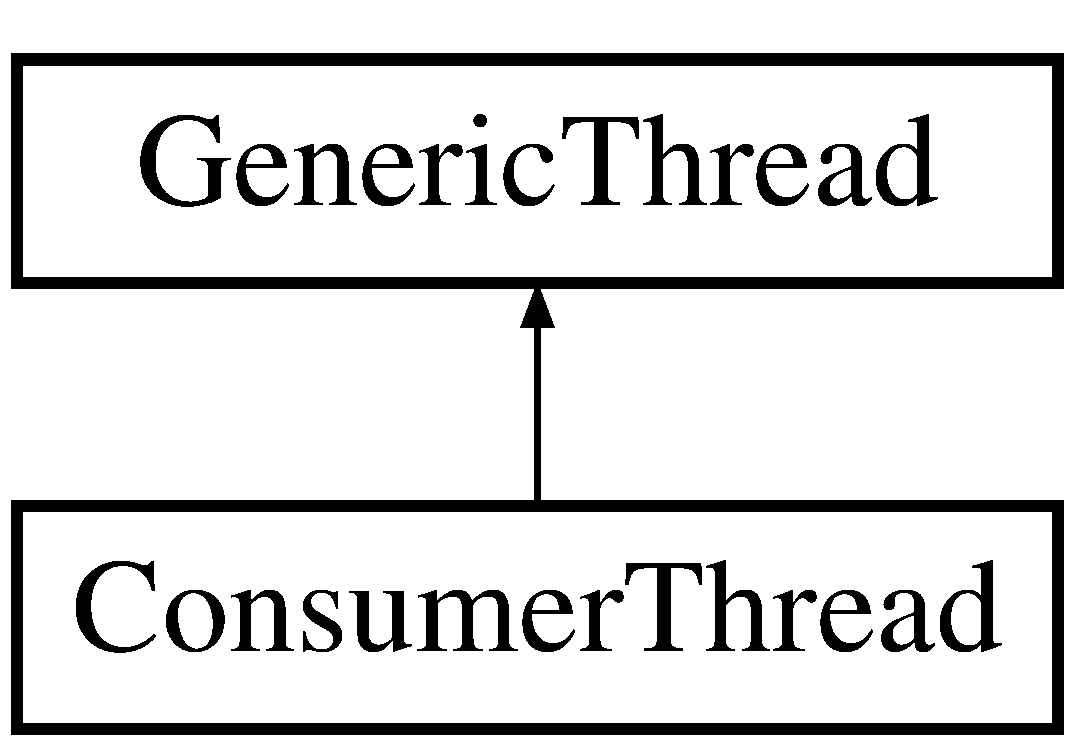
\includegraphics[height=2.000000cm]{classConsumerThread}
\end{center}
\end{figure}
\subsection*{Public Member Functions}
\begin{DoxyCompactItemize}
\item 
\hypertarget{classConsumerThread_a000214667d1ad9d31ce7133f6fbf9aac}{{\bfseries Consumer\-Thread} (\hyperlink{classGenericQueue}{Generic\-Queue}$<$ \hyperlink{classWorkItem}{Work\-Item} $\ast$ $>$ \&queue)}\label{classConsumerThread_a000214667d1ad9d31ce7133f6fbf9aac}

\item 
\hypertarget{classConsumerThread_a8fde7a9b6c2c0b3c62a9fd3c50296557}{void $\ast$ {\bfseries run} ()}\label{classConsumerThread_a8fde7a9b6c2c0b3c62a9fd3c50296557}

\end{DoxyCompactItemize}


The documentation for this class was generated from the following file\-:\begin{DoxyCompactItemize}
\item 
src/store/gqueue.\-cpp\end{DoxyCompactItemize}

\hypertarget{classunit_1_1CosineGen}{}\section{unit\+:\+:Cosine\+Gen Class Reference}
\label{classunit_1_1CosineGen}\index{unit\+::\+Cosine\+Gen@{unit\+::\+Cosine\+Gen}}


{\ttfamily \#include $<$Cosine\+Gen.\+h$>$}

Inheritance diagram for unit\+:\+:Cosine\+Gen\+:\begin{figure}[H]
\begin{center}
\leavevmode
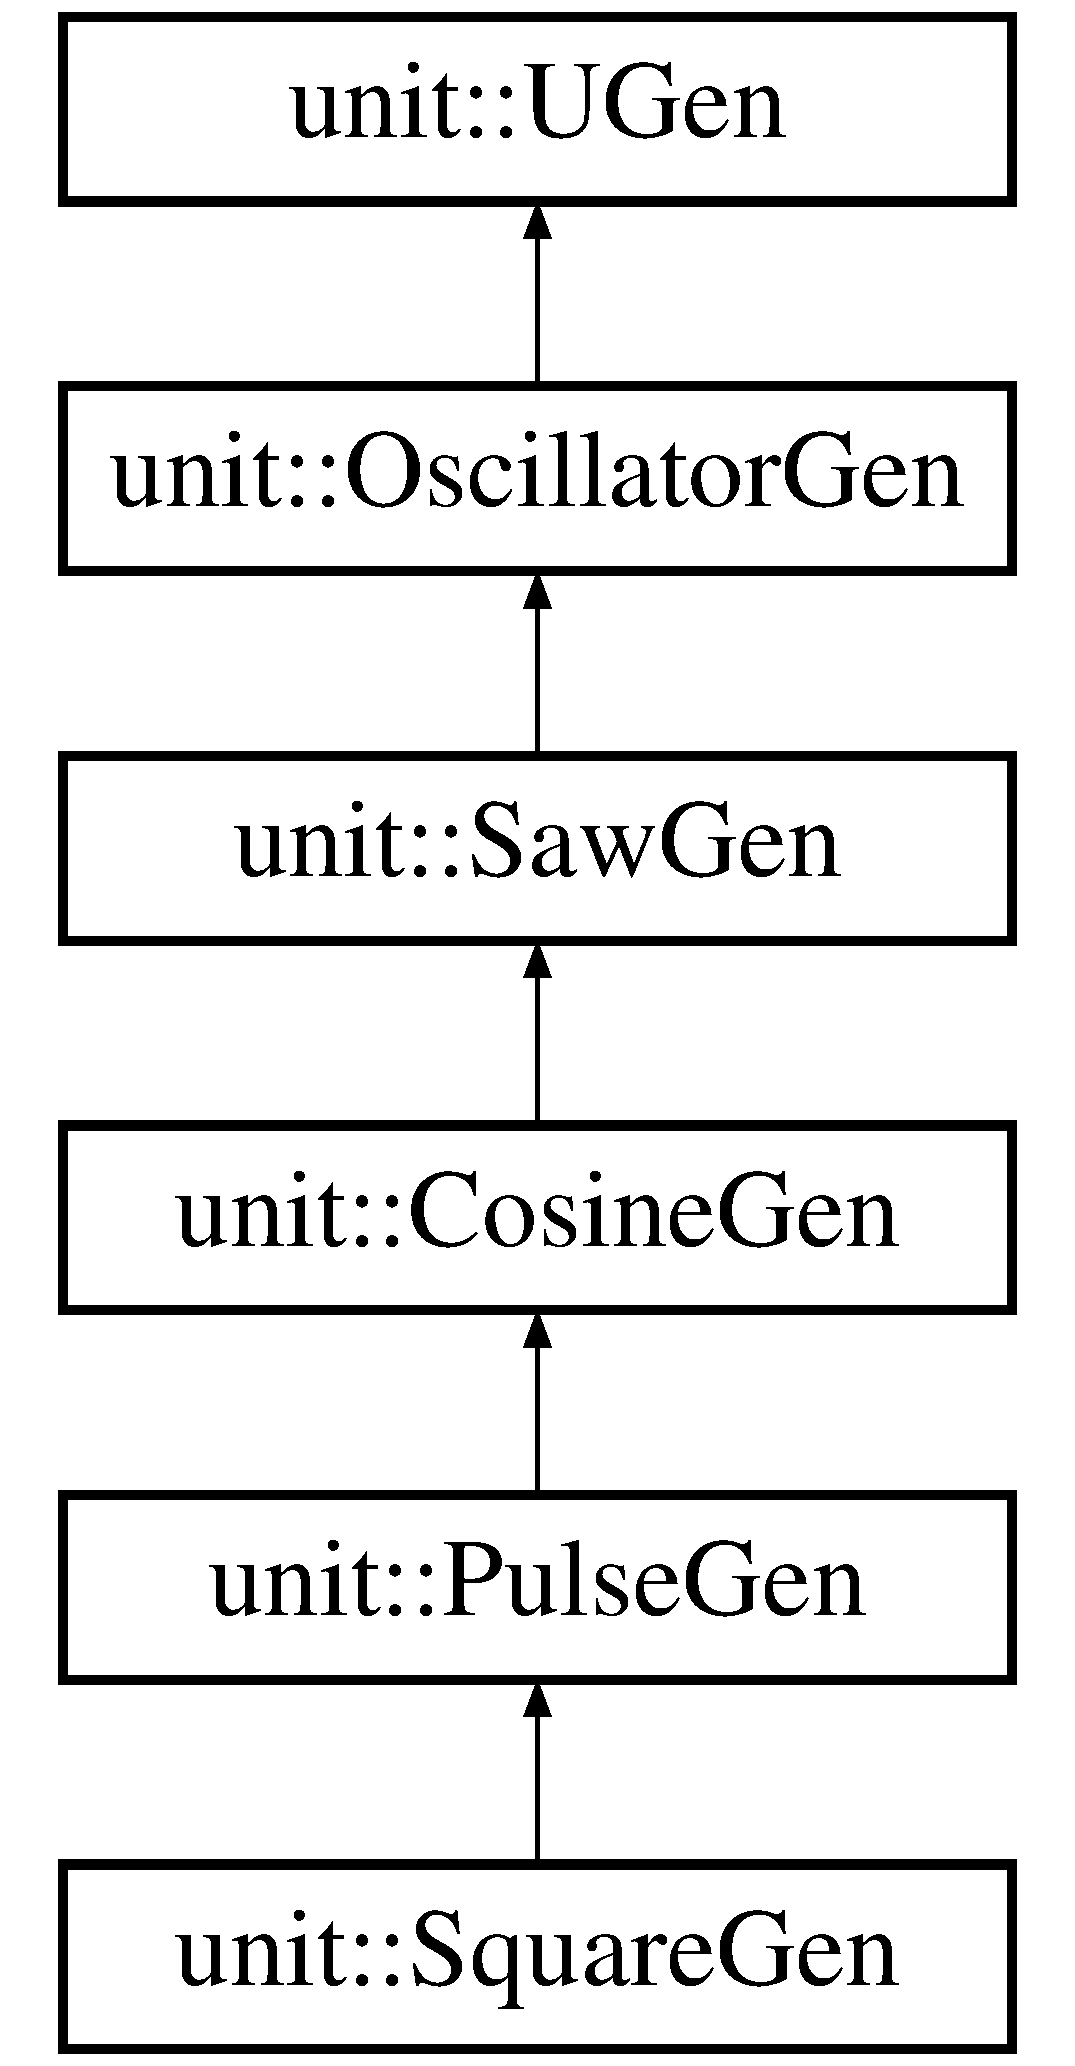
\includegraphics[height=6.000000cm]{classunit_1_1CosineGen}
\end{center}
\end{figure}
\subsection*{Public Member Functions}
\begin{DoxyCompactItemize}
\item 
{\bfseries Cosine\+Gen} (std\+::string name)\hypertarget{classunit_1_1CosineGen_a1eb4aa0471f337e95653d91e550f58cb}{}\label{classunit_1_1CosineGen_a1eb4aa0471f337e95653d91e550f58cb}

\item 
float {\bfseries tick} ()\hypertarget{classunit_1_1CosineGen_a4c1ceffaf70b5eae5c4153ee4b93c001}{}\label{classunit_1_1CosineGen_a4c1ceffaf70b5eae5c4153ee4b93c001}

\item 
void {\bfseries control} (std\+::string port\+Name, float value)\hypertarget{classunit_1_1CosineGen_a15411f97b09516de2bf85327615f1784}{}\label{classunit_1_1CosineGen_a15411f97b09516de2bf85327615f1784}

\item 
void {\bfseries set\+Frequency} (float value)\hypertarget{classunit_1_1CosineGen_aebdf5bbd7a0614f3a3cd2ae0d8602b32}{}\label{classunit_1_1CosineGen_aebdf5bbd7a0614f3a3cd2ae0d8602b32}

\item 
float {\bfseries get\+Frequency} ()\hypertarget{classunit_1_1CosineGen_a2865a158e86e8e85ac2c4d686de65fce}{}\label{classunit_1_1CosineGen_a2865a158e86e8e85ac2c4d686de65fce}

\end{DoxyCompactItemize}
\subsection*{Additional Inherited Members}


\subsection{Detailed Description}
\hyperlink{classunit_1_1CosineGen}{Cosine\+Gen} is generating a cosine wave form based on a cosine wave table.

The saw wave form is transformed into a ramp \mbox{[}0,1\mbox{]} and used as a normalized index into the wave table.

\begin{DoxyAuthor}{Author}
jtm, email\+:  \href{mailto:milde@hs-fulda.de}{\tt milde@hs-\/fulda.\+de} 
\end{DoxyAuthor}
\begin{DoxySince}{Since}
04-\/2016 
\end{DoxySince}
\begin{DoxyVersion}{Version}
1.\+0 
\end{DoxyVersion}


The documentation for this class was generated from the following files\+:\begin{DoxyCompactItemize}
\item 
include/Cosine\+Gen.\+h\item 
unit/Cosine\+Gen.\+cpp\end{DoxyCompactItemize}

\hypertarget{classCosineTable}{}\section{Cosine\+Table Class Reference}
\label{classCosineTable}\index{Cosine\+Table@{Cosine\+Table}}


{\ttfamily \#include $<$Cosine\+Table.\+h$>$}

Inheritance diagram for Cosine\+Table\+:\begin{figure}[H]
\begin{center}
\leavevmode
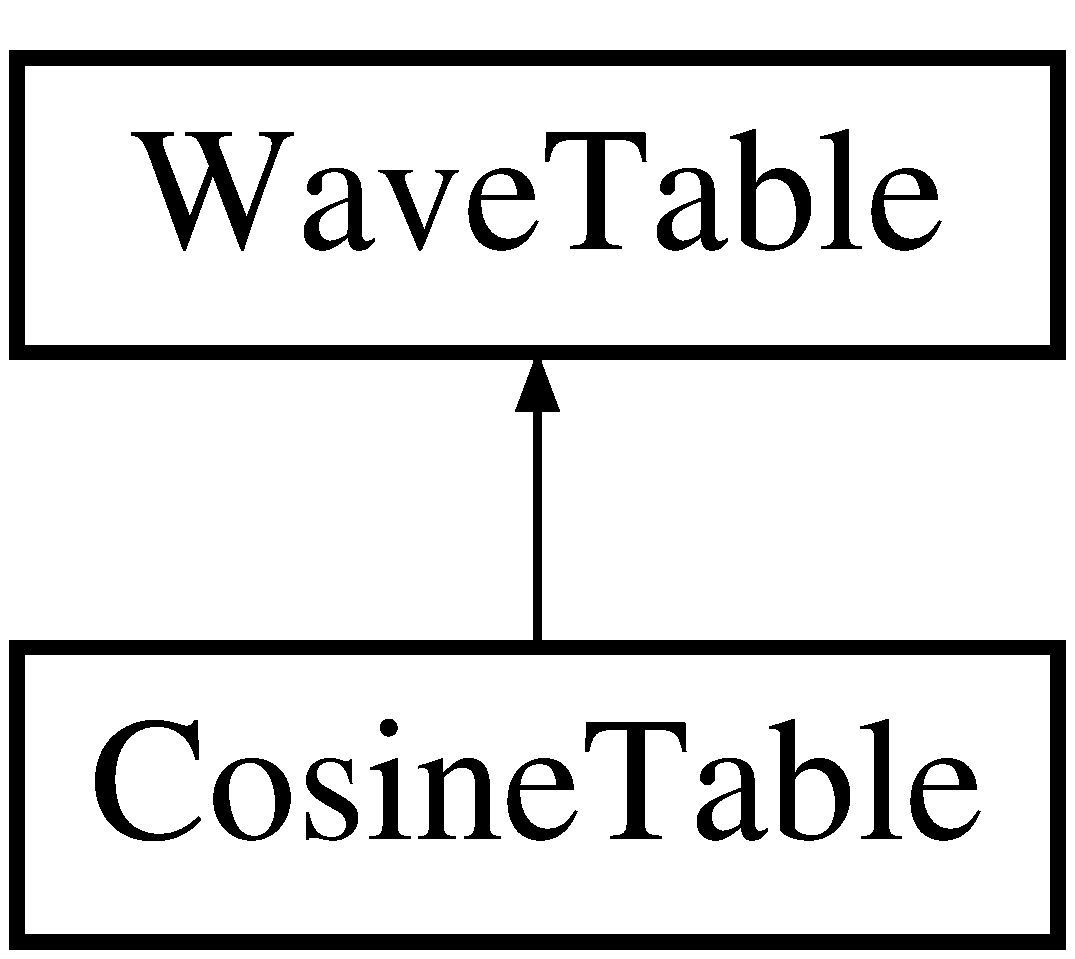
\includegraphics[height=2.000000cm]{classCosineTable}
\end{center}
\end{figure}
\subsection*{Public Member Functions}
\begin{DoxyCompactItemize}
\item 
void {\bfseries init} ()\hypertarget{classCosineTable_aa44f664688eca2ff8de26b2ee5d78785}{}\label{classCosineTable_aa44f664688eca2ff8de26b2ee5d78785}

\end{DoxyCompactItemize}
\subsection*{Additional Inherited Members}


\subsection{Detailed Description}
\hyperlink{classCosineTable}{Cosine\+Table} stores the cosine values for x in \mbox{[}0, 2$\ast$pi\mbox{]}.

Currently no interpolation between values is calculated. The table size is defined for the base class \hyperlink{classWaveTable}{Wave\+Table}.

Access to the values is provided through


\begin{DoxyItemize}
\item {\bfseries get(int idx)}\+: a cyclic integer index, or through
\item {\bfseries get\+Normed\+Idx(float idx)}\+: a cyclic normalized float index in the range \mbox{[}0,1\mbox{]}.
\end{DoxyItemize}

\begin{DoxyAuthor}{Author}
jtm, email\+:  \href{mailto:milde@hs-fulda.de}{\tt milde@hs-\/fulda.\+de} 
\end{DoxyAuthor}
\begin{DoxySince}{Since}
04-\/2016 
\end{DoxySince}
\begin{DoxyVersion}{Version}
1.\+0 
\end{DoxyVersion}


The documentation for this class was generated from the following files\+:\begin{DoxyCompactItemize}
\item 
include/Cosine\+Table.\+h\item 
util/Cosine\+Table.\+cpp\end{DoxyCompactItemize}

\hypertarget{classCONFIG4CPP__NAMESPACE_1_1DefaultSecurity}{\section{C\-O\-N\-F\-I\-G4\-C\-P\-P\-\_\-\-N\-A\-M\-E\-S\-P\-A\-C\-E\-:\-:Default\-Security Class Reference}
\label{classCONFIG4CPP__NAMESPACE_1_1DefaultSecurity}\index{C\-O\-N\-F\-I\-G4\-C\-P\-P\-\_\-\-N\-A\-M\-E\-S\-P\-A\-C\-E\-::\-Default\-Security@{C\-O\-N\-F\-I\-G4\-C\-P\-P\-\_\-\-N\-A\-M\-E\-S\-P\-A\-C\-E\-::\-Default\-Security}}
}
\subsection*{Public Member Functions}
\begin{DoxyCompactItemize}
\item 
\hypertarget{classCONFIG4CPP__NAMESPACE_1_1DefaultSecurity_a58f94dc9791231138cbab14151cc3f0a}{const char $\ast$ {\bfseries get\-String} ()}\label{classCONFIG4CPP__NAMESPACE_1_1DefaultSecurity_a58f94dc9791231138cbab14151cc3f0a}

\end{DoxyCompactItemize}


The documentation for this class was generated from the following files\-:\begin{DoxyCompactItemize}
\item 
src/configuration/config4cpp/src/Default\-Security.\-h\item 
src/configuration/config4cpp/src/Default\-Security.\-cpp\end{DoxyCompactItemize}

\hypertarget{classCONFIG4CPP__NAMESPACE_1_1DefaultSecurityConfiguration}{\section{C\-O\-N\-F\-I\-G4\-C\-P\-P\-\_\-\-N\-A\-M\-E\-S\-P\-A\-C\-E\-:\-:Default\-Security\-Configuration Class Reference}
\label{classCONFIG4CPP__NAMESPACE_1_1DefaultSecurityConfiguration}\index{C\-O\-N\-F\-I\-G4\-C\-P\-P\-\_\-\-N\-A\-M\-E\-S\-P\-A\-C\-E\-::\-Default\-Security\-Configuration@{C\-O\-N\-F\-I\-G4\-C\-P\-P\-\_\-\-N\-A\-M\-E\-S\-P\-A\-C\-E\-::\-Default\-Security\-Configuration}}
}
Inheritance diagram for C\-O\-N\-F\-I\-G4\-C\-P\-P\-\_\-\-N\-A\-M\-E\-S\-P\-A\-C\-E\-:\-:Default\-Security\-Configuration\-:\begin{figure}[H]
\begin{center}
\leavevmode
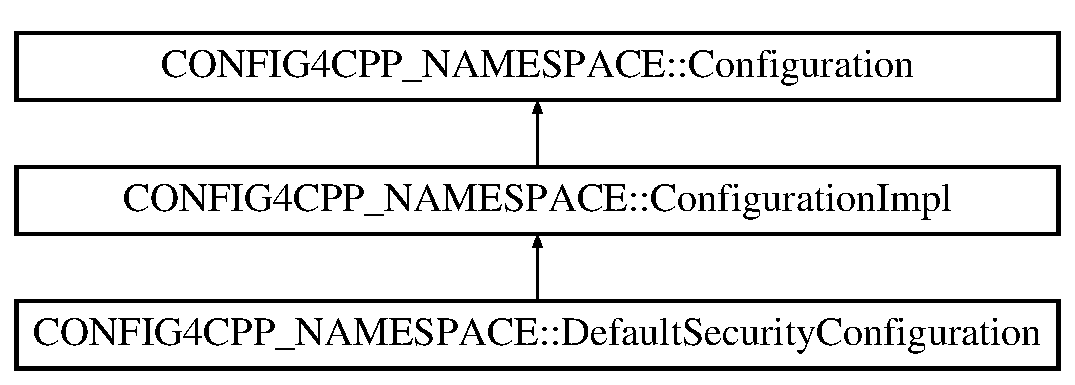
\includegraphics[height=3.000000cm]{classCONFIG4CPP__NAMESPACE_1_1DefaultSecurityConfiguration}
\end{center}
\end{figure}
\subsection*{Static Public Attributes}
\begin{DoxyCompactItemize}
\item 
\hypertarget{classCONFIG4CPP__NAMESPACE_1_1DefaultSecurityConfiguration_a5202578aba39793f8f040c9f9c8f0f69}{static \hyperlink{classCONFIG4CPP__NAMESPACE_1_1DefaultSecurityConfiguration}{Default\-Security\-Configuration} {\bfseries singleton}}\label{classCONFIG4CPP__NAMESPACE_1_1DefaultSecurityConfiguration_a5202578aba39793f8f040c9f9c8f0f69}

\end{DoxyCompactItemize}
\subsection*{Additional Inherited Members}


The documentation for this class was generated from the following files\-:\begin{DoxyCompactItemize}
\item 
src/configuration/config4cpp/src/Default\-Security\-Configuration.\-h\item 
src/configuration/config4cpp/src/Default\-Security\-Configuration.\-cpp\end{DoxyCompactItemize}

\hypertarget{classunit_1_1EGOneStepGen}{\section{unit\-:\-:E\-G\-One\-Step\-Gen Class Reference}
\label{classunit_1_1EGOneStepGen}\index{unit\-::\-E\-G\-One\-Step\-Gen@{unit\-::\-E\-G\-One\-Step\-Gen}}
}


{\ttfamily \#include $<$E\-G\-One\-Step\-Gen.\-h$>$}

Inheritance diagram for unit\-:\-:E\-G\-One\-Step\-Gen\-:\begin{figure}[H]
\begin{center}
\leavevmode
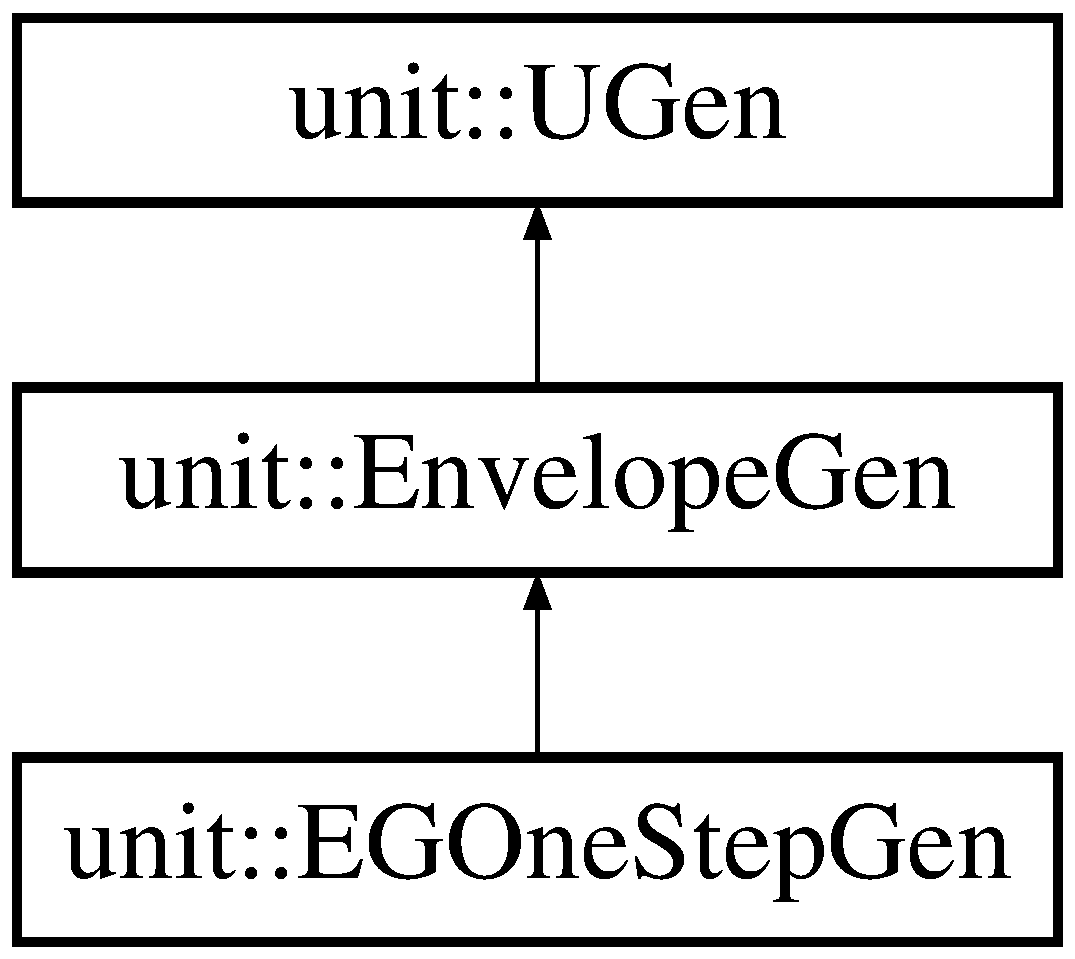
\includegraphics[height=3.000000cm]{classunit_1_1EGOneStepGen}
\end{center}
\end{figure}
\subsection*{Public Member Functions}
\begin{DoxyCompactItemize}
\item 
\hypertarget{classunit_1_1EGOneStepGen_a9bc697acabed6c7b0467369ba073ede1}{{\bfseries E\-G\-One\-Step\-Gen} (std\-::string name)}\label{classunit_1_1EGOneStepGen_a9bc697acabed6c7b0467369ba073ede1}

\item 
\hypertarget{classunit_1_1EGOneStepGen_a74df96649d7a66d19cb33bf9bf13f54a}{float {\bfseries tick} ()}\label{classunit_1_1EGOneStepGen_a74df96649d7a66d19cb33bf9bf13f54a}

\item 
\hypertarget{classunit_1_1EGOneStepGen_a8979594fb226c732a9b8232664f09047}{void {\bfseries control} (std\-::string port\-Name, float value)}\label{classunit_1_1EGOneStepGen_a8979594fb226c732a9b8232664f09047}

\item 
\hypertarget{classunit_1_1EGOneStepGen_ae9f187e0f266559a80e4f4b534d79f78}{bool {\bfseries finished} ()}\label{classunit_1_1EGOneStepGen_ae9f187e0f266559a80e4f4b534d79f78}

\item 
\hypertarget{classunit_1_1EGOneStepGen_af94a0976e166a3f53b7bf14de58f81d6}{void {\bfseries set\-Trigger} ()}\label{classunit_1_1EGOneStepGen_af94a0976e166a3f53b7bf14de58f81d6}

\item 
\hypertarget{classunit_1_1EGOneStepGen_aaf02138e168cad06cb955944f57ce93c}{void {\bfseries set\-Duration} (float seconds)}\label{classunit_1_1EGOneStepGen_aaf02138e168cad06cb955944f57ce93c}

\item 
\hypertarget{classunit_1_1EGOneStepGen_af2b5bd8522fac9dc997d78d3750cdbbb}{void {\bfseries set\-Start\-Level} (float level)}\label{classunit_1_1EGOneStepGen_af2b5bd8522fac9dc997d78d3750cdbbb}

\item 
\hypertarget{classunit_1_1EGOneStepGen_a3d58403aa5bebffeaf3f326855e0a233}{void {\bfseries set\-End\-Level} (float level)}\label{classunit_1_1EGOneStepGen_a3d58403aa5bebffeaf3f326855e0a233}

\item 
\hypertarget{classunit_1_1EGOneStepGen_a4898b08a0687e03802abdb7945708cab}{void {\bfseries reset} ()}\label{classunit_1_1EGOneStepGen_a4898b08a0687e03802abdb7945708cab}

\end{DoxyCompactItemize}
\subsection*{Additional Inherited Members}


\subsection{Detailed Description}
\hyperlink{classunit_1_1EGOneStepGen}{E\-G\-One\-Step\-Gen} is providing a linear interpolation based on the current time step.

\begin{DoxyAuthor}{Author}
jtm 
\end{DoxyAuthor}
\begin{DoxySince}{Since}
04-\/2016 
\end{DoxySince}
\begin{DoxyVersion}{Version}
1.\-0 
\end{DoxyVersion}


The documentation for this class was generated from the following files\-:\begin{DoxyCompactItemize}
\item 
src/include/E\-G\-One\-Step\-Gen.\-h\item 
src/unit/E\-G\-One\-Step\-Gen.\-cpp\end{DoxyCompactItemize}

\hypertarget{classunit_1_1EGUpDownGen}{}\section{unit\+:\+:E\+G\+Up\+Down\+Gen Class Reference}
\label{classunit_1_1EGUpDownGen}\index{unit\+::\+E\+G\+Up\+Down\+Gen@{unit\+::\+E\+G\+Up\+Down\+Gen}}


{\ttfamily \#include $<$E\+G\+Up\+Down\+Gen.\+h$>$}

Inheritance diagram for unit\+:\+:E\+G\+Up\+Down\+Gen\+:\begin{figure}[H]
\begin{center}
\leavevmode
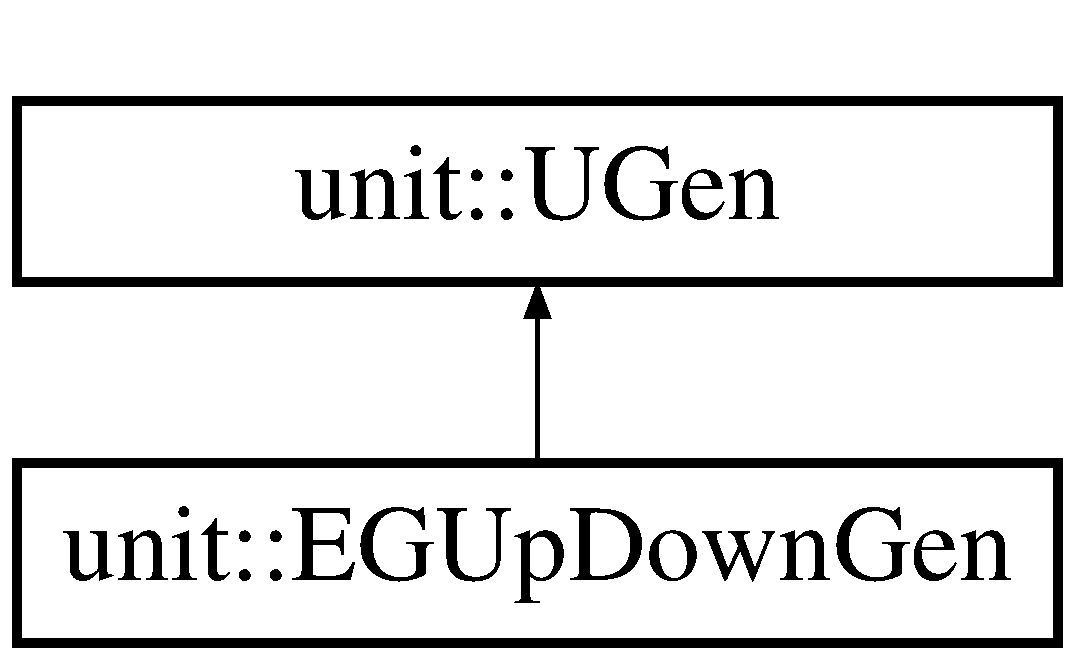
\includegraphics[height=3.000000cm]{classunit_1_1EGUpDownGen}
\end{center}
\end{figure}
\subsection*{Public Member Functions}
\begin{DoxyCompactItemize}
\item 
{\bfseries E\+G\+Up\+Down\+Gen} (std\+::string name)\hypertarget{classunit_1_1EGUpDownGen_abc35a572da36fa26f4b54beabfc6268e}{}\label{classunit_1_1EGUpDownGen_abc35a572da36fa26f4b54beabfc6268e}

\item 
float {\bfseries tick} ()\hypertarget{classunit_1_1EGUpDownGen_abea11de5389345064a8395d54411e3b3}{}\label{classunit_1_1EGUpDownGen_abea11de5389345064a8395d54411e3b3}

\item 
void {\bfseries control} (std\+::string port\+Name, float value)\hypertarget{classunit_1_1EGUpDownGen_ac1ef59d9023034c17b46e09bfae15178}{}\label{classunit_1_1EGUpDownGen_ac1ef59d9023034c17b46e09bfae15178}

\end{DoxyCompactItemize}
\subsection*{Additional Inherited Members}


\subsection{Detailed Description}
\hyperlink{classunit_1_1EGUpDownGen}{E\+G\+Up\+Down\+Gen} generates a simple symetrical up/down envelope.

\begin{DoxyAuthor}{Author}
jtm, email\+:  \href{mailto:milde@hs-fulda.de}{\tt milde@hs-\/fulda.\+de} 
\end{DoxyAuthor}
\begin{DoxySince}{Since}
04-\/2016 
\end{DoxySince}
\begin{DoxyVersion}{Version}
1.\+0 
\end{DoxyVersion}


The documentation for this class was generated from the following files\+:\begin{DoxyCompactItemize}
\item 
include/E\+G\+Up\+Down\+Gen.\+h\item 
unit/E\+G\+Up\+Down\+Gen.\+cpp\end{DoxyCompactItemize}

\hypertarget{structCONFIG4CPP__NAMESPACE_1_1EnumNameAndValue}{\section{C\-O\-N\-F\-I\-G4\-C\-P\-P\-\_\-\-N\-A\-M\-E\-S\-P\-A\-C\-E\-:\-:Enum\-Name\-And\-Value Struct Reference}
\label{structCONFIG4CPP__NAMESPACE_1_1EnumNameAndValue}\index{C\-O\-N\-F\-I\-G4\-C\-P\-P\-\_\-\-N\-A\-M\-E\-S\-P\-A\-C\-E\-::\-Enum\-Name\-And\-Value@{C\-O\-N\-F\-I\-G4\-C\-P\-P\-\_\-\-N\-A\-M\-E\-S\-P\-A\-C\-E\-::\-Enum\-Name\-And\-Value}}
}
\subsection*{Public Attributes}
\begin{DoxyCompactItemize}
\item 
\hypertarget{structCONFIG4CPP__NAMESPACE_1_1EnumNameAndValue_ab0b063367b99272bd3f89ec9f6a4fb3a}{const char $\ast$ {\bfseries name}}\label{structCONFIG4CPP__NAMESPACE_1_1EnumNameAndValue_ab0b063367b99272bd3f89ec9f6a4fb3a}

\item 
\hypertarget{structCONFIG4CPP__NAMESPACE_1_1EnumNameAndValue_a57c91cbbf43ccbe27898c9d7755875aa}{int {\bfseries value}}\label{structCONFIG4CPP__NAMESPACE_1_1EnumNameAndValue_a57c91cbbf43ccbe27898c9d7755875aa}

\end{DoxyCompactItemize}


The documentation for this struct was generated from the following file\-:\begin{DoxyCompactItemize}
\item 
src/configuration/config4cpp/include/config4cpp/Configuration.\-h\end{DoxyCompactItemize}

\hypertarget{classunit_1_1EnvelopeGen}{}\section{unit\+:\+:Envelope\+Gen Class Reference}
\label{classunit_1_1EnvelopeGen}\index{unit\+::\+Envelope\+Gen@{unit\+::\+Envelope\+Gen}}
Inheritance diagram for unit\+:\+:Envelope\+Gen\+:\begin{figure}[H]
\begin{center}
\leavevmode
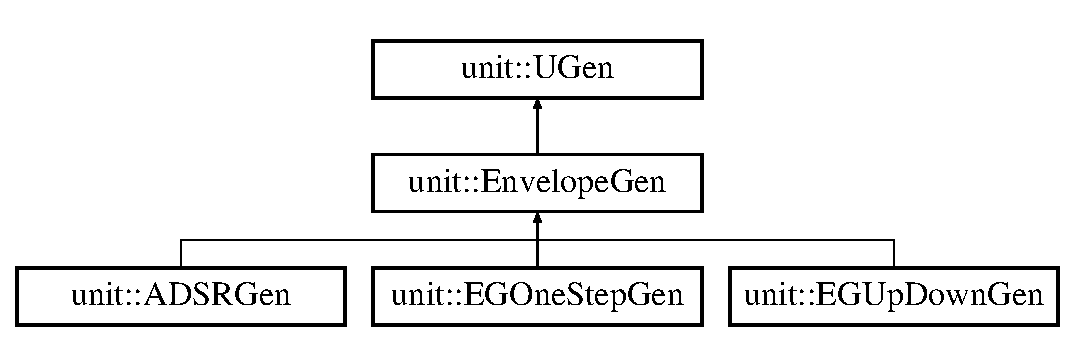
\includegraphics[height=3.000000cm]{classunit_1_1EnvelopeGen}
\end{center}
\end{figure}
\subsection*{Public Member Functions}
\begin{DoxyCompactItemize}
\item 
{\bfseries Envelope\+Gen} (std\+::string name)\hypertarget{classunit_1_1EnvelopeGen_a2925f305c08e3316c3b1cbdabea03bde}{}\label{classunit_1_1EnvelopeGen_a2925f305c08e3316c3b1cbdabea03bde}

\end{DoxyCompactItemize}
\subsection*{Additional Inherited Members}


The documentation for this class was generated from the following files\+:\begin{DoxyCompactItemize}
\item 
include/Envelope\+Gen.\+h\item 
unit/Envelope\+Gen.\+cpp\end{DoxyCompactItemize}

\hypertarget{classExamplePacketListener}{}\section{Example\+Packet\+Listener Class Reference}
\label{classExamplePacketListener}\index{Example\+Packet\+Listener@{Example\+Packet\+Listener}}
Inheritance diagram for Example\+Packet\+Listener\+:\begin{figure}[H]
\begin{center}
\leavevmode
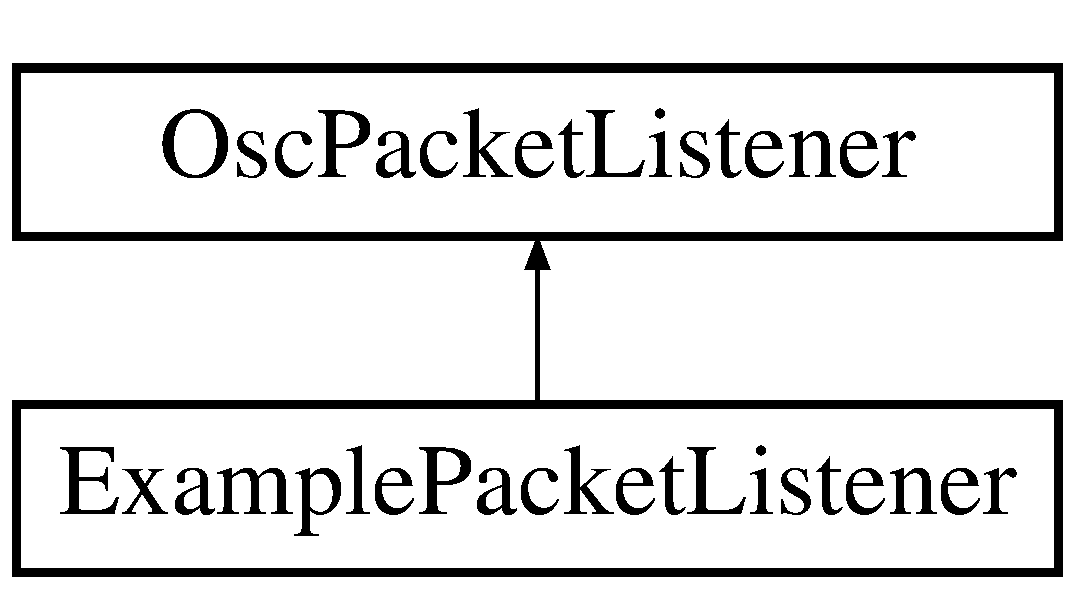
\includegraphics[height=2.000000cm]{classExamplePacketListener}
\end{center}
\end{figure}
\subsection*{Protected Member Functions}
\begin{DoxyCompactItemize}
\item 
virtual void {\bfseries Process\+Message} (const osc\+::\+Received\+Message \&m, const Ip\+Endpoint\+Name \&remote\+Endpoint)\hypertarget{classExamplePacketListener_a688ed2a3ec01d0fb7661f4fe0ffc90df}{}\label{classExamplePacketListener_a688ed2a3ec01d0fb7661f4fe0ffc90df}

\end{DoxyCompactItemize}


The documentation for this class was generated from the following file\+:\begin{DoxyCompactItemize}
\item 
Simple\+Receive.\+cpp\end{DoxyCompactItemize}

\hypertarget{structCONFIG4CPP__NAMESPACE_1_1LexBase_1_1FuncInfo}{\section{C\-O\-N\-F\-I\-G4\-C\-P\-P\-\_\-\-N\-A\-M\-E\-S\-P\-A\-C\-E\-:\-:Lex\-Base\-:\-:Func\-Info Struct Reference}
\label{structCONFIG4CPP__NAMESPACE_1_1LexBase_1_1FuncInfo}\index{C\-O\-N\-F\-I\-G4\-C\-P\-P\-\_\-\-N\-A\-M\-E\-S\-P\-A\-C\-E\-::\-Lex\-Base\-::\-Func\-Info@{C\-O\-N\-F\-I\-G4\-C\-P\-P\-\_\-\-N\-A\-M\-E\-S\-P\-A\-C\-E\-::\-Lex\-Base\-::\-Func\-Info}}
}
\subsection*{Public Attributes}
\begin{DoxyCompactItemize}
\item 
\hypertarget{structCONFIG4CPP__NAMESPACE_1_1LexBase_1_1FuncInfo_ad9997846f15ca406d44a8ef3672c575d}{const char $\ast$ {\bfseries m\-\_\-spelling}}\label{structCONFIG4CPP__NAMESPACE_1_1LexBase_1_1FuncInfo_ad9997846f15ca406d44a8ef3672c575d}

\item 
\hypertarget{structCONFIG4CPP__NAMESPACE_1_1LexBase_1_1FuncInfo_a82bf928293b95f6a1c6176a543246a9e}{short {\bfseries m\-\_\-func\-Type}}\label{structCONFIG4CPP__NAMESPACE_1_1LexBase_1_1FuncInfo_a82bf928293b95f6a1c6176a543246a9e}

\item 
\hypertarget{structCONFIG4CPP__NAMESPACE_1_1LexBase_1_1FuncInfo_a6d5df6ba6b0142701fc9cd41849973a3}{short {\bfseries m\-\_\-symbol}}\label{structCONFIG4CPP__NAMESPACE_1_1LexBase_1_1FuncInfo_a6d5df6ba6b0142701fc9cd41849973a3}

\end{DoxyCompactItemize}


The documentation for this struct was generated from the following file\-:\begin{DoxyCompactItemize}
\item 
src/configuration/config4cpp/src/Lex\-Base.\-h\end{DoxyCompactItemize}

\hypertarget{classunit_1_1GatedConstantGen}{}\section{unit\+:\+:Gated\+Constant\+Gen Class Reference}
\label{classunit_1_1GatedConstantGen}\index{unit\+::\+Gated\+Constant\+Gen@{unit\+::\+Gated\+Constant\+Gen}}
Inheritance diagram for unit\+:\+:Gated\+Constant\+Gen\+:\begin{figure}[H]
\begin{center}
\leavevmode
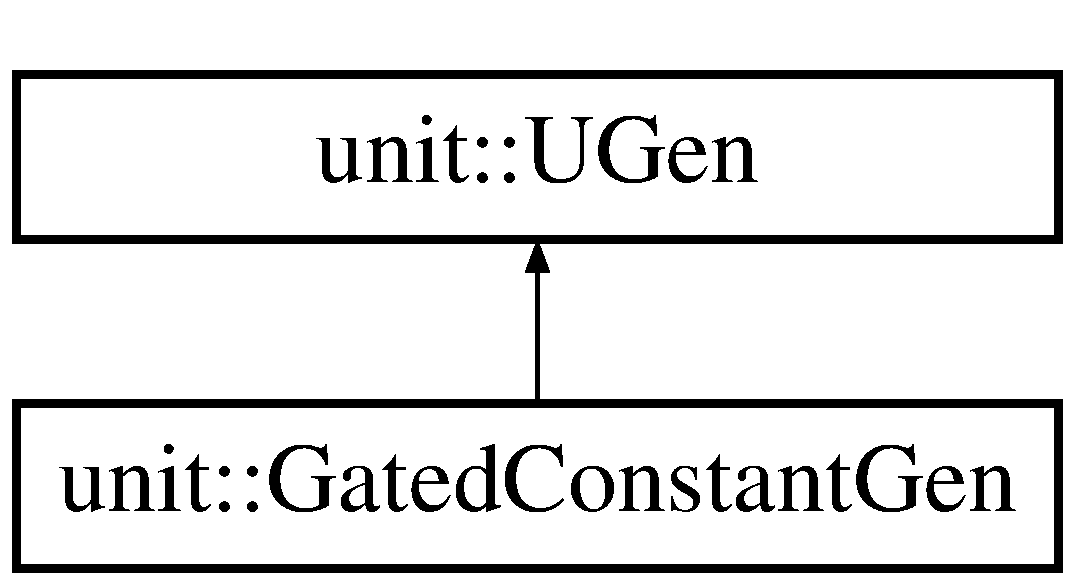
\includegraphics[height=2.000000cm]{classunit_1_1GatedConstantGen}
\end{center}
\end{figure}
\subsection*{Public Member Functions}
\begin{DoxyCompactItemize}
\item 
{\bfseries Gated\+Constant\+Gen} (std\+::string name)\hypertarget{classunit_1_1GatedConstantGen_ad30ad26411f421228c8f7075b4d27f9a}{}\label{classunit_1_1GatedConstantGen_ad30ad26411f421228c8f7075b4d27f9a}

\item 
void {\bfseries control} (std\+::string port\+Name, float value)\hypertarget{classunit_1_1GatedConstantGen_a8365ddc2a6ddebc86e196fa381a5648d}{}\label{classunit_1_1GatedConstantGen_a8365ddc2a6ddebc86e196fa381a5648d}

\item 
float {\bfseries tick} ()\hypertarget{classunit_1_1GatedConstantGen_aafff659359fed9f28c703acd0076c081}{}\label{classunit_1_1GatedConstantGen_aafff659359fed9f28c703acd0076c081}

\end{DoxyCompactItemize}
\subsection*{Additional Inherited Members}


The documentation for this class was generated from the following files\+:\begin{DoxyCompactItemize}
\item 
unit/Gated\+Constant\+Gen.\+h\item 
unit/Gated\+Constant\+Gen.\+cpp\end{DoxyCompactItemize}

\hypertarget{classGenericQueue}{\section{Generic\-Queue$<$ T $>$ Class Template Reference}
\label{classGenericQueue}\index{Generic\-Queue$<$ T $>$@{Generic\-Queue$<$ T $>$}}
}
\subsection*{Public Member Functions}
\begin{DoxyCompactItemize}
\item 
\hypertarget{classGenericQueue_af5de20e93f3ee8d1fdd38a8ec1ae52f6}{void {\bfseries add} (T item)}\label{classGenericQueue_af5de20e93f3ee8d1fdd38a8ec1ae52f6}

\item 
\hypertarget{classGenericQueue_a15366cdc3234d238c664c82524f14c0b}{T {\bfseries remove} ()}\label{classGenericQueue_a15366cdc3234d238c664c82524f14c0b}

\item 
\hypertarget{classGenericQueue_aa94c712ca621ef5c121cd4f9c9188f67}{int {\bfseries size} ()}\label{classGenericQueue_aa94c712ca621ef5c121cd4f9c9188f67}

\item 
\hypertarget{classGenericQueue_a0fd02ceeecaf5c0903e3ee7199b183bc}{void {\bfseries clear} ()}\label{classGenericQueue_a0fd02ceeecaf5c0903e3ee7199b183bc}

\end{DoxyCompactItemize}


The documentation for this class was generated from the following file\-:\begin{DoxyCompactItemize}
\item 
src/include/Generic\-Queue.\-h\end{DoxyCompactItemize}

\hypertarget{classGenericThread}{}\section{Generic\+Thread Class Reference}
\label{classGenericThread}\index{Generic\+Thread@{Generic\+Thread}}
Inheritance diagram for Generic\+Thread\+:\begin{figure}[H]
\begin{center}
\leavevmode
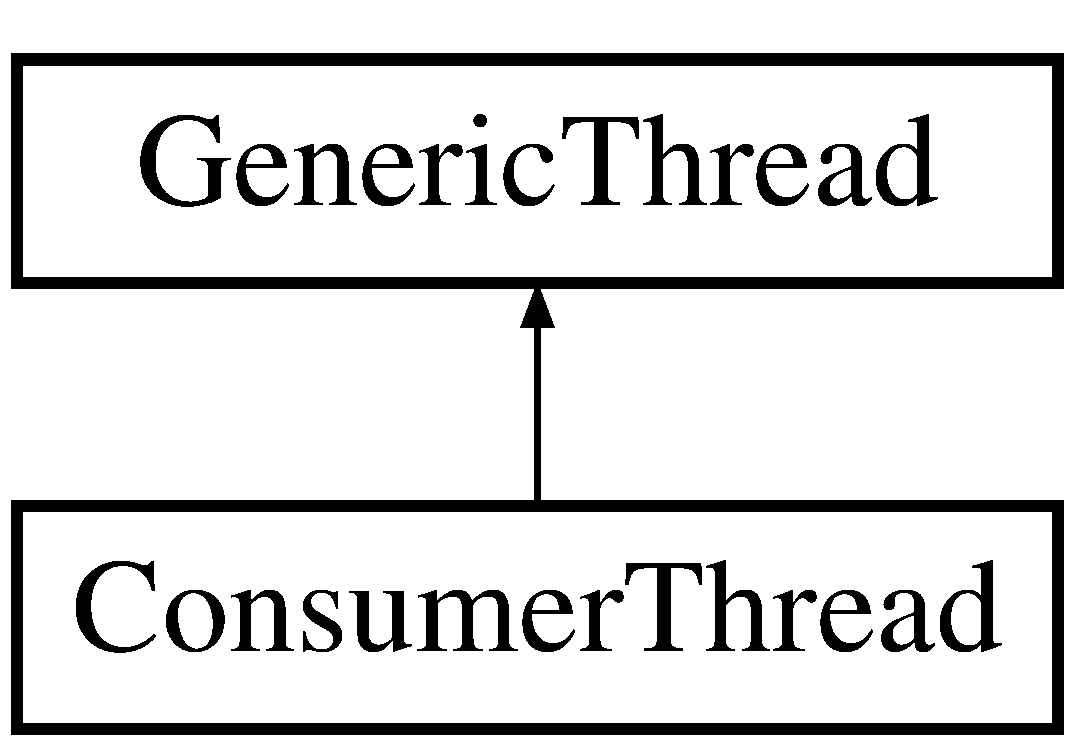
\includegraphics[height=2.000000cm]{classGenericThread}
\end{center}
\end{figure}
\subsection*{Public Member Functions}
\begin{DoxyCompactItemize}
\item 
int {\bfseries start} ()\hypertarget{classGenericThread_ac1d8c3d7dcaae01e89c69093a065141f}{}\label{classGenericThread_ac1d8c3d7dcaae01e89c69093a065141f}

\item 
int {\bfseries join} ()\hypertarget{classGenericThread_a217ef41077ae00ce48372c03838af96a}{}\label{classGenericThread_a217ef41077ae00ce48372c03838af96a}

\item 
int {\bfseries detach} ()\hypertarget{classGenericThread_abd0849015ec4004b789aa3181853fbf6}{}\label{classGenericThread_abd0849015ec4004b789aa3181853fbf6}

\item 
pthread\+\_\+t {\bfseries self} ()\hypertarget{classGenericThread_a0ac1c8aa0c6f5d47d73626c13854d444}{}\label{classGenericThread_a0ac1c8aa0c6f5d47d73626c13854d444}

\item 
virtual void $\ast$ {\bfseries run} ()=0\hypertarget{classGenericThread_a54147ff9f16e7985e634b5f0d6d5b7f9}{}\label{classGenericThread_a54147ff9f16e7985e634b5f0d6d5b7f9}

\end{DoxyCompactItemize}


The documentation for this class was generated from the following files\+:\begin{DoxyCompactItemize}
\item 
store/Generic\+Thread.\+h\item 
store/Generic\+Thread.\+cpp\end{DoxyCompactItemize}

\hypertarget{classGUI}{}\section{G\+UI Class Reference}
\label{classGUI}\index{G\+UI@{G\+UI}}
Inheritance diagram for G\+UI\+:\begin{figure}[H]
\begin{center}
\leavevmode
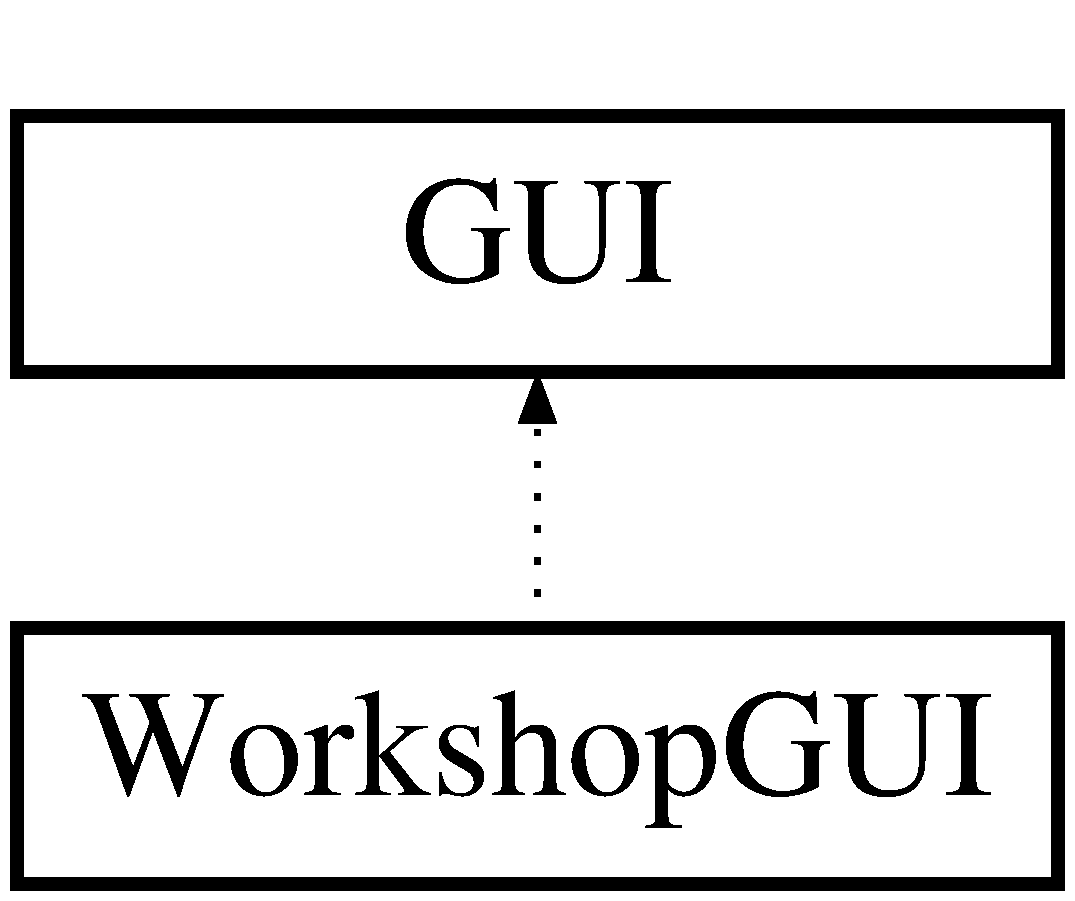
\includegraphics[height=2.000000cm]{classGUI}
\end{center}
\end{figure}
\subsection*{Public Member Functions}
\begin{DoxyCompactItemize}
\item 
virtual void {\bfseries set\+Value} (std\+::string name, float value)\hypertarget{classGUI_ac7565b952201756e1dc1f0b9486f6b28}{}\label{classGUI_ac7565b952201756e1dc1f0b9486f6b28}

\item 
virtual void {\bfseries redraw} ()\hypertarget{classGUI_a86c7f4b8bd81b4c0e191b40a134e2f9e}{}\label{classGUI_a86c7f4b8bd81b4c0e191b40a134e2f9e}

\end{DoxyCompactItemize}


The documentation for this class was generated from the following files\+:\begin{DoxyCompactItemize}
\item 
gui/G\+U\+I.\+h\item 
gui/G\+U\+I.\+cpp\end{DoxyCompactItemize}

\hypertarget{classGUIMapping}{\section{G\-U\-I\-Mapping Class Reference}
\label{classGUIMapping}\index{G\-U\-I\-Mapping@{G\-U\-I\-Mapping}}
}


{\ttfamily \#include $<$G\-U\-I\-Mapping.\-h$>$}

\subsection*{Static Public Member Functions}
\begin{DoxyCompactItemize}
\item 
\hypertarget{classGUIMapping_afc4d931e878ba22a7530d39c66c3a966}{static std\-::string {\bfseries map\-Mini\-Lab2\-Workshop} (int key, int value)}\label{classGUIMapping_afc4d931e878ba22a7530d39c66c3a966}

\end{DoxyCompactItemize}


\subsection{Detailed Description}
\hyperlink{classGUIMapping}{G\-U\-I\-Mapping} maps the part of the Arturia Minilab key, knob, pad and slider codes to control strings used in the ncurses version of the Workshop \hyperlink{classWorkshopGUI}{Workshop\-G\-U\-I}.

\begin{DoxyAuthor}{Author}
jtm, email\-:  \href{mailto:milde@hs-fulda.de}{\tt milde@hs-\/fulda.\-de} 
\end{DoxyAuthor}
\begin{DoxySince}{Since}
04-\/2016 
\end{DoxySince}
\begin{DoxyVersion}{Version}
1.\-0 
\end{DoxyVersion}


The documentation for this class was generated from the following files\-:\begin{DoxyCompactItemize}
\item 
src/include/G\-U\-I\-Mapping.\-h\item 
src/gui/G\-U\-I\-Mapping.\-cpp\end{DoxyCompactItemize}

\hypertarget{classIDGenerator}{\section{I\-D\-Generator Class Reference}
\label{classIDGenerator}\index{I\-D\-Generator@{I\-D\-Generator}}
}
\subsection*{Public Member Functions}
\begin{DoxyCompactItemize}
\item 
\hypertarget{classIDGenerator_a223bf057a0ad9e69df527142dfe1e91b}{std\-::string {\bfseries next\-I\-D} ()}\label{classIDGenerator_a223bf057a0ad9e69df527142dfe1e91b}

\end{DoxyCompactItemize}


The documentation for this class was generated from the following files\-:\begin{DoxyCompactItemize}
\item 
include/I\-D\-Generator.\-h\item 
util/I\-D\-Generator.\-cpp\end{DoxyCompactItemize}

\hypertarget{classInterpolation}{}\section{Interpolation Class Reference}
\label{classInterpolation}\index{Interpolation@{Interpolation}}


{\ttfamily \#include $<$Interpolation.\+h$>$}

\subsection*{Static Public Member Functions}
\begin{DoxyCompactItemize}
\item 
static float {\bfseries map} (float value, float s1, float e1, float s2, float e2)\hypertarget{classInterpolation_adfd3003c39c40ec76342274c65017761}{}\label{classInterpolation_adfd3003c39c40ec76342274c65017761}

\item 
static float {\bfseries map} (int value, int s1, int e1, float s2, float e2)\hypertarget{classInterpolation_ac6eab12deb9f79b79200aad3b219e7c3}{}\label{classInterpolation_ac6eab12deb9f79b79200aad3b219e7c3}

\item 
static int {\bfseries discrete} (float value, float s1, float e1, int max)\hypertarget{classInterpolation_a246c72a835822b7674758d657ed44230}{}\label{classInterpolation_a246c72a835822b7674758d657ed44230}

\item 
static float \hyperlink{classInterpolation_a5549f8859f14153da891222a8ff1a22f}{maplog} (float value, float s1, float e1, float s2, float e2)
\item 
static float {\bfseries mapexp} (float value, float s1, float e1, float s2, float e2)\hypertarget{classInterpolation_a08d1fe5e82708ab26a019e9ae9f851c8}{}\label{classInterpolation_a08d1fe5e82708ab26a019e9ae9f851c8}

\end{DoxyCompactItemize}


\subsection{Detailed Description}
\hyperlink{classInterpolation}{Interpolation} provides a number of helper function to easily calculate the linear interpolation of a value.

\begin{DoxyAuthor}{Author}
jtm 
\end{DoxyAuthor}
\begin{DoxySince}{Since}
04-\/2016 
\end{DoxySince}
\begin{DoxyVersion}{Version}
1.\+0 
\end{DoxyVersion}


\subsection{Member Function Documentation}
\index{Interpolation@{Interpolation}!maplog@{maplog}}
\index{maplog@{maplog}!Interpolation@{Interpolation}}
\subsubsection[{\texorpdfstring{maplog(float value, float s1, float e1, float s2, float e2)}{maplog(float value, float s1, float e1, float s2, float e2)}}]{\setlength{\rightskip}{0pt plus 5cm}float Interpolation\+::maplog (
\begin{DoxyParamCaption}
\item[{float}]{value, }
\item[{float}]{s1, }
\item[{float}]{e1, }
\item[{float}]{s2, }
\item[{float}]{e2}
\end{DoxyParamCaption}
)\hspace{0.3cm}{\ttfamily [static]}}\hypertarget{classInterpolation_a5549f8859f14153da891222a8ff1a22f}{}\label{classInterpolation_a5549f8859f14153da891222a8ff1a22f}
Calculates the logarithm() of the linear mapping of the input value from interval \mbox{[}s1,e1\mbox{]} to interval \mbox{[}s2,e2\mbox{]}.


\begin{DoxyItemize}
\item The logarithmic result allows for a more fine grained control of the {\bfseries higher} end of the interval.
\item The result should be normalized by dividing the result by log(e2-\/s2).
\end{DoxyItemize}

\begin{DoxyReturn}{Returns}
The log() of the linear mapping.
\end{DoxyReturn}

\begin{DoxyParams}{Parameters}
{\em value} & the value to be mapped (e.\+g. a knob value) \\
\hline
{\em s1} & start of domain interval \\
\hline
{\em e1} & end of domain interval \\
\hline
{\em s2} & start of range interval \\
\hline
{\em e2} & end of range interval \\
\hline
\end{DoxyParams}


The documentation for this class was generated from the following files\+:\begin{DoxyCompactItemize}
\item 
include/Interpolation.\+h\item 
util/Interpolation.\+cpp\end{DoxyCompactItemize}

\hypertarget{classunit_1_1InvertGen}{}\section{unit\+:\+:Invert\+Gen Class Reference}
\label{classunit_1_1InvertGen}\index{unit\+::\+Invert\+Gen@{unit\+::\+Invert\+Gen}}


{\ttfamily \#include $<$Invert\+Gen.\+h$>$}

Inheritance diagram for unit\+:\+:Invert\+Gen\+:\begin{figure}[H]
\begin{center}
\leavevmode
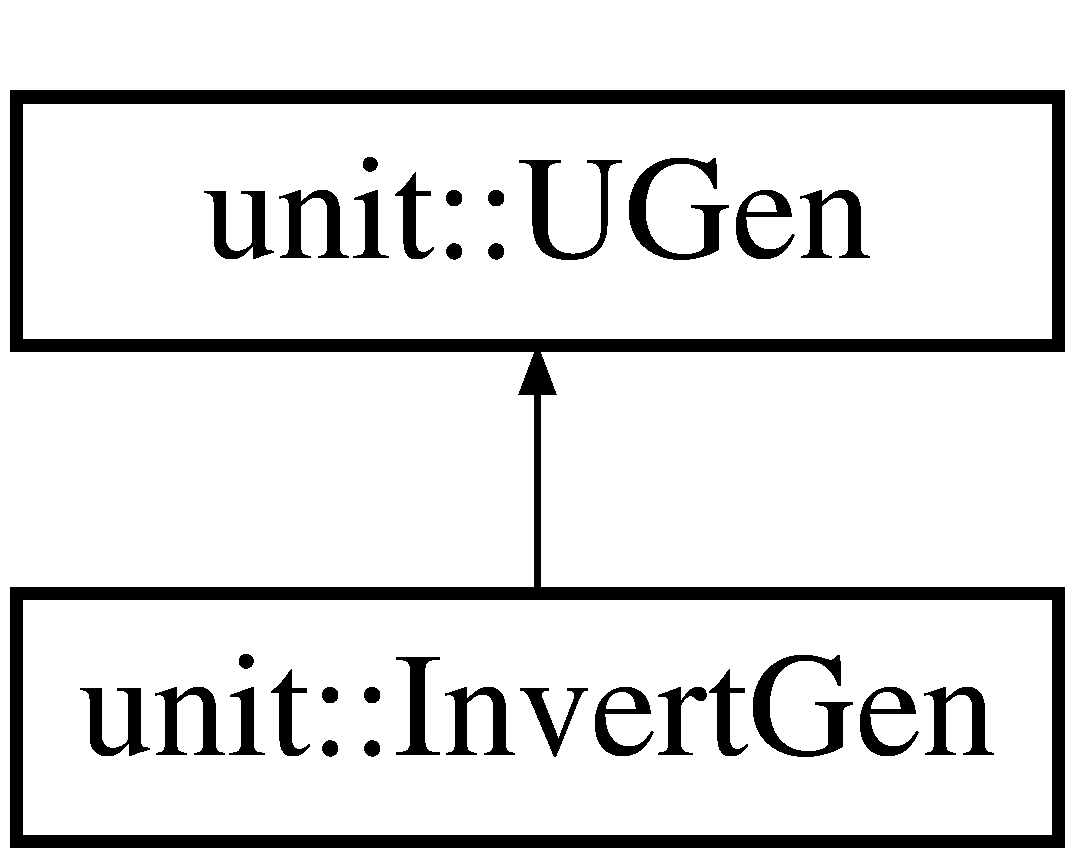
\includegraphics[height=2.000000cm]{classunit_1_1InvertGen}
\end{center}
\end{figure}
\subsection*{Public Member Functions}
\begin{DoxyCompactItemize}
\item 
{\bfseries Invert\+Gen} (std\+::string name)\hypertarget{classunit_1_1InvertGen_a6df9413e609ffe377f728d38c9107f97}{}\label{classunit_1_1InvertGen_a6df9413e609ffe377f728d38c9107f97}

\item 
void {\bfseries control} (std\+::string port\+Name, float value)\hypertarget{classunit_1_1InvertGen_a7f239d73ca02d40f4e2cda336887a852}{}\label{classunit_1_1InvertGen_a7f239d73ca02d40f4e2cda336887a852}

\item 
float {\bfseries tick} ()\hypertarget{classunit_1_1InvertGen_aacbd94fb460ccf492408d987a609cc8c}{}\label{classunit_1_1InvertGen_aacbd94fb460ccf492408d987a609cc8c}

\end{DoxyCompactItemize}
\subsection*{Additional Inherited Members}


\subsection{Detailed Description}
\hyperlink{classunit_1_1InvertGen}{Invert\+Gen} is inverting the current in1.

\begin{DoxyAuthor}{Author}
jtm 
\end{DoxyAuthor}
\begin{DoxySince}{Since}
04-\/2016 
\end{DoxySince}
\begin{DoxyVersion}{Version}
1.\+0 
\end{DoxyVersion}


The documentation for this class was generated from the following files\+:\begin{DoxyCompactItemize}
\item 
unit/Invert\+Gen.\+h\item 
unit/Invert\+Gen.\+cpp\end{DoxyCompactItemize}

\hypertarget{classutil_1_1KeyPressedControl}{}\section{util\+:\+:Key\+Pressed\+Control Class Reference}
\label{classutil_1_1KeyPressedControl}\index{util\+::\+Key\+Pressed\+Control@{util\+::\+Key\+Pressed\+Control}}


{\ttfamily \#include $<$Key\+Pressed\+Control.\+h$>$}

\subsection*{Public Member Functions}
\begin{DoxyCompactItemize}
\item 
void {\bfseries set\+Key\+Pressed} (int key)\hypertarget{classutil_1_1KeyPressedControl_a0e465e30442619260ad7633883dac0a2}{}\label{classutil_1_1KeyPressedControl_a0e465e30442619260ad7633883dac0a2}

\item 
void {\bfseries clear\+Key\+Pressed} (int key)\hypertarget{classutil_1_1KeyPressedControl_ab4e421ccffed2708a2379d02a5d29766}{}\label{classutil_1_1KeyPressedControl_ab4e421ccffed2708a2379d02a5d29766}

\item 
bool {\bfseries is\+Key\+Pressed} (int key)\hypertarget{classutil_1_1KeyPressedControl_a5ae3665ad89b7d30ce5640eeb129bbcf}{}\label{classutil_1_1KeyPressedControl_a5ae3665ad89b7d30ce5640eeb129bbcf}

\item 
void {\bfseries clear} ()\hypertarget{classutil_1_1KeyPressedControl_ad80ff7c3e12d9647a04cb8960333bb30}{}\label{classutil_1_1KeyPressedControl_ad80ff7c3e12d9647a04cb8960333bb30}

\end{DoxyCompactItemize}


\subsection{Detailed Description}
\hyperlink{classutil_1_1KeyPressedControl}{Key\+Pressed\+Control} ist eine Hilfsklasse zur Zwischenspeicherung der gedrückten Tasten (keys). Zielsetzung ist es, festzustellen, ob zu jedem Tastendruck ({\bfseries note on}) ein korrespondierender Tastenhub ({\bfseries note off}) registriert wurde.


\begin{DoxyItemize}
\item set\+Key\+Pressed(int key) setzt den Wert für die Taste key auf true.
\item is\+Key\+Pressed(int key) liefert den Wert die die Taste key.
\item clear\+Key\+Pressed(int key) setzt den Wert für die Taste key zurück.
\item clear() setzt alle Werte zurück.
\end{DoxyItemize}

\begin{DoxyAuthor}{Author}
jtm 
\end{DoxyAuthor}
\begin{DoxySince}{Since}
04-\/2016 
\end{DoxySince}
\begin{DoxyVersion}{Version}
1.\+0 
\end{DoxyVersion}


The documentation for this class was generated from the following files\+:\begin{DoxyCompactItemize}
\item 
util/Key\+Pressed\+Control.\+h\item 
util/Key\+Pressed\+Control.\+cpp\end{DoxyCompactItemize}

\hypertarget{structCONFIG4CPP__NAMESPACE_1_1LexBase_1_1KeywordInfo}{\section{C\-O\-N\-F\-I\-G4\-C\-P\-P\-\_\-\-N\-A\-M\-E\-S\-P\-A\-C\-E\-:\-:Lex\-Base\-:\-:Keyword\-Info Struct Reference}
\label{structCONFIG4CPP__NAMESPACE_1_1LexBase_1_1KeywordInfo}\index{C\-O\-N\-F\-I\-G4\-C\-P\-P\-\_\-\-N\-A\-M\-E\-S\-P\-A\-C\-E\-::\-Lex\-Base\-::\-Keyword\-Info@{C\-O\-N\-F\-I\-G4\-C\-P\-P\-\_\-\-N\-A\-M\-E\-S\-P\-A\-C\-E\-::\-Lex\-Base\-::\-Keyword\-Info}}
}
\subsection*{Public Attributes}
\begin{DoxyCompactItemize}
\item 
\hypertarget{structCONFIG4CPP__NAMESPACE_1_1LexBase_1_1KeywordInfo_aa7d6ecdf3e8f8ce57beabfc840af6160}{const char $\ast$ {\bfseries m\-\_\-spelling}}\label{structCONFIG4CPP__NAMESPACE_1_1LexBase_1_1KeywordInfo_aa7d6ecdf3e8f8ce57beabfc840af6160}

\item 
\hypertarget{structCONFIG4CPP__NAMESPACE_1_1LexBase_1_1KeywordInfo_af434462cd82af8113e512741d265b3f7}{short {\bfseries m\-\_\-symbol}}\label{structCONFIG4CPP__NAMESPACE_1_1LexBase_1_1KeywordInfo_af434462cd82af8113e512741d265b3f7}

\end{DoxyCompactItemize}


The documentation for this struct was generated from the following file\-:\begin{DoxyCompactItemize}
\item 
src/configuration/config4cpp/src/Lex\-Base.\-h\end{DoxyCompactItemize}

\hypertarget{classCONFIG4CPP__NAMESPACE_1_1LexBase}{\section{C\-O\-N\-F\-I\-G4\-C\-P\-P\-\_\-\-N\-A\-M\-E\-S\-P\-A\-C\-E\-:\-:Lex\-Base Class Reference}
\label{classCONFIG4CPP__NAMESPACE_1_1LexBase}\index{C\-O\-N\-F\-I\-G4\-C\-P\-P\-\_\-\-N\-A\-M\-E\-S\-P\-A\-C\-E\-::\-Lex\-Base@{C\-O\-N\-F\-I\-G4\-C\-P\-P\-\_\-\-N\-A\-M\-E\-S\-P\-A\-C\-E\-::\-Lex\-Base}}
}
Inheritance diagram for C\-O\-N\-F\-I\-G4\-C\-P\-P\-\_\-\-N\-A\-M\-E\-S\-P\-A\-C\-E\-:\-:Lex\-Base\-:\begin{figure}[H]
\begin{center}
\leavevmode
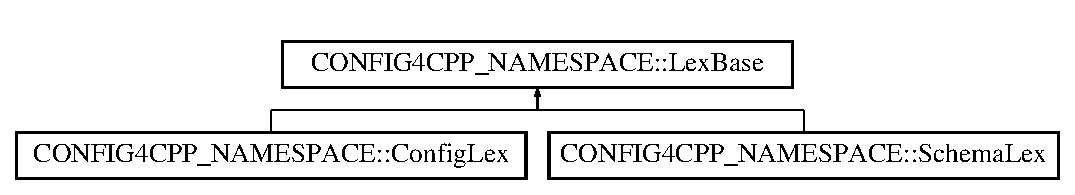
\includegraphics[height=2.000000cm]{classCONFIG4CPP__NAMESPACE_1_1LexBase}
\end{center}
\end{figure}
\subsection*{Classes}
\begin{DoxyCompactItemize}
\item 
struct \hyperlink{structCONFIG4CPP__NAMESPACE_1_1LexBase_1_1FuncInfo}{Func\-Info}
\item 
struct \hyperlink{structCONFIG4CPP__NAMESPACE_1_1LexBase_1_1KeywordInfo}{Keyword\-Info}
\end{DoxyCompactItemize}
\subsection*{Public Types}
\begin{DoxyCompactItemize}
\item 
enum {\bfseries Function\-Type} \{ {\bfseries N\-O\-T\-\_\-\-A\-\_\-\-F\-U\-N\-C} = 1, 
{\bfseries S\-T\-R\-I\-N\-G\-\_\-\-F\-U\-N\-C} = 2, 
{\bfseries L\-I\-S\-T\-\_\-\-F\-U\-N\-C} = 3, 
{\bfseries B\-O\-O\-L\-\_\-\-F\-U\-N\-C} = 4
 \}
\item 
enum {\bfseries Lex\-Base\-Symbols} \{ \\*
{\bfseries L\-E\-X\-\_\-\-I\-D\-E\-N\-T\-\_\-\-S\-Y\-M} = 1, 
{\bfseries L\-E\-X\-\_\-\-S\-E\-M\-I\-C\-O\-L\-O\-N\-\_\-\-S\-Y\-M} = 2, 
{\bfseries L\-E\-X\-\_\-\-P\-L\-U\-S\-\_\-\-S\-Y\-M} = 3, 
{\bfseries L\-E\-X\-\_\-\-Q\-U\-E\-S\-T\-I\-O\-N\-\_\-\-E\-Q\-U\-A\-L\-S\-\_\-\-S\-Y\-M} = 4, 
\\*
{\bfseries L\-E\-X\-\_\-\-E\-Q\-U\-A\-L\-S\-\_\-\-S\-Y\-M} = 5, 
{\bfseries L\-E\-X\-\_\-\-E\-Q\-U\-A\-L\-S\-\_\-\-E\-Q\-U\-A\-L\-S\-\_\-\-S\-Y\-M} = 6, 
{\bfseries L\-E\-X\-\_\-\-N\-O\-T\-\_\-\-E\-Q\-U\-A\-L\-S\-\_\-\-S\-Y\-M} = 7, 
{\bfseries L\-E\-X\-\_\-\-S\-T\-R\-I\-N\-G\-\_\-\-S\-Y\-M} = 8, 
\\*
{\bfseries L\-E\-X\-\_\-\-C\-O\-M\-M\-A\-\_\-\-S\-Y\-M} = 9, 
{\bfseries L\-E\-X\-\_\-\-A\-N\-D\-\_\-\-S\-Y\-M} = 10, 
{\bfseries L\-E\-X\-\_\-\-O\-R\-\_\-\-S\-Y\-M} = 11, 
{\bfseries L\-E\-X\-\_\-\-N\-O\-T\-\_\-\-S\-Y\-M} = 12, 
\\*
{\bfseries L\-E\-X\-\_\-\-A\-T\-\_\-\-S\-Y\-M} = 13, 
{\bfseries L\-E\-X\-\_\-\-O\-P\-E\-N\-\_\-\-B\-R\-A\-C\-K\-E\-T\-\_\-\-S\-Y\-M} = 14, 
{\bfseries L\-E\-X\-\_\-\-C\-L\-O\-S\-E\-\_\-\-B\-R\-A\-C\-K\-E\-T\-\_\-\-S\-Y\-M} = 15, 
{\bfseries L\-E\-X\-\_\-\-O\-P\-E\-N\-\_\-\-B\-R\-A\-C\-E\-\_\-\-S\-Y\-M} = 16, 
\\*
{\bfseries L\-E\-X\-\_\-\-C\-L\-O\-S\-E\-\_\-\-B\-R\-A\-C\-E\-\_\-\-S\-Y\-M} = 17, 
{\bfseries L\-E\-X\-\_\-\-O\-P\-E\-N\-\_\-\-P\-A\-R\-E\-N\-\_\-\-S\-Y\-M} = 18, 
{\bfseries L\-E\-X\-\_\-\-C\-L\-O\-S\-E\-\_\-\-P\-A\-R\-E\-N\-\_\-\-S\-Y\-M} = 19, 
{\bfseries L\-E\-X\-\_\-\-E\-O\-F\-\_\-\-S\-Y\-M} = 20, 
\\*
{\bfseries L\-E\-X\-\_\-\-U\-N\-K\-N\-O\-W\-N\-\_\-\-S\-Y\-M} = 21, 
{\bfseries L\-E\-X\-\_\-\-U\-N\-K\-N\-O\-W\-N\-\_\-\-F\-U\-N\-C\-\_\-\-S\-Y\-M} = 22, 
{\bfseries L\-E\-X\-\_\-\-I\-D\-E\-N\-T\-\_\-\-T\-O\-O\-\_\-\-L\-O\-N\-G\-\_\-\-S\-Y\-M} = 23, 
{\bfseries L\-E\-X\-\_\-\-S\-T\-R\-I\-N\-G\-\_\-\-W\-I\-T\-H\-\_\-\-E\-O\-L\-\_\-\-S\-Y\-M} = 24, 
\\*
{\bfseries L\-E\-X\-\_\-\-I\-L\-L\-E\-G\-A\-L\-\_\-\-I\-D\-E\-N\-T\-\_\-\-S\-Y\-M} = 25, 
{\bfseries L\-E\-X\-\_\-\-T\-W\-O\-\_\-\-D\-O\-T\-S\-\_\-\-I\-D\-E\-N\-T\-\_\-\-S\-Y\-M} = 26, 
{\bfseries L\-E\-X\-\_\-\-B\-L\-O\-C\-K\-\_\-\-S\-T\-R\-I\-N\-G\-\_\-\-W\-I\-T\-H\-\_\-\-E\-O\-F\-\_\-\-S\-Y\-M} = 27, 
{\bfseries L\-E\-X\-\_\-\-S\-O\-L\-E\-\_\-\-D\-O\-T\-\_\-\-I\-D\-E\-N\-T\-\_\-\-S\-Y\-M} = 28
 \}
\end{DoxyCompactItemize}
\subsection*{Public Member Functions}
\begin{DoxyCompactItemize}
\item 
\hypertarget{classCONFIG4CPP__NAMESPACE_1_1LexBase_ac22c286e98a298acb77cf649e9fc7c07}{void {\bfseries next\-Token} (\hyperlink{classCONFIG4CPP__NAMESPACE_1_1LexToken}{Lex\-Token} \&token)}\label{classCONFIG4CPP__NAMESPACE_1_1LexBase_ac22c286e98a298acb77cf649e9fc7c07}

\end{DoxyCompactItemize}
\subsection*{Protected Member Functions}
\begin{DoxyCompactItemize}
\item 
\hypertarget{classCONFIG4CPP__NAMESPACE_1_1LexBase_a6105dd05de2a9c510496b9f42b23e238}{{\bfseries Lex\-Base} (Configuration\-::\-Source\-Type source\-Type, const char $\ast$source, \hyperlink{classCONFIG4CPP__NAMESPACE_1_1UidIdentifierProcessor}{Uid\-Identifier\-Processor} $\ast$uid\-Identifier\-Processor)  throw (\-Configuration\-Exception)}\label{classCONFIG4CPP__NAMESPACE_1_1LexBase_a6105dd05de2a9c510496b9f42b23e238}

\item 
\hypertarget{classCONFIG4CPP__NAMESPACE_1_1LexBase_aea73aeb02d65ce8086297f871d0c6865}{{\bfseries Lex\-Base} (const char $\ast$str)  throw (\-Configuration\-Exception)}\label{classCONFIG4CPP__NAMESPACE_1_1LexBase_aea73aeb02d65ce8086297f871d0c6865}

\end{DoxyCompactItemize}
\subsection*{Protected Attributes}
\begin{DoxyCompactItemize}
\item 
\hypertarget{classCONFIG4CPP__NAMESPACE_1_1LexBase_ae6266e0474783cb87ab2f111431591dd}{\hyperlink{structCONFIG4CPP__NAMESPACE_1_1LexBase_1_1KeywordInfo}{Keyword\-Info} $\ast$ {\bfseries m\-\_\-keyword\-Info\-Array}}\label{classCONFIG4CPP__NAMESPACE_1_1LexBase_ae6266e0474783cb87ab2f111431591dd}

\item 
\hypertarget{classCONFIG4CPP__NAMESPACE_1_1LexBase_a99c1cdbe1124a0c24c972d0c988b674e}{int {\bfseries m\-\_\-keyword\-Info\-Array\-Size}}\label{classCONFIG4CPP__NAMESPACE_1_1LexBase_a99c1cdbe1124a0c24c972d0c988b674e}

\item 
\hypertarget{classCONFIG4CPP__NAMESPACE_1_1LexBase_a4bce40b400287573c3ed00966ee63313}{\hyperlink{structCONFIG4CPP__NAMESPACE_1_1LexBase_1_1FuncInfo}{Func\-Info} $\ast$ {\bfseries m\-\_\-func\-Info\-Array}}\label{classCONFIG4CPP__NAMESPACE_1_1LexBase_a4bce40b400287573c3ed00966ee63313}

\item 
\hypertarget{classCONFIG4CPP__NAMESPACE_1_1LexBase_a167be1b93d17933ddeefa636f8b53af4}{int {\bfseries m\-\_\-func\-Info\-Array\-Size}}\label{classCONFIG4CPP__NAMESPACE_1_1LexBase_a167be1b93d17933ddeefa636f8b53af4}

\end{DoxyCompactItemize}


The documentation for this class was generated from the following files\-:\begin{DoxyCompactItemize}
\item 
src/configuration/config4cpp/src/Lex\-Base.\-h\item 
src/configuration/config4cpp/src/Lex\-Base.\-cpp\end{DoxyCompactItemize}

\hypertarget{classCONFIG4CPP__NAMESPACE_1_1LexToken}{\section{C\-O\-N\-F\-I\-G4\-C\-P\-P\-\_\-\-N\-A\-M\-E\-S\-P\-A\-C\-E\-:\-:Lex\-Token Class Reference}
\label{classCONFIG4CPP__NAMESPACE_1_1LexToken}\index{C\-O\-N\-F\-I\-G4\-C\-P\-P\-\_\-\-N\-A\-M\-E\-S\-P\-A\-C\-E\-::\-Lex\-Token@{C\-O\-N\-F\-I\-G4\-C\-P\-P\-\_\-\-N\-A\-M\-E\-S\-P\-A\-C\-E\-::\-Lex\-Token}}
}
\subsection*{Public Member Functions}
\begin{DoxyCompactItemize}
\item 
\hypertarget{classCONFIG4CPP__NAMESPACE_1_1LexToken_af1d9d8abe647268f458c3e124747e666}{{\bfseries Lex\-Token} (short type, int line\-Num, const char $\ast$spelling)}\label{classCONFIG4CPP__NAMESPACE_1_1LexToken_af1d9d8abe647268f458c3e124747e666}

\item 
\hypertarget{classCONFIG4CPP__NAMESPACE_1_1LexToken_aace473bdcc35b8d51724339db4fa1947}{\hyperlink{classCONFIG4CPP__NAMESPACE_1_1LexToken}{Lex\-Token} \& {\bfseries operator=} (const \hyperlink{classCONFIG4CPP__NAMESPACE_1_1LexToken}{Lex\-Token} \&)}\label{classCONFIG4CPP__NAMESPACE_1_1LexToken_aace473bdcc35b8d51724339db4fa1947}

\item 
\hypertarget{classCONFIG4CPP__NAMESPACE_1_1LexToken_a7764a580ff45dbf380ae257a83fa07c6}{const char $\ast$ {\bfseries spelling} ()}\label{classCONFIG4CPP__NAMESPACE_1_1LexToken_a7764a580ff45dbf380ae257a83fa07c6}

\item 
\hypertarget{classCONFIG4CPP__NAMESPACE_1_1LexToken_a88ee70c3f2fed1da0c33c1f545529f68}{int {\bfseries line\-Num} ()}\label{classCONFIG4CPP__NAMESPACE_1_1LexToken_a88ee70c3f2fed1da0c33c1f545529f68}

\item 
\hypertarget{classCONFIG4CPP__NAMESPACE_1_1LexToken_a227c5c3959085e10b18983b207d87ed4}{short {\bfseries type} ()}\label{classCONFIG4CPP__NAMESPACE_1_1LexToken_a227c5c3959085e10b18983b207d87ed4}

\item 
\hypertarget{classCONFIG4CPP__NAMESPACE_1_1LexToken_a53adb4319a8b16db1fb7c208cfef506a}{const char $\ast$ {\bfseries type\-As\-String} ()}\label{classCONFIG4CPP__NAMESPACE_1_1LexToken_a53adb4319a8b16db1fb7c208cfef506a}

\item 
\hypertarget{classCONFIG4CPP__NAMESPACE_1_1LexToken_ababdad1839b5a4508618272e91c104a2}{bool {\bfseries is\-String\-Func} ()}\label{classCONFIG4CPP__NAMESPACE_1_1LexToken_ababdad1839b5a4508618272e91c104a2}

\item 
\hypertarget{classCONFIG4CPP__NAMESPACE_1_1LexToken_a7fe42e162be433a4d696833d0ac9529d}{bool {\bfseries is\-List\-Func} ()}\label{classCONFIG4CPP__NAMESPACE_1_1LexToken_a7fe42e162be433a4d696833d0ac9529d}

\item 
\hypertarget{classCONFIG4CPP__NAMESPACE_1_1LexToken_a3724c1922d0c063c03fc61363bd59f2a}{bool {\bfseries is\-Bool\-Func} ()}\label{classCONFIG4CPP__NAMESPACE_1_1LexToken_a3724c1922d0c063c03fc61363bd59f2a}

\item 
\hypertarget{classCONFIG4CPP__NAMESPACE_1_1LexToken_a569bf5aea25b35fe55862f8955259177}{void {\bfseries reset} (short type, int line\-Num, const char $\ast$spelling)}\label{classCONFIG4CPP__NAMESPACE_1_1LexToken_a569bf5aea25b35fe55862f8955259177}

\item 
\hypertarget{classCONFIG4CPP__NAMESPACE_1_1LexToken_a6990629405376055c4410c01b91b21dd}{void {\bfseries reset} (short type, int line\-Num, const char $\ast$spelling, short func\-Type)}\label{classCONFIG4CPP__NAMESPACE_1_1LexToken_a6990629405376055c4410c01b91b21dd}

\item 
\hypertarget{classCONFIG4CPP__NAMESPACE_1_1LexToken_a01614ea9e3936c9a2dacc726defaf00e}{void {\bfseries reset\-With\-Ownership} (short type, int line\-Num, \hyperlink{classCONFIG4CPP__NAMESPACE_1_1StringBuffer}{String\-Buffer} \&str)}\label{classCONFIG4CPP__NAMESPACE_1_1LexToken_a01614ea9e3936c9a2dacc726defaf00e}

\end{DoxyCompactItemize}
\subsection*{Protected Attributes}
\begin{DoxyCompactItemize}
\item 
\hypertarget{classCONFIG4CPP__NAMESPACE_1_1LexToken_a59cca9c24306e4e277e8262aa03aff80}{short {\bfseries m\-\_\-type}}\label{classCONFIG4CPP__NAMESPACE_1_1LexToken_a59cca9c24306e4e277e8262aa03aff80}

\item 
\hypertarget{classCONFIG4CPP__NAMESPACE_1_1LexToken_a4eebd8e27e1371036dc2d638f1d929fb}{\hyperlink{classCONFIG4CPP__NAMESPACE_1_1StringBuffer}{String\-Buffer} {\bfseries m\-\_\-spelling}}\label{classCONFIG4CPP__NAMESPACE_1_1LexToken_a4eebd8e27e1371036dc2d638f1d929fb}

\item 
\hypertarget{classCONFIG4CPP__NAMESPACE_1_1LexToken_a8f93bd5b705487011db9cbd3c5e06024}{int {\bfseries m\-\_\-line\-Num}}\label{classCONFIG4CPP__NAMESPACE_1_1LexToken_a8f93bd5b705487011db9cbd3c5e06024}

\item 
\hypertarget{classCONFIG4CPP__NAMESPACE_1_1LexToken_ad01f51ba9f92b166bd96f1c879cdd53c}{short {\bfseries m\-\_\-func\-Type}}\label{classCONFIG4CPP__NAMESPACE_1_1LexToken_ad01f51ba9f92b166bd96f1c879cdd53c}

\end{DoxyCompactItemize}


The documentation for this class was generated from the following files\-:\begin{DoxyCompactItemize}
\item 
src/configuration/config4cpp/src/Lex\-Token.\-h\item 
src/configuration/config4cpp/src/Lex\-Token.\-cpp\end{DoxyCompactItemize}

\hypertarget{classLFOWorkshopSPU}{}\section{L\+F\+O\+Workshop\+S\+PU Class Reference}
\label{classLFOWorkshopSPU}\index{L\+F\+O\+Workshop\+S\+PU@{L\+F\+O\+Workshop\+S\+PU}}
Inheritance diagram for L\+F\+O\+Workshop\+S\+PU\+:\begin{figure}[H]
\begin{center}
\leavevmode
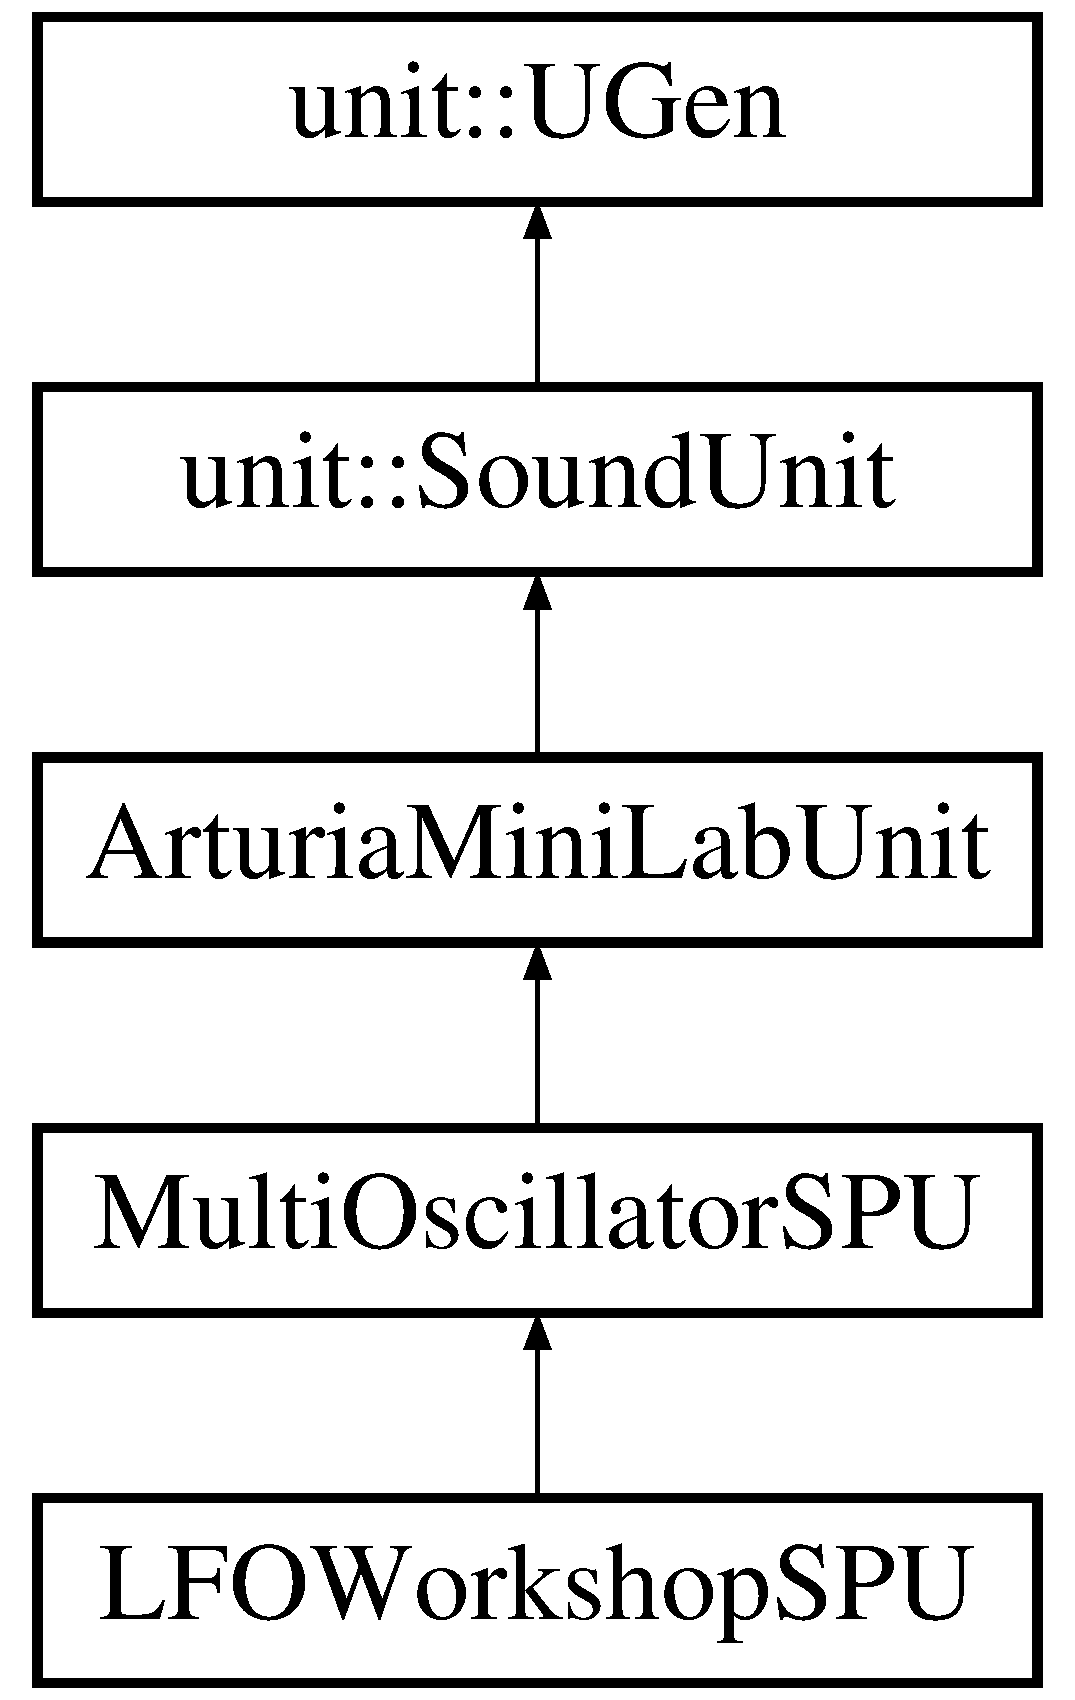
\includegraphics[height=5.000000cm]{classLFOWorkshopSPU}
\end{center}
\end{figure}
\subsection*{Public Member Functions}
\begin{DoxyCompactItemize}
\item 
{\bfseries L\+F\+O\+Workshop\+S\+PU} (std\+::string name)\hypertarget{classLFOWorkshopSPU_af0da7426287c75e69999066976565005}{}\label{classLFOWorkshopSPU_af0da7426287c75e69999066976565005}

\item 
float {\bfseries tick} ()\hypertarget{classLFOWorkshopSPU_a0af8aaed492cecf1b6d3bf416393a8d1}{}\label{classLFOWorkshopSPU_a0af8aaed492cecf1b6d3bf416393a8d1}

\item 
void {\bfseries control} (std\+::string port\+Name, float value)\hypertarget{classLFOWorkshopSPU_a3c139a87ec2ec0c9cfa149f7652b11f8}{}\label{classLFOWorkshopSPU_a3c139a87ec2ec0c9cfa149f7652b11f8}

\end{DoxyCompactItemize}
\subsection*{Additional Inherited Members}


The documentation for this class was generated from the following files\+:\begin{DoxyCompactItemize}
\item 
include/L\+F\+O\+Workshop\+S\+P\+U.\+h\item 
spu/L\+F\+O\+Workshop\+S\+P\+U.\+cpp\end{DoxyCompactItemize}

\hypertarget{classCONFIG4CPP__NAMESPACE_1_1MBChar}{\section{C\-O\-N\-F\-I\-G4\-C\-P\-P\-\_\-\-N\-A\-M\-E\-S\-P\-A\-C\-E\-:\-:M\-B\-Char Class Reference}
\label{classCONFIG4CPP__NAMESPACE_1_1MBChar}\index{C\-O\-N\-F\-I\-G4\-C\-P\-P\-\_\-\-N\-A\-M\-E\-S\-P\-A\-C\-E\-::\-M\-B\-Char@{C\-O\-N\-F\-I\-G4\-C\-P\-P\-\_\-\-N\-A\-M\-E\-S\-P\-A\-C\-E\-::\-M\-B\-Char}}
}
\subsection*{Public Member Functions}
\begin{DoxyCompactItemize}
\item 
\hypertarget{classCONFIG4CPP__NAMESPACE_1_1MBChar_a8148d061decb5da0d1ab30c4ff309026}{bool {\bfseries add} (char ch)}\label{classCONFIG4CPP__NAMESPACE_1_1MBChar_a8148d061decb5da0d1ab30c4ff309026}

\item 
\hypertarget{classCONFIG4CPP__NAMESPACE_1_1MBChar_a1003f4b0c976c28244cff7f9d222fb74}{const char $\ast$ {\bfseries c\-\_\-str} () const }\label{classCONFIG4CPP__NAMESPACE_1_1MBChar_a1003f4b0c976c28244cff7f9d222fb74}

\item 
\hypertarget{classCONFIG4CPP__NAMESPACE_1_1MBChar_a2658f6778bcd1d6f3c00b07426bfaea3}{int {\bfseries length} () const }\label{classCONFIG4CPP__NAMESPACE_1_1MBChar_a2658f6778bcd1d6f3c00b07426bfaea3}

\item 
\hypertarget{classCONFIG4CPP__NAMESPACE_1_1MBChar_a6ee4ba3a206e9cd7bc438b61fbee9b73}{void {\bfseries set\-W\-Char} (wchar\-\_\-t w\-Char)}\label{classCONFIG4CPP__NAMESPACE_1_1MBChar_a6ee4ba3a206e9cd7bc438b61fbee9b73}

\item 
\hypertarget{classCONFIG4CPP__NAMESPACE_1_1MBChar_ac4b8e859135f90a9b2943b189b610291}{wchar\-\_\-t {\bfseries get\-W\-Char} () const }\label{classCONFIG4CPP__NAMESPACE_1_1MBChar_ac4b8e859135f90a9b2943b189b610291}

\item 
\hypertarget{classCONFIG4CPP__NAMESPACE_1_1MBChar_aeb8283f31625266ca7024de92165d3a1}{bool {\bfseries is\-Space} () const }\label{classCONFIG4CPP__NAMESPACE_1_1MBChar_aeb8283f31625266ca7024de92165d3a1}

\item 
\hypertarget{classCONFIG4CPP__NAMESPACE_1_1MBChar_a444a68c1b4e0b193e0504b4bd1df62c6}{bool {\bfseries is\-Empty} () const }\label{classCONFIG4CPP__NAMESPACE_1_1MBChar_a444a68c1b4e0b193e0504b4bd1df62c6}

\item 
\hypertarget{classCONFIG4CPP__NAMESPACE_1_1MBChar_a9baa83966e8acd7d1450524896a49482}{bool {\bfseries is\-Full} () const }\label{classCONFIG4CPP__NAMESPACE_1_1MBChar_a9baa83966e8acd7d1450524896a49482}

\item 
\hypertarget{classCONFIG4CPP__NAMESPACE_1_1MBChar_aa860c417472454ddee7188d1ccc0953a}{void {\bfseries reset} ()}\label{classCONFIG4CPP__NAMESPACE_1_1MBChar_aa860c417472454ddee7188d1ccc0953a}

\item 
\hypertarget{classCONFIG4CPP__NAMESPACE_1_1MBChar_a878a74cc2166862225f75b845f5b413f}{\hyperlink{classCONFIG4CPP__NAMESPACE_1_1MBChar}{M\-B\-Char} \& {\bfseries operator=} (const \hyperlink{classCONFIG4CPP__NAMESPACE_1_1MBChar}{M\-B\-Char} \&)}\label{classCONFIG4CPP__NAMESPACE_1_1MBChar_a878a74cc2166862225f75b845f5b413f}

\item 
\hypertarget{classCONFIG4CPP__NAMESPACE_1_1MBChar_ad766099ec2d566e8b7d954f661c88ac6}{\hyperlink{classCONFIG4CPP__NAMESPACE_1_1MBChar}{M\-B\-Char} \& {\bfseries operator=} (char ch)}\label{classCONFIG4CPP__NAMESPACE_1_1MBChar_ad766099ec2d566e8b7d954f661c88ac6}

\item 
\hypertarget{classCONFIG4CPP__NAMESPACE_1_1MBChar_abaa807b2ac2d3c831636e6ac42619518}{bool {\bfseries operator==} (const \hyperlink{classCONFIG4CPP__NAMESPACE_1_1MBChar}{M\-B\-Char} \&other) const }\label{classCONFIG4CPP__NAMESPACE_1_1MBChar_abaa807b2ac2d3c831636e6ac42619518}

\item 
\hypertarget{classCONFIG4CPP__NAMESPACE_1_1MBChar_a9a6674574e2e0b6db79bf47314e4d3e9}{bool {\bfseries operator!=} (const \hyperlink{classCONFIG4CPP__NAMESPACE_1_1MBChar}{M\-B\-Char} \&other) const }\label{classCONFIG4CPP__NAMESPACE_1_1MBChar_a9a6674574e2e0b6db79bf47314e4d3e9}

\item 
\hypertarget{classCONFIG4CPP__NAMESPACE_1_1MBChar_afa4f42bacc6b83819b3ee542c0378791}{bool {\bfseries operator==} (char ch) const }\label{classCONFIG4CPP__NAMESPACE_1_1MBChar_afa4f42bacc6b83819b3ee542c0378791}

\item 
\hypertarget{classCONFIG4CPP__NAMESPACE_1_1MBChar_a7168a9754d0bfb7dd5cdde9f90901d4e}{bool {\bfseries operator!=} (char ch) const }\label{classCONFIG4CPP__NAMESPACE_1_1MBChar_a7168a9754d0bfb7dd5cdde9f90901d4e}

\end{DoxyCompactItemize}


The documentation for this class was generated from the following files\-:\begin{DoxyCompactItemize}
\item 
src/configuration/config4cpp/src/M\-B\-Char.\-h\item 
src/configuration/config4cpp/src/M\-B\-Char.\-cpp\end{DoxyCompactItemize}

\hypertarget{classosc_1_1MessageData}{\section{osc\-:\-:Message\-Data Class Reference}
\label{classosc_1_1MessageData}\index{osc\-::\-Message\-Data@{osc\-::\-Message\-Data}}
}


{\ttfamily \#include $<$Message\-Data.\-h$>$}

\subsection*{Public Types}
\begin{DoxyCompactItemize}
\item 
enum {\bfseries Types} \{ \\*
{\bfseries M\-I\-D\-I\-O\-N}, 
{\bfseries M\-I\-D\-I\-O\-F\-F}, 
{\bfseries C\-O\-N\-T\-R\-O\-L}, 
{\bfseries P\-A\-D\-O\-N}, 
\\*
{\bfseries P\-A\-D\-O\-F\-F}, 
{\bfseries S\-L\-I\-D\-E\-R}, 
{\bfseries U\-N\-K\-N\-O\-W\-N}
 \}
\end{DoxyCompactItemize}
\subsection*{Public Member Functions}
\begin{DoxyCompactItemize}
\item 
\hypertarget{classosc_1_1MessageData_af370333b9828ad63ba1031ac941300c2}{{\bfseries Message\-Data} (std\-::string s, int a1, int a2, int a3, float f)}\label{classosc_1_1MessageData_af370333b9828ad63ba1031ac941300c2}

\item 
\hypertarget{classosc_1_1MessageData_acf5694351e2f877340d6b38044d8b2d3}{{\bfseries Message\-Data} (\hyperlink{classosc_1_1MessageData}{Message\-Data} $\ast$md)}\label{classosc_1_1MessageData_acf5694351e2f877340d6b38044d8b2d3}

\item 
\hypertarget{classosc_1_1MessageData_a8bf658a5be5789142fa260512fded9a1}{std\-::string {\bfseries get\-Message} ()}\label{classosc_1_1MessageData_a8bf658a5be5789142fa260512fded9a1}

\item 
\hypertarget{classosc_1_1MessageData_aa625a45bf78b8351d29a7696c8f014e9}{int {\bfseries get\-Code} ()}\label{classosc_1_1MessageData_aa625a45bf78b8351d29a7696c8f014e9}

\item 
\hypertarget{classosc_1_1MessageData_ab70773361a5ffba488a83b0d87cfb25c}{int {\bfseries get\-Key} ()}\label{classosc_1_1MessageData_ab70773361a5ffba488a83b0d87cfb25c}

\item 
\hypertarget{classosc_1_1MessageData_af79bf248fbb542bd25984f7f2b3993eb}{int {\bfseries get\-Value} ()}\label{classosc_1_1MessageData_af79bf248fbb542bd25984f7f2b3993eb}

\item 
\hypertarget{classosc_1_1MessageData_ad1e951e980e59c5d222b79856cae6d32}{float {\bfseries get\-F1} ()}\label{classosc_1_1MessageData_ad1e951e980e59c5d222b79856cae6d32}

\item 
\hypertarget{classosc_1_1MessageData_a38c69b7ebcf46e7c19ff2409af36a7ae}{Types {\bfseries get\-Type} ()}\label{classosc_1_1MessageData_a38c69b7ebcf46e7c19ff2409af36a7ae}

\item 
\hypertarget{classosc_1_1MessageData_a1da8f45a1453c7d11029fa360d7a642c}{void {\bfseries set\-Message} (std\-::string s)}\label{classosc_1_1MessageData_a1da8f45a1453c7d11029fa360d7a642c}

\item 
\hypertarget{classosc_1_1MessageData_a0f8ce5f6d5c4452e26656236ee7aefc3}{void {\bfseries adapt\-Message\-Type} ()}\label{classosc_1_1MessageData_a0f8ce5f6d5c4452e26656236ee7aefc3}

\item 
\hypertarget{classosc_1_1MessageData_a8639583a844208ccae9568bb68d1e547}{void {\bfseries set\-Code} (int a1)}\label{classosc_1_1MessageData_a8639583a844208ccae9568bb68d1e547}

\item 
\hypertarget{classosc_1_1MessageData_a54a0ddfb44fba671ba243914b037e231}{void {\bfseries set\-Key} (int a2)}\label{classosc_1_1MessageData_a54a0ddfb44fba671ba243914b037e231}

\item 
\hypertarget{classosc_1_1MessageData_a24e273f0a4443505ccf6222405cfb567}{void {\bfseries set\-Value} (int a3)}\label{classosc_1_1MessageData_a24e273f0a4443505ccf6222405cfb567}

\item 
\hypertarget{classosc_1_1MessageData_a94dce06ace95a93c075dbaf253e559fe}{void {\bfseries set\-F1} (float f)}\label{classosc_1_1MessageData_a94dce06ace95a93c075dbaf253e559fe}

\item 
\hypertarget{classosc_1_1MessageData_a9eb7741e4216075b0e03c554d83e35ae}{void {\bfseries set\-Message\-Data} (std\-::string s, int a1, int a2, int a3, float f)}\label{classosc_1_1MessageData_a9eb7741e4216075b0e03c554d83e35ae}

\item 
\hypertarget{classosc_1_1MessageData_a169f4e7ec5a0eb896cfccd8186b5fe8d}{bool {\bfseries is\-Fresh} ()}\label{classosc_1_1MessageData_a169f4e7ec5a0eb896cfccd8186b5fe8d}

\end{DoxyCompactItemize}


\subsection{Detailed Description}
\hyperlink{classosc_1_1MessageData}{Message\-Data} encapsulates the data of a osc midi message. It stores the message, key, value (velocity), an optional float, and the message type.

\begin{DoxyAuthor}{Author}
jtm, email\-:  \href{mailto:milde@hs-fulda.de}{\tt milde@hs-\/fulda.\-de} 
\end{DoxyAuthor}
\begin{DoxySince}{Since}
04-\/2016 
\end{DoxySince}
\begin{DoxyVersion}{Version}
1.\-0 
\end{DoxyVersion}


The documentation for this class was generated from the following files\-:\begin{DoxyCompactItemize}
\item 
include/Message\-Data.\-h\item 
osc/Message\-Data.\-cpp\end{DoxyCompactItemize}

\hypertarget{classMessageDataQueue}{}\section{Message\+Data\+Queue Class Reference}
\label{classMessageDataQueue}\index{Message\+Data\+Queue@{Message\+Data\+Queue}}
\subsection*{Public Member Functions}
\begin{DoxyCompactItemize}
\item 
void {\bfseries add} (\hyperlink{classMessageData}{Message\+Data} $\ast$m)\hypertarget{classMessageDataQueue_aa31f6a8bed7000525d09716de264a049}{}\label{classMessageDataQueue_aa31f6a8bed7000525d09716de264a049}

\item 
\hyperlink{classMessageData}{Message\+Data} $\ast$ {\bfseries get} ()\hypertarget{classMessageDataQueue_ace0bab37a7339c7a0eb813f80a03c88d}{}\label{classMessageDataQueue_ace0bab37a7339c7a0eb813f80a03c88d}

\item 
int {\bfseries size} ()\hypertarget{classMessageDataQueue_a6f7619c03371e76b95a2c2d348da866d}{}\label{classMessageDataQueue_a6f7619c03371e76b95a2c2d348da866d}

\item 
void {\bfseries clear} ()\hypertarget{classMessageDataQueue_a565232895a0e0cc0416715aedf2e5e21}{}\label{classMessageDataQueue_a565232895a0e0cc0416715aedf2e5e21}

\end{DoxyCompactItemize}


The documentation for this class was generated from the following files\+:\begin{DoxyCompactItemize}
\item 
store/Message\+Data\+Queue.\+h\item 
store/Message\+Data\+Queue.\+cpp\end{DoxyCompactItemize}

\hypertarget{classosc_1_1MidiConnector}{}\section{osc\+:\+:Midi\+Connector Class Reference}
\label{classosc_1_1MidiConnector}\index{osc\+::\+Midi\+Connector@{osc\+::\+Midi\+Connector}}
\subsection*{Public Member Functions}
\begin{DoxyCompactItemize}
\item 
{\bfseries Midi\+Connector} (int p)\hypertarget{classosc_1_1MidiConnector_a1629e8c842409a21dbc78258794556cc}{}\label{classosc_1_1MidiConnector_a1629e8c842409a21dbc78258794556cc}

\item 
void {\bfseries send\+Message} (std\+::string message\+Type, int code, int key, int value, float f1)\hypertarget{classosc_1_1MidiConnector_a700ee4383b29cd2bdc73f7cfc61a360e}{}\label{classosc_1_1MidiConnector_a700ee4383b29cd2bdc73f7cfc61a360e}

\end{DoxyCompactItemize}


The documentation for this class was generated from the following files\+:\begin{DoxyCompactItemize}
\item 
osc/Midi\+Connector.\+h\item 
osc/Midi\+Connector.\+cpp\end{DoxyCompactItemize}

\hypertarget{classunit_1_1MidiInputGen}{\section{unit\-:\-:Midi\-Input\-Gen Class Reference}
\label{classunit_1_1MidiInputGen}\index{unit\-::\-Midi\-Input\-Gen@{unit\-::\-Midi\-Input\-Gen}}
}


{\ttfamily \#include $<$Midi\-Input\-Gen.\-h$>$}

Inheritance diagram for unit\-:\-:Midi\-Input\-Gen\-:\begin{figure}[H]
\begin{center}
\leavevmode
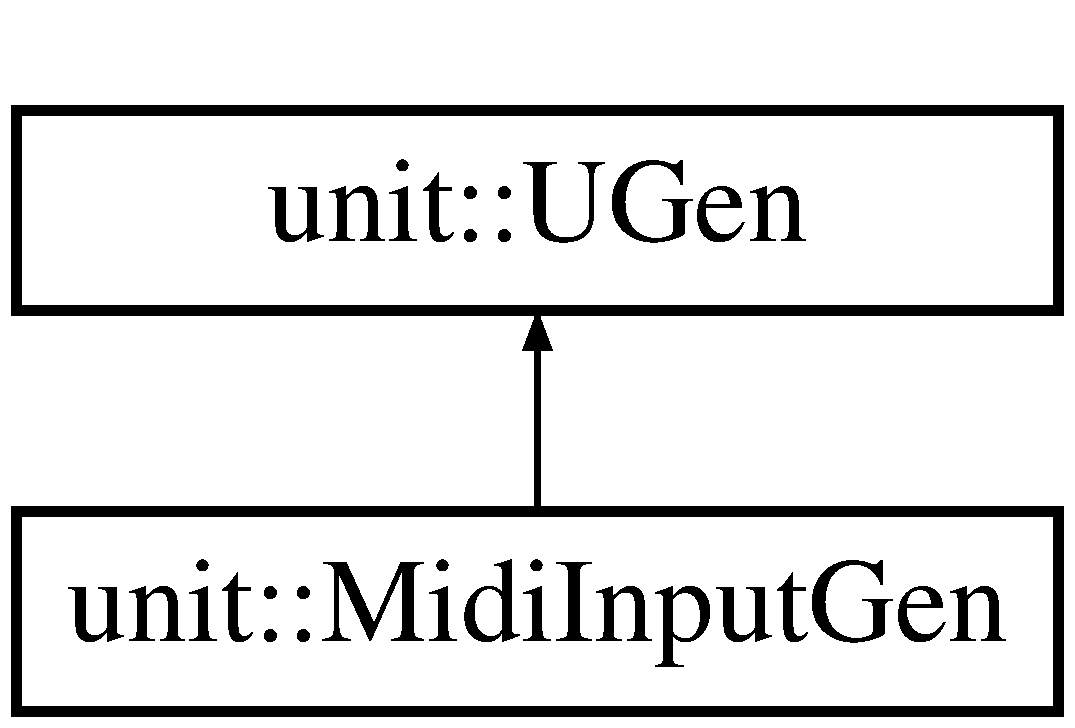
\includegraphics[height=2.000000cm]{classunit_1_1MidiInputGen}
\end{center}
\end{figure}
\subsection*{Public Member Functions}
\begin{DoxyCompactItemize}
\item 
\hypertarget{classunit_1_1MidiInputGen_a48063ea203958867e649466152ccebd8}{{\bfseries Midi\-Input\-Gen} (std\-::string name)}\label{classunit_1_1MidiInputGen_a48063ea203958867e649466152ccebd8}

\item 
\hypertarget{classunit_1_1MidiInputGen_a4633d43acd7810f80ebc3ac343ba7dd3}{float {\bfseries tick} ()}\label{classunit_1_1MidiInputGen_a4633d43acd7810f80ebc3ac343ba7dd3}

\item 
\hypertarget{classunit_1_1MidiInputGen_a97db1d2b3deac8d7dd09fce65bfdca04}{void {\bfseries control} (std\-::string port\-Name, float value)}\label{classunit_1_1MidiInputGen_a97db1d2b3deac8d7dd09fce65bfdca04}

\item 
\hypertarget{classunit_1_1MidiInputGen_aa180744b692b2ac4f8f5d11ef2adc245}{float {\bfseries get\-Key} ()}\label{classunit_1_1MidiInputGen_aa180744b692b2ac4f8f5d11ef2adc245}

\item 
\hypertarget{classunit_1_1MidiInputGen_a4e39971e955b7052df07dd9413075fc0}{float {\bfseries get\-Velocity} ()}\label{classunit_1_1MidiInputGen_a4e39971e955b7052df07dd9413075fc0}

\item 
\hypertarget{classunit_1_1MidiInputGen_a9bfcd695b0dd9a3c3b0ca8cddadd9432}{float {\bfseries get\-Gate} ()}\label{classunit_1_1MidiInputGen_a9bfcd695b0dd9a3c3b0ca8cddadd9432}

\item 
\hypertarget{classunit_1_1MidiInputGen_a4db32a60d580040a10d3b0acad2c30e3}{float {\bfseries get\-Trigger} ()}\label{classunit_1_1MidiInputGen_a4db32a60d580040a10d3b0acad2c30e3}

\end{DoxyCompactItemize}
\subsection*{Additional Inherited Members}


\subsection{Detailed Description}
\hyperlink{classunit_1_1MidiInputGen}{Midi\-Input\-Gen} processes the incoming midi messages and generates the gate and the trigger signals.

Use a \hyperlink{classunit_1_1MidiInputGen}{Midi\-Input\-Gen} as the first \hyperlink{classunit_1_1UGen}{U\-Gen} in a \hyperlink{classunit_1_1SoundUnit}{Sound\-Unit} in order to get the current status of midi input. More specifically\-: use the gate and trigger value to control the sound synthesis.


\begin{DoxyItemize}
\item {\bfseries tick()} is providing the current {\bfseries gate} value.
\item the trigger is kept up (1.\-0) for exactly one tick() call.
\item the gate is kept up (1.\-0) for as long as there are more {\bfseries midi on} than {\bfseries midi off} events
\item the {\bfseries gate} is stored in {\bfseries out1}.
\item the {\bfseries trigger} is stored in {\bfseries out2}.
\end{DoxyItemize}

Control-\/\-Interface


\begin{DoxyItemize}
\item control(\char`\"{}midi on\char`\"{}, value) processes {\bfseries midi on} event. {\bfseries value} should hold the key.
\item control(\char`\"{}midi off\char`\"{}, value) processes {\bfseries midi off} event. {\bfseries value} should hold the key.
\item control(\char`\"{}velocity\char`\"{}, value) sets the {\bfseries velocity} of the current key.
\item control(\char`\"{}reset\char`\"{}, value) resets the counts, trigger is 0, gate is 0.
\end{DoxyItemize}

Fast access functions


\begin{DoxyItemize}
\item {\bfseries get\-Key()}\-: returns the current key.
\item {\bfseries get\-Velocity()}\-: returns the current velocity.
\item {\bfseries get\-Trigger()}\-: returns the current trigger value.
\item {\bfseries get\-Gate()}\-: returns the current gate value.
\end{DoxyItemize}

\begin{DoxyAuthor}{Author}
jtm, email\-:  \href{mailto:milde@hs-fulda.de}{\tt milde@hs-\/fulda.\-de} 
\end{DoxyAuthor}
\begin{DoxySince}{Since}
04-\/2016 
\end{DoxySince}
\begin{DoxyVersion}{Version}
1.\-0 
\end{DoxyVersion}


The documentation for this class was generated from the following files\-:\begin{DoxyCompactItemize}
\item 
include/Midi\-Input\-Gen.\-h\item 
unit/Midi\-Input\-Gen.\-cpp\end{DoxyCompactItemize}

\hypertarget{classOscInConnector_1_1MidiPacketListener}{}\section{Osc\+In\+Connector\+:\+:Midi\+Packet\+Listener Class Reference}
\label{classOscInConnector_1_1MidiPacketListener}\index{Osc\+In\+Connector\+::\+Midi\+Packet\+Listener@{Osc\+In\+Connector\+::\+Midi\+Packet\+Listener}}
Inheritance diagram for Osc\+In\+Connector\+:\+:Midi\+Packet\+Listener\+:\begin{figure}[H]
\begin{center}
\leavevmode
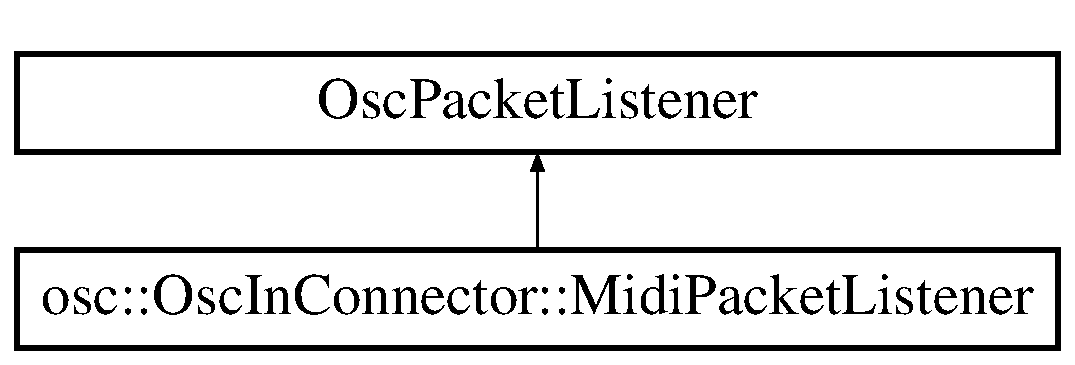
\includegraphics[height=2.000000cm]{classOscInConnector_1_1MidiPacketListener}
\end{center}
\end{figure}
\subsection*{Public Member Functions}
\begin{DoxyCompactItemize}
\item 
void {\bfseries set\+Osc\+In} (\hyperlink{classOscInConnector}{Osc\+In\+Connector} $\ast$o)\hypertarget{classOscInConnector_1_1MidiPacketListener_ab4e0346cad409b3871add20bc5c8c904}{}\label{classOscInConnector_1_1MidiPacketListener_ab4e0346cad409b3871add20bc5c8c904}

\item 
int {\bfseries get\+Port} ()\hypertarget{classOscInConnector_1_1MidiPacketListener_affd65358cd1ffcde113576b8023fa8d6}{}\label{classOscInConnector_1_1MidiPacketListener_affd65358cd1ffcde113576b8023fa8d6}

\end{DoxyCompactItemize}
\subsection*{Protected Member Functions}
\begin{DoxyCompactItemize}
\item 
void {\bfseries write\+Data} (std\+::string s, int a1, int a2, int a3, float f)\hypertarget{classOscInConnector_1_1MidiPacketListener_a6ad19bb71d7d360d432eecd4d2f8aa0f}{}\label{classOscInConnector_1_1MidiPacketListener_a6ad19bb71d7d360d432eecd4d2f8aa0f}

\item 
virtual void {\bfseries Process\+Message} (const osc\+::\+Received\+Message \&m, const Ip\+Endpoint\+Name \&remote\+Endpoint)\hypertarget{classOscInConnector_1_1MidiPacketListener_ad5b4e469c87859e8577d2bf77aaa66bd}{}\label{classOscInConnector_1_1MidiPacketListener_ad5b4e469c87859e8577d2bf77aaa66bd}

\end{DoxyCompactItemize}


The documentation for this class was generated from the following file\+:\begin{DoxyCompactItemize}
\item 
Osc\+In\+Connector.\+cpp\end{DoxyCompactItemize}

\hypertarget{classutil_1_1MidiUtil}{\section{util\-:\-:Midi\-Util Class Reference}
\label{classutil_1_1MidiUtil}\index{util\-::\-Midi\-Util@{util\-::\-Midi\-Util}}
}
\subsection*{Static Public Member Functions}
\begin{DoxyCompactItemize}
\item 
\hypertarget{classutil_1_1MidiUtil_a04b46794718bd5d4eeaa58b110bea689}{static float {\bfseries midi2frequency} (int key)}\label{classutil_1_1MidiUtil_a04b46794718bd5d4eeaa58b110bea689}

\end{DoxyCompactItemize}


The documentation for this class was generated from the following files\-:\begin{DoxyCompactItemize}
\item 
include/Midi\-Util.\-h\item 
util/Midi\-Util.\-cpp\end{DoxyCompactItemize}

\hypertarget{classunit_1_1MoogVCFGen}{\section{unit\-:\-:Moog\-V\-C\-F\-Gen Class Reference}
\label{classunit_1_1MoogVCFGen}\index{unit\-::\-Moog\-V\-C\-F\-Gen@{unit\-::\-Moog\-V\-C\-F\-Gen}}
}


{\ttfamily \#include $<$Moog\-V\-C\-F\-Gen.\-h$>$}

Inheritance diagram for unit\-:\-:Moog\-V\-C\-F\-Gen\-:\begin{figure}[H]
\begin{center}
\leavevmode
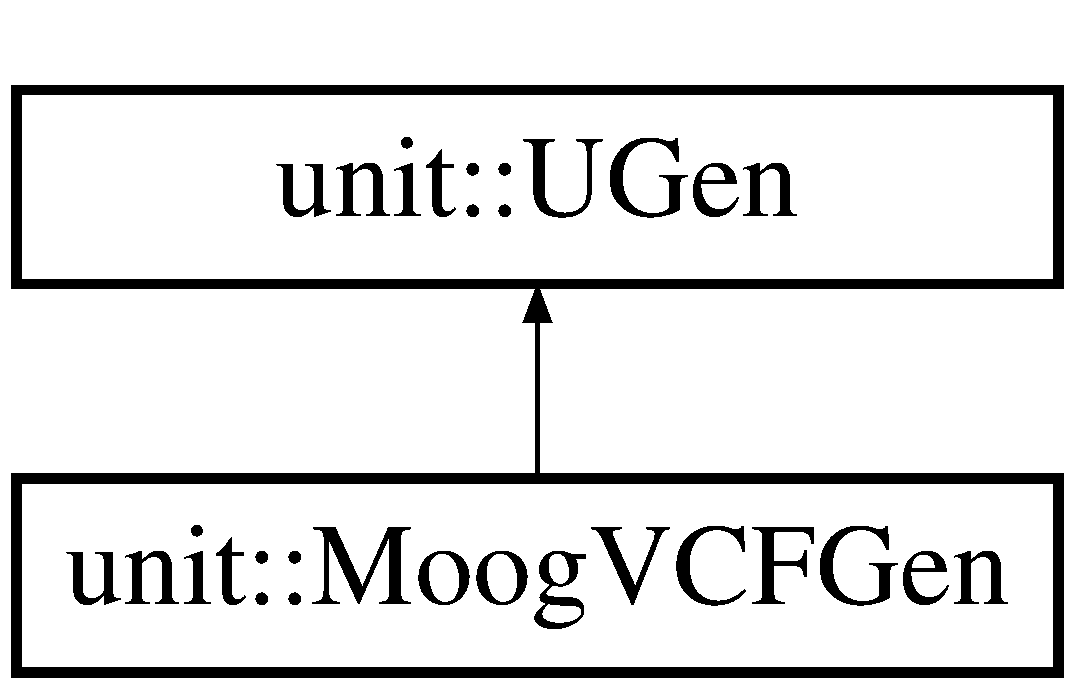
\includegraphics[height=2.000000cm]{classunit_1_1MoogVCFGen}
\end{center}
\end{figure}
\subsection*{Public Member Functions}
\begin{DoxyCompactItemize}
\item 
\hypertarget{classunit_1_1MoogVCFGen_a7c93093d236bb363567929178f40a7a0}{{\bfseries Moog\-V\-C\-F\-Gen} (std\-::string name)}\label{classunit_1_1MoogVCFGen_a7c93093d236bb363567929178f40a7a0}

\item 
\hypertarget{classunit_1_1MoogVCFGen_a949c02a370ff5ce83b6dcf9a87eafba0}{float {\bfseries tick} ()}\label{classunit_1_1MoogVCFGen_a949c02a370ff5ce83b6dcf9a87eafba0}

\item 
\hypertarget{classunit_1_1MoogVCFGen_acedc61969800d26d1d5345fd23ea22c7}{void {\bfseries control} (std\-::string port\-Name, float value)}\label{classunit_1_1MoogVCFGen_acedc61969800d26d1d5345fd23ea22c7}

\item 
\hypertarget{classunit_1_1MoogVCFGen_a047c043cf3fcf1ac972bc088fa86f6f3}{void {\bfseries set\-Cutoff} (float v)}\label{classunit_1_1MoogVCFGen_a047c043cf3fcf1ac972bc088fa86f6f3}

\item 
\hypertarget{classunit_1_1MoogVCFGen_a9a0c38cd5912e817e89bed1b69eb0e39}{void {\bfseries set\-Resonance} (float v)}\label{classunit_1_1MoogVCFGen_a9a0c38cd5912e817e89bed1b69eb0e39}

\end{DoxyCompactItemize}
\subsection*{Additional Inherited Members}


\subsection{Detailed Description}
\hyperlink{classunit_1_1MoogVCFGen}{Moog\-V\-C\-F\-Gen} is approximating the 4 ladder Moog lowpass. Type \-: 24db resonant lowpass References \-: C\-Sound source code, Stilson/\-Smith C\-C\-R\-M\-A paper.

Filtering the in port {\bfseries in1}, {\bfseries out1} stores the output value.


\begin{DoxyItemize}
\item {\bfseries tick()} is providing the filtered input value.
\end{DoxyItemize}

Control-\/\-Interface


\begin{DoxyItemize}
\item {\bfseries control(\char`\"{}cutoff\char`\"{}, value)}\-: \mbox{[}0-\/1\mbox{]} is mapped to \mbox{[}20-\/22050\mbox{]}
\item {\bfseries control(\char`\"{}resonance\char`\"{}, value)}\-: \mbox{[}0-\/1\mbox{]} is mapped to \mbox{[}0-\/1\mbox{]}
\end{DoxyItemize}

Fast access functions
\begin{DoxyItemize}
\item set\-Cutoff(float v);
\item set\-Resonance(float v);
\item the standard fast access functions
\end{DoxyItemize}

\begin{DoxyAuthor}{Author}
jtm, email\-:  \href{mailto:milde@hs-fulda.de}{\tt milde@hs-\/fulda.\-de} 
\end{DoxyAuthor}
\begin{DoxySince}{Since}
04-\/2016 
\end{DoxySince}
\begin{DoxyVersion}{Version}
1.\-0 
\end{DoxyVersion}


The documentation for this class was generated from the following files\-:\begin{DoxyCompactItemize}
\item 
src/include/Moog\-V\-C\-F\-Gen.\-h\item 
src/unit/Moog\-V\-C\-F\-Gen.\-cpp\end{DoxyCompactItemize}

\hypertarget{classMultiOscillatorSPU}{}\section{Multi\+Oscillator\+S\+PU Class Reference}
\label{classMultiOscillatorSPU}\index{Multi\+Oscillator\+S\+PU@{Multi\+Oscillator\+S\+PU}}


{\ttfamily \#include $<$Multi\+Oscillator\+S\+P\+U.\+h$>$}

Inheritance diagram for Multi\+Oscillator\+S\+PU\+:\begin{figure}[H]
\begin{center}
\leavevmode
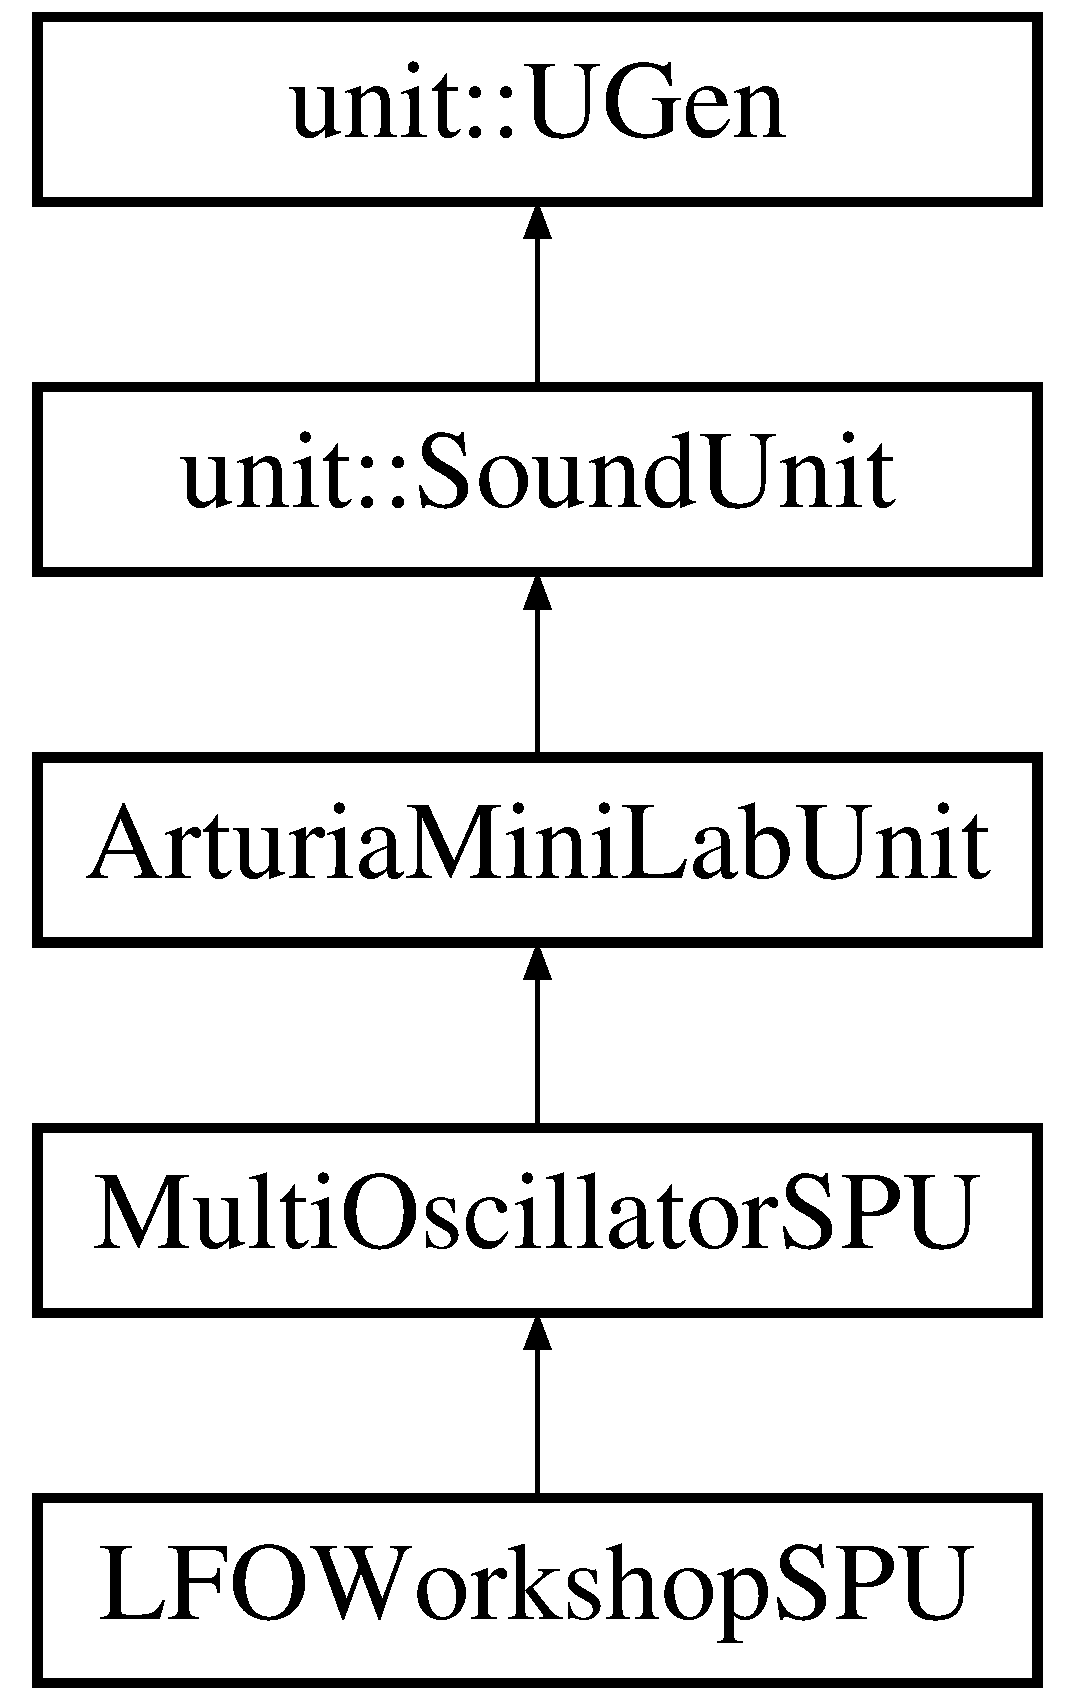
\includegraphics[height=5.000000cm]{classMultiOscillatorSPU}
\end{center}
\end{figure}
\subsection*{Public Member Functions}
\begin{DoxyCompactItemize}
\item 
{\bfseries Multi\+Oscillator\+S\+PU} (std\+::string name)\hypertarget{classMultiOscillatorSPU_a3c7fc8e1067fb1b025551702344597a6}{}\label{classMultiOscillatorSPU_a3c7fc8e1067fb1b025551702344597a6}

\item 
float {\bfseries tick} ()\hypertarget{classMultiOscillatorSPU_ac5004f7b5bfa6025abee24b53abdd69f}{}\label{classMultiOscillatorSPU_ac5004f7b5bfa6025abee24b53abdd69f}

\item 
void {\bfseries control} (std\+::string port\+Name, float value)\hypertarget{classMultiOscillatorSPU_ab20794e0a79b779f35b36582cf4f65d0}{}\label{classMultiOscillatorSPU_ab20794e0a79b779f35b36582cf4f65d0}

\item 
void {\bfseries set\+Frequency\+Mod} (float value)\hypertarget{classMultiOscillatorSPU_a7040cf4388fe9bdaf624b707973241d0}{}\label{classMultiOscillatorSPU_a7040cf4388fe9bdaf624b707973241d0}

\item 
void {\bfseries set\+Pulse\+Width\+Mod} (float value)\hypertarget{classMultiOscillatorSPU_a42f7950c4fac230d97f43fa22587064e}{}\label{classMultiOscillatorSPU_a42f7950c4fac230d97f43fa22587064e}

\end{DoxyCompactItemize}
\subsection*{Additional Inherited Members}


\subsection{Detailed Description}
\hyperlink{classMultiOscillatorSPU}{Multi\+Oscillator\+S\+PU} provides a selectable multi oscillator providing all of the available oscillators.

Currently (9.\+5.\+2016) these are\+: Pulse\+Gen, Saw\+Gen, Cosine\+Gen, Square\+Gen, and Noise\+Gen.

\begin{DoxyAuthor}{Author}
jtm, email\+:  \href{mailto:milde@hs-fulda.de}{\tt milde@hs-\/fulda.\+de} 
\end{DoxyAuthor}
\begin{DoxySince}{Since}
04-\/2016 
\end{DoxySince}
\begin{DoxyVersion}{Version}
1.\+0 
\end{DoxyVersion}


The documentation for this class was generated from the following files\+:\begin{DoxyCompactItemize}
\item 
include/Multi\+Oscillator\+S\+P\+U.\+h\item 
spu/Multi\+Oscillator\+S\+P\+U.\+cpp\end{DoxyCompactItemize}

\hypertarget{classunit_1_1MultiplyGen}{}\section{unit\+:\+:Multiply\+Gen Class Reference}
\label{classunit_1_1MultiplyGen}\index{unit\+::\+Multiply\+Gen@{unit\+::\+Multiply\+Gen}}


{\ttfamily \#include $<$Multiply\+Gen.\+h$>$}

Inheritance diagram for unit\+:\+:Multiply\+Gen\+:\begin{figure}[H]
\begin{center}
\leavevmode
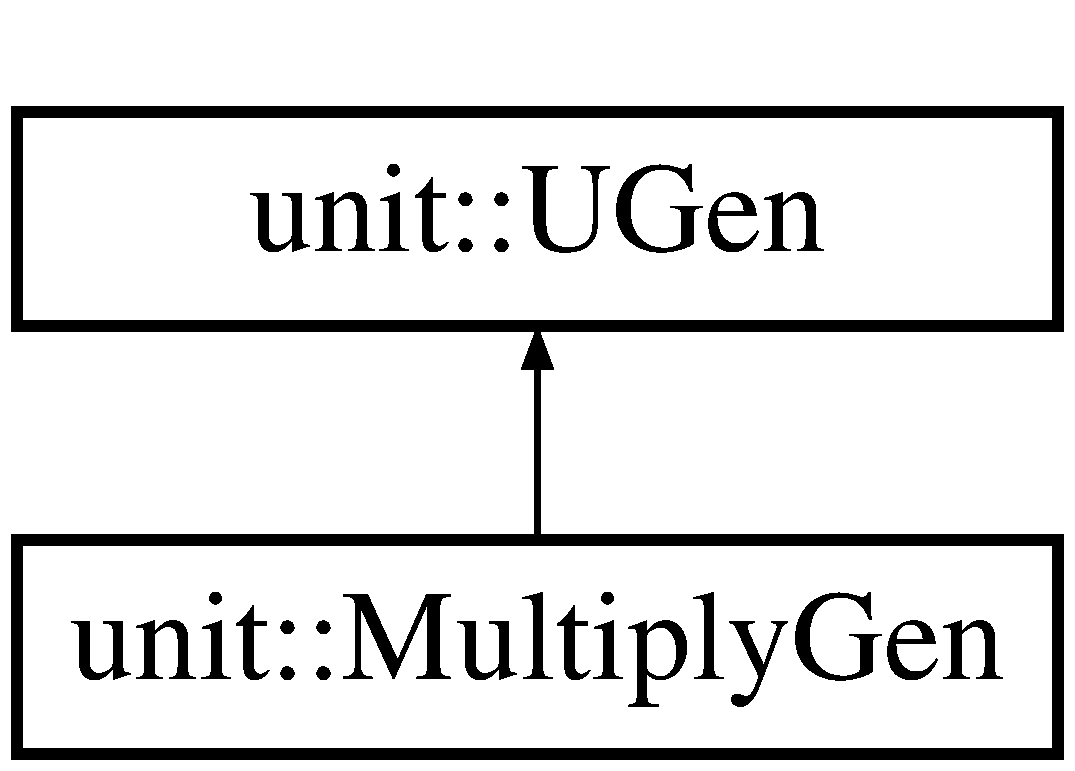
\includegraphics[height=2.000000cm]{classunit_1_1MultiplyGen}
\end{center}
\end{figure}
\subsection*{Public Member Functions}
\begin{DoxyCompactItemize}
\item 
{\bfseries Multiply\+Gen} (std\+::string name)\hypertarget{classunit_1_1MultiplyGen_a8c63aba9e9be634e03f900182b4a1d7a}{}\label{classunit_1_1MultiplyGen_a8c63aba9e9be634e03f900182b4a1d7a}

\item 
void {\bfseries control} (std\+::string port\+Name, float value)\hypertarget{classunit_1_1MultiplyGen_a399981309ef24f24c7044172e58c1e8a}{}\label{classunit_1_1MultiplyGen_a399981309ef24f24c7044172e58c1e8a}

\item 
float {\bfseries tick} ()\hypertarget{classunit_1_1MultiplyGen_abeeb8a84f91375454120639a9bb810fb}{}\label{classunit_1_1MultiplyGen_abeeb8a84f91375454120639a9bb810fb}

\end{DoxyCompactItemize}
\subsection*{Additional Inherited Members}


\subsection{Detailed Description}
\hyperlink{classunit_1_1MultiplyGen}{Multiply\+Gen} is a minimal mixing unit. It multiplies the {\bfseries in1} port with {\bfseries amnt1} port.


\begin{DoxyItemize}
\item {\bfseries tick()} is providing the product of {\bfseries in1} and {\bfseries amnt1}.
\end{DoxyItemize}

Control-\/\+Interface
\begin{DoxyItemize}
\item no control interface implemented
\end{DoxyItemize}

Fast access functions
\begin{DoxyItemize}
\item no further fast access functions implemented
\end{DoxyItemize}

\begin{DoxyAuthor}{Author}
jtm, email\+:  \href{mailto:milde@hs-fulda.de}{\tt milde@hs-\/fulda.\+de} 
\end{DoxyAuthor}
\begin{DoxySince}{Since}
04-\/2016 
\end{DoxySince}
\begin{DoxyVersion}{Version}
1.\+0 
\end{DoxyVersion}


The documentation for this class was generated from the following files\+:\begin{DoxyCompactItemize}
\item 
include/Multiply\+Gen.\+h\item 
unit/Multiply\+Gen.\+cpp\end{DoxyCompactItemize}

\hypertarget{classunit_1_1MultiplyTwoGen}{\section{unit\-:\-:Multiply\-Two\-Gen Class Reference}
\label{classunit_1_1MultiplyTwoGen}\index{unit\-::\-Multiply\-Two\-Gen@{unit\-::\-Multiply\-Two\-Gen}}
}


{\ttfamily \#include $<$Multiply\-Two\-Gen.\-h$>$}

Inheritance diagram for unit\-:\-:Multiply\-Two\-Gen\-:\begin{figure}[H]
\begin{center}
\leavevmode
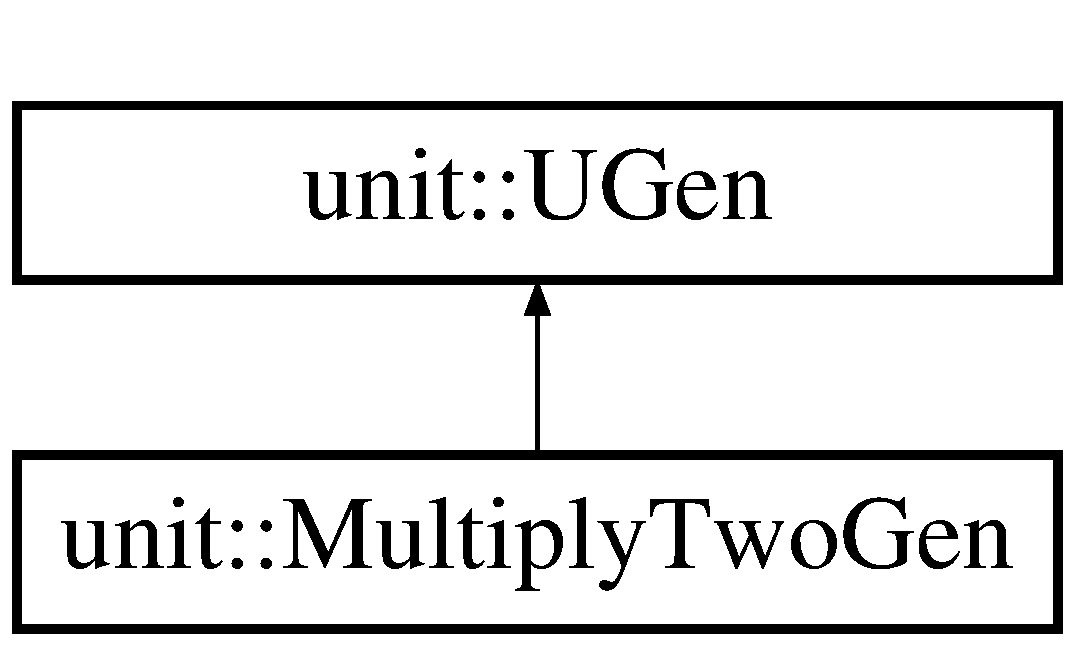
\includegraphics[height=2.000000cm]{classunit_1_1MultiplyTwoGen}
\end{center}
\end{figure}
\subsection*{Public Member Functions}
\begin{DoxyCompactItemize}
\item 
\hypertarget{classunit_1_1MultiplyTwoGen_a35e526170e8ac7a43fc19c2a78e14b44}{{\bfseries Multiply\-Two\-Gen} (std\-::string name)}\label{classunit_1_1MultiplyTwoGen_a35e526170e8ac7a43fc19c2a78e14b44}

\item 
\hypertarget{classunit_1_1MultiplyTwoGen_af8558651a63c73f27221e99ad03f3242}{void {\bfseries control} (std\-::string port\-Name, float value)}\label{classunit_1_1MultiplyTwoGen_af8558651a63c73f27221e99ad03f3242}

\item 
\hypertarget{classunit_1_1MultiplyTwoGen_a70a07ad9e0f67e6a50aadcdf902db8f3}{float {\bfseries tick} ()}\label{classunit_1_1MultiplyTwoGen_a70a07ad9e0f67e6a50aadcdf902db8f3}

\end{DoxyCompactItemize}
\subsection*{Additional Inherited Members}


\subsection{Detailed Description}
\hyperlink{classunit_1_1MultiplyTwoGen}{Multiply\-Two\-Gen} multiplies the two standard input ports in1 and in2.

\begin{DoxyAuthor}{Author}
jtm, email\-:  \href{mailto:milde@hs-fulda.de}{\tt milde@hs-\/fulda.\-de} 
\end{DoxyAuthor}
\begin{DoxySince}{Since}
04-\/2016 
\end{DoxySince}
\begin{DoxyVersion}{Version}
1.\-0 
\end{DoxyVersion}


The documentation for this class was generated from the following files\-:\begin{DoxyCompactItemize}
\item 
include/Multiply\-Two\-Gen.\-h\item 
unit/Multiply\-Two\-Gen.\-cpp\end{DoxyCompactItemize}

\hypertarget{classunit_1_1MultiSwitch5Gen}{\section{unit\-:\-:Multi\-Switch5\-Gen Class Reference}
\label{classunit_1_1MultiSwitch5Gen}\index{unit\-::\-Multi\-Switch5\-Gen@{unit\-::\-Multi\-Switch5\-Gen}}
}


{\ttfamily \#include $<$Multi\-Switch5\-Gen.\-h$>$}

Inheritance diagram for unit\-:\-:Multi\-Switch5\-Gen\-:\begin{figure}[H]
\begin{center}
\leavevmode
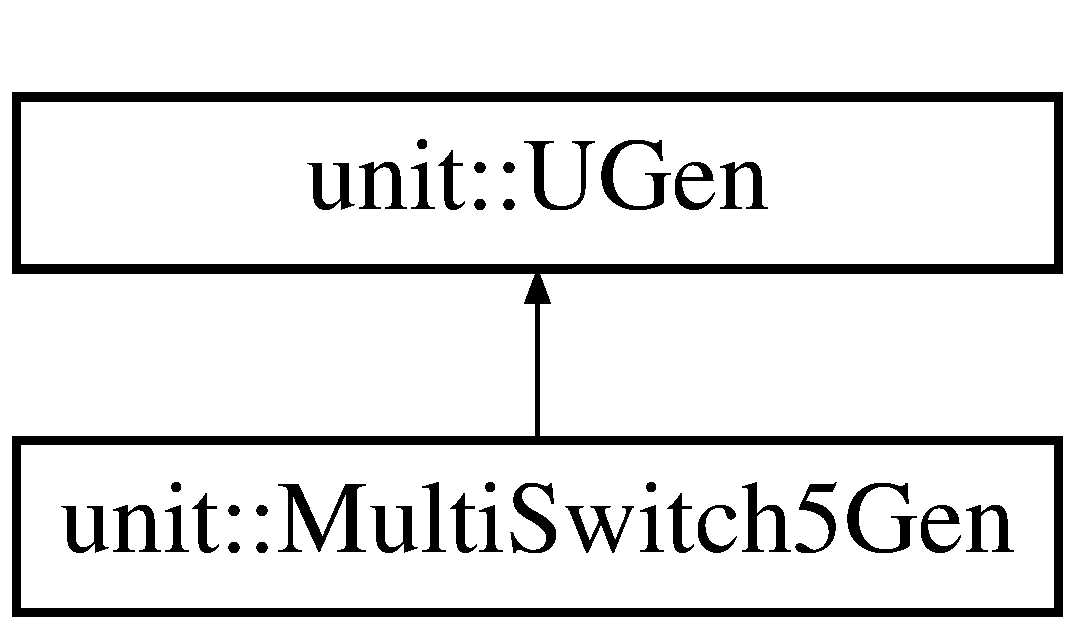
\includegraphics[height=2.000000cm]{classunit_1_1MultiSwitch5Gen}
\end{center}
\end{figure}
\subsection*{Public Member Functions}
\begin{DoxyCompactItemize}
\item 
\hypertarget{classunit_1_1MultiSwitch5Gen_a61feb713c9bf9e11cb7f8da0c27b8faf}{{\bfseries Multi\-Switch5\-Gen} (std\-::string name)}\label{classunit_1_1MultiSwitch5Gen_a61feb713c9bf9e11cb7f8da0c27b8faf}

\item 
\hypertarget{classunit_1_1MultiSwitch5Gen_a22d5724ba74b064282da08c9600bed87}{void {\bfseries control} (std\-::string port\-Name, float value)}\label{classunit_1_1MultiSwitch5Gen_a22d5724ba74b064282da08c9600bed87}

\item 
\hypertarget{classunit_1_1MultiSwitch5Gen_a4c357bd87f34841ccfb6a95f9a820384}{float {\bfseries tick} ()}\label{classunit_1_1MultiSwitch5Gen_a4c357bd87f34841ccfb6a95f9a820384}

\item 
\hypertarget{classunit_1_1MultiSwitch5Gen_ab2c8a47e7d29e01183a02d9fbf60f0ed}{void {\bfseries set\-Select} (float value)}\label{classunit_1_1MultiSwitch5Gen_ab2c8a47e7d29e01183a02d9fbf60f0ed}

\item 
\hypertarget{classunit_1_1MultiSwitch5Gen_a47554a04fc8a495a2ce60ae87460da8d}{void {\bfseries set\-In4} (float value)}\label{classunit_1_1MultiSwitch5Gen_a47554a04fc8a495a2ce60ae87460da8d}

\item 
\hypertarget{classunit_1_1MultiSwitch5Gen_a7073be5cc2e0383aecefdf54c9dec714}{void {\bfseries set\-In5} (float value)}\label{classunit_1_1MultiSwitch5Gen_a7073be5cc2e0383aecefdf54c9dec714}

\item 
\hypertarget{classunit_1_1MultiSwitch5Gen_a97d0f025afcb8b7b5167ccaf244fc9ed}{float {\bfseries get\-In4} ()}\label{classunit_1_1MultiSwitch5Gen_a97d0f025afcb8b7b5167ccaf244fc9ed}

\item 
\hypertarget{classunit_1_1MultiSwitch5Gen_a887395fd9475f73c70b385e3af731828}{float {\bfseries get\-In5} ()}\label{classunit_1_1MultiSwitch5Gen_a887395fd9475f73c70b385e3af731828}

\end{DoxyCompactItemize}
\subsection*{Additional Inherited Members}


\subsection{Detailed Description}
\hyperlink{classunit_1_1MultiSwitch5Gen}{Multi\-Switch5\-Gen} switches between 5 inputs (in1 -\/ in5)

Control-\/\-Interface


\begin{DoxyItemize}
\item control(\char`\"{}select\char`\"{}, value) setzt den select-\/\-Wert \mbox{[}0,1,2,3,4\mbox{]}
\end{DoxyItemize}

\begin{DoxyAuthor}{Author}
jtm 
\end{DoxyAuthor}
\begin{DoxySince}{Since}
04-\/2016 
\end{DoxySince}
\begin{DoxyVersion}{Version}
1.\-0 
\end{DoxyVersion}


The documentation for this class was generated from the following files\-:\begin{DoxyCompactItemize}
\item 
include/Multi\-Switch5\-Gen.\-h\item 
unit/Multi\-Switch5\-Gen.\-cpp\end{DoxyCompactItemize}

\hypertarget{classNeonlicht}{}\section{Neonlicht Class Reference}
\label{classNeonlicht}\index{Neonlicht@{Neonlicht}}
\subsection*{Public Member Functions}
\begin{DoxyCompactItemize}
\item 
void {\bfseries configure} ()\hypertarget{classNeonlicht_a32ec4c221148d01bbafd1637ced9b130}{}\label{classNeonlicht_a32ec4c221148d01bbafd1637ced9b130}

\item 
void {\bfseries start} ()\hypertarget{classNeonlicht_aae54e46be4d251ce4e062cd777994a69}{}\label{classNeonlicht_aae54e46be4d251ce4e062cd777994a69}

\item 
void {\bfseries stop} ()\hypertarget{classNeonlicht_a9d1f643b1a2394f9cd181149f7558c72}{}\label{classNeonlicht_a9d1f643b1a2394f9cd181149f7558c72}

\item 
long {\bfseries get\+Stream\+Latency} ()\hypertarget{classNeonlicht_a4354cc2fa6d7bd22e89d1314e375f54f}{}\label{classNeonlicht_a4354cc2fa6d7bd22e89d1314e375f54f}

\end{DoxyCompactItemize}
\subsection*{Static Public Member Functions}
\begin{DoxyCompactItemize}
\item 
static int {\bfseries tick} (void $\ast$output\+Buffer, void $\ast$input\+Buffer, unsigned int n\+Buffer\+Frames, double stream\+Time, Rt\+Audio\+Stream\+Status status, void $\ast$data\+Pointer)\hypertarget{classNeonlicht_a57c3e8d4154418c9efc4b48d45b732d6}{}\label{classNeonlicht_a57c3e8d4154418c9efc4b48d45b732d6}

\end{DoxyCompactItemize}
\subsection*{Static Public Attributes}
\begin{DoxyCompactItemize}
\item 
static \hyperlink{classCentralStore}{Central\+Store} {\bfseries CS}\hypertarget{classNeonlicht_a1ac3a31190125df3763a9f3d2f085d5e}{}\label{classNeonlicht_a1ac3a31190125df3763a9f3d2f085d5e}

\item 
static int {\bfseries C\+NT} = 0\hypertarget{classNeonlicht_ac86fbdabd4683feaac58b4aefbdf6695}{}\label{classNeonlicht_ac86fbdabd4683feaac58b4aefbdf6695}

\end{DoxyCompactItemize}


The documentation for this class was generated from the following files\+:\begin{DoxyCompactItemize}
\item 
include/Neonlicht.\+h\item 
Neonlicht.\+cpp\end{DoxyCompactItemize}

\hypertarget{classunit_1_1NoiseGen}{}\section{unit\+:\+:Noise\+Gen Class Reference}
\label{classunit_1_1NoiseGen}\index{unit\+::\+Noise\+Gen@{unit\+::\+Noise\+Gen}}


{\ttfamily \#include $<$Noise\+Gen.\+h$>$}

Inheritance diagram for unit\+:\+:Noise\+Gen\+:\begin{figure}[H]
\begin{center}
\leavevmode
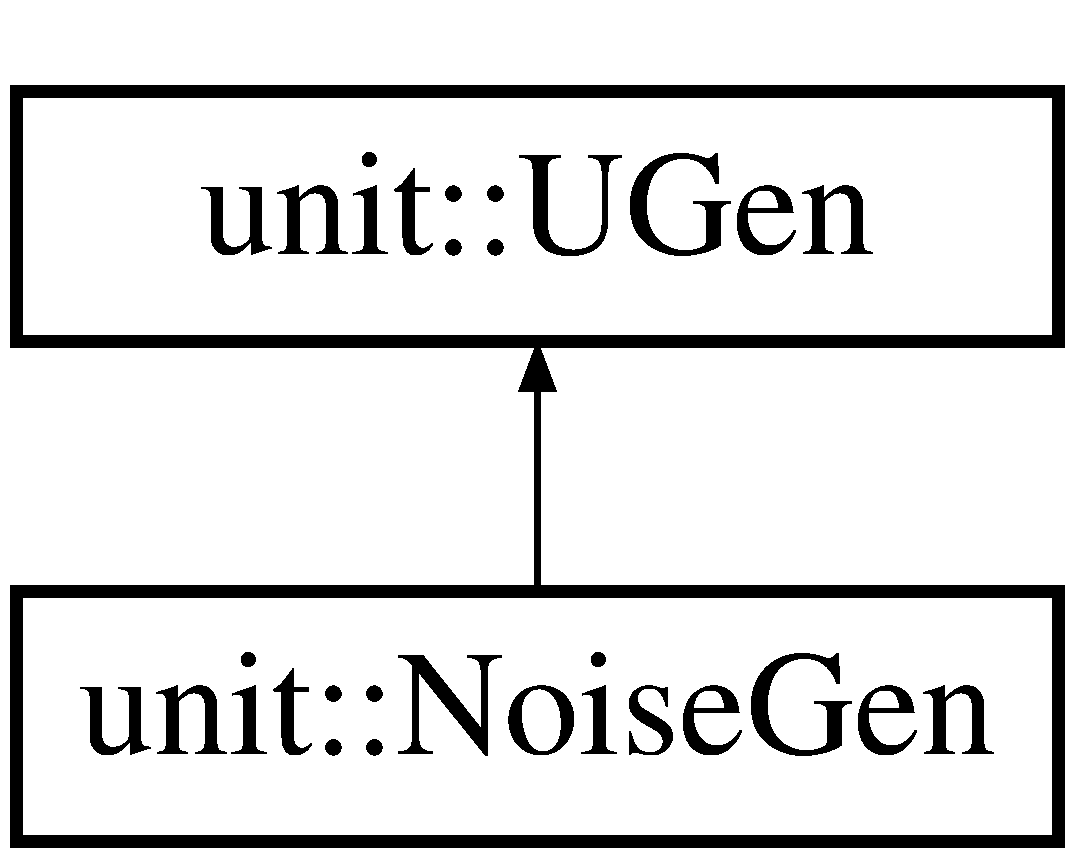
\includegraphics[height=3.000000cm]{classunit_1_1NoiseGen}
\end{center}
\end{figure}
\subsection*{Public Member Functions}
\begin{DoxyCompactItemize}
\item 
{\bfseries Noise\+Gen} (std\+::string name)\hypertarget{classunit_1_1NoiseGen_aa49d8817fff2757abc19f0dffea0c7fe}{}\label{classunit_1_1NoiseGen_aa49d8817fff2757abc19f0dffea0c7fe}

\item 
void {\bfseries control} (std\+::string port\+Name, float value)\hypertarget{classunit_1_1NoiseGen_a73628ae13d893658b88bc30eb43437ba}{}\label{classunit_1_1NoiseGen_a73628ae13d893658b88bc30eb43437ba}

\item 
float {\bfseries tick} ()\hypertarget{classunit_1_1NoiseGen_addaecf96df1cf9f1ba4875fb849949df}{}\label{classunit_1_1NoiseGen_addaecf96df1cf9f1ba4875fb849949df}

\end{DoxyCompactItemize}
\subsection*{Public Attributes}
\begin{DoxyCompactItemize}
\item 
long {\bfseries count} = 0\hypertarget{classunit_1_1NoiseGen_a9509da6dba8e294d3e5bc26d2eb6d39f}{}\label{classunit_1_1NoiseGen_a9509da6dba8e294d3e5bc26d2eb6d39f}

\end{DoxyCompactItemize}
\subsection*{Additional Inherited Members}


\subsection{Detailed Description}
\hyperlink{classunit_1_1NoiseGen}{Noise\+Gen} generates white noise.


\begin{DoxyItemize}
\item {\bfseries tick()} is providing a random value in the range of \mbox{[}-\/1,1\mbox{]}.
\end{DoxyItemize}

Control-\/\+Interface
\begin{DoxyItemize}
\item no control interface implemented
\end{DoxyItemize}

Fast access functions
\begin{DoxyItemize}
\item no further fast access functions implemented
\end{DoxyItemize}

\begin{DoxyAuthor}{Author}
jtm, email\+:  \href{mailto:milde@hs-fulda.de}{\tt milde@hs-\/fulda.\+de} 
\end{DoxyAuthor}
\begin{DoxySince}{Since}
04-\/2016 
\end{DoxySince}
\begin{DoxyVersion}{Version}
1.\+0 
\end{DoxyVersion}


The documentation for this class was generated from the following files\+:\begin{DoxyCompactItemize}
\item 
include/Noise\+Gen.\+h\item 
unit/Noise\+Gen.\+cpp\end{DoxyCompactItemize}

\hypertarget{classNoiseUnit}{}\section{Noise\+Unit Class Reference}
\label{classNoiseUnit}\index{Noise\+Unit@{Noise\+Unit}}
Inheritance diagram for Noise\+Unit\+:\begin{figure}[H]
\begin{center}
\leavevmode
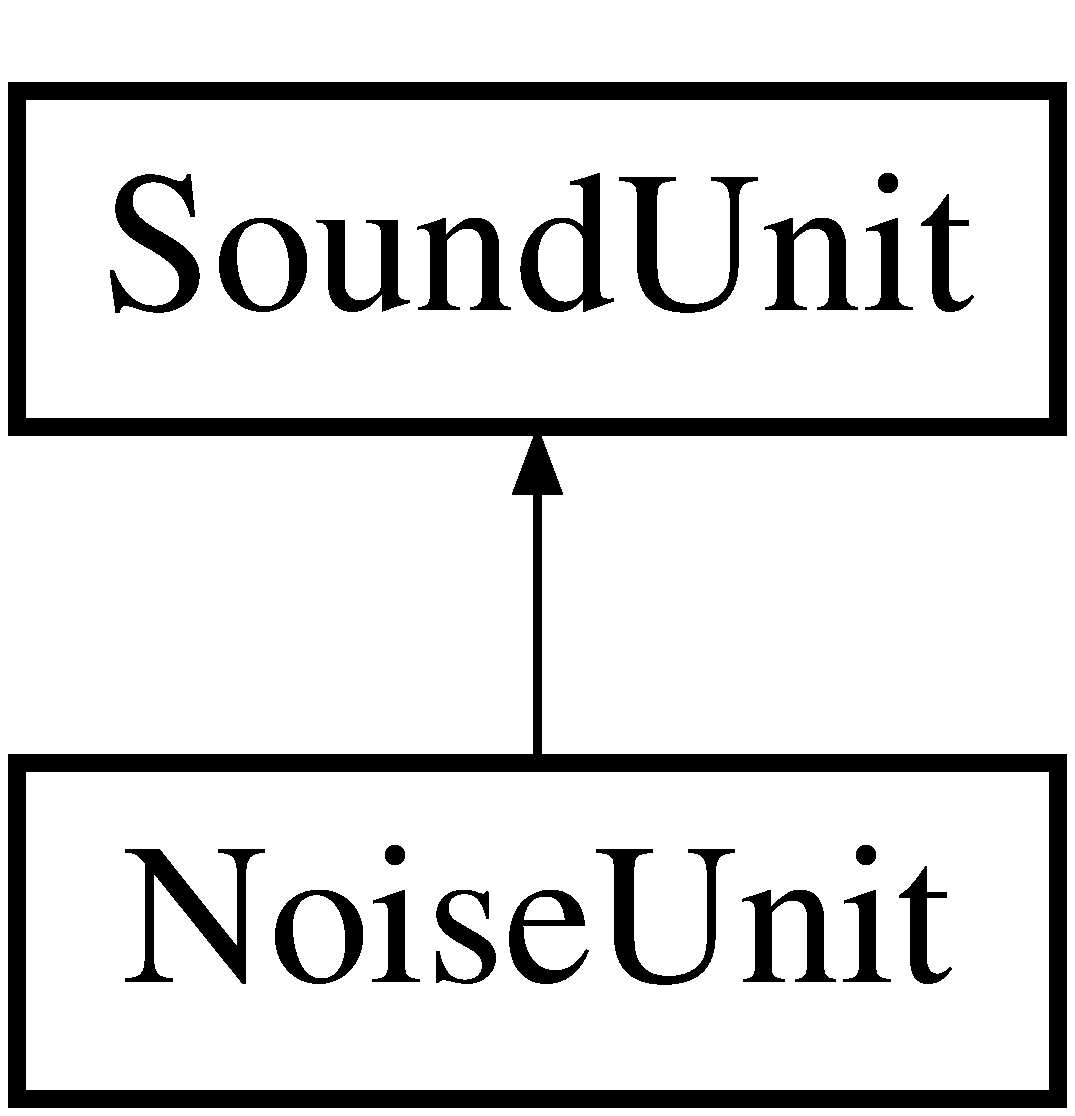
\includegraphics[height=2.000000cm]{classNoiseUnit}
\end{center}
\end{figure}
\subsection*{Public Member Functions}
\begin{DoxyCompactItemize}
\item 
void {\bfseries setup} ()\hypertarget{classNoiseUnit_a81666e8bdea833fad6a4451a765c6b83}{}\label{classNoiseUnit_a81666e8bdea833fad6a4451a765c6b83}

\item 
void {\bfseries control} (std\+::string port\+Name, float value)\hypertarget{classNoiseUnit_a7014ea85fb499bbe69fcf7ce96be8d32}{}\label{classNoiseUnit_a7014ea85fb499bbe69fcf7ce96be8d32}

\item 
float {\bfseries tick} ()\hypertarget{classNoiseUnit_af48a9a915f7f593105e8fe2d2ddb745a}{}\label{classNoiseUnit_af48a9a915f7f593105e8fe2d2ddb745a}

\end{DoxyCompactItemize}
\subsection*{Additional Inherited Members}


The documentation for this class was generated from the following files\+:\begin{DoxyCompactItemize}
\item 
unit/Noise\+Unit.\+h\item 
unit/Noise\+Unit.\+cpp\end{DoxyCompactItemize}

\hypertarget{classunit_1_1NumberGen}{}\section{unit\+:\+:Number\+Gen Class Reference}
\label{classunit_1_1NumberGen}\index{unit\+::\+Number\+Gen@{unit\+::\+Number\+Gen}}


{\ttfamily \#include $<$Number\+Gen.\+h$>$}

Inheritance diagram for unit\+:\+:Number\+Gen\+:\begin{figure}[H]
\begin{center}
\leavevmode
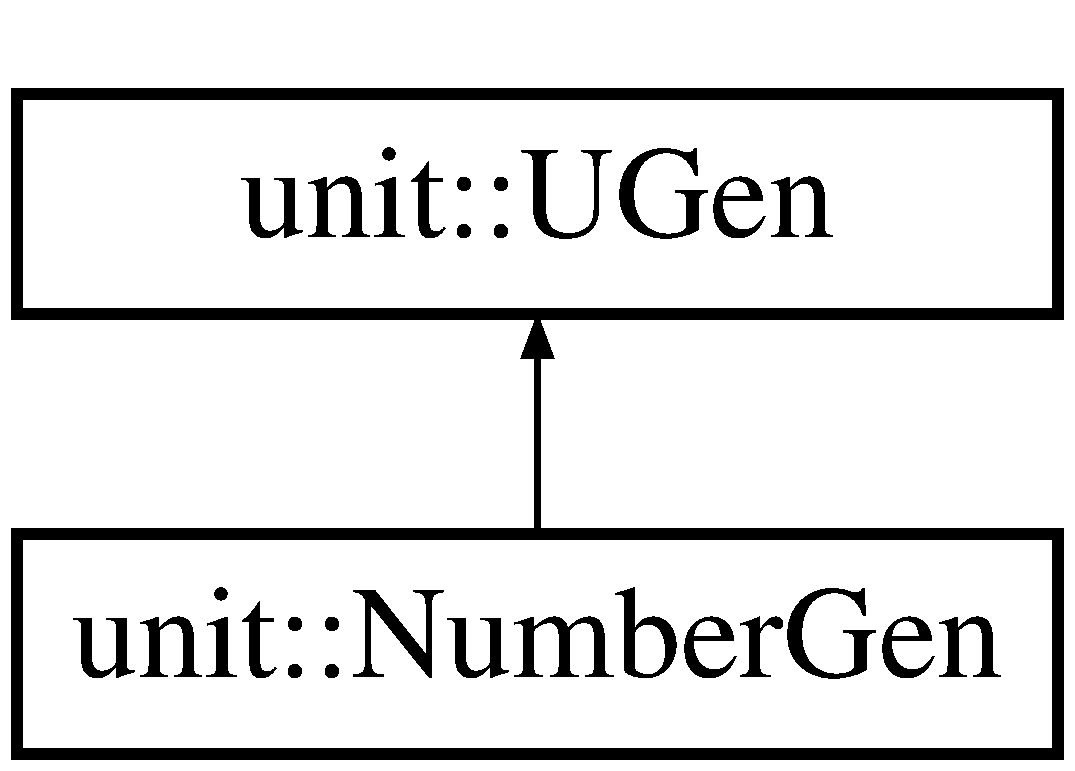
\includegraphics[height=2.000000cm]{classunit_1_1NumberGen}
\end{center}
\end{figure}
\subsection*{Public Member Functions}
\begin{DoxyCompactItemize}
\item 
{\bfseries Number\+Gen} (std\+::string name)\hypertarget{classunit_1_1NumberGen_a6e93812c4805a43f19f8fb11680e32a4}{}\label{classunit_1_1NumberGen_a6e93812c4805a43f19f8fb11680e32a4}

\item 
void {\bfseries control} (std\+::string port\+Name, float value)\hypertarget{classunit_1_1NumberGen_a9daaaf8a12389873494bb1ad2f877c8c}{}\label{classunit_1_1NumberGen_a9daaaf8a12389873494bb1ad2f877c8c}

\item 
float {\bfseries tick} ()\hypertarget{classunit_1_1NumberGen_a38cef7d64a12e40bf2ae14f29def41ca}{}\label{classunit_1_1NumberGen_a38cef7d64a12e40bf2ae14f29def41ca}

\item 
void {\bfseries set\+Value} (float value)\hypertarget{classunit_1_1NumberGen_ad5c107c90a5bc6cf7bbc39562db9d9e3}{}\label{classunit_1_1NumberGen_ad5c107c90a5bc6cf7bbc39562db9d9e3}

\end{DoxyCompactItemize}
\subsection*{Additional Inherited Members}


\subsection{Detailed Description}
\hyperlink{classunit_1_1NumberGen}{Number\+Gen} stores a value.


\begin{DoxyItemize}
\item {\bfseries tick()} is providing the stored value.
\end{DoxyItemize}

Control-\/\+Interface -\/$\ast$$\ast$control(\char`\"{}non empty string\char`\"{}, value)$\ast$$\ast$\+: stores the value in amnt1. The port\+Name has to be a non empty string, otherwise the value will not be stored.

Fast access functions
\begin{DoxyItemize}
\item {\bfseries set\+Value(float value)}\+: stores the value in amnt1 (and in out1).
\end{DoxyItemize}

\begin{DoxyAuthor}{Author}
jtm, email\+:  \href{mailto:milde@hs-fulda.de}{\tt milde@hs-\/fulda.\+de} 
\end{DoxyAuthor}
\begin{DoxySince}{Since}
04-\/2016 
\end{DoxySince}
\begin{DoxyVersion}{Version}
1.\+0 
\end{DoxyVersion}


The documentation for this class was generated from the following files\+:\begin{DoxyCompactItemize}
\item 
include/Number\+Gen.\+h\item 
unit/Number\+Gen.\+cpp\end{DoxyCompactItemize}

\hypertarget{classunit_1_1OnePoleLPFGen}{}\section{unit\+:\+:One\+Pole\+L\+P\+F\+Gen Class Reference}
\label{classunit_1_1OnePoleLPFGen}\index{unit\+::\+One\+Pole\+L\+P\+F\+Gen@{unit\+::\+One\+Pole\+L\+P\+F\+Gen}}
Inheritance diagram for unit\+:\+:One\+Pole\+L\+P\+F\+Gen\+:\begin{figure}[H]
\begin{center}
\leavevmode
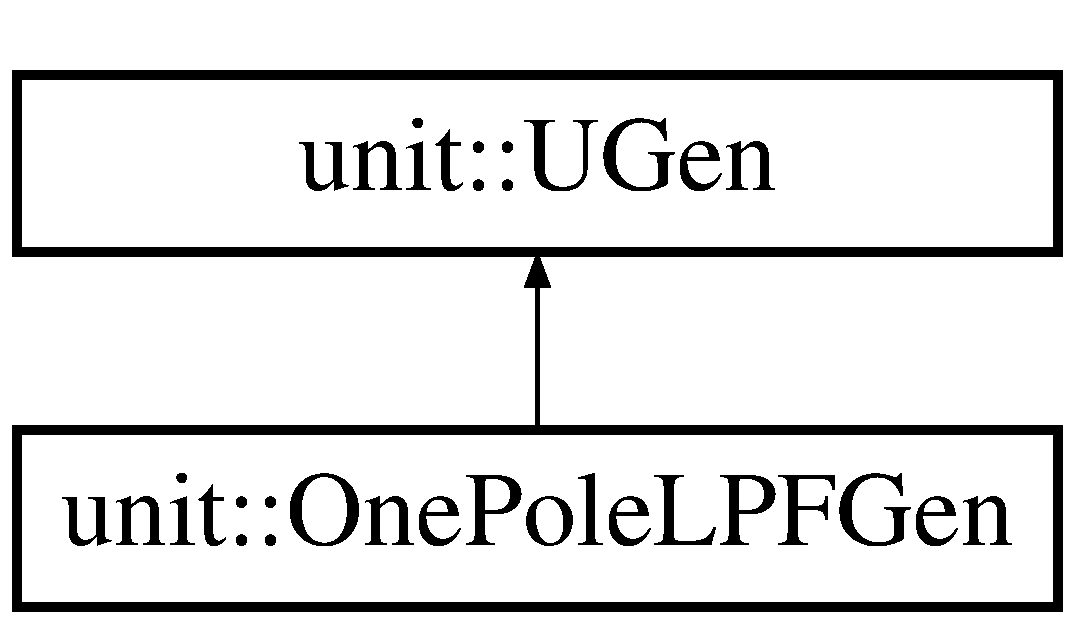
\includegraphics[height=2.000000cm]{classunit_1_1OnePoleLPFGen}
\end{center}
\end{figure}
\subsection*{Public Member Functions}
\begin{DoxyCompactItemize}
\item 
{\bfseries One\+Pole\+L\+P\+F\+Gen} (std\+::string name)\hypertarget{classunit_1_1OnePoleLPFGen_aea39a9562852ac47fdd576fd8b583b9f}{}\label{classunit_1_1OnePoleLPFGen_aea39a9562852ac47fdd576fd8b583b9f}

\item 
void {\bfseries control} (std\+::string port\+Name, float value)\hypertarget{classunit_1_1OnePoleLPFGen_a8f2df9b7406edadf7dc34e7e65b2b67c}{}\label{classunit_1_1OnePoleLPFGen_a8f2df9b7406edadf7dc34e7e65b2b67c}

\item 
float {\bfseries tick} ()\hypertarget{classunit_1_1OnePoleLPFGen_a5e5288841ff8112113f2d6ec1f03f375}{}\label{classunit_1_1OnePoleLPFGen_a5e5288841ff8112113f2d6ec1f03f375}

\end{DoxyCompactItemize}
\subsection*{Additional Inherited Members}


The documentation for this class was generated from the following files\+:\begin{DoxyCompactItemize}
\item 
unit/One\+Pole\+L\+P\+F\+Gen.\+h\item 
unit/One\+Pole\+L\+P\+F\+Gen.\+cpp\end{DoxyCompactItemize}

\hypertarget{classOscActivator}{}\section{Osc\+Activator Class Reference}
\label{classOscActivator}\index{Osc\+Activator@{Osc\+Activator}}
Inheritance diagram for Osc\+Activator\+:\begin{figure}[H]
\begin{center}
\leavevmode
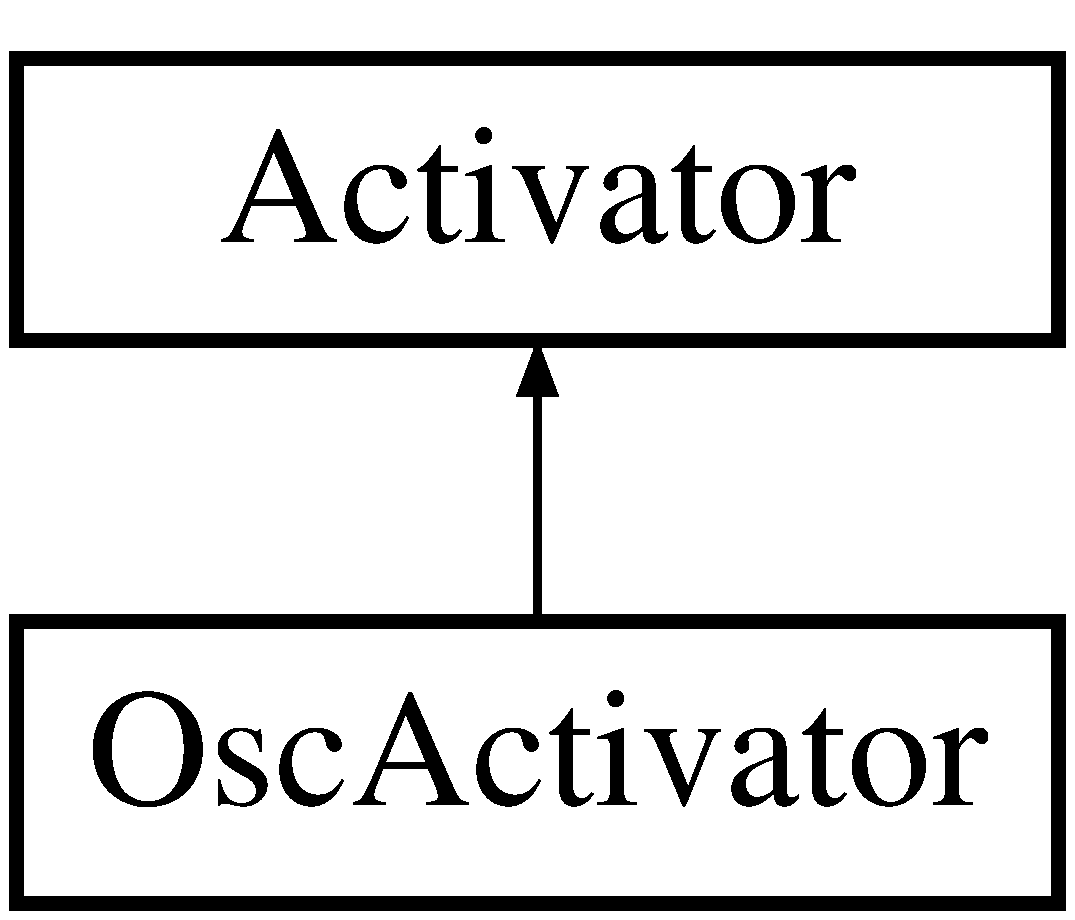
\includegraphics[height=2.000000cm]{classOscActivator}
\end{center}
\end{figure}
\subsection*{Public Member Functions}
\begin{DoxyCompactItemize}
\item 
void {\bfseries callback} (float value)\hypertarget{classOscActivator_ad5852376e949408b2fc13c8adf60c032}{}\label{classOscActivator_ad5852376e949408b2fc13c8adf60c032}

\end{DoxyCompactItemize}


The documentation for this class was generated from the following files\+:\begin{DoxyCompactItemize}
\item 
sequencer/Osc\+Activator.\+h\item 
sequencer/Osc\+Activator.\+cpp\end{DoxyCompactItemize}

\hypertarget{classunit_1_1OscillatorGen}{\section{unit\-:\-:Oscillator\-Gen Class Reference}
\label{classunit_1_1OscillatorGen}\index{unit\-::\-Oscillator\-Gen@{unit\-::\-Oscillator\-Gen}}
}


{\ttfamily \#include $<$Oscillator\-Gen.\-h$>$}

Inheritance diagram for unit\-:\-:Oscillator\-Gen\-:\begin{figure}[H]
\begin{center}
\leavevmode
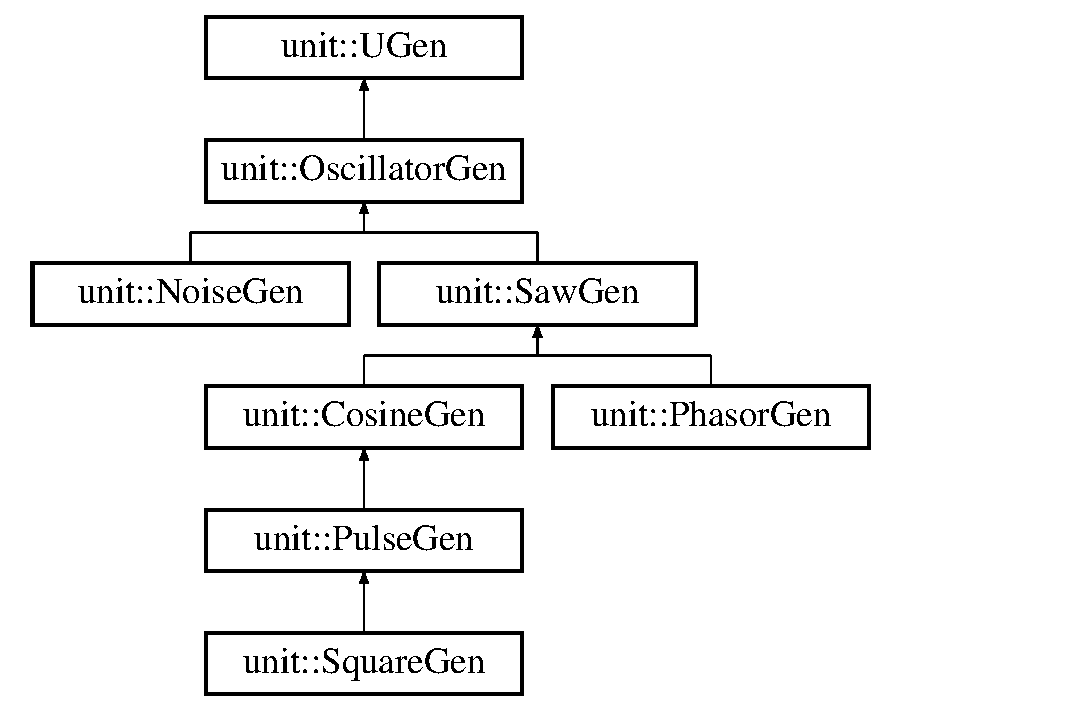
\includegraphics[height=6.000000cm]{classunit_1_1OscillatorGen}
\end{center}
\end{figure}
\subsection*{Public Member Functions}
\begin{DoxyCompactItemize}
\item 
\hypertarget{classunit_1_1OscillatorGen_ab84067cdd1c0a20d238ddcaaadda12da}{{\bfseries Oscillator\-Gen} (std\-::string name)}\label{classunit_1_1OscillatorGen_ab84067cdd1c0a20d238ddcaaadda12da}

\end{DoxyCompactItemize}
\subsection*{Additional Inherited Members}


\subsection{Detailed Description}
\hyperlink{classunit_1_1OscillatorGen}{Oscillator\-Gen} is an intermedediate class and serves as a general base class for all oscillators.

\begin{DoxyAuthor}{Author}
jtm, email\-:  \href{mailto:milde@hs-fulda.de}{\tt milde@hs-\/fulda.\-de} 
\end{DoxyAuthor}
\begin{DoxySince}{Since}
04-\/2016 
\end{DoxySince}
\begin{DoxyVersion}{Version}
1.\-0 
\end{DoxyVersion}


The documentation for this class was generated from the following files\-:\begin{DoxyCompactItemize}
\item 
src/include/Oscillator\-Gen.\-h\item 
src/unit/Oscillator\-Gen.\-cpp\end{DoxyCompactItemize}

\hypertarget{classosc_1_1OscInConnector}{\section{osc\-:\-:Osc\-In\-Connector Class Reference}
\label{classosc_1_1OscInConnector}\index{osc\-::\-Osc\-In\-Connector@{osc\-::\-Osc\-In\-Connector}}
}
\subsection*{Classes}
\begin{DoxyCompactItemize}
\item 
class \hyperlink{classOscInConnector_1_1MidiPacketListener}{Midi\-Packet\-Listener}
\end{DoxyCompactItemize}
\subsection*{Public Member Functions}
\begin{DoxyCompactItemize}
\item 
\hypertarget{classosc_1_1OscInConnector_acb8cca9cec941690ed0dcee6611c4553}{{\bfseries Osc\-In\-Connector} (int prt)}\label{classosc_1_1OscInConnector_acb8cca9cec941690ed0dcee6611c4553}

\item 
\hypertarget{classosc_1_1OscInConnector_a6603048c9ba0e9356a8dd0f5ffc1055f}{bool {\bfseries is\-Fresh} ()}\label{classosc_1_1OscInConnector_a6603048c9ba0e9356a8dd0f5ffc1055f}

\item 
\hypertarget{classosc_1_1OscInConnector_aa7130d46061b498d0f8648c0bd9c4146}{\hyperlink{classosc_1_1MessageData}{Message\-Data} $\ast$ {\bfseries get\-Data} ()}\label{classosc_1_1OscInConnector_aa7130d46061b498d0f8648c0bd9c4146}

\item 
std\-::thread \hyperlink{classosc_1_1OscInConnector_af546d19cf2adc1ed7c701a4804586cb9}{start\-Thread} ()
\end{DoxyCompactItemize}
\subsection*{Public Attributes}
\begin{DoxyCompactItemize}
\item 
\hypertarget{classosc_1_1OscInConnector_a1fd59b88007b9942b275aaa1f6c7bbc1}{\hyperlink{classosc_1_1MessageData}{Message\-Data} $\ast$ {\bfseries M\-D} = new \hyperlink{classosc_1_1MessageData}{Message\-Data}(\char`\"{}xxx\char`\"{},1,2,3,3.\-14f)}\label{classosc_1_1OscInConnector_a1fd59b88007b9942b275aaa1f6c7bbc1}

\item 
\hypertarget{classosc_1_1OscInConnector_a8a88a1532af47166b8e7c91da8d47662}{bool {\bfseries talk} = true}\label{classosc_1_1OscInConnector_a8a88a1532af47166b8e7c91da8d47662}

\end{DoxyCompactItemize}


\subsection{Member Function Documentation}
\hypertarget{classosc_1_1OscInConnector_af546d19cf2adc1ed7c701a4804586cb9}{\index{osc\-::\-Osc\-In\-Connector@{osc\-::\-Osc\-In\-Connector}!start\-Thread@{start\-Thread}}
\index{start\-Thread@{start\-Thread}!osc::OscInConnector@{osc\-::\-Osc\-In\-Connector}}
\subsubsection[{start\-Thread}]{\setlength{\rightskip}{0pt plus 5cm}std\-::thread Osc\-In\-Connector\-::start\-Thread (
\begin{DoxyParamCaption}
{}
\end{DoxyParamCaption}
)}}\label{classosc_1_1OscInConnector_af546d19cf2adc1ed7c701a4804586cb9}
Scheint zu funktionieren, keine Ahnung warum \-:) 

The documentation for this class was generated from the following files\-:\begin{DoxyCompactItemize}
\item 
include/Osc\-In\-Connector.\-h\item 
osc/Osc\-In\-Connector.\-cpp\end{DoxyCompactItemize}

\hypertarget{classosc_1_1OscOutConnector}{\section{osc\-:\-:Osc\-Out\-Connector Class Reference}
\label{classosc_1_1OscOutConnector}\index{osc\-::\-Osc\-Out\-Connector@{osc\-::\-Osc\-Out\-Connector}}
}
\subsection*{Public Member Functions}
\begin{DoxyCompactItemize}
\item 
\hypertarget{classosc_1_1OscOutConnector_a7dde00203135c4a673e56f02dec774b4}{{\bfseries Osc\-Out\-Connector} (std\-::string h, int p)}\label{classosc_1_1OscOutConnector_a7dde00203135c4a673e56f02dec774b4}

\item 
\hypertarget{classosc_1_1OscOutConnector_a8b3bcadf0295998b42753161ae9d17ee}{void {\bfseries send\-Message} (std\-::string s, int a1, int a2, int a3, float f1)}\label{classosc_1_1OscOutConnector_a8b3bcadf0295998b42753161ae9d17ee}

\end{DoxyCompactItemize}


The documentation for this class was generated from the following files\-:\begin{DoxyCompactItemize}
\item 
include/Osc\-Out\-Connector.\-h\item 
osc/Osc\-Out\-Connector.\-cpp\end{DoxyCompactItemize}

\hypertarget{classOscWrapper}{\section{Osc\-Wrapper Class Reference}
\label{classOscWrapper}\index{Osc\-Wrapper@{Osc\-Wrapper}}
}


The documentation for this class was generated from the following files\-:\begin{DoxyCompactItemize}
\item 
include/Osc\-Wrapper.\-h\item 
store/Osc\-Wrapper.\-cpp\end{DoxyCompactItemize}

\hypertarget{classPatch}{}\section{Patch Class Reference}
\label{classPatch}\index{Patch@{Patch}}
\subsection*{Public Member Functions}
\begin{DoxyCompactItemize}
\item 
{\bfseries Patch} (std\+::string from, int pt\+From, std\+::string to, int p\+To)\hypertarget{classPatch_a5ff9de0f83c44aa11aae837870aa55f0}{}\label{classPatch_a5ff9de0f83c44aa11aae837870aa55f0}

\item 
std\+::string {\bfseries get\+From} ()\hypertarget{classPatch_a97b08ef9e08c5ef8b5d71692a7242796}{}\label{classPatch_a97b08ef9e08c5ef8b5d71692a7242796}

\item 
int {\bfseries get\+From\+Port} ()\hypertarget{classPatch_a365988c401459bfd0f0b5b21f041bfe1}{}\label{classPatch_a365988c401459bfd0f0b5b21f041bfe1}

\item 
std\+::string {\bfseries get\+To} ()\hypertarget{classPatch_ade1fb3107faa8224f29c4a8387821fee}{}\label{classPatch_ade1fb3107faa8224f29c4a8387821fee}

\item 
int {\bfseries get\+Form\+Port} ()\hypertarget{classPatch_a19e489d67f86b80ac5f0ef774a3b87c8}{}\label{classPatch_a19e489d67f86b80ac5f0ef774a3b87c8}

\end{DoxyCompactItemize}


The documentation for this class was generated from the following files\+:\begin{DoxyCompactItemize}
\item 
unit/Patch.\+h\item 
unit/Patch.\+cpp\end{DoxyCompactItemize}

\hypertarget{classunit_1_1PhasorGen}{\section{unit\-:\-:Phasor\-Gen Class Reference}
\label{classunit_1_1PhasorGen}\index{unit\-::\-Phasor\-Gen@{unit\-::\-Phasor\-Gen}}
}


{\ttfamily \#include $<$Phasor\-Gen.\-h$>$}

Inheritance diagram for unit\-:\-:Phasor\-Gen\-:\begin{figure}[H]
\begin{center}
\leavevmode
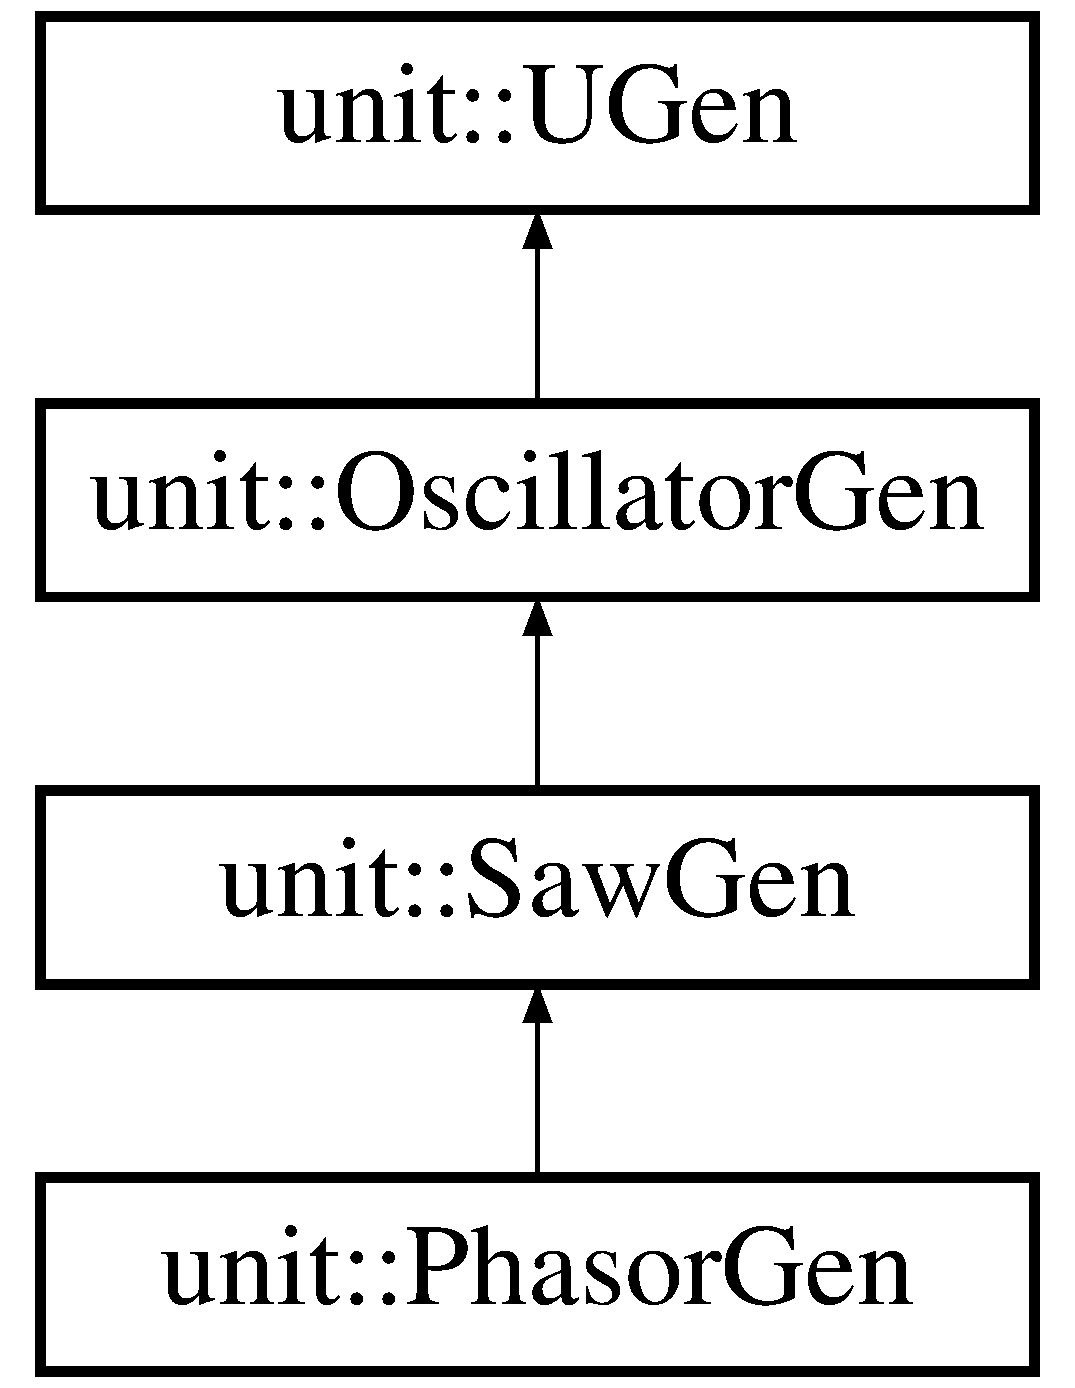
\includegraphics[height=4.000000cm]{classunit_1_1PhasorGen}
\end{center}
\end{figure}
\subsection*{Public Member Functions}
\begin{DoxyCompactItemize}
\item 
\hypertarget{classunit_1_1PhasorGen_a726fab6730e45d7fbf242f4613837e28}{{\bfseries Phasor\-Gen} (std\-::string name)}\label{classunit_1_1PhasorGen_a726fab6730e45d7fbf242f4613837e28}

\item 
\hypertarget{classunit_1_1PhasorGen_a056953090628af9868e4778d15daf79a}{float {\bfseries tick} ()}\label{classunit_1_1PhasorGen_a056953090628af9868e4778d15daf79a}

\end{DoxyCompactItemize}
\subsection*{Additional Inherited Members}


\subsection{Detailed Description}
\hyperlink{classunit_1_1PhasorGen}{Phasor\-Gen} generates a standard ramp \mbox{[}0,1\mbox{]}.

\begin{DoxyAuthor}{Author}
jtm, email\-:  \href{mailto:milde@hs-fulda.de}{\tt milde@hs-\/fulda.\-de} 
\end{DoxyAuthor}
\begin{DoxySince}{Since}
04-\/2016 
\end{DoxySince}
\begin{DoxyVersion}{Version}
1.\-0 
\end{DoxyVersion}


The documentation for this class was generated from the following files\-:\begin{DoxyCompactItemize}
\item 
src/include/Phasor\-Gen.\-h\item 
src/unit/Phasor\-Gen.\-cpp\end{DoxyCompactItemize}

\hypertarget{classPort}{\section{Port Class Reference}
\label{classPort}\index{Port@{Port}}
}
\subsection*{Public Member Functions}
\begin{DoxyCompactItemize}
\item 
\hypertarget{classPort_aadff8efe873e31b3362dda2b4a28c8c9}{{\bfseries Port} (std\-::string name, Port\-Type t)}\label{classPort_aadff8efe873e31b3362dda2b4a28c8c9}

\item 
\hypertarget{classPort_ad2c3baf0b291aee3b5b65178231754a6}{std\-::string {\bfseries get\-Name} ()}\label{classPort_ad2c3baf0b291aee3b5b65178231754a6}

\item 
\hypertarget{classPort_a31744528a5ade68a59ce094f3797bc1e}{std\-::string {\bfseries get\-I\-D} ()}\label{classPort_a31744528a5ade68a59ce094f3797bc1e}

\item 
\hypertarget{classPort_a5859f5d788d56c0103f4274b6d62b725}{Port\-Type {\bfseries get\-Type} ()}\label{classPort_a5859f5d788d56c0103f4274b6d62b725}

\item 
\hypertarget{classPort_a101b9cfba62777fb61c35a642b63f25a}{float {\bfseries get\-Value} ()}\label{classPort_a101b9cfba62777fb61c35a642b63f25a}

\item 
\hypertarget{classPort_afc93a217ba756e559c157b66745823a7}{void {\bfseries set\-Value} (float v)}\label{classPort_afc93a217ba756e559c157b66745823a7}

\end{DoxyCompactItemize}


The documentation for this class was generated from the following files\-:\begin{DoxyCompactItemize}
\item 
src/include/Port.\-h\item 
src/unit/Port.\-cpp\end{DoxyCompactItemize}

\hypertarget{classPulse}{\section{Pulse Class Reference}
\label{classPulse}\index{Pulse@{Pulse}}
}


{\ttfamily \#include $<$Pulse.\-h$>$}

\subsection*{Public Member Functions}
\begin{DoxyCompactItemize}
\item 
\hypertarget{classPulse_a9835b637db766732dd508c94fc30c501}{{\bfseries Pulse} (float bpm)}\label{classPulse_a9835b637db766732dd508c94fc30c501}

\item 
\hypertarget{classPulse_a164d81d4e1e798a5eec15b0b030b4047}{void {\bfseries start} ()}\label{classPulse_a164d81d4e1e798a5eec15b0b030b4047}

\item 
\hypertarget{classPulse_a7c8121986bec5319bb097216fe5e93d0}{void {\bfseries stop} ()}\label{classPulse_a7c8121986bec5319bb097216fe5e93d0}

\item 
\hypertarget{classPulse_a8283f4ab252e0c38b1e19a4dec522f23}{void {\bfseries set\-Activator} (\hyperlink{classActivator}{Activator} $\ast$a)}\label{classPulse_a8283f4ab252e0c38b1e19a4dec522f23}

\item 
\hypertarget{classPulse_afc87b2e4120c47942cf03fc82aaf8002}{void {\bfseries set\-Speed} (float bpm)}\label{classPulse_afc87b2e4120c47942cf03fc82aaf8002}

\end{DoxyCompactItemize}


\subsection{Detailed Description}
\hyperlink{classPulse}{Pulse} generates a beat and sends the pulses to an \hyperlink{classActivator}{Activator}. The pulse is quantized to a zweiundreissigstel (thirty second note/demisemiquaver).

\begin{DoxyAuthor}{Author}
jtm, email\-:  \href{mailto:milde@hs-fulda.de}{\tt milde@hs-\/fulda.\-de} 
\end{DoxyAuthor}
\begin{DoxySince}{Since}
04-\/2016 
\end{DoxySince}
\begin{DoxyVersion}{Version}
1.\-0 
\end{DoxyVersion}


The documentation for this class was generated from the following files\-:\begin{DoxyCompactItemize}
\item 
include/Pulse.\-h\item 
sequencer/Pulse.\-cpp\end{DoxyCompactItemize}

\hypertarget{classunit_1_1PulseGen}{}\section{unit\+:\+:Pulse\+Gen Class Reference}
\label{classunit_1_1PulseGen}\index{unit\+::\+Pulse\+Gen@{unit\+::\+Pulse\+Gen}}
Inheritance diagram for unit\+:\+:Pulse\+Gen\+:\begin{figure}[H]
\begin{center}
\leavevmode
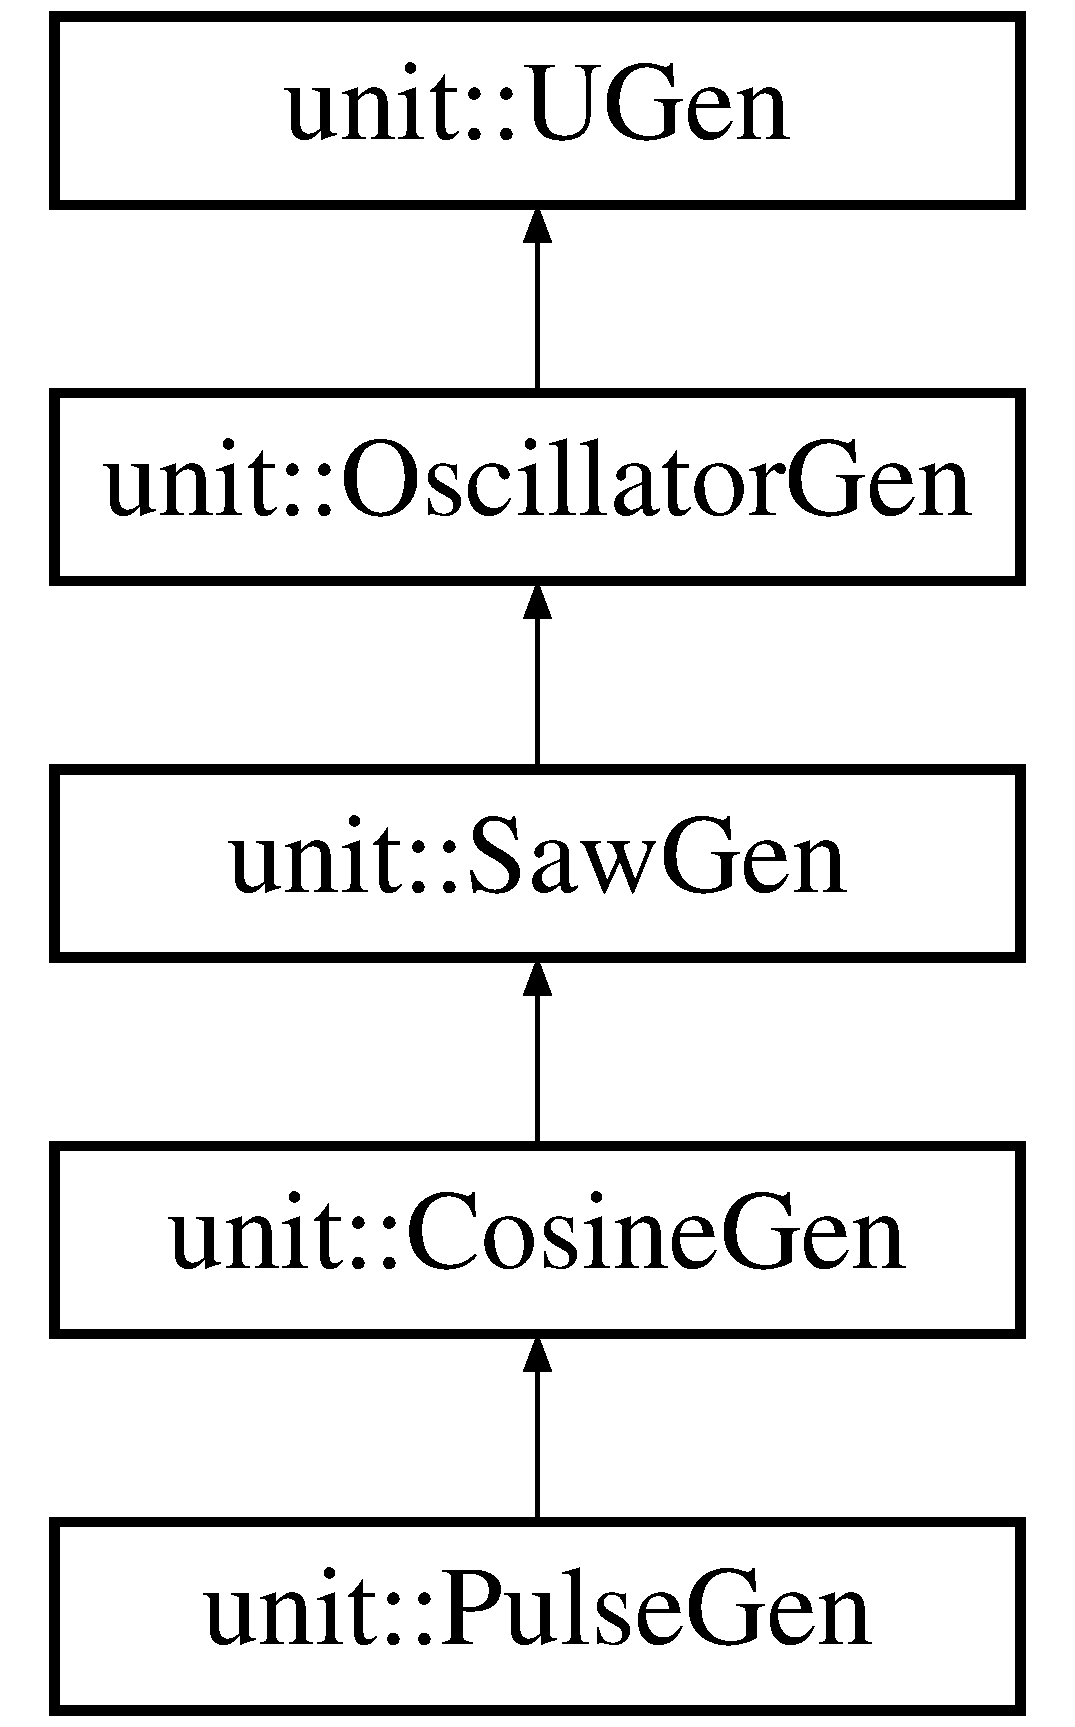
\includegraphics[height=5.000000cm]{classunit_1_1PulseGen}
\end{center}
\end{figure}
\subsection*{Public Member Functions}
\begin{DoxyCompactItemize}
\item 
{\bfseries Pulse\+Gen} (std\+::string name)\hypertarget{classunit_1_1PulseGen_a466bdb3fcc244e66f2c29a9a517d4b85}{}\label{classunit_1_1PulseGen_a466bdb3fcc244e66f2c29a9a517d4b85}

\item 
float {\bfseries tick} ()\hypertarget{classunit_1_1PulseGen_a8b09b8d3cf11eb6a315bdd9b6347227d}{}\label{classunit_1_1PulseGen_a8b09b8d3cf11eb6a315bdd9b6347227d}

\item 
void {\bfseries control} (std\+::string port\+Name, float value)\hypertarget{classunit_1_1PulseGen_a581c649900c094728f4b587fb36c4f56}{}\label{classunit_1_1PulseGen_a581c649900c094728f4b587fb36c4f56}

\item 
void {\bfseries set\+Frequency} (float value)\hypertarget{classunit_1_1PulseGen_af4a027e50251040d914cdf18a87d7a73}{}\label{classunit_1_1PulseGen_af4a027e50251040d914cdf18a87d7a73}

\item 
float {\bfseries get\+Frequency} ()\hypertarget{classunit_1_1PulseGen_aa4b24157a5f5a95d1ccf0cf639598b8f}{}\label{classunit_1_1PulseGen_aa4b24157a5f5a95d1ccf0cf639598b8f}

\item 
void {\bfseries set\+Pulse\+Width} (float value)\hypertarget{classunit_1_1PulseGen_a9be5874432ee5e966542bc1b568faa61}{}\label{classunit_1_1PulseGen_a9be5874432ee5e966542bc1b568faa61}

\end{DoxyCompactItemize}
\subsection*{Additional Inherited Members}


The documentation for this class was generated from the following files\+:\begin{DoxyCompactItemize}
\item 
unit/Pulse\+Gen.\+h\item 
unit/Pulse\+Gen.\+cpp\end{DoxyCompactItemize}

\hypertarget{classunit_1_1SawGen}{\section{unit\-:\-:Saw\-Gen Class Reference}
\label{classunit_1_1SawGen}\index{unit\-::\-Saw\-Gen@{unit\-::\-Saw\-Gen}}
}


{\ttfamily \#include $<$Saw\-Gen.\-h$>$}

Inheritance diagram for unit\-:\-:Saw\-Gen\-:\begin{figure}[H]
\begin{center}
\leavevmode
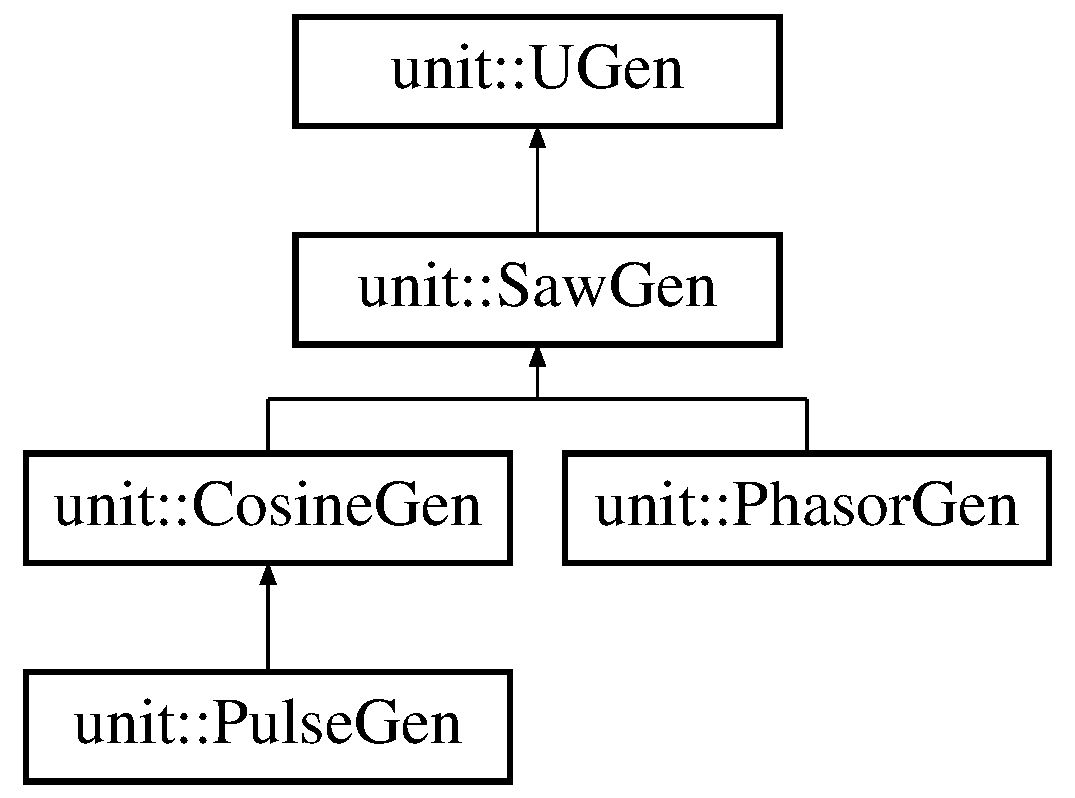
\includegraphics[height=6.000000cm]{classunit_1_1SawGen}
\end{center}
\end{figure}
\subsection*{Public Member Functions}
\begin{DoxyCompactItemize}
\item 
\hypertarget{classunit_1_1SawGen_a24c35afc1bdb237a8a5d1eb3888ce0bc}{{\bfseries Saw\-Gen} (std\-::string name)}\label{classunit_1_1SawGen_a24c35afc1bdb237a8a5d1eb3888ce0bc}

\item 
\hypertarget{classunit_1_1SawGen_a515f6eb82a1a97ee434144b8c58133b8}{void {\bfseries control} (std\-::string port\-Name, float value)}\label{classunit_1_1SawGen_a515f6eb82a1a97ee434144b8c58133b8}

\item 
\hypertarget{classunit_1_1SawGen_a18c6704aec8f20a5605ff72d674c7516}{float {\bfseries tick} ()}\label{classunit_1_1SawGen_a18c6704aec8f20a5605ff72d674c7516}

\item 
\hypertarget{classunit_1_1SawGen_a1a77058c93e7f7b3fe4b355953674678}{void {\bfseries set\-Frequency} (float value)}\label{classunit_1_1SawGen_a1a77058c93e7f7b3fe4b355953674678}

\item 
\hypertarget{classunit_1_1SawGen_a0f08973bebb28aa1a059ccce09e5ebdf}{float {\bfseries get\-Frequency} ()}\label{classunit_1_1SawGen_a0f08973bebb28aa1a059ccce09e5ebdf}

\end{DoxyCompactItemize}
\subsection*{Additional Inherited Members}


\subsection{Detailed Description}
\hyperlink{classunit_1_1SawGen}{Saw\-Gen} generates a saw wave based on a simple linear interpolation.

The implementation is not very effective and needs to be redone. It also contains an implementation error. It should use a wave table.

\begin{DoxyAuthor}{Author}
jtm, email\-:  \href{mailto:milde@hs-fulda.de}{\tt milde@hs-\/fulda.\-de} 
\end{DoxyAuthor}
\begin{DoxySince}{Since}
04-\/2016 
\end{DoxySince}
\begin{DoxyVersion}{Version}
1.\-0 
\end{DoxyVersion}


The documentation for this class was generated from the following files\-:\begin{DoxyCompactItemize}
\item 
include/Saw\-Gen.\-h\item 
unit/Saw\-Gen.\-cpp\end{DoxyCompactItemize}

\hypertarget{classCONFIG4CPP__NAMESPACE_1_1SchemaIdRuleInfo}{\section{C\-O\-N\-F\-I\-G4\-C\-P\-P\-\_\-\-N\-A\-M\-E\-S\-P\-A\-C\-E\-:\-:Schema\-Id\-Rule\-Info Class Reference}
\label{classCONFIG4CPP__NAMESPACE_1_1SchemaIdRuleInfo}\index{C\-O\-N\-F\-I\-G4\-C\-P\-P\-\_\-\-N\-A\-M\-E\-S\-P\-A\-C\-E\-::\-Schema\-Id\-Rule\-Info@{C\-O\-N\-F\-I\-G4\-C\-P\-P\-\_\-\-N\-A\-M\-E\-S\-P\-A\-C\-E\-::\-Schema\-Id\-Rule\-Info}}
}
\subsection*{Public Attributes}
\begin{DoxyCompactItemize}
\item 
\hypertarget{classCONFIG4CPP__NAMESPACE_1_1SchemaIdRuleInfo_a73fa46e00bc93f79ede56bb0a3968935}{\hyperlink{classCONFIG4CPP__NAMESPACE_1_1StringBuffer}{String\-Buffer} {\bfseries m\-\_\-locally\-Scoped\-Name}}\label{classCONFIG4CPP__NAMESPACE_1_1SchemaIdRuleInfo_a73fa46e00bc93f79ede56bb0a3968935}

\item 
\hypertarget{classCONFIG4CPP__NAMESPACE_1_1SchemaIdRuleInfo_a0e8e02503e60e932adf7e46abf0ba6d1}{\hyperlink{classCONFIG4CPP__NAMESPACE_1_1StringBuffer}{String\-Buffer} {\bfseries m\-\_\-type\-Name}}\label{classCONFIG4CPP__NAMESPACE_1_1SchemaIdRuleInfo_a0e8e02503e60e932adf7e46abf0ba6d1}

\item 
\hypertarget{classCONFIG4CPP__NAMESPACE_1_1SchemaIdRuleInfo_a676a7a4e7b40e02b17ed0356a26fb805}{\hyperlink{classCONFIG4CPP__NAMESPACE_1_1StringVector}{String\-Vector} {\bfseries m\-\_\-args}}\label{classCONFIG4CPP__NAMESPACE_1_1SchemaIdRuleInfo_a676a7a4e7b40e02b17ed0356a26fb805}

\item 
\hypertarget{classCONFIG4CPP__NAMESPACE_1_1SchemaIdRuleInfo_a65b777561403373123190a505f9631b0}{bool {\bfseries m\-\_\-is\-Optional}}\label{classCONFIG4CPP__NAMESPACE_1_1SchemaIdRuleInfo_a65b777561403373123190a505f9631b0}

\end{DoxyCompactItemize}


The documentation for this class was generated from the following file\-:\begin{DoxyCompactItemize}
\item 
src/configuration/config4cpp/src/Schema\-Rule\-Info.\-h\end{DoxyCompactItemize}

\hypertarget{classCONFIG4CPP__NAMESPACE_1_1SchemaIgnoreRuleInfo}{\section{C\-O\-N\-F\-I\-G4\-C\-P\-P\-\_\-\-N\-A\-M\-E\-S\-P\-A\-C\-E\-:\-:Schema\-Ignore\-Rule\-Info Class Reference}
\label{classCONFIG4CPP__NAMESPACE_1_1SchemaIgnoreRuleInfo}\index{C\-O\-N\-F\-I\-G4\-C\-P\-P\-\_\-\-N\-A\-M\-E\-S\-P\-A\-C\-E\-::\-Schema\-Ignore\-Rule\-Info@{C\-O\-N\-F\-I\-G4\-C\-P\-P\-\_\-\-N\-A\-M\-E\-S\-P\-A\-C\-E\-::\-Schema\-Ignore\-Rule\-Info}}
}
\subsection*{Public Attributes}
\begin{DoxyCompactItemize}
\item 
\hypertarget{classCONFIG4CPP__NAMESPACE_1_1SchemaIgnoreRuleInfo_a02b64ead0bef20fccddb8507838959c8}{short {\bfseries m\-\_\-symbol}}\label{classCONFIG4CPP__NAMESPACE_1_1SchemaIgnoreRuleInfo_a02b64ead0bef20fccddb8507838959c8}

\item 
\hypertarget{classCONFIG4CPP__NAMESPACE_1_1SchemaIgnoreRuleInfo_aab9c3ad5c4489b83344cca975b40517b}{\hyperlink{classCONFIG4CPP__NAMESPACE_1_1StringBuffer}{String\-Buffer} {\bfseries m\-\_\-locally\-Scoped\-Name}}\label{classCONFIG4CPP__NAMESPACE_1_1SchemaIgnoreRuleInfo_aab9c3ad5c4489b83344cca975b40517b}

\end{DoxyCompactItemize}


The documentation for this class was generated from the following file\-:\begin{DoxyCompactItemize}
\item 
src/configuration/config4cpp/src/Schema\-Rule\-Info.\-h\end{DoxyCompactItemize}

\hypertarget{classCONFIG4CPP__NAMESPACE_1_1SchemaLex}{\section{C\-O\-N\-F\-I\-G4\-C\-P\-P\-\_\-\-N\-A\-M\-E\-S\-P\-A\-C\-E\-:\-:Schema\-Lex Class Reference}
\label{classCONFIG4CPP__NAMESPACE_1_1SchemaLex}\index{C\-O\-N\-F\-I\-G4\-C\-P\-P\-\_\-\-N\-A\-M\-E\-S\-P\-A\-C\-E\-::\-Schema\-Lex@{C\-O\-N\-F\-I\-G4\-C\-P\-P\-\_\-\-N\-A\-M\-E\-S\-P\-A\-C\-E\-::\-Schema\-Lex}}
}
Inheritance diagram for C\-O\-N\-F\-I\-G4\-C\-P\-P\-\_\-\-N\-A\-M\-E\-S\-P\-A\-C\-E\-:\-:Schema\-Lex\-:\begin{figure}[H]
\begin{center}
\leavevmode
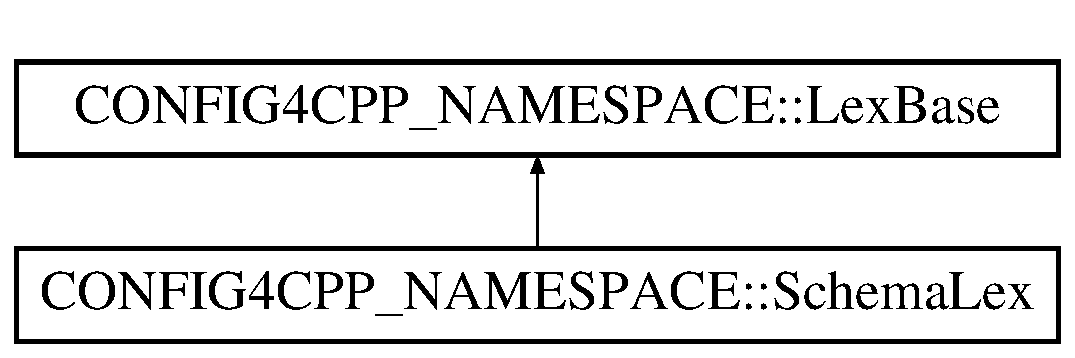
\includegraphics[height=2.000000cm]{classCONFIG4CPP__NAMESPACE_1_1SchemaLex}
\end{center}
\end{figure}
\subsection*{Public Types}
\begin{DoxyCompactItemize}
\item 
enum {\bfseries Schema\-Lex\-Symbols} \{ \\*
{\bfseries L\-E\-X\-\_\-\-I\-G\-N\-O\-R\-E\-\_\-\-E\-V\-E\-R\-Y\-T\-H\-I\-N\-G\-\_\-\-I\-N\-\_\-\-S\-Y\-M} = 101, 
{\bfseries L\-E\-X\-\_\-\-I\-G\-N\-O\-R\-E\-\_\-\-S\-C\-O\-P\-E\-S\-\_\-\-I\-N\-\_\-\-S\-Y\-M} = 102, 
{\bfseries L\-E\-X\-\_\-\-I\-G\-N\-O\-R\-E\-\_\-\-V\-A\-R\-I\-A\-B\-L\-E\-S\-\_\-\-I\-N\-\_\-\-S\-Y\-M} = 103, 
{\bfseries L\-E\-X\-\_\-\-T\-Y\-P\-E\-D\-E\-F\-\_\-\-S\-Y\-M} = 104, 
\\*
{\bfseries L\-E\-X\-\_\-\-O\-P\-T\-I\-O\-N\-A\-L\-\_\-\-S\-Y\-M} = 105, 
{\bfseries L\-E\-X\-\_\-\-R\-E\-Q\-U\-I\-R\-E\-D\-\_\-\-S\-Y\-M} = 106
 \}
\end{DoxyCompactItemize}
\subsection*{Public Member Functions}
\begin{DoxyCompactItemize}
\item 
\hypertarget{classCONFIG4CPP__NAMESPACE_1_1SchemaLex_a1f2d21646bc92a783f2fd29e6f2652e8}{{\bfseries Schema\-Lex} (const char $\ast$str)  throw (\-Configuration\-Exception)}\label{classCONFIG4CPP__NAMESPACE_1_1SchemaLex_a1f2d21646bc92a783f2fd29e6f2652e8}

\end{DoxyCompactItemize}
\subsection*{Additional Inherited Members}


The documentation for this class was generated from the following files\-:\begin{DoxyCompactItemize}
\item 
src/configuration/config4cpp/src/Schema\-Lex.\-h\item 
src/configuration/config4cpp/src/Schema\-Lex.\-cpp\end{DoxyCompactItemize}

\hypertarget{classCONFIG4CPP__NAMESPACE_1_1SchemaParser}{\section{C\-O\-N\-F\-I\-G4\-C\-P\-P\-\_\-\-N\-A\-M\-E\-S\-P\-A\-C\-E\-:\-:Schema\-Parser Class Reference}
\label{classCONFIG4CPP__NAMESPACE_1_1SchemaParser}\index{C\-O\-N\-F\-I\-G4\-C\-P\-P\-\_\-\-N\-A\-M\-E\-S\-P\-A\-C\-E\-::\-Schema\-Parser@{C\-O\-N\-F\-I\-G4\-C\-P\-P\-\_\-\-N\-A\-M\-E\-S\-P\-A\-C\-E\-::\-Schema\-Parser}}
}
\subsection*{Public Member Functions}
\begin{DoxyCompactItemize}
\item 
\hypertarget{classCONFIG4CPP__NAMESPACE_1_1SchemaParser_a0ea76efcbf6e58cd6adc32011ac973a9}{{\bfseries Schema\-Parser} (\hyperlink{classCONFIG4CPP__NAMESPACE_1_1SchemaValidator}{Schema\-Validator} $\ast$sv)}\label{classCONFIG4CPP__NAMESPACE_1_1SchemaParser_a0ea76efcbf6e58cd6adc32011ac973a9}

\item 
\hypertarget{classCONFIG4CPP__NAMESPACE_1_1SchemaParser_ae6931178354fc66e3d4a977d43d43a68}{void {\bfseries parse} (const char $\ast$$\ast$schema, int schema\-Size)  throw (\-Configuration\-Exception)}\label{classCONFIG4CPP__NAMESPACE_1_1SchemaParser_ae6931178354fc66e3d4a977d43d43a68}

\end{DoxyCompactItemize}


The documentation for this class was generated from the following files\-:\begin{DoxyCompactItemize}
\item 
src/configuration/config4cpp/src/Schema\-Parser.\-h\item 
src/configuration/config4cpp/src/Schema\-Parser.\-cpp\end{DoxyCompactItemize}

\hypertarget{classCONFIG4CPP__NAMESPACE_1_1SchemaType}{\section{C\-O\-N\-F\-I\-G4\-C\-P\-P\-\_\-\-N\-A\-M\-E\-S\-P\-A\-C\-E\-:\-:Schema\-Type Class Reference}
\label{classCONFIG4CPP__NAMESPACE_1_1SchemaType}\index{C\-O\-N\-F\-I\-G4\-C\-P\-P\-\_\-\-N\-A\-M\-E\-S\-P\-A\-C\-E\-::\-Schema\-Type@{C\-O\-N\-F\-I\-G4\-C\-P\-P\-\_\-\-N\-A\-M\-E\-S\-P\-A\-C\-E\-::\-Schema\-Type}}
}
Inheritance diagram for C\-O\-N\-F\-I\-G4\-C\-P\-P\-\_\-\-N\-A\-M\-E\-S\-P\-A\-C\-E\-:\-:Schema\-Type\-:\begin{figure}[H]
\begin{center}
\leavevmode
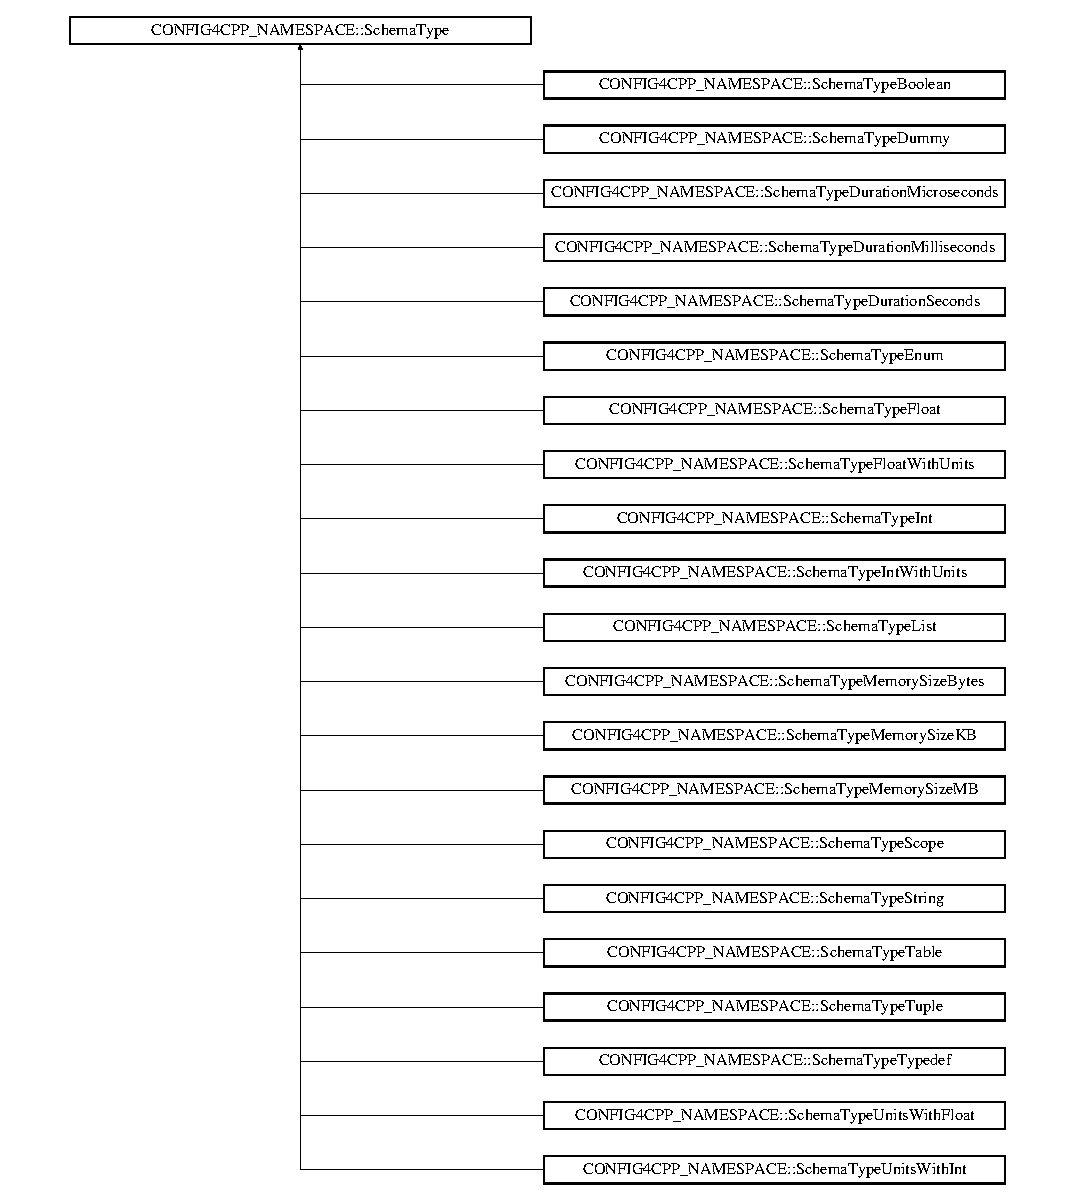
\includegraphics[height=12.000000cm]{classCONFIG4CPP__NAMESPACE_1_1SchemaType}
\end{center}
\end{figure}
\subsection*{Public Member Functions}
\begin{DoxyCompactItemize}
\item 
\hypertarget{classCONFIG4CPP__NAMESPACE_1_1SchemaType_a253d19cc29fbc5c77cdacff617b155a4}{{\bfseries Schema\-Type} (const char $\ast$type\-Name, const char $\ast$class\-Name, Configuration\-::\-Type cfg\-Type)}\label{classCONFIG4CPP__NAMESPACE_1_1SchemaType_a253d19cc29fbc5c77cdacff617b155a4}

\item 
\hypertarget{classCONFIG4CPP__NAMESPACE_1_1SchemaType_acee6e27a98ec3b847e9b7ed52d7bdfc5}{const char $\ast$ {\bfseries type\-Name} () const }\label{classCONFIG4CPP__NAMESPACE_1_1SchemaType_acee6e27a98ec3b847e9b7ed52d7bdfc5}

\item 
\hypertarget{classCONFIG4CPP__NAMESPACE_1_1SchemaType_a9db17b690f59eae1b9e56d731db7350f}{const char $\ast$ {\bfseries class\-Name} () const }\label{classCONFIG4CPP__NAMESPACE_1_1SchemaType_a9db17b690f59eae1b9e56d731db7350f}

\item 
\hypertarget{classCONFIG4CPP__NAMESPACE_1_1SchemaType_a996bbaa17ce3ca52951b7a64977b1ac7}{Configuration\-::\-Type {\bfseries cfg\-Type} () const }\label{classCONFIG4CPP__NAMESPACE_1_1SchemaType_a996bbaa17ce3ca52951b7a64977b1ac7}

\end{DoxyCompactItemize}
\subsection*{Protected Member Functions}
\begin{DoxyCompactItemize}
\item 
\hypertarget{classCONFIG4CPP__NAMESPACE_1_1SchemaType_a7951ab8f525833bc06272820f69733ea}{virtual void {\bfseries check\-Rule} (const \hyperlink{classCONFIG4CPP__NAMESPACE_1_1SchemaValidator}{Schema\-Validator} $\ast$sv, const \hyperlink{classCONFIG4CPP__NAMESPACE_1_1Configuration}{Configuration} $\ast$cfg, const char $\ast$type\-Name, const \hyperlink{classCONFIG4CPP__NAMESPACE_1_1StringVector}{String\-Vector} \&type\-Args, const char $\ast$rule) const =0  throw (\-Configuration\-Exception)}\label{classCONFIG4CPP__NAMESPACE_1_1SchemaType_a7951ab8f525833bc06272820f69733ea}

\item 
\hypertarget{classCONFIG4CPP__NAMESPACE_1_1SchemaType_a694211a9a083ac45039dbe888c8ada6e}{virtual void {\bfseries validate} (const \hyperlink{classCONFIG4CPP__NAMESPACE_1_1SchemaValidator}{Schema\-Validator} $\ast$sv, const \hyperlink{classCONFIG4CPP__NAMESPACE_1_1Configuration}{Configuration} $\ast$cfg, const char $\ast$scope, const char $\ast$name, const char $\ast$type\-Name, const char $\ast$orig\-Type\-Name, const \hyperlink{classCONFIG4CPP__NAMESPACE_1_1StringVector}{String\-Vector} \&type\-Args, int indent\-Level) const   throw (\-Configuration\-Exception)}\label{classCONFIG4CPP__NAMESPACE_1_1SchemaType_a694211a9a083ac45039dbe888c8ada6e}

\item 
\hypertarget{classCONFIG4CPP__NAMESPACE_1_1SchemaType_ac2dcd5eb5d90d17f9b24ecd67758f79b}{virtual bool {\bfseries is\-A} (const \hyperlink{classCONFIG4CPP__NAMESPACE_1_1SchemaValidator}{Schema\-Validator} $\ast$sv, const \hyperlink{classCONFIG4CPP__NAMESPACE_1_1Configuration}{Configuration} $\ast$cfg, const char $\ast$value, const char $\ast$type\-Name, const \hyperlink{classCONFIG4CPP__NAMESPACE_1_1StringVector}{String\-Vector} \&type\-Args, int indent\-Level, \hyperlink{classCONFIG4CPP__NAMESPACE_1_1StringBuffer}{String\-Buffer} \&err\-Suffix) const }\label{classCONFIG4CPP__NAMESPACE_1_1SchemaType_ac2dcd5eb5d90d17f9b24ecd67758f79b}

\item 
\hypertarget{classCONFIG4CPP__NAMESPACE_1_1SchemaType_a7417b9c4739c2e02a3df352bdaf52add}{\hyperlink{classCONFIG4CPP__NAMESPACE_1_1SchemaType}{Schema\-Type} $\ast$ {\bfseries find\-Type} (const \hyperlink{classCONFIG4CPP__NAMESPACE_1_1SchemaValidator}{Schema\-Validator} $\ast$sv, const char $\ast$name) const }\label{classCONFIG4CPP__NAMESPACE_1_1SchemaType_a7417b9c4739c2e02a3df352bdaf52add}

\item 
\hypertarget{classCONFIG4CPP__NAMESPACE_1_1SchemaType_a0c6f1eea6ea1f6c84fe013a9b12fa2a7}{void {\bfseries call\-Validate} (const \hyperlink{classCONFIG4CPP__NAMESPACE_1_1SchemaType}{Schema\-Type} $\ast$target, const \hyperlink{classCONFIG4CPP__NAMESPACE_1_1SchemaValidator}{Schema\-Validator} $\ast$sv, const \hyperlink{classCONFIG4CPP__NAMESPACE_1_1Configuration}{Configuration} $\ast$cfg, const char $\ast$scope, const char $\ast$name, const char $\ast$type\-Name, const char $\ast$orig\-Type\-Name, const \hyperlink{classCONFIG4CPP__NAMESPACE_1_1StringVector}{String\-Vector} \&type\-Args, int indent\-Level) const   throw (\-Configuration\-Exception)}\label{classCONFIG4CPP__NAMESPACE_1_1SchemaType_a0c6f1eea6ea1f6c84fe013a9b12fa2a7}

\item 
\hypertarget{classCONFIG4CPP__NAMESPACE_1_1SchemaType_a83f255330f3ae79110adbccf9e6ecc06}{bool {\bfseries call\-Is\-A} (const \hyperlink{classCONFIG4CPP__NAMESPACE_1_1SchemaType}{Schema\-Type} $\ast$target, const \hyperlink{classCONFIG4CPP__NAMESPACE_1_1SchemaValidator}{Schema\-Validator} $\ast$sv, const \hyperlink{classCONFIG4CPP__NAMESPACE_1_1Configuration}{Configuration} $\ast$cfg, const char $\ast$value, const char $\ast$type\-Name, const \hyperlink{classCONFIG4CPP__NAMESPACE_1_1StringVector}{String\-Vector} \&type\-Args, int indent\-Level, \hyperlink{classCONFIG4CPP__NAMESPACE_1_1StringBuffer}{String\-Buffer} \&err\-Suffix) const }\label{classCONFIG4CPP__NAMESPACE_1_1SchemaType_a83f255330f3ae79110adbccf9e6ecc06}

\end{DoxyCompactItemize}
\subsection*{Friends}
\begin{DoxyCompactItemize}
\item 
\hypertarget{classCONFIG4CPP__NAMESPACE_1_1SchemaType_af8cde46b6af04882af19fea29321f27b}{class {\bfseries Schema\-Validator}}\label{classCONFIG4CPP__NAMESPACE_1_1SchemaType_af8cde46b6af04882af19fea29321f27b}

\item 
\hypertarget{classCONFIG4CPP__NAMESPACE_1_1SchemaType_aacf417b319ed18d9192f294e9267b3b7}{class {\bfseries Schema\-Parser}}\label{classCONFIG4CPP__NAMESPACE_1_1SchemaType_aacf417b319ed18d9192f294e9267b3b7}

\end{DoxyCompactItemize}


The documentation for this class was generated from the following files\-:\begin{DoxyCompactItemize}
\item 
src/configuration/config4cpp/include/config4cpp/Schema\-Type.\-h\item 
src/configuration/config4cpp/src/Schema\-Type.\-cpp\end{DoxyCompactItemize}

\hypertarget{classCONFIG4CPP__NAMESPACE_1_1SchemaTypeBoolean}{\section{C\-O\-N\-F\-I\-G4\-C\-P\-P\-\_\-\-N\-A\-M\-E\-S\-P\-A\-C\-E\-:\-:Schema\-Type\-Boolean Class Reference}
\label{classCONFIG4CPP__NAMESPACE_1_1SchemaTypeBoolean}\index{C\-O\-N\-F\-I\-G4\-C\-P\-P\-\_\-\-N\-A\-M\-E\-S\-P\-A\-C\-E\-::\-Schema\-Type\-Boolean@{C\-O\-N\-F\-I\-G4\-C\-P\-P\-\_\-\-N\-A\-M\-E\-S\-P\-A\-C\-E\-::\-Schema\-Type\-Boolean}}
}
Inheritance diagram for C\-O\-N\-F\-I\-G4\-C\-P\-P\-\_\-\-N\-A\-M\-E\-S\-P\-A\-C\-E\-:\-:Schema\-Type\-Boolean\-:\begin{figure}[H]
\begin{center}
\leavevmode
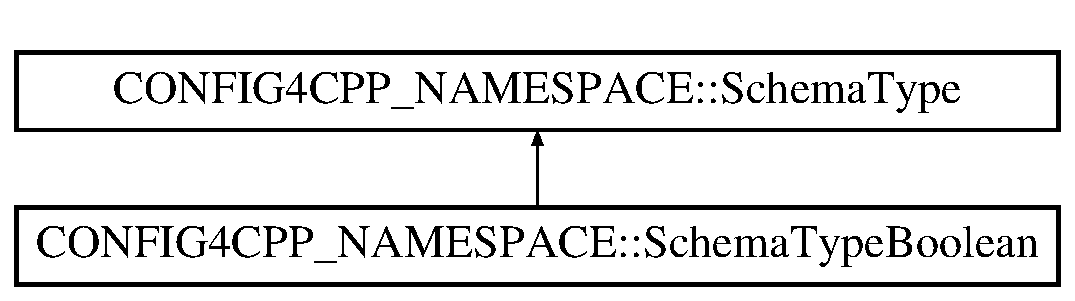
\includegraphics[height=2.000000cm]{classCONFIG4CPP__NAMESPACE_1_1SchemaTypeBoolean}
\end{center}
\end{figure}
\subsection*{Protected Member Functions}
\begin{DoxyCompactItemize}
\item 
\hypertarget{classCONFIG4CPP__NAMESPACE_1_1SchemaTypeBoolean_aec05deaa9bedbafd61ca2dc70de28f89}{virtual void {\bfseries check\-Rule} (const \hyperlink{classCONFIG4CPP__NAMESPACE_1_1SchemaValidator}{Schema\-Validator} $\ast$sv, const \hyperlink{classCONFIG4CPP__NAMESPACE_1_1Configuration}{Configuration} $\ast$cfg, const char $\ast$type\-Name, const \hyperlink{classCONFIG4CPP__NAMESPACE_1_1StringVector}{String\-Vector} \&type\-Args, const char $\ast$rule) const   throw (\-Configuration\-Exception)}\label{classCONFIG4CPP__NAMESPACE_1_1SchemaTypeBoolean_aec05deaa9bedbafd61ca2dc70de28f89}

\item 
\hypertarget{classCONFIG4CPP__NAMESPACE_1_1SchemaTypeBoolean_ac3a38510bba85c292425eaf65934d542}{virtual bool {\bfseries is\-A} (const \hyperlink{classCONFIG4CPP__NAMESPACE_1_1SchemaValidator}{Schema\-Validator} $\ast$sv, const \hyperlink{classCONFIG4CPP__NAMESPACE_1_1Configuration}{Configuration} $\ast$cfg, const char $\ast$value, const char $\ast$type\-Name, const \hyperlink{classCONFIG4CPP__NAMESPACE_1_1StringVector}{String\-Vector} \&type\-Args, int indent\-Level, \hyperlink{classCONFIG4CPP__NAMESPACE_1_1StringBuffer}{String\-Buffer} \&err\-Suffix) const }\label{classCONFIG4CPP__NAMESPACE_1_1SchemaTypeBoolean_ac3a38510bba85c292425eaf65934d542}

\end{DoxyCompactItemize}
\subsection*{Additional Inherited Members}


The documentation for this class was generated from the following files\-:\begin{DoxyCompactItemize}
\item 
src/configuration/config4cpp/src/Schema\-Type\-Boolean.\-h\item 
src/configuration/config4cpp/src/Schema\-Type\-Boolean.\-cpp\end{DoxyCompactItemize}

\hypertarget{classCONFIG4CPP__NAMESPACE_1_1SchemaTypeDummy}{\section{C\-O\-N\-F\-I\-G4\-C\-P\-P\-\_\-\-N\-A\-M\-E\-S\-P\-A\-C\-E\-:\-:Schema\-Type\-Dummy Class Reference}
\label{classCONFIG4CPP__NAMESPACE_1_1SchemaTypeDummy}\index{C\-O\-N\-F\-I\-G4\-C\-P\-P\-\_\-\-N\-A\-M\-E\-S\-P\-A\-C\-E\-::\-Schema\-Type\-Dummy@{C\-O\-N\-F\-I\-G4\-C\-P\-P\-\_\-\-N\-A\-M\-E\-S\-P\-A\-C\-E\-::\-Schema\-Type\-Dummy}}
}
Inheritance diagram for C\-O\-N\-F\-I\-G4\-C\-P\-P\-\_\-\-N\-A\-M\-E\-S\-P\-A\-C\-E\-:\-:Schema\-Type\-Dummy\-:\begin{figure}[H]
\begin{center}
\leavevmode
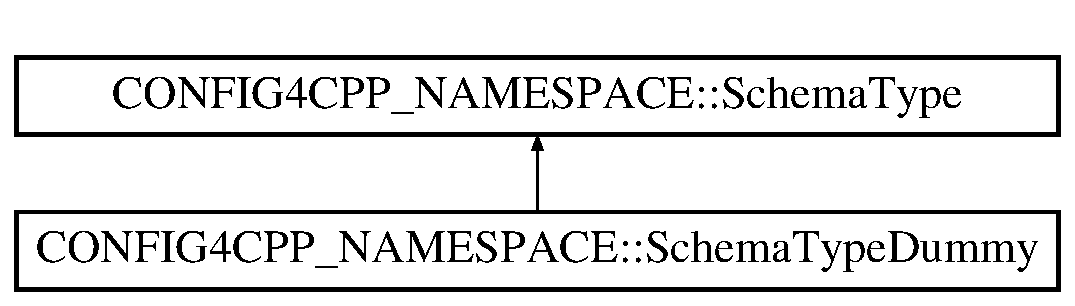
\includegraphics[height=2.000000cm]{classCONFIG4CPP__NAMESPACE_1_1SchemaTypeDummy}
\end{center}
\end{figure}
\subsection*{Public Member Functions}
\begin{DoxyCompactItemize}
\item 
\hypertarget{classCONFIG4CPP__NAMESPACE_1_1SchemaTypeDummy_ab478e0fbf1d8e3364fca9c5ee8bbcc01}{{\bfseries Schema\-Type\-Dummy} (const char $\ast$name)}\label{classCONFIG4CPP__NAMESPACE_1_1SchemaTypeDummy_ab478e0fbf1d8e3364fca9c5ee8bbcc01}

\end{DoxyCompactItemize}
\subsection*{Protected Member Functions}
\begin{DoxyCompactItemize}
\item 
\hypertarget{classCONFIG4CPP__NAMESPACE_1_1SchemaTypeDummy_ae5e027c3a7207a8c197df57631daa2c0}{virtual void {\bfseries check\-Rule} (const \hyperlink{classCONFIG4CPP__NAMESPACE_1_1SchemaValidator}{Schema\-Validator} $\ast$sv, const \hyperlink{classCONFIG4CPP__NAMESPACE_1_1Configuration}{Configuration} $\ast$cfg, const char $\ast$type\-Name, const \hyperlink{classCONFIG4CPP__NAMESPACE_1_1StringVector}{String\-Vector} \&type\-Args, const char $\ast$rule) const   throw (\-Configuration\-Exception)}\label{classCONFIG4CPP__NAMESPACE_1_1SchemaTypeDummy_ae5e027c3a7207a8c197df57631daa2c0}

\end{DoxyCompactItemize}


The documentation for this class was generated from the following file\-:\begin{DoxyCompactItemize}
\item 
src/configuration/config4cpp/src/Schema\-Type\-Dummy.\-h\end{DoxyCompactItemize}

\hypertarget{classCONFIG4CPP__NAMESPACE_1_1SchemaTypeDurationMicroseconds}{\section{C\-O\-N\-F\-I\-G4\-C\-P\-P\-\_\-\-N\-A\-M\-E\-S\-P\-A\-C\-E\-:\-:Schema\-Type\-Duration\-Microseconds Class Reference}
\label{classCONFIG4CPP__NAMESPACE_1_1SchemaTypeDurationMicroseconds}\index{C\-O\-N\-F\-I\-G4\-C\-P\-P\-\_\-\-N\-A\-M\-E\-S\-P\-A\-C\-E\-::\-Schema\-Type\-Duration\-Microseconds@{C\-O\-N\-F\-I\-G4\-C\-P\-P\-\_\-\-N\-A\-M\-E\-S\-P\-A\-C\-E\-::\-Schema\-Type\-Duration\-Microseconds}}
}
Inheritance diagram for C\-O\-N\-F\-I\-G4\-C\-P\-P\-\_\-\-N\-A\-M\-E\-S\-P\-A\-C\-E\-:\-:Schema\-Type\-Duration\-Microseconds\-:\begin{figure}[H]
\begin{center}
\leavevmode
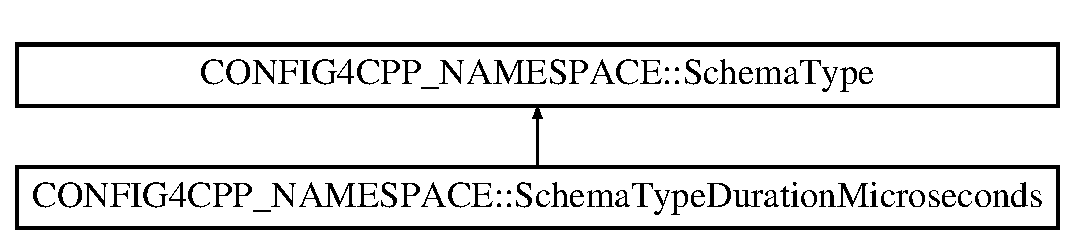
\includegraphics[height=2.000000cm]{classCONFIG4CPP__NAMESPACE_1_1SchemaTypeDurationMicroseconds}
\end{center}
\end{figure}
\subsection*{Protected Member Functions}
\begin{DoxyCompactItemize}
\item 
\hypertarget{classCONFIG4CPP__NAMESPACE_1_1SchemaTypeDurationMicroseconds_afc80af804df0e513e35ef1fd2c037c43}{virtual void {\bfseries check\-Rule} (const \hyperlink{classCONFIG4CPP__NAMESPACE_1_1SchemaValidator}{Schema\-Validator} $\ast$sv, const \hyperlink{classCONFIG4CPP__NAMESPACE_1_1Configuration}{Configuration} $\ast$cfg, const char $\ast$type\-Name, const \hyperlink{classCONFIG4CPP__NAMESPACE_1_1StringVector}{String\-Vector} \&type\-Args, const char $\ast$rule) const   throw (\-Configuration\-Exception)}\label{classCONFIG4CPP__NAMESPACE_1_1SchemaTypeDurationMicroseconds_afc80af804df0e513e35ef1fd2c037c43}

\item 
\hypertarget{classCONFIG4CPP__NAMESPACE_1_1SchemaTypeDurationMicroseconds_a69e256bfce1da5514deb95fc2d3c359e}{virtual bool {\bfseries is\-A} (const \hyperlink{classCONFIG4CPP__NAMESPACE_1_1SchemaValidator}{Schema\-Validator} $\ast$sv, const \hyperlink{classCONFIG4CPP__NAMESPACE_1_1Configuration}{Configuration} $\ast$cfg, const char $\ast$value, const char $\ast$type\-Name, const \hyperlink{classCONFIG4CPP__NAMESPACE_1_1StringVector}{String\-Vector} \&type\-Args, int indent\-Level, \hyperlink{classCONFIG4CPP__NAMESPACE_1_1StringBuffer}{String\-Buffer} \&err\-Suffix) const }\label{classCONFIG4CPP__NAMESPACE_1_1SchemaTypeDurationMicroseconds_a69e256bfce1da5514deb95fc2d3c359e}

\end{DoxyCompactItemize}
\subsection*{Additional Inherited Members}


The documentation for this class was generated from the following files\-:\begin{DoxyCompactItemize}
\item 
src/configuration/config4cpp/src/Schema\-Type\-Duration\-Microseconds.\-h\item 
src/configuration/config4cpp/src/Schema\-Type\-Duration\-Microseconds.\-cpp\end{DoxyCompactItemize}

\hypertarget{classCONFIG4CPP__NAMESPACE_1_1SchemaTypeDurationMilliseconds}{\section{C\-O\-N\-F\-I\-G4\-C\-P\-P\-\_\-\-N\-A\-M\-E\-S\-P\-A\-C\-E\-:\-:Schema\-Type\-Duration\-Milliseconds Class Reference}
\label{classCONFIG4CPP__NAMESPACE_1_1SchemaTypeDurationMilliseconds}\index{C\-O\-N\-F\-I\-G4\-C\-P\-P\-\_\-\-N\-A\-M\-E\-S\-P\-A\-C\-E\-::\-Schema\-Type\-Duration\-Milliseconds@{C\-O\-N\-F\-I\-G4\-C\-P\-P\-\_\-\-N\-A\-M\-E\-S\-P\-A\-C\-E\-::\-Schema\-Type\-Duration\-Milliseconds}}
}
Inheritance diagram for C\-O\-N\-F\-I\-G4\-C\-P\-P\-\_\-\-N\-A\-M\-E\-S\-P\-A\-C\-E\-:\-:Schema\-Type\-Duration\-Milliseconds\-:\begin{figure}[H]
\begin{center}
\leavevmode
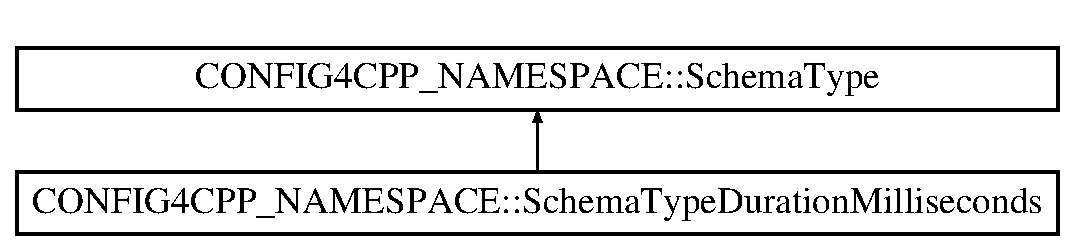
\includegraphics[height=2.000000cm]{classCONFIG4CPP__NAMESPACE_1_1SchemaTypeDurationMilliseconds}
\end{center}
\end{figure}
\subsection*{Protected Member Functions}
\begin{DoxyCompactItemize}
\item 
\hypertarget{classCONFIG4CPP__NAMESPACE_1_1SchemaTypeDurationMilliseconds_a5a8e7547cded8a7e6b88293f7638907f}{virtual void {\bfseries check\-Rule} (const \hyperlink{classCONFIG4CPP__NAMESPACE_1_1SchemaValidator}{Schema\-Validator} $\ast$sv, const \hyperlink{classCONFIG4CPP__NAMESPACE_1_1Configuration}{Configuration} $\ast$cfg, const char $\ast$type\-Name, const \hyperlink{classCONFIG4CPP__NAMESPACE_1_1StringVector}{String\-Vector} \&type\-Args, const char $\ast$rule) const   throw (\-Configuration\-Exception)}\label{classCONFIG4CPP__NAMESPACE_1_1SchemaTypeDurationMilliseconds_a5a8e7547cded8a7e6b88293f7638907f}

\item 
\hypertarget{classCONFIG4CPP__NAMESPACE_1_1SchemaTypeDurationMilliseconds_a3734631f1b28c71a15c4368715419749}{virtual bool {\bfseries is\-A} (const \hyperlink{classCONFIG4CPP__NAMESPACE_1_1SchemaValidator}{Schema\-Validator} $\ast$sv, const \hyperlink{classCONFIG4CPP__NAMESPACE_1_1Configuration}{Configuration} $\ast$cfg, const char $\ast$value, const char $\ast$type\-Name, const \hyperlink{classCONFIG4CPP__NAMESPACE_1_1StringVector}{String\-Vector} \&type\-Args, int indent\-Level, \hyperlink{classCONFIG4CPP__NAMESPACE_1_1StringBuffer}{String\-Buffer} \&err\-Suffix) const }\label{classCONFIG4CPP__NAMESPACE_1_1SchemaTypeDurationMilliseconds_a3734631f1b28c71a15c4368715419749}

\end{DoxyCompactItemize}
\subsection*{Additional Inherited Members}


The documentation for this class was generated from the following files\-:\begin{DoxyCompactItemize}
\item 
src/configuration/config4cpp/src/Schema\-Type\-Duration\-Milliseconds.\-h\item 
src/configuration/config4cpp/src/Schema\-Type\-Duration\-Milliseconds.\-cpp\end{DoxyCompactItemize}

\hypertarget{classCONFIG4CPP__NAMESPACE_1_1SchemaTypeDurationSeconds}{\section{C\-O\-N\-F\-I\-G4\-C\-P\-P\-\_\-\-N\-A\-M\-E\-S\-P\-A\-C\-E\-:\-:Schema\-Type\-Duration\-Seconds Class Reference}
\label{classCONFIG4CPP__NAMESPACE_1_1SchemaTypeDurationSeconds}\index{C\-O\-N\-F\-I\-G4\-C\-P\-P\-\_\-\-N\-A\-M\-E\-S\-P\-A\-C\-E\-::\-Schema\-Type\-Duration\-Seconds@{C\-O\-N\-F\-I\-G4\-C\-P\-P\-\_\-\-N\-A\-M\-E\-S\-P\-A\-C\-E\-::\-Schema\-Type\-Duration\-Seconds}}
}
Inheritance diagram for C\-O\-N\-F\-I\-G4\-C\-P\-P\-\_\-\-N\-A\-M\-E\-S\-P\-A\-C\-E\-:\-:Schema\-Type\-Duration\-Seconds\-:\begin{figure}[H]
\begin{center}
\leavevmode
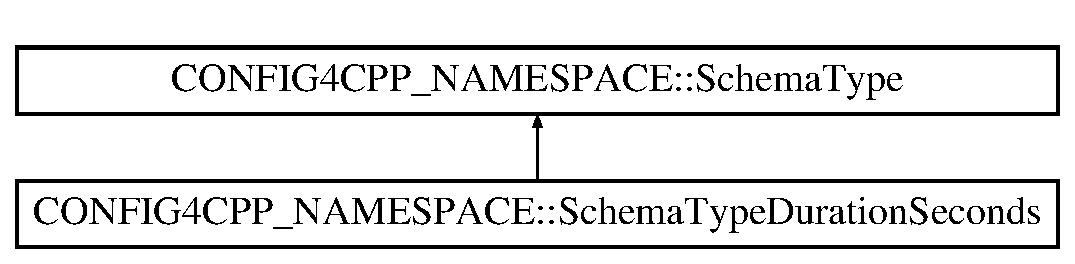
\includegraphics[height=2.000000cm]{classCONFIG4CPP__NAMESPACE_1_1SchemaTypeDurationSeconds}
\end{center}
\end{figure}
\subsection*{Protected Member Functions}
\begin{DoxyCompactItemize}
\item 
\hypertarget{classCONFIG4CPP__NAMESPACE_1_1SchemaTypeDurationSeconds_a510a328ee7f15382c245f517c026231a}{virtual void {\bfseries check\-Rule} (const \hyperlink{classCONFIG4CPP__NAMESPACE_1_1SchemaValidator}{Schema\-Validator} $\ast$sv, const \hyperlink{classCONFIG4CPP__NAMESPACE_1_1Configuration}{Configuration} $\ast$cfg, const char $\ast$type\-Name, const \hyperlink{classCONFIG4CPP__NAMESPACE_1_1StringVector}{String\-Vector} \&type\-Args, const char $\ast$rule) const   throw (\-Configuration\-Exception)}\label{classCONFIG4CPP__NAMESPACE_1_1SchemaTypeDurationSeconds_a510a328ee7f15382c245f517c026231a}

\item 
\hypertarget{classCONFIG4CPP__NAMESPACE_1_1SchemaTypeDurationSeconds_abf008f4905cefc9ab3d537fb3ae6d330}{virtual bool {\bfseries is\-A} (const \hyperlink{classCONFIG4CPP__NAMESPACE_1_1SchemaValidator}{Schema\-Validator} $\ast$sv, const \hyperlink{classCONFIG4CPP__NAMESPACE_1_1Configuration}{Configuration} $\ast$cfg, const char $\ast$value, const char $\ast$type\-Name, const \hyperlink{classCONFIG4CPP__NAMESPACE_1_1StringVector}{String\-Vector} \&type\-Args, int indent\-Level, \hyperlink{classCONFIG4CPP__NAMESPACE_1_1StringBuffer}{String\-Buffer} \&err\-Suffix) const }\label{classCONFIG4CPP__NAMESPACE_1_1SchemaTypeDurationSeconds_abf008f4905cefc9ab3d537fb3ae6d330}

\end{DoxyCompactItemize}
\subsection*{Additional Inherited Members}


The documentation for this class was generated from the following files\-:\begin{DoxyCompactItemize}
\item 
src/configuration/config4cpp/src/Schema\-Type\-Duration\-Seconds.\-h\item 
src/configuration/config4cpp/src/Schema\-Type\-Duration\-Seconds.\-cpp\end{DoxyCompactItemize}

\hypertarget{classCONFIG4CPP__NAMESPACE_1_1SchemaTypeEnum}{\section{C\-O\-N\-F\-I\-G4\-C\-P\-P\-\_\-\-N\-A\-M\-E\-S\-P\-A\-C\-E\-:\-:Schema\-Type\-Enum Class Reference}
\label{classCONFIG4CPP__NAMESPACE_1_1SchemaTypeEnum}\index{C\-O\-N\-F\-I\-G4\-C\-P\-P\-\_\-\-N\-A\-M\-E\-S\-P\-A\-C\-E\-::\-Schema\-Type\-Enum@{C\-O\-N\-F\-I\-G4\-C\-P\-P\-\_\-\-N\-A\-M\-E\-S\-P\-A\-C\-E\-::\-Schema\-Type\-Enum}}
}
Inheritance diagram for C\-O\-N\-F\-I\-G4\-C\-P\-P\-\_\-\-N\-A\-M\-E\-S\-P\-A\-C\-E\-:\-:Schema\-Type\-Enum\-:\begin{figure}[H]
\begin{center}
\leavevmode
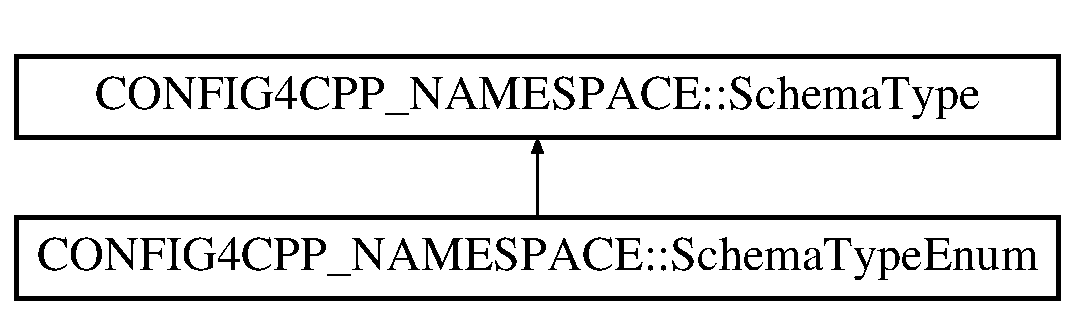
\includegraphics[height=2.000000cm]{classCONFIG4CPP__NAMESPACE_1_1SchemaTypeEnum}
\end{center}
\end{figure}
\subsection*{Protected Member Functions}
\begin{DoxyCompactItemize}
\item 
\hypertarget{classCONFIG4CPP__NAMESPACE_1_1SchemaTypeEnum_aaf382e5d1d332ea0c49086500cfc5f25}{virtual void {\bfseries check\-Rule} (const \hyperlink{classCONFIG4CPP__NAMESPACE_1_1SchemaValidator}{Schema\-Validator} $\ast$sv, const \hyperlink{classCONFIG4CPP__NAMESPACE_1_1Configuration}{Configuration} $\ast$cfg, const char $\ast$type\-Name, const \hyperlink{classCONFIG4CPP__NAMESPACE_1_1StringVector}{String\-Vector} \&type\-Args, const char $\ast$rule) const   throw (\-Configuration\-Exception)}\label{classCONFIG4CPP__NAMESPACE_1_1SchemaTypeEnum_aaf382e5d1d332ea0c49086500cfc5f25}

\item 
\hypertarget{classCONFIG4CPP__NAMESPACE_1_1SchemaTypeEnum_aa8aa23a879e0c82015a4478bca87ee23}{virtual bool {\bfseries is\-A} (const \hyperlink{classCONFIG4CPP__NAMESPACE_1_1SchemaValidator}{Schema\-Validator} $\ast$sv, const \hyperlink{classCONFIG4CPP__NAMESPACE_1_1Configuration}{Configuration} $\ast$cfg, const char $\ast$value, const char $\ast$type\-Name, const \hyperlink{classCONFIG4CPP__NAMESPACE_1_1StringVector}{String\-Vector} \&type\-Args, int indent\-Level, \hyperlink{classCONFIG4CPP__NAMESPACE_1_1StringBuffer}{String\-Buffer} \&err\-Suffix) const }\label{classCONFIG4CPP__NAMESPACE_1_1SchemaTypeEnum_aa8aa23a879e0c82015a4478bca87ee23}

\end{DoxyCompactItemize}
\subsection*{Additional Inherited Members}


The documentation for this class was generated from the following files\-:\begin{DoxyCompactItemize}
\item 
src/configuration/config4cpp/src/Schema\-Type\-Enum.\-h\item 
src/configuration/config4cpp/src/Schema\-Type\-Enum.\-cpp\end{DoxyCompactItemize}

\hypertarget{classCONFIG4CPP__NAMESPACE_1_1SchemaTypeFloat}{\section{C\-O\-N\-F\-I\-G4\-C\-P\-P\-\_\-\-N\-A\-M\-E\-S\-P\-A\-C\-E\-:\-:Schema\-Type\-Float Class Reference}
\label{classCONFIG4CPP__NAMESPACE_1_1SchemaTypeFloat}\index{C\-O\-N\-F\-I\-G4\-C\-P\-P\-\_\-\-N\-A\-M\-E\-S\-P\-A\-C\-E\-::\-Schema\-Type\-Float@{C\-O\-N\-F\-I\-G4\-C\-P\-P\-\_\-\-N\-A\-M\-E\-S\-P\-A\-C\-E\-::\-Schema\-Type\-Float}}
}
Inheritance diagram for C\-O\-N\-F\-I\-G4\-C\-P\-P\-\_\-\-N\-A\-M\-E\-S\-P\-A\-C\-E\-:\-:Schema\-Type\-Float\-:\begin{figure}[H]
\begin{center}
\leavevmode
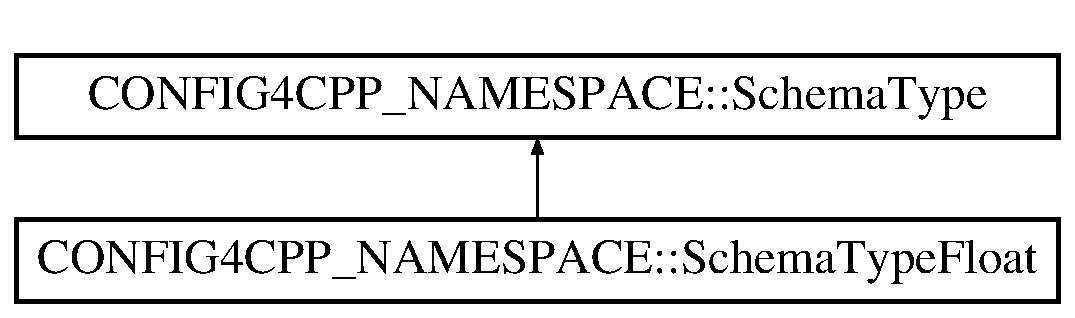
\includegraphics[height=2.000000cm]{classCONFIG4CPP__NAMESPACE_1_1SchemaTypeFloat}
\end{center}
\end{figure}
\subsection*{Protected Member Functions}
\begin{DoxyCompactItemize}
\item 
\hypertarget{classCONFIG4CPP__NAMESPACE_1_1SchemaTypeFloat_a5974a1a853ebae5c77da66f77195e28c}{virtual void {\bfseries check\-Rule} (const \hyperlink{classCONFIG4CPP__NAMESPACE_1_1SchemaValidator}{Schema\-Validator} $\ast$sv, const \hyperlink{classCONFIG4CPP__NAMESPACE_1_1Configuration}{Configuration} $\ast$cfg, const char $\ast$type\-Name, const \hyperlink{classCONFIG4CPP__NAMESPACE_1_1StringVector}{String\-Vector} \&type\-Args, const char $\ast$rule) const   throw (\-Configuration\-Exception)}\label{classCONFIG4CPP__NAMESPACE_1_1SchemaTypeFloat_a5974a1a853ebae5c77da66f77195e28c}

\item 
\hypertarget{classCONFIG4CPP__NAMESPACE_1_1SchemaTypeFloat_a94839b7484832df13ae9aaf1aa5f4637}{virtual bool {\bfseries is\-A} (const \hyperlink{classCONFIG4CPP__NAMESPACE_1_1SchemaValidator}{Schema\-Validator} $\ast$sv, const \hyperlink{classCONFIG4CPP__NAMESPACE_1_1Configuration}{Configuration} $\ast$cfg, const char $\ast$value, const char $\ast$type\-Name, const \hyperlink{classCONFIG4CPP__NAMESPACE_1_1StringVector}{String\-Vector} \&type\-Args, int indent\-Level, \hyperlink{classCONFIG4CPP__NAMESPACE_1_1StringBuffer}{String\-Buffer} \&err\-Suffix) const }\label{classCONFIG4CPP__NAMESPACE_1_1SchemaTypeFloat_a94839b7484832df13ae9aaf1aa5f4637}

\end{DoxyCompactItemize}
\subsection*{Additional Inherited Members}


The documentation for this class was generated from the following files\-:\begin{DoxyCompactItemize}
\item 
src/configuration/config4cpp/src/Schema\-Type\-Float.\-h\item 
src/configuration/config4cpp/src/Schema\-Type\-Float.\-cpp\end{DoxyCompactItemize}

\hypertarget{classCONFIG4CPP__NAMESPACE_1_1SchemaTypeFloatWithUnits}{\section{C\-O\-N\-F\-I\-G4\-C\-P\-P\-\_\-\-N\-A\-M\-E\-S\-P\-A\-C\-E\-:\-:Schema\-Type\-Float\-With\-Units Class Reference}
\label{classCONFIG4CPP__NAMESPACE_1_1SchemaTypeFloatWithUnits}\index{C\-O\-N\-F\-I\-G4\-C\-P\-P\-\_\-\-N\-A\-M\-E\-S\-P\-A\-C\-E\-::\-Schema\-Type\-Float\-With\-Units@{C\-O\-N\-F\-I\-G4\-C\-P\-P\-\_\-\-N\-A\-M\-E\-S\-P\-A\-C\-E\-::\-Schema\-Type\-Float\-With\-Units}}
}
Inheritance diagram for C\-O\-N\-F\-I\-G4\-C\-P\-P\-\_\-\-N\-A\-M\-E\-S\-P\-A\-C\-E\-:\-:Schema\-Type\-Float\-With\-Units\-:\begin{figure}[H]
\begin{center}
\leavevmode
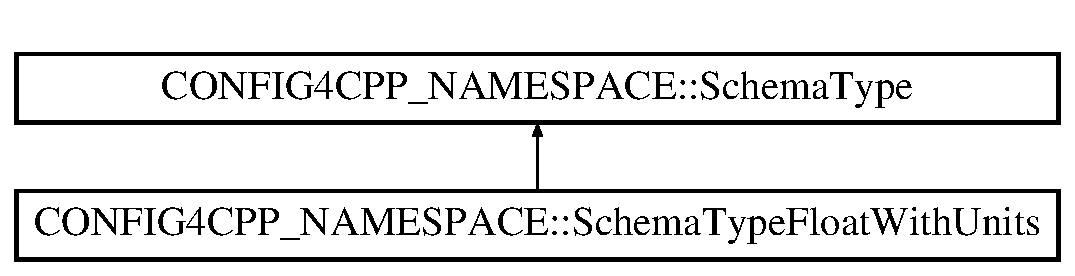
\includegraphics[height=2.000000cm]{classCONFIG4CPP__NAMESPACE_1_1SchemaTypeFloatWithUnits}
\end{center}
\end{figure}
\subsection*{Protected Member Functions}
\begin{DoxyCompactItemize}
\item 
\hypertarget{classCONFIG4CPP__NAMESPACE_1_1SchemaTypeFloatWithUnits_a1ea72ec0463e30c44df4bfdad7823d93}{virtual void {\bfseries check\-Rule} (const \hyperlink{classCONFIG4CPP__NAMESPACE_1_1SchemaValidator}{Schema\-Validator} $\ast$sv, const \hyperlink{classCONFIG4CPP__NAMESPACE_1_1Configuration}{Configuration} $\ast$cfg, const char $\ast$type\-Name, const \hyperlink{classCONFIG4CPP__NAMESPACE_1_1StringVector}{String\-Vector} \&type\-Args, const char $\ast$rule) const   throw (\-Configuration\-Exception)}\label{classCONFIG4CPP__NAMESPACE_1_1SchemaTypeFloatWithUnits_a1ea72ec0463e30c44df4bfdad7823d93}

\item 
\hypertarget{classCONFIG4CPP__NAMESPACE_1_1SchemaTypeFloatWithUnits_a8da15dc6dc03ed0fea6e58f067fcac2c}{virtual bool {\bfseries is\-A} (const \hyperlink{classCONFIG4CPP__NAMESPACE_1_1SchemaValidator}{Schema\-Validator} $\ast$sv, const \hyperlink{classCONFIG4CPP__NAMESPACE_1_1Configuration}{Configuration} $\ast$cfg, const char $\ast$value, const char $\ast$type\-Name, const \hyperlink{classCONFIG4CPP__NAMESPACE_1_1StringVector}{String\-Vector} \&type\-Args, int indent\-Level, \hyperlink{classCONFIG4CPP__NAMESPACE_1_1StringBuffer}{String\-Buffer} \&err\-Suffix) const }\label{classCONFIG4CPP__NAMESPACE_1_1SchemaTypeFloatWithUnits_a8da15dc6dc03ed0fea6e58f067fcac2c}

\end{DoxyCompactItemize}
\subsection*{Additional Inherited Members}


The documentation for this class was generated from the following files\-:\begin{DoxyCompactItemize}
\item 
src/configuration/config4cpp/src/Schema\-Type\-Float\-With\-Units.\-h\item 
src/configuration/config4cpp/src/Schema\-Type\-Float\-With\-Units.\-cpp\end{DoxyCompactItemize}

\hypertarget{classCONFIG4CPP__NAMESPACE_1_1SchemaTypeInt}{\section{C\-O\-N\-F\-I\-G4\-C\-P\-P\-\_\-\-N\-A\-M\-E\-S\-P\-A\-C\-E\-:\-:Schema\-Type\-Int Class Reference}
\label{classCONFIG4CPP__NAMESPACE_1_1SchemaTypeInt}\index{C\-O\-N\-F\-I\-G4\-C\-P\-P\-\_\-\-N\-A\-M\-E\-S\-P\-A\-C\-E\-::\-Schema\-Type\-Int@{C\-O\-N\-F\-I\-G4\-C\-P\-P\-\_\-\-N\-A\-M\-E\-S\-P\-A\-C\-E\-::\-Schema\-Type\-Int}}
}
Inheritance diagram for C\-O\-N\-F\-I\-G4\-C\-P\-P\-\_\-\-N\-A\-M\-E\-S\-P\-A\-C\-E\-:\-:Schema\-Type\-Int\-:\begin{figure}[H]
\begin{center}
\leavevmode
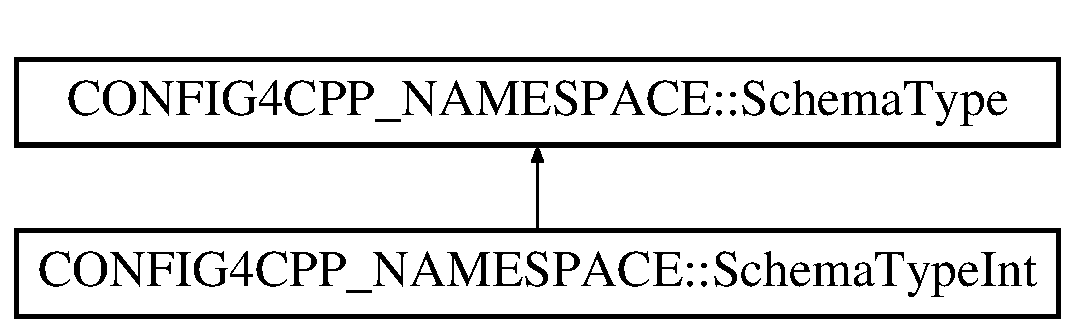
\includegraphics[height=2.000000cm]{classCONFIG4CPP__NAMESPACE_1_1SchemaTypeInt}
\end{center}
\end{figure}
\subsection*{Protected Member Functions}
\begin{DoxyCompactItemize}
\item 
\hypertarget{classCONFIG4CPP__NAMESPACE_1_1SchemaTypeInt_a6ebb03588af3cb8a5ae1c386758a3cad}{virtual void {\bfseries check\-Rule} (const \hyperlink{classCONFIG4CPP__NAMESPACE_1_1SchemaValidator}{Schema\-Validator} $\ast$sv, const \hyperlink{classCONFIG4CPP__NAMESPACE_1_1Configuration}{Configuration} $\ast$cfg, const char $\ast$type\-Name, const \hyperlink{classCONFIG4CPP__NAMESPACE_1_1StringVector}{String\-Vector} \&type\-Args, const char $\ast$rule) const   throw (\-Configuration\-Exception)}\label{classCONFIG4CPP__NAMESPACE_1_1SchemaTypeInt_a6ebb03588af3cb8a5ae1c386758a3cad}

\item 
\hypertarget{classCONFIG4CPP__NAMESPACE_1_1SchemaTypeInt_a04f72619cd3865d6d4a0ac12148f5db0}{virtual bool {\bfseries is\-A} (const \hyperlink{classCONFIG4CPP__NAMESPACE_1_1SchemaValidator}{Schema\-Validator} $\ast$sv, const \hyperlink{classCONFIG4CPP__NAMESPACE_1_1Configuration}{Configuration} $\ast$cfg, const char $\ast$value, const char $\ast$type\-Name, const \hyperlink{classCONFIG4CPP__NAMESPACE_1_1StringVector}{String\-Vector} \&type\-Args, int indent\-Level, \hyperlink{classCONFIG4CPP__NAMESPACE_1_1StringBuffer}{String\-Buffer} \&err\-Suffix) const }\label{classCONFIG4CPP__NAMESPACE_1_1SchemaTypeInt_a04f72619cd3865d6d4a0ac12148f5db0}

\end{DoxyCompactItemize}
\subsection*{Additional Inherited Members}


The documentation for this class was generated from the following files\-:\begin{DoxyCompactItemize}
\item 
src/configuration/config4cpp/src/Schema\-Type\-Int.\-h\item 
src/configuration/config4cpp/src/Schema\-Type\-Int.\-cpp\end{DoxyCompactItemize}

\hypertarget{classCONFIG4CPP__NAMESPACE_1_1SchemaTypeIntWithUnits}{\section{C\-O\-N\-F\-I\-G4\-C\-P\-P\-\_\-\-N\-A\-M\-E\-S\-P\-A\-C\-E\-:\-:Schema\-Type\-Int\-With\-Units Class Reference}
\label{classCONFIG4CPP__NAMESPACE_1_1SchemaTypeIntWithUnits}\index{C\-O\-N\-F\-I\-G4\-C\-P\-P\-\_\-\-N\-A\-M\-E\-S\-P\-A\-C\-E\-::\-Schema\-Type\-Int\-With\-Units@{C\-O\-N\-F\-I\-G4\-C\-P\-P\-\_\-\-N\-A\-M\-E\-S\-P\-A\-C\-E\-::\-Schema\-Type\-Int\-With\-Units}}
}
Inheritance diagram for C\-O\-N\-F\-I\-G4\-C\-P\-P\-\_\-\-N\-A\-M\-E\-S\-P\-A\-C\-E\-:\-:Schema\-Type\-Int\-With\-Units\-:\begin{figure}[H]
\begin{center}
\leavevmode
\includegraphics[height=2.000000cm]{classCONFIG4CPP__NAMESPACE_1_1SchemaTypeIntWithUnits}
\end{center}
\end{figure}
\subsection*{Protected Member Functions}
\begin{DoxyCompactItemize}
\item 
\hypertarget{classCONFIG4CPP__NAMESPACE_1_1SchemaTypeIntWithUnits_ad63ba1b93d1b24f4cb088d8a3fce91bc}{virtual void {\bfseries check\-Rule} (const \hyperlink{classCONFIG4CPP__NAMESPACE_1_1SchemaValidator}{Schema\-Validator} $\ast$sv, const \hyperlink{classCONFIG4CPP__NAMESPACE_1_1Configuration}{Configuration} $\ast$cfg, const char $\ast$type\-Name, const \hyperlink{classCONFIG4CPP__NAMESPACE_1_1StringVector}{String\-Vector} \&type\-Args, const char $\ast$rule) const   throw (\-Configuration\-Exception)}\label{classCONFIG4CPP__NAMESPACE_1_1SchemaTypeIntWithUnits_ad63ba1b93d1b24f4cb088d8a3fce91bc}

\item 
\hypertarget{classCONFIG4CPP__NAMESPACE_1_1SchemaTypeIntWithUnits_a08f3b20ea28fc894b05e290d85721a62}{virtual bool {\bfseries is\-A} (const \hyperlink{classCONFIG4CPP__NAMESPACE_1_1SchemaValidator}{Schema\-Validator} $\ast$sv, const \hyperlink{classCONFIG4CPP__NAMESPACE_1_1Configuration}{Configuration} $\ast$cfg, const char $\ast$value, const char $\ast$type\-Name, const \hyperlink{classCONFIG4CPP__NAMESPACE_1_1StringVector}{String\-Vector} \&type\-Args, int indent\-Level, \hyperlink{classCONFIG4CPP__NAMESPACE_1_1StringBuffer}{String\-Buffer} \&err\-Suffix) const }\label{classCONFIG4CPP__NAMESPACE_1_1SchemaTypeIntWithUnits_a08f3b20ea28fc894b05e290d85721a62}

\end{DoxyCompactItemize}
\subsection*{Additional Inherited Members}


The documentation for this class was generated from the following files\-:\begin{DoxyCompactItemize}
\item 
src/configuration/config4cpp/src/Schema\-Type\-Int\-With\-Units.\-h\item 
src/configuration/config4cpp/src/Schema\-Type\-Int\-With\-Units.\-cpp\end{DoxyCompactItemize}

\hypertarget{classCONFIG4CPP__NAMESPACE_1_1SchemaTypeList}{\section{C\-O\-N\-F\-I\-G4\-C\-P\-P\-\_\-\-N\-A\-M\-E\-S\-P\-A\-C\-E\-:\-:Schema\-Type\-List Class Reference}
\label{classCONFIG4CPP__NAMESPACE_1_1SchemaTypeList}\index{C\-O\-N\-F\-I\-G4\-C\-P\-P\-\_\-\-N\-A\-M\-E\-S\-P\-A\-C\-E\-::\-Schema\-Type\-List@{C\-O\-N\-F\-I\-G4\-C\-P\-P\-\_\-\-N\-A\-M\-E\-S\-P\-A\-C\-E\-::\-Schema\-Type\-List}}
}
Inheritance diagram for C\-O\-N\-F\-I\-G4\-C\-P\-P\-\_\-\-N\-A\-M\-E\-S\-P\-A\-C\-E\-:\-:Schema\-Type\-List\-:\begin{figure}[H]
\begin{center}
\leavevmode
\includegraphics[height=2.000000cm]{classCONFIG4CPP__NAMESPACE_1_1SchemaTypeList}
\end{center}
\end{figure}
\subsection*{Protected Member Functions}
\begin{DoxyCompactItemize}
\item 
\hypertarget{classCONFIG4CPP__NAMESPACE_1_1SchemaTypeList_ab0acf5bb5d7d4313fa79dd19eac29dad}{virtual void {\bfseries check\-Rule} (const \hyperlink{classCONFIG4CPP__NAMESPACE_1_1SchemaValidator}{Schema\-Validator} $\ast$sv, const \hyperlink{classCONFIG4CPP__NAMESPACE_1_1Configuration}{Configuration} $\ast$cfg, const char $\ast$type\-Name, const \hyperlink{classCONFIG4CPP__NAMESPACE_1_1StringVector}{String\-Vector} \&type\-Args, const char $\ast$rule) const   throw (\-Configuration\-Exception)}\label{classCONFIG4CPP__NAMESPACE_1_1SchemaTypeList_ab0acf5bb5d7d4313fa79dd19eac29dad}

\item 
\hypertarget{classCONFIG4CPP__NAMESPACE_1_1SchemaTypeList_aec7f2c63e9bdf39fbcb4a0ee3588229d}{virtual void {\bfseries validate} (const \hyperlink{classCONFIG4CPP__NAMESPACE_1_1SchemaValidator}{Schema\-Validator} $\ast$sv, const \hyperlink{classCONFIG4CPP__NAMESPACE_1_1Configuration}{Configuration} $\ast$cfg, const char $\ast$scope, const char $\ast$name, const char $\ast$type\-Name, const char $\ast$orig\-Type\-Name, const \hyperlink{classCONFIG4CPP__NAMESPACE_1_1StringVector}{String\-Vector} \&type\-Args, int indent\-Level) const   throw (\-Configuration\-Exception)}\label{classCONFIG4CPP__NAMESPACE_1_1SchemaTypeList_aec7f2c63e9bdf39fbcb4a0ee3588229d}

\end{DoxyCompactItemize}
\subsection*{Additional Inherited Members}


The documentation for this class was generated from the following files\-:\begin{DoxyCompactItemize}
\item 
src/configuration/config4cpp/src/Schema\-Type\-List.\-h\item 
src/configuration/config4cpp/src/Schema\-Type\-List.\-cpp\end{DoxyCompactItemize}

\hypertarget{classCONFIG4CPP__NAMESPACE_1_1SchemaTypeMemorySizeBytes}{\section{C\-O\-N\-F\-I\-G4\-C\-P\-P\-\_\-\-N\-A\-M\-E\-S\-P\-A\-C\-E\-:\-:Schema\-Type\-Memory\-Size\-Bytes Class Reference}
\label{classCONFIG4CPP__NAMESPACE_1_1SchemaTypeMemorySizeBytes}\index{C\-O\-N\-F\-I\-G4\-C\-P\-P\-\_\-\-N\-A\-M\-E\-S\-P\-A\-C\-E\-::\-Schema\-Type\-Memory\-Size\-Bytes@{C\-O\-N\-F\-I\-G4\-C\-P\-P\-\_\-\-N\-A\-M\-E\-S\-P\-A\-C\-E\-::\-Schema\-Type\-Memory\-Size\-Bytes}}
}
Inheritance diagram for C\-O\-N\-F\-I\-G4\-C\-P\-P\-\_\-\-N\-A\-M\-E\-S\-P\-A\-C\-E\-:\-:Schema\-Type\-Memory\-Size\-Bytes\-:\begin{figure}[H]
\begin{center}
\leavevmode
\includegraphics[height=2.000000cm]{classCONFIG4CPP__NAMESPACE_1_1SchemaTypeMemorySizeBytes}
\end{center}
\end{figure}
\subsection*{Protected Member Functions}
\begin{DoxyCompactItemize}
\item 
\hypertarget{classCONFIG4CPP__NAMESPACE_1_1SchemaTypeMemorySizeBytes_a3596a3a6c308b6cf2410d10de724945d}{virtual void {\bfseries check\-Rule} (const \hyperlink{classCONFIG4CPP__NAMESPACE_1_1SchemaValidator}{Schema\-Validator} $\ast$sv, const \hyperlink{classCONFIG4CPP__NAMESPACE_1_1Configuration}{Configuration} $\ast$cfg, const char $\ast$type\-Name, const \hyperlink{classCONFIG4CPP__NAMESPACE_1_1StringVector}{String\-Vector} \&type\-Args, const char $\ast$rule) const   throw (\-Configuration\-Exception)}\label{classCONFIG4CPP__NAMESPACE_1_1SchemaTypeMemorySizeBytes_a3596a3a6c308b6cf2410d10de724945d}

\item 
\hypertarget{classCONFIG4CPP__NAMESPACE_1_1SchemaTypeMemorySizeBytes_a8f8e58456b92d82eebc2e627f483df4c}{virtual bool {\bfseries is\-A} (const \hyperlink{classCONFIG4CPP__NAMESPACE_1_1SchemaValidator}{Schema\-Validator} $\ast$sv, const \hyperlink{classCONFIG4CPP__NAMESPACE_1_1Configuration}{Configuration} $\ast$cfg, const char $\ast$value, const char $\ast$type\-Name, const \hyperlink{classCONFIG4CPP__NAMESPACE_1_1StringVector}{String\-Vector} \&type\-Args, int indent\-Level, \hyperlink{classCONFIG4CPP__NAMESPACE_1_1StringBuffer}{String\-Buffer} \&err\-Suffix) const }\label{classCONFIG4CPP__NAMESPACE_1_1SchemaTypeMemorySizeBytes_a8f8e58456b92d82eebc2e627f483df4c}

\end{DoxyCompactItemize}
\subsection*{Additional Inherited Members}


The documentation for this class was generated from the following files\-:\begin{DoxyCompactItemize}
\item 
src/configuration/config4cpp/src/Schema\-Type\-Memory\-Size\-Bytes.\-h\item 
src/configuration/config4cpp/src/Schema\-Type\-Memory\-Size\-Bytes.\-cpp\end{DoxyCompactItemize}

\hypertarget{classCONFIG4CPP__NAMESPACE_1_1SchemaTypeMemorySizeKB}{\section{C\-O\-N\-F\-I\-G4\-C\-P\-P\-\_\-\-N\-A\-M\-E\-S\-P\-A\-C\-E\-:\-:Schema\-Type\-Memory\-Size\-K\-B Class Reference}
\label{classCONFIG4CPP__NAMESPACE_1_1SchemaTypeMemorySizeKB}\index{C\-O\-N\-F\-I\-G4\-C\-P\-P\-\_\-\-N\-A\-M\-E\-S\-P\-A\-C\-E\-::\-Schema\-Type\-Memory\-Size\-K\-B@{C\-O\-N\-F\-I\-G4\-C\-P\-P\-\_\-\-N\-A\-M\-E\-S\-P\-A\-C\-E\-::\-Schema\-Type\-Memory\-Size\-K\-B}}
}
Inheritance diagram for C\-O\-N\-F\-I\-G4\-C\-P\-P\-\_\-\-N\-A\-M\-E\-S\-P\-A\-C\-E\-:\-:Schema\-Type\-Memory\-Size\-K\-B\-:\begin{figure}[H]
\begin{center}
\leavevmode
\includegraphics[height=2.000000cm]{classCONFIG4CPP__NAMESPACE_1_1SchemaTypeMemorySizeKB}
\end{center}
\end{figure}
\subsection*{Protected Member Functions}
\begin{DoxyCompactItemize}
\item 
\hypertarget{classCONFIG4CPP__NAMESPACE_1_1SchemaTypeMemorySizeKB_a7fa93f9f10ae7f5f310a16ad356dfb80}{virtual void {\bfseries check\-Rule} (const \hyperlink{classCONFIG4CPP__NAMESPACE_1_1SchemaValidator}{Schema\-Validator} $\ast$sv, const \hyperlink{classCONFIG4CPP__NAMESPACE_1_1Configuration}{Configuration} $\ast$cfg, const char $\ast$type\-Name, const \hyperlink{classCONFIG4CPP__NAMESPACE_1_1StringVector}{String\-Vector} \&type\-Args, const char $\ast$rule) const   throw (\-Configuration\-Exception)}\label{classCONFIG4CPP__NAMESPACE_1_1SchemaTypeMemorySizeKB_a7fa93f9f10ae7f5f310a16ad356dfb80}

\item 
\hypertarget{classCONFIG4CPP__NAMESPACE_1_1SchemaTypeMemorySizeKB_a9d7f7e5fbdcb7c6c86da243c939d663b}{virtual bool {\bfseries is\-A} (const \hyperlink{classCONFIG4CPP__NAMESPACE_1_1SchemaValidator}{Schema\-Validator} $\ast$sv, const \hyperlink{classCONFIG4CPP__NAMESPACE_1_1Configuration}{Configuration} $\ast$cfg, const char $\ast$value, const char $\ast$type\-Name, const \hyperlink{classCONFIG4CPP__NAMESPACE_1_1StringVector}{String\-Vector} \&type\-Args, int indent\-Level, \hyperlink{classCONFIG4CPP__NAMESPACE_1_1StringBuffer}{String\-Buffer} \&err\-Suffix) const }\label{classCONFIG4CPP__NAMESPACE_1_1SchemaTypeMemorySizeKB_a9d7f7e5fbdcb7c6c86da243c939d663b}

\end{DoxyCompactItemize}
\subsection*{Additional Inherited Members}


The documentation for this class was generated from the following files\-:\begin{DoxyCompactItemize}
\item 
src/configuration/config4cpp/src/Schema\-Type\-Memory\-Size\-K\-B.\-h\item 
src/configuration/config4cpp/src/Schema\-Type\-Memory\-Size\-K\-B.\-cpp\end{DoxyCompactItemize}

\hypertarget{classCONFIG4CPP__NAMESPACE_1_1SchemaTypeMemorySizeMB}{\section{C\-O\-N\-F\-I\-G4\-C\-P\-P\-\_\-\-N\-A\-M\-E\-S\-P\-A\-C\-E\-:\-:Schema\-Type\-Memory\-Size\-M\-B Class Reference}
\label{classCONFIG4CPP__NAMESPACE_1_1SchemaTypeMemorySizeMB}\index{C\-O\-N\-F\-I\-G4\-C\-P\-P\-\_\-\-N\-A\-M\-E\-S\-P\-A\-C\-E\-::\-Schema\-Type\-Memory\-Size\-M\-B@{C\-O\-N\-F\-I\-G4\-C\-P\-P\-\_\-\-N\-A\-M\-E\-S\-P\-A\-C\-E\-::\-Schema\-Type\-Memory\-Size\-M\-B}}
}
Inheritance diagram for C\-O\-N\-F\-I\-G4\-C\-P\-P\-\_\-\-N\-A\-M\-E\-S\-P\-A\-C\-E\-:\-:Schema\-Type\-Memory\-Size\-M\-B\-:\begin{figure}[H]
\begin{center}
\leavevmode
\includegraphics[height=2.000000cm]{classCONFIG4CPP__NAMESPACE_1_1SchemaTypeMemorySizeMB}
\end{center}
\end{figure}
\subsection*{Protected Member Functions}
\begin{DoxyCompactItemize}
\item 
\hypertarget{classCONFIG4CPP__NAMESPACE_1_1SchemaTypeMemorySizeMB_a6f12e23752f296eada46b10ca2ce85d4}{virtual void {\bfseries check\-Rule} (const \hyperlink{classCONFIG4CPP__NAMESPACE_1_1SchemaValidator}{Schema\-Validator} $\ast$sv, const \hyperlink{classCONFIG4CPP__NAMESPACE_1_1Configuration}{Configuration} $\ast$cfg, const char $\ast$type\-Name, const \hyperlink{classCONFIG4CPP__NAMESPACE_1_1StringVector}{String\-Vector} \&type\-Args, const char $\ast$rule) const   throw (\-Configuration\-Exception)}\label{classCONFIG4CPP__NAMESPACE_1_1SchemaTypeMemorySizeMB_a6f12e23752f296eada46b10ca2ce85d4}

\item 
\hypertarget{classCONFIG4CPP__NAMESPACE_1_1SchemaTypeMemorySizeMB_a24e23bc42485480c549bc554f1b40ecf}{virtual bool {\bfseries is\-A} (const \hyperlink{classCONFIG4CPP__NAMESPACE_1_1SchemaValidator}{Schema\-Validator} $\ast$sv, const \hyperlink{classCONFIG4CPP__NAMESPACE_1_1Configuration}{Configuration} $\ast$cfg, const char $\ast$value, const char $\ast$type\-Name, const \hyperlink{classCONFIG4CPP__NAMESPACE_1_1StringVector}{String\-Vector} \&type\-Args, int indent\-Level, \hyperlink{classCONFIG4CPP__NAMESPACE_1_1StringBuffer}{String\-Buffer} \&err\-Suffix) const }\label{classCONFIG4CPP__NAMESPACE_1_1SchemaTypeMemorySizeMB_a24e23bc42485480c549bc554f1b40ecf}

\end{DoxyCompactItemize}
\subsection*{Additional Inherited Members}


The documentation for this class was generated from the following files\-:\begin{DoxyCompactItemize}
\item 
src/configuration/config4cpp/src/Schema\-Type\-Memory\-Size\-M\-B.\-h\item 
src/configuration/config4cpp/src/Schema\-Type\-Memory\-Size\-M\-B.\-cpp\end{DoxyCompactItemize}

\hypertarget{classCONFIG4CPP__NAMESPACE_1_1SchemaTypeScope}{\section{C\-O\-N\-F\-I\-G4\-C\-P\-P\-\_\-\-N\-A\-M\-E\-S\-P\-A\-C\-E\-:\-:Schema\-Type\-Scope Class Reference}
\label{classCONFIG4CPP__NAMESPACE_1_1SchemaTypeScope}\index{C\-O\-N\-F\-I\-G4\-C\-P\-P\-\_\-\-N\-A\-M\-E\-S\-P\-A\-C\-E\-::\-Schema\-Type\-Scope@{C\-O\-N\-F\-I\-G4\-C\-P\-P\-\_\-\-N\-A\-M\-E\-S\-P\-A\-C\-E\-::\-Schema\-Type\-Scope}}
}
Inheritance diagram for C\-O\-N\-F\-I\-G4\-C\-P\-P\-\_\-\-N\-A\-M\-E\-S\-P\-A\-C\-E\-:\-:Schema\-Type\-Scope\-:\begin{figure}[H]
\begin{center}
\leavevmode
\includegraphics[height=2.000000cm]{classCONFIG4CPP__NAMESPACE_1_1SchemaTypeScope}
\end{center}
\end{figure}
\subsection*{Protected Member Functions}
\begin{DoxyCompactItemize}
\item 
\hypertarget{classCONFIG4CPP__NAMESPACE_1_1SchemaTypeScope_af6e7876220705a31af236fa1b483e0e3}{virtual void {\bfseries check\-Rule} (const \hyperlink{classCONFIG4CPP__NAMESPACE_1_1SchemaValidator}{Schema\-Validator} $\ast$sv, const \hyperlink{classCONFIG4CPP__NAMESPACE_1_1Configuration}{Configuration} $\ast$cfg, const char $\ast$type\-Name, const \hyperlink{classCONFIG4CPP__NAMESPACE_1_1StringVector}{String\-Vector} \&type\-Args, const char $\ast$rule) const   throw (\-Configuration\-Exception)}\label{classCONFIG4CPP__NAMESPACE_1_1SchemaTypeScope_af6e7876220705a31af236fa1b483e0e3}

\item 
\hypertarget{classCONFIG4CPP__NAMESPACE_1_1SchemaTypeScope_af41e7e93aabf7a26b225b75e2c10db7f}{virtual void {\bfseries validate} (const \hyperlink{classCONFIG4CPP__NAMESPACE_1_1SchemaValidator}{Schema\-Validator} $\ast$sv, const \hyperlink{classCONFIG4CPP__NAMESPACE_1_1Configuration}{Configuration} $\ast$cfg, const char $\ast$scope, const char $\ast$name, const char $\ast$type\-Name, const char $\ast$orig\-Type\-Name, const \hyperlink{classCONFIG4CPP__NAMESPACE_1_1StringVector}{String\-Vector} \&type\-Args, int indent\-Level) const   throw (\-Configuration\-Exception)}\label{classCONFIG4CPP__NAMESPACE_1_1SchemaTypeScope_af41e7e93aabf7a26b225b75e2c10db7f}

\end{DoxyCompactItemize}
\subsection*{Additional Inherited Members}


The documentation for this class was generated from the following files\-:\begin{DoxyCompactItemize}
\item 
src/configuration/config4cpp/src/Schema\-Type\-Scope.\-h\item 
src/configuration/config4cpp/src/Schema\-Type\-Scope.\-cpp\end{DoxyCompactItemize}

\hypertarget{classCONFIG4CPP__NAMESPACE_1_1SchemaTypeString}{\section{C\-O\-N\-F\-I\-G4\-C\-P\-P\-\_\-\-N\-A\-M\-E\-S\-P\-A\-C\-E\-:\-:Schema\-Type\-String Class Reference}
\label{classCONFIG4CPP__NAMESPACE_1_1SchemaTypeString}\index{C\-O\-N\-F\-I\-G4\-C\-P\-P\-\_\-\-N\-A\-M\-E\-S\-P\-A\-C\-E\-::\-Schema\-Type\-String@{C\-O\-N\-F\-I\-G4\-C\-P\-P\-\_\-\-N\-A\-M\-E\-S\-P\-A\-C\-E\-::\-Schema\-Type\-String}}
}
Inheritance diagram for C\-O\-N\-F\-I\-G4\-C\-P\-P\-\_\-\-N\-A\-M\-E\-S\-P\-A\-C\-E\-:\-:Schema\-Type\-String\-:\begin{figure}[H]
\begin{center}
\leavevmode
\includegraphics[height=2.000000cm]{classCONFIG4CPP__NAMESPACE_1_1SchemaTypeString}
\end{center}
\end{figure}
\subsection*{Protected Member Functions}
\begin{DoxyCompactItemize}
\item 
\hypertarget{classCONFIG4CPP__NAMESPACE_1_1SchemaTypeString_a0ff283e73f950e39dccc14e8ac993fb2}{virtual void {\bfseries check\-Rule} (const \hyperlink{classCONFIG4CPP__NAMESPACE_1_1SchemaValidator}{Schema\-Validator} $\ast$sv, const \hyperlink{classCONFIG4CPP__NAMESPACE_1_1Configuration}{Configuration} $\ast$cfg, const char $\ast$type\-Name, const \hyperlink{classCONFIG4CPP__NAMESPACE_1_1StringVector}{String\-Vector} \&type\-Args, const char $\ast$rule) const   throw (\-Configuration\-Exception)}\label{classCONFIG4CPP__NAMESPACE_1_1SchemaTypeString_a0ff283e73f950e39dccc14e8ac993fb2}

\item 
\hypertarget{classCONFIG4CPP__NAMESPACE_1_1SchemaTypeString_a46c6de9141b2a017e2d539b073fd5aca}{virtual bool {\bfseries is\-A} (const \hyperlink{classCONFIG4CPP__NAMESPACE_1_1SchemaValidator}{Schema\-Validator} $\ast$sv, const \hyperlink{classCONFIG4CPP__NAMESPACE_1_1Configuration}{Configuration} $\ast$cfg, const char $\ast$value, const char $\ast$type\-Name, const \hyperlink{classCONFIG4CPP__NAMESPACE_1_1StringVector}{String\-Vector} \&type\-Args, int indent\-Level, \hyperlink{classCONFIG4CPP__NAMESPACE_1_1StringBuffer}{String\-Buffer} \&err\-Suffix) const }\label{classCONFIG4CPP__NAMESPACE_1_1SchemaTypeString_a46c6de9141b2a017e2d539b073fd5aca}

\end{DoxyCompactItemize}
\subsection*{Additional Inherited Members}


The documentation for this class was generated from the following files\-:\begin{DoxyCompactItemize}
\item 
src/configuration/config4cpp/src/Schema\-Type\-String.\-h\item 
src/configuration/config4cpp/src/Schema\-Type\-String.\-cpp\end{DoxyCompactItemize}

\hypertarget{classCONFIG4CPP__NAMESPACE_1_1SchemaTypeTable}{\section{C\-O\-N\-F\-I\-G4\-C\-P\-P\-\_\-\-N\-A\-M\-E\-S\-P\-A\-C\-E\-:\-:Schema\-Type\-Table Class Reference}
\label{classCONFIG4CPP__NAMESPACE_1_1SchemaTypeTable}\index{C\-O\-N\-F\-I\-G4\-C\-P\-P\-\_\-\-N\-A\-M\-E\-S\-P\-A\-C\-E\-::\-Schema\-Type\-Table@{C\-O\-N\-F\-I\-G4\-C\-P\-P\-\_\-\-N\-A\-M\-E\-S\-P\-A\-C\-E\-::\-Schema\-Type\-Table}}
}
Inheritance diagram for C\-O\-N\-F\-I\-G4\-C\-P\-P\-\_\-\-N\-A\-M\-E\-S\-P\-A\-C\-E\-:\-:Schema\-Type\-Table\-:\begin{figure}[H]
\begin{center}
\leavevmode
\includegraphics[height=2.000000cm]{classCONFIG4CPP__NAMESPACE_1_1SchemaTypeTable}
\end{center}
\end{figure}
\subsection*{Protected Member Functions}
\begin{DoxyCompactItemize}
\item 
\hypertarget{classCONFIG4CPP__NAMESPACE_1_1SchemaTypeTable_ae744a5ee7f922d5c90b2ddf184f35702}{virtual void {\bfseries check\-Rule} (const \hyperlink{classCONFIG4CPP__NAMESPACE_1_1SchemaValidator}{Schema\-Validator} $\ast$sv, const \hyperlink{classCONFIG4CPP__NAMESPACE_1_1Configuration}{Configuration} $\ast$cfg, const char $\ast$type\-Name, const \hyperlink{classCONFIG4CPP__NAMESPACE_1_1StringVector}{String\-Vector} \&type\-Args, const char $\ast$rule) const   throw (\-Configuration\-Exception)}\label{classCONFIG4CPP__NAMESPACE_1_1SchemaTypeTable_ae744a5ee7f922d5c90b2ddf184f35702}

\item 
\hypertarget{classCONFIG4CPP__NAMESPACE_1_1SchemaTypeTable_a8dddf91ab9ea69358a217da74f0c0b9c}{virtual void {\bfseries validate} (const \hyperlink{classCONFIG4CPP__NAMESPACE_1_1SchemaValidator}{Schema\-Validator} $\ast$sv, const \hyperlink{classCONFIG4CPP__NAMESPACE_1_1Configuration}{Configuration} $\ast$cfg, const char $\ast$scope, const char $\ast$name, const char $\ast$type\-Name, const char $\ast$orig\-Type\-Name, const \hyperlink{classCONFIG4CPP__NAMESPACE_1_1StringVector}{String\-Vector} \&type\-Args, int indent\-Level) const   throw (\-Configuration\-Exception)}\label{classCONFIG4CPP__NAMESPACE_1_1SchemaTypeTable_a8dddf91ab9ea69358a217da74f0c0b9c}

\end{DoxyCompactItemize}
\subsection*{Additional Inherited Members}


The documentation for this class was generated from the following files\-:\begin{DoxyCompactItemize}
\item 
src/configuration/config4cpp/src/Schema\-Type\-Table.\-h\item 
src/configuration/config4cpp/src/Schema\-Type\-Table.\-cpp\end{DoxyCompactItemize}

\hypertarget{classCONFIG4CPP__NAMESPACE_1_1SchemaTypeTuple}{\section{C\-O\-N\-F\-I\-G4\-C\-P\-P\-\_\-\-N\-A\-M\-E\-S\-P\-A\-C\-E\-:\-:Schema\-Type\-Tuple Class Reference}
\label{classCONFIG4CPP__NAMESPACE_1_1SchemaTypeTuple}\index{C\-O\-N\-F\-I\-G4\-C\-P\-P\-\_\-\-N\-A\-M\-E\-S\-P\-A\-C\-E\-::\-Schema\-Type\-Tuple@{C\-O\-N\-F\-I\-G4\-C\-P\-P\-\_\-\-N\-A\-M\-E\-S\-P\-A\-C\-E\-::\-Schema\-Type\-Tuple}}
}
Inheritance diagram for C\-O\-N\-F\-I\-G4\-C\-P\-P\-\_\-\-N\-A\-M\-E\-S\-P\-A\-C\-E\-:\-:Schema\-Type\-Tuple\-:\begin{figure}[H]
\begin{center}
\leavevmode
\includegraphics[height=2.000000cm]{classCONFIG4CPP__NAMESPACE_1_1SchemaTypeTuple}
\end{center}
\end{figure}
\subsection*{Protected Member Functions}
\begin{DoxyCompactItemize}
\item 
\hypertarget{classCONFIG4CPP__NAMESPACE_1_1SchemaTypeTuple_a6bdd97729ffa8cd4319f3d2680ff3dfa}{virtual void {\bfseries check\-Rule} (const \hyperlink{classCONFIG4CPP__NAMESPACE_1_1SchemaValidator}{Schema\-Validator} $\ast$sv, const \hyperlink{classCONFIG4CPP__NAMESPACE_1_1Configuration}{Configuration} $\ast$cfg, const char $\ast$type\-Name, const \hyperlink{classCONFIG4CPP__NAMESPACE_1_1StringVector}{String\-Vector} \&type\-Args, const char $\ast$rule) const   throw (\-Configuration\-Exception)}\label{classCONFIG4CPP__NAMESPACE_1_1SchemaTypeTuple_a6bdd97729ffa8cd4319f3d2680ff3dfa}

\item 
\hypertarget{classCONFIG4CPP__NAMESPACE_1_1SchemaTypeTuple_a0b56e38af19fd1815455ca4db71e48ca}{virtual void {\bfseries validate} (const \hyperlink{classCONFIG4CPP__NAMESPACE_1_1SchemaValidator}{Schema\-Validator} $\ast$sv, const \hyperlink{classCONFIG4CPP__NAMESPACE_1_1Configuration}{Configuration} $\ast$cfg, const char $\ast$scope, const char $\ast$name, const char $\ast$type\-Name, const char $\ast$orig\-Type\-Name, const \hyperlink{classCONFIG4CPP__NAMESPACE_1_1StringVector}{String\-Vector} \&type\-Args, int indent\-Level) const   throw (\-Configuration\-Exception)}\label{classCONFIG4CPP__NAMESPACE_1_1SchemaTypeTuple_a0b56e38af19fd1815455ca4db71e48ca}

\end{DoxyCompactItemize}
\subsection*{Additional Inherited Members}


The documentation for this class was generated from the following files\-:\begin{DoxyCompactItemize}
\item 
src/configuration/config4cpp/src/Schema\-Type\-Tuple.\-h\item 
src/configuration/config4cpp/src/Schema\-Type\-Tuple.\-cpp\end{DoxyCompactItemize}

\hypertarget{classCONFIG4CPP__NAMESPACE_1_1SchemaTypeTypedef}{\section{C\-O\-N\-F\-I\-G4\-C\-P\-P\-\_\-\-N\-A\-M\-E\-S\-P\-A\-C\-E\-:\-:Schema\-Type\-Typedef Class Reference}
\label{classCONFIG4CPP__NAMESPACE_1_1SchemaTypeTypedef}\index{C\-O\-N\-F\-I\-G4\-C\-P\-P\-\_\-\-N\-A\-M\-E\-S\-P\-A\-C\-E\-::\-Schema\-Type\-Typedef@{C\-O\-N\-F\-I\-G4\-C\-P\-P\-\_\-\-N\-A\-M\-E\-S\-P\-A\-C\-E\-::\-Schema\-Type\-Typedef}}
}
Inheritance diagram for C\-O\-N\-F\-I\-G4\-C\-P\-P\-\_\-\-N\-A\-M\-E\-S\-P\-A\-C\-E\-:\-:Schema\-Type\-Typedef\-:\begin{figure}[H]
\begin{center}
\leavevmode
\includegraphics[height=2.000000cm]{classCONFIG4CPP__NAMESPACE_1_1SchemaTypeTypedef}
\end{center}
\end{figure}
\subsection*{Public Member Functions}
\begin{DoxyCompactItemize}
\item 
\hypertarget{classCONFIG4CPP__NAMESPACE_1_1SchemaTypeTypedef_ae8e8cb7914fabf1606b98944588e8efb}{{\bfseries Schema\-Type\-Typedef} (const char $\ast$name, Configuration\-::\-Type cfg\-Type, const char $\ast$base\-Type\-Name, const \hyperlink{classCONFIG4CPP__NAMESPACE_1_1StringVector}{String\-Vector} \&base\-Type\-Args)}\label{classCONFIG4CPP__NAMESPACE_1_1SchemaTypeTypedef_ae8e8cb7914fabf1606b98944588e8efb}

\end{DoxyCompactItemize}
\subsection*{Protected Member Functions}
\begin{DoxyCompactItemize}
\item 
\hypertarget{classCONFIG4CPP__NAMESPACE_1_1SchemaTypeTypedef_af819a0c511863abdb7b92f740c6d1a3c}{virtual void {\bfseries check\-Rule} (const \hyperlink{classCONFIG4CPP__NAMESPACE_1_1SchemaValidator}{Schema\-Validator} $\ast$sv, const \hyperlink{classCONFIG4CPP__NAMESPACE_1_1Configuration}{Configuration} $\ast$cfg, const char $\ast$type\-Name, const \hyperlink{classCONFIG4CPP__NAMESPACE_1_1StringVector}{String\-Vector} \&type\-Args, const char $\ast$rule) const   throw (\-Configuration\-Exception)}\label{classCONFIG4CPP__NAMESPACE_1_1SchemaTypeTypedef_af819a0c511863abdb7b92f740c6d1a3c}

\item 
\hypertarget{classCONFIG4CPP__NAMESPACE_1_1SchemaTypeTypedef_ac4b0d3539b601e4a6189c1267566cd89}{virtual void {\bfseries validate} (const \hyperlink{classCONFIG4CPP__NAMESPACE_1_1SchemaValidator}{Schema\-Validator} $\ast$sv, const \hyperlink{classCONFIG4CPP__NAMESPACE_1_1Configuration}{Configuration} $\ast$cfg, const char $\ast$scope, const char $\ast$name, const char $\ast$type\-Name, const char $\ast$orig\-Type\-Name, const \hyperlink{classCONFIG4CPP__NAMESPACE_1_1StringVector}{String\-Vector} \&type\-Args, int indent\-Level) const   throw (\-Configuration\-Exception)}\label{classCONFIG4CPP__NAMESPACE_1_1SchemaTypeTypedef_ac4b0d3539b601e4a6189c1267566cd89}

\item 
\hypertarget{classCONFIG4CPP__NAMESPACE_1_1SchemaTypeTypedef_a04495ad9037113c17c3add379e4048a0}{virtual bool {\bfseries is\-A} (const \hyperlink{classCONFIG4CPP__NAMESPACE_1_1SchemaValidator}{Schema\-Validator} $\ast$sv, const \hyperlink{classCONFIG4CPP__NAMESPACE_1_1Configuration}{Configuration} $\ast$cfg, const char $\ast$value, const char $\ast$type\-Name, const \hyperlink{classCONFIG4CPP__NAMESPACE_1_1StringVector}{String\-Vector} \&type\-Args, int indent\-Level, \hyperlink{classCONFIG4CPP__NAMESPACE_1_1StringBuffer}{String\-Buffer} \&err\-Suffix) const }\label{classCONFIG4CPP__NAMESPACE_1_1SchemaTypeTypedef_a04495ad9037113c17c3add379e4048a0}

\end{DoxyCompactItemize}


The documentation for this class was generated from the following files\-:\begin{DoxyCompactItemize}
\item 
src/configuration/config4cpp/src/Schema\-Type\-Typedef.\-h\item 
src/configuration/config4cpp/src/Schema\-Type\-Typedef.\-cpp\end{DoxyCompactItemize}

\hypertarget{classCONFIG4CPP__NAMESPACE_1_1SchemaTypeUnitsWithFloat}{\section{C\-O\-N\-F\-I\-G4\-C\-P\-P\-\_\-\-N\-A\-M\-E\-S\-P\-A\-C\-E\-:\-:Schema\-Type\-Units\-With\-Float Class Reference}
\label{classCONFIG4CPP__NAMESPACE_1_1SchemaTypeUnitsWithFloat}\index{C\-O\-N\-F\-I\-G4\-C\-P\-P\-\_\-\-N\-A\-M\-E\-S\-P\-A\-C\-E\-::\-Schema\-Type\-Units\-With\-Float@{C\-O\-N\-F\-I\-G4\-C\-P\-P\-\_\-\-N\-A\-M\-E\-S\-P\-A\-C\-E\-::\-Schema\-Type\-Units\-With\-Float}}
}
Inheritance diagram for C\-O\-N\-F\-I\-G4\-C\-P\-P\-\_\-\-N\-A\-M\-E\-S\-P\-A\-C\-E\-:\-:Schema\-Type\-Units\-With\-Float\-:\begin{figure}[H]
\begin{center}
\leavevmode
\includegraphics[height=2.000000cm]{classCONFIG4CPP__NAMESPACE_1_1SchemaTypeUnitsWithFloat}
\end{center}
\end{figure}
\subsection*{Protected Member Functions}
\begin{DoxyCompactItemize}
\item 
\hypertarget{classCONFIG4CPP__NAMESPACE_1_1SchemaTypeUnitsWithFloat_ab18abdcee0b6ef51fd632137e8894c92}{virtual void {\bfseries check\-Rule} (const \hyperlink{classCONFIG4CPP__NAMESPACE_1_1SchemaValidator}{Schema\-Validator} $\ast$sv, const \hyperlink{classCONFIG4CPP__NAMESPACE_1_1Configuration}{Configuration} $\ast$cfg, const char $\ast$type\-Name, const \hyperlink{classCONFIG4CPP__NAMESPACE_1_1StringVector}{String\-Vector} \&type\-Args, const char $\ast$rule) const   throw (\-Configuration\-Exception)}\label{classCONFIG4CPP__NAMESPACE_1_1SchemaTypeUnitsWithFloat_ab18abdcee0b6ef51fd632137e8894c92}

\item 
\hypertarget{classCONFIG4CPP__NAMESPACE_1_1SchemaTypeUnitsWithFloat_a6de6da017895ddf121714ae797a2df1b}{virtual bool {\bfseries is\-A} (const \hyperlink{classCONFIG4CPP__NAMESPACE_1_1SchemaValidator}{Schema\-Validator} $\ast$sv, const \hyperlink{classCONFIG4CPP__NAMESPACE_1_1Configuration}{Configuration} $\ast$cfg, const char $\ast$value, const char $\ast$type\-Name, const \hyperlink{classCONFIG4CPP__NAMESPACE_1_1StringVector}{String\-Vector} \&type\-Args, int indent\-Level, \hyperlink{classCONFIG4CPP__NAMESPACE_1_1StringBuffer}{String\-Buffer} \&err\-Suffix) const }\label{classCONFIG4CPP__NAMESPACE_1_1SchemaTypeUnitsWithFloat_a6de6da017895ddf121714ae797a2df1b}

\end{DoxyCompactItemize}
\subsection*{Additional Inherited Members}


The documentation for this class was generated from the following files\-:\begin{DoxyCompactItemize}
\item 
src/configuration/config4cpp/src/Schema\-Type\-Units\-With\-Float.\-h\item 
src/configuration/config4cpp/src/Schema\-Type\-Units\-With\-Float.\-cpp\end{DoxyCompactItemize}

\hypertarget{classCONFIG4CPP__NAMESPACE_1_1SchemaTypeUnitsWithInt}{\section{C\-O\-N\-F\-I\-G4\-C\-P\-P\-\_\-\-N\-A\-M\-E\-S\-P\-A\-C\-E\-:\-:Schema\-Type\-Units\-With\-Int Class Reference}
\label{classCONFIG4CPP__NAMESPACE_1_1SchemaTypeUnitsWithInt}\index{C\-O\-N\-F\-I\-G4\-C\-P\-P\-\_\-\-N\-A\-M\-E\-S\-P\-A\-C\-E\-::\-Schema\-Type\-Units\-With\-Int@{C\-O\-N\-F\-I\-G4\-C\-P\-P\-\_\-\-N\-A\-M\-E\-S\-P\-A\-C\-E\-::\-Schema\-Type\-Units\-With\-Int}}
}
Inheritance diagram for C\-O\-N\-F\-I\-G4\-C\-P\-P\-\_\-\-N\-A\-M\-E\-S\-P\-A\-C\-E\-:\-:Schema\-Type\-Units\-With\-Int\-:\begin{figure}[H]
\begin{center}
\leavevmode
\includegraphics[height=2.000000cm]{classCONFIG4CPP__NAMESPACE_1_1SchemaTypeUnitsWithInt}
\end{center}
\end{figure}
\subsection*{Protected Member Functions}
\begin{DoxyCompactItemize}
\item 
\hypertarget{classCONFIG4CPP__NAMESPACE_1_1SchemaTypeUnitsWithInt_a645606fea20bef9951a0a0c542a8e575}{virtual void {\bfseries check\-Rule} (const \hyperlink{classCONFIG4CPP__NAMESPACE_1_1SchemaValidator}{Schema\-Validator} $\ast$sv, const \hyperlink{classCONFIG4CPP__NAMESPACE_1_1Configuration}{Configuration} $\ast$cfg, const char $\ast$type\-Name, const \hyperlink{classCONFIG4CPP__NAMESPACE_1_1StringVector}{String\-Vector} \&type\-Args, const char $\ast$rule) const   throw (\-Configuration\-Exception)}\label{classCONFIG4CPP__NAMESPACE_1_1SchemaTypeUnitsWithInt_a645606fea20bef9951a0a0c542a8e575}

\item 
\hypertarget{classCONFIG4CPP__NAMESPACE_1_1SchemaTypeUnitsWithInt_ae7acc87d36192cefde54c78c8222dacd}{virtual bool {\bfseries is\-A} (const \hyperlink{classCONFIG4CPP__NAMESPACE_1_1SchemaValidator}{Schema\-Validator} $\ast$sv, const \hyperlink{classCONFIG4CPP__NAMESPACE_1_1Configuration}{Configuration} $\ast$cfg, const char $\ast$value, const char $\ast$type\-Name, const \hyperlink{classCONFIG4CPP__NAMESPACE_1_1StringVector}{String\-Vector} \&type\-Args, int indent\-Level, \hyperlink{classCONFIG4CPP__NAMESPACE_1_1StringBuffer}{String\-Buffer} \&err\-Suffix) const }\label{classCONFIG4CPP__NAMESPACE_1_1SchemaTypeUnitsWithInt_ae7acc87d36192cefde54c78c8222dacd}

\end{DoxyCompactItemize}
\subsection*{Additional Inherited Members}


The documentation for this class was generated from the following files\-:\begin{DoxyCompactItemize}
\item 
src/configuration/config4cpp/src/Schema\-Type\-Units\-With\-Int.\-h\item 
src/configuration/config4cpp/src/Schema\-Type\-Units\-With\-Int.\-cpp\end{DoxyCompactItemize}

\hypertarget{classCONFIG4CPP__NAMESPACE_1_1SchemaValidator}{\section{C\-O\-N\-F\-I\-G4\-C\-P\-P\-\_\-\-N\-A\-M\-E\-S\-P\-A\-C\-E\-:\-:Schema\-Validator Class Reference}
\label{classCONFIG4CPP__NAMESPACE_1_1SchemaValidator}\index{C\-O\-N\-F\-I\-G4\-C\-P\-P\-\_\-\-N\-A\-M\-E\-S\-P\-A\-C\-E\-::\-Schema\-Validator@{C\-O\-N\-F\-I\-G4\-C\-P\-P\-\_\-\-N\-A\-M\-E\-S\-P\-A\-C\-E\-::\-Schema\-Validator}}
}
\subsection*{Public Types}
\begin{DoxyCompactItemize}
\item 
enum {\bfseries Force\-Mode} \{ {\bfseries D\-O\-\_\-\-N\-O\-T\-\_\-\-F\-O\-R\-C\-E}, 
{\bfseries F\-O\-R\-C\-E\-\_\-\-O\-P\-T\-I\-O\-N\-A\-L}, 
{\bfseries F\-O\-R\-C\-E\-\_\-\-R\-E\-Q\-U\-I\-R\-E\-D}
 \}
\end{DoxyCompactItemize}
\subsection*{Public Member Functions}
\begin{DoxyCompactItemize}
\item 
\hypertarget{classCONFIG4CPP__NAMESPACE_1_1SchemaValidator_a5dbbf5ecd6ee7969bf5889941084657b}{void {\bfseries want\-Diagnostics} (bool value)}\label{classCONFIG4CPP__NAMESPACE_1_1SchemaValidator_a5dbbf5ecd6ee7969bf5889941084657b}

\item 
\hypertarget{classCONFIG4CPP__NAMESPACE_1_1SchemaValidator_a23e2382ac47e69d12cc44d35e1de4352}{bool {\bfseries want\-Diagnostics} ()}\label{classCONFIG4CPP__NAMESPACE_1_1SchemaValidator_a23e2382ac47e69d12cc44d35e1de4352}

\item 
\hypertarget{classCONFIG4CPP__NAMESPACE_1_1SchemaValidator_a5b75f10c38f46aed325ebe1c222db25d}{void {\bfseries parse\-Schema} (const char $\ast$$\ast$schema, int schema\-Size)  throw (\-Configuration\-Exception)}\label{classCONFIG4CPP__NAMESPACE_1_1SchemaValidator_a5b75f10c38f46aed325ebe1c222db25d}

\item 
\hypertarget{classCONFIG4CPP__NAMESPACE_1_1SchemaValidator_a2eb075c6f649bedaafe38ff6e5c84f2f}{void {\bfseries parse\-Schema} (const char $\ast$$\ast$null\-Terminated\-Schema)  throw (\-Configuration\-Exception)}\label{classCONFIG4CPP__NAMESPACE_1_1SchemaValidator_a2eb075c6f649bedaafe38ff6e5c84f2f}

\item 
\hypertarget{classCONFIG4CPP__NAMESPACE_1_1SchemaValidator_a062b6b1e6444357a647c4e8c4a2e3b77}{void {\bfseries validate} (const \hyperlink{classCONFIG4CPP__NAMESPACE_1_1Configuration}{Configuration} $\ast$cfg, const char $\ast$scope, const char $\ast$local\-Name, Force\-Mode force\-Mode=D\-O\-\_\-\-N\-O\-T\-\_\-\-F\-O\-R\-C\-E) const   throw (\-Configuration\-Exception)}\label{classCONFIG4CPP__NAMESPACE_1_1SchemaValidator_a062b6b1e6444357a647c4e8c4a2e3b77}

\item 
\hypertarget{classCONFIG4CPP__NAMESPACE_1_1SchemaValidator_a1145a4d7ce20fe64ba9c51f8b6322b5b}{void {\bfseries validate} (const \hyperlink{classCONFIG4CPP__NAMESPACE_1_1Configuration}{Configuration} $\ast$cfg, const char $\ast$scope, const char $\ast$local\-Name, bool recurse\-Into\-Subscopes, Configuration\-::\-Type type\-Mask, Force\-Mode force\-Mode=D\-O\-\_\-\-N\-O\-T\-\_\-\-F\-O\-R\-C\-E) const   throw (\-Configuration\-Exception)}\label{classCONFIG4CPP__NAMESPACE_1_1SchemaValidator_a1145a4d7ce20fe64ba9c51f8b6322b5b}

\end{DoxyCompactItemize}
\subsection*{Protected Member Functions}
\begin{DoxyCompactItemize}
\item 
\hypertarget{classCONFIG4CPP__NAMESPACE_1_1SchemaValidator_a0f9a5ec0f1bccf1d6a7ad6683ac79b21}{void {\bfseries register\-Type} (\hyperlink{classCONFIG4CPP__NAMESPACE_1_1SchemaType}{Schema\-Type} $\ast$type)  throw (\-Configuration\-Exception)}\label{classCONFIG4CPP__NAMESPACE_1_1SchemaValidator_a0f9a5ec0f1bccf1d6a7ad6683ac79b21}

\end{DoxyCompactItemize}
\subsection*{Friends}
\begin{DoxyCompactItemize}
\item 
\hypertarget{classCONFIG4CPP__NAMESPACE_1_1SchemaValidator_aacf417b319ed18d9192f294e9267b3b7}{class {\bfseries Schema\-Parser}}\label{classCONFIG4CPP__NAMESPACE_1_1SchemaValidator_aacf417b319ed18d9192f294e9267b3b7}

\item 
\hypertarget{classCONFIG4CPP__NAMESPACE_1_1SchemaValidator_ab2fb09983e4076374aabf2bdf92643ab}{class {\bfseries Schema\-Type}}\label{classCONFIG4CPP__NAMESPACE_1_1SchemaValidator_ab2fb09983e4076374aabf2bdf92643ab}

\item 
\hypertarget{classCONFIG4CPP__NAMESPACE_1_1SchemaValidator_ab71ce25ac9889257c422db208ec91754}{int {\bfseries compare\-Schema\-Id\-Rule\-Info} (const void $\ast$, const void $\ast$)}\label{classCONFIG4CPP__NAMESPACE_1_1SchemaValidator_ab71ce25ac9889257c422db208ec91754}

\item 
\hypertarget{classCONFIG4CPP__NAMESPACE_1_1SchemaValidator_a94d8ea775a97af3b1429081ba297f37d}{int {\bfseries compare\-Schema\-Type} (const void $\ast$, const void $\ast$)}\label{classCONFIG4CPP__NAMESPACE_1_1SchemaValidator_a94d8ea775a97af3b1429081ba297f37d}

\end{DoxyCompactItemize}


The documentation for this class was generated from the following files\-:\begin{DoxyCompactItemize}
\item 
src/configuration/config4cpp/include/config4cpp/Schema\-Validator.\-h\item 
src/configuration/config4cpp/src/Schema\-Validator.\-cpp\end{DoxyCompactItemize}

\hypertarget{classunit_1_1SoundUnit}{}\section{unit\+:\+:Sound\+Unit Class Reference}
\label{classunit_1_1SoundUnit}\index{unit\+::\+Sound\+Unit@{unit\+::\+Sound\+Unit}}


{\ttfamily \#include $<$Sound\+Unit.\+h$>$}

Inheritance diagram for unit\+:\+:Sound\+Unit\+:\begin{figure}[H]
\begin{center}
\leavevmode
\includegraphics[height=3.000000cm]{classunit_1_1SoundUnit}
\end{center}
\end{figure}
\subsection*{Public Member Functions}
\begin{DoxyCompactItemize}
\item 
{\bfseries Sound\+Unit} (std\+::string name)\hypertarget{classunit_1_1SoundUnit_a3220665fe1e433d1b0d90fa328e71133}{}\label{classunit_1_1SoundUnit_a3220665fe1e433d1b0d90fa328e71133}

\item 
void {\bfseries add\+U\+Gen} (\hyperlink{classunit_1_1UGen}{unit\+::\+U\+Gen} $\ast$u)\hypertarget{classunit_1_1SoundUnit_a3c4fb09e94703dd7f7d17ca5cb7bb561}{}\label{classunit_1_1SoundUnit_a3c4fb09e94703dd7f7d17ca5cb7bb561}

\item 
std\+::string {\bfseries get\+Name} ()\hypertarget{classunit_1_1SoundUnit_a4854dfb9b839ff33d061ed013fbf3ef9}{}\label{classunit_1_1SoundUnit_a4854dfb9b839ff33d061ed013fbf3ef9}

\item 
virtual void {\bfseries setup} ()=0\hypertarget{classunit_1_1SoundUnit_aedfa9b99f4555ed5df4ceffe001c1e63}{}\label{classunit_1_1SoundUnit_aedfa9b99f4555ed5df4ceffe001c1e63}

\item 
virtual float {\bfseries tick} ()=0\hypertarget{classunit_1_1SoundUnit_af1f6ccffb8d1919bd774b340c01bea68}{}\label{classunit_1_1SoundUnit_af1f6ccffb8d1919bd774b340c01bea68}

\item 
virtual void {\bfseries process\+Midi\+Message} (int type, int key, float value)=0\hypertarget{classunit_1_1SoundUnit_a1e73f915afac67a2103f8d79daf40ec3}{}\label{classunit_1_1SoundUnit_a1e73f915afac67a2103f8d79daf40ec3}

\item 
virtual void {\bfseries process\+Control\+Message} (int type, int key, float value)=0\hypertarget{classunit_1_1SoundUnit_ad20e07c321b9d206f0f9303bbdf2a67d}{}\label{classunit_1_1SoundUnit_ad20e07c321b9d206f0f9303bbdf2a67d}

\item 
virtual void {\bfseries control} (std\+::string port\+Name, float value)=0\hypertarget{classunit_1_1SoundUnit_a0a74ef3d6c9343f1ee64a9a96bdbbe78}{}\label{classunit_1_1SoundUnit_a0a74ef3d6c9343f1ee64a9a96bdbbe78}

\end{DoxyCompactItemize}
\subsection*{Protected Attributes}
\begin{DoxyCompactItemize}
\item 
std\+::map$<$ std\+::string, \hyperlink{classunit_1_1UGen}{unit\+::\+U\+Gen} $\ast$ $>$ {\bfseries U\+G\+E\+NS}\hypertarget{classunit_1_1SoundUnit_a08f1485a5a06b0d458e99833f9207678}{}\label{classunit_1_1SoundUnit_a08f1485a5a06b0d458e99833f9207678}

\end{DoxyCompactItemize}


\subsection{Detailed Description}
\hyperlink{classunit_1_1SoundUnit}{Sound\+Unit} is an abstract class defining the interface of the sound unit, which represents the concept of a Sound Processing Unit (S\+PU). This S\+PU could be the implementation of a virtual analog synthesizer, a purely digital synthesizer, a digital audio effect or the brand new never heard of sound device you have always dreamt of.

\hyperlink{classunit_1_1SoundUnit}{Sound\+Unit} is derived from \hyperlink{classunit_1_1UGen}{unit\+::\+U\+Gen}, therfore implementations of \hyperlink{classunit_1_1SoundUnit}{Sound\+Unit} can be recursively combined to create more complex \hyperlink{classunit_1_1SoundUnit}{unit\+::\+Sound\+Unit(s)} and \hyperlink{classunit_1_1UGen}{unit\+::\+U\+Gen(s)}.

In an S\+PU you would typically


\begin{DoxyItemize}
\item combine a set of Unit Generators (\hyperlink{classunit_1_1UGen}{unit\+::\+U\+Gen}),
\item define the routing bewtween the U\+Gens
\item define input, output and control ports
\item map the control message to these ports
\end{DoxyItemize}

S\+P\+Us will be registered in \hyperlink{classNeonlicht}{Neonlicht} and incoming Midi and Control messages are then dispatched to the S\+PU. The S\+PU is responsible for processing (or ignoring!) these messages.

Anyway\+: the interface forces you to implement 5 methods\+:


\begin{DoxyItemize}
\item setup() is where you configure and initialize your S\+PU.
\item float tick() is where the actual sound processing takes place
\item process\+Midi\+Message() is where you process the incoming midi data
\item process\+Control\+Message() is where you process the incoming control data
\item control() is where you map messages to internal parameters of the S\+PU
\end{DoxyItemize}

\begin{DoxyAuthor}{Author}
J\+TM 
\end{DoxyAuthor}
\begin{DoxySince}{Since}
April, 2016 
\end{DoxySince}


The documentation for this class was generated from the following files\+:\begin{DoxyCompactItemize}
\item 
unit/Sound\+Unit.\+h\item 
unit/Sound\+Unit.\+cpp\end{DoxyCompactItemize}

\hypertarget{structCONFIG4CPP__NAMESPACE_1_1SpellingAndValue}{\section{C\-O\-N\-F\-I\-G4\-C\-P\-P\-\_\-\-N\-A\-M\-E\-S\-P\-A\-C\-E\-:\-:Spelling\-And\-Value Struct Reference}
\label{structCONFIG4CPP__NAMESPACE_1_1SpellingAndValue}\index{C\-O\-N\-F\-I\-G4\-C\-P\-P\-\_\-\-N\-A\-M\-E\-S\-P\-A\-C\-E\-::\-Spelling\-And\-Value@{C\-O\-N\-F\-I\-G4\-C\-P\-P\-\_\-\-N\-A\-M\-E\-S\-P\-A\-C\-E\-::\-Spelling\-And\-Value}}
}
\subsection*{Public Attributes}
\begin{DoxyCompactItemize}
\item 
\hypertarget{structCONFIG4CPP__NAMESPACE_1_1SpellingAndValue_aefe6e6ddcb5c5241900fe329f8cd615f}{const char $\ast$ {\bfseries spelling}}\label{structCONFIG4CPP__NAMESPACE_1_1SpellingAndValue_aefe6e6ddcb5c5241900fe329f8cd615f}

\item 
\hypertarget{structCONFIG4CPP__NAMESPACE_1_1SpellingAndValue_a2be73af85e1668b820ae7d8747b2d612}{int {\bfseries val}}\label{structCONFIG4CPP__NAMESPACE_1_1SpellingAndValue_a2be73af85e1668b820ae7d8747b2d612}

\end{DoxyCompactItemize}


The documentation for this struct was generated from the following file\-:\begin{DoxyCompactItemize}
\item 
src/configuration/config4cpp/src/Configuration\-Impl.\-h\end{DoxyCompactItemize}

\hypertarget{classunit_1_1SquareGen}{}\section{unit\+:\+:Square\+Gen Class Reference}
\label{classunit_1_1SquareGen}\index{unit\+::\+Square\+Gen@{unit\+::\+Square\+Gen}}
Inheritance diagram for unit\+:\+:Square\+Gen\+:\begin{figure}[H]
\begin{center}
\leavevmode
\includegraphics[height=2.000000cm]{classunit_1_1SquareGen}
\end{center}
\end{figure}
\subsection*{Public Member Functions}
\begin{DoxyCompactItemize}
\item 
{\bfseries Square\+Gen} (std\+::string name)\hypertarget{classunit_1_1SquareGen_a626505e8ade08b9383acda8901aa23b5}{}\label{classunit_1_1SquareGen_a626505e8ade08b9383acda8901aa23b5}

\item 
void {\bfseries control} (std\+::string port\+Name, float value)\hypertarget{classunit_1_1SquareGen_a8a25dc2b8c5d1ec7857e4da7ec96cecc}{}\label{classunit_1_1SquareGen_a8a25dc2b8c5d1ec7857e4da7ec96cecc}

\item 
float {\bfseries tick} ()\hypertarget{classunit_1_1SquareGen_a119ab47582ee5814687b87db6a71644c}{}\label{classunit_1_1SquareGen_a119ab47582ee5814687b87db6a71644c}

\end{DoxyCompactItemize}
\subsection*{Additional Inherited Members}


The documentation for this class was generated from the following files\+:\begin{DoxyCompactItemize}
\item 
unit/Square\+Gen.\+h\item 
unit/Square\+Gen.\+cpp\end{DoxyCompactItemize}

\hypertarget{classunit_1_1STKAdapterGen}{}\section{unit\+:\+:S\+T\+K\+Adapter\+Gen Class Reference}
\label{classunit_1_1STKAdapterGen}\index{unit\+::\+S\+T\+K\+Adapter\+Gen@{unit\+::\+S\+T\+K\+Adapter\+Gen}}


{\ttfamily \#include $<$S\+T\+K\+Adapter\+Gen.\+h$>$}

Inheritance diagram for unit\+:\+:S\+T\+K\+Adapter\+Gen\+:\begin{figure}[H]
\begin{center}
\leavevmode
\includegraphics[height=2.333333cm]{classunit_1_1STKAdapterGen}
\end{center}
\end{figure}
\subsection*{Additional Inherited Members}


\subsection{Detailed Description}
\hyperlink{classunit_1_1STKAdapterGen}{S\+T\+K\+Adapter\+Gen} is an intermediate class and acts as a superclass to a number of S\+TK (Synthesis Tool Kit) functions.

To reduce depencies, the S\+TK functions will be replaced with equivalent \hyperlink{classNeonlicht}{Neonlicht} functions in the future.

\begin{DoxyAuthor}{Author}
jtm, email\+:  \href{mailto:milde@hs-fulda.de}{\tt milde@hs-\/fulda.\+de} 
\end{DoxyAuthor}
\begin{DoxySince}{Since}
04-\/2016 
\end{DoxySince}
\begin{DoxyVersion}{Version}
1.\+0 
\end{DoxyVersion}


The documentation for this class was generated from the following file\+:\begin{DoxyCompactItemize}
\item 
include/S\+T\+K\+Adapter\+Gen.\+h\end{DoxyCompactItemize}

\hypertarget{classunit_1_1STKBiQuadGen}{}\section{unit\+:\+:S\+T\+K\+Bi\+Quad\+Gen Class Reference}
\label{classunit_1_1STKBiQuadGen}\index{unit\+::\+S\+T\+K\+Bi\+Quad\+Gen@{unit\+::\+S\+T\+K\+Bi\+Quad\+Gen}}
Inheritance diagram for unit\+:\+:S\+T\+K\+Bi\+Quad\+Gen\+:\begin{figure}[H]
\begin{center}
\leavevmode
\includegraphics[height=3.000000cm]{classunit_1_1STKBiQuadGen}
\end{center}
\end{figure}
\subsection*{Public Member Functions}
\begin{DoxyCompactItemize}
\item 
void {\bfseries control} (std\+::string port\+Name, float value)\hypertarget{classunit_1_1STKBiQuadGen_afbaea4e23ab453fdeaa0069ddd8002a6}{}\label{classunit_1_1STKBiQuadGen_afbaea4e23ab453fdeaa0069ddd8002a6}

\item 
float {\bfseries tick} ()\hypertarget{classunit_1_1STKBiQuadGen_aeaa64c8ff587d9a9089b4cf3276255b9}{}\label{classunit_1_1STKBiQuadGen_aeaa64c8ff587d9a9089b4cf3276255b9}

\end{DoxyCompactItemize}
\subsection*{Additional Inherited Members}


The documentation for this class was generated from the following files\+:\begin{DoxyCompactItemize}
\item 
include/S\+T\+K\+Bi\+Quad\+Gen.\+h\item 
unit/S\+T\+K\+Bi\+Quad\+Gen.\+cpp\end{DoxyCompactItemize}

\hypertarget{classunit_1_1STKOnePoleGen}{\section{unit\-:\-:S\-T\-K\-One\-Pole\-Gen Class Reference}
\label{classunit_1_1STKOnePoleGen}\index{unit\-::\-S\-T\-K\-One\-Pole\-Gen@{unit\-::\-S\-T\-K\-One\-Pole\-Gen}}
}


{\ttfamily \#include $<$S\-T\-K\-One\-Pole\-Gen.\-h$>$}

Inheritance diagram for unit\-:\-:S\-T\-K\-One\-Pole\-Gen\-:\begin{figure}[H]
\begin{center}
\leavevmode
\includegraphics[height=3.000000cm]{classunit_1_1STKOnePoleGen}
\end{center}
\end{figure}
\subsection*{Public Member Functions}
\begin{DoxyCompactItemize}
\item 
\hypertarget{classunit_1_1STKOnePoleGen_abafc7a64770438cbde61518a7cf2d94b}{void {\bfseries control} (std\-::string port\-Name, float value)}\label{classunit_1_1STKOnePoleGen_abafc7a64770438cbde61518a7cf2d94b}

\item 
\hypertarget{classunit_1_1STKOnePoleGen_a3bc702fbc334d94eebd409755d1d74e8}{float {\bfseries tick} ()}\label{classunit_1_1STKOnePoleGen_a3bc702fbc334d94eebd409755d1d74e8}

\end{DoxyCompactItemize}
\subsection*{Additional Inherited Members}


\subsection{Detailed Description}
\hyperlink{classunit_1_1STKOnePoleGen}{S\-T\-K\-One\-Pole\-Gen} is an adapter to the One\-Pole filter of the S\-T\-K.

\begin{DoxyAuthor}{Author}
jtm, email\-:  \href{mailto:milde@hs-fulda.de}{\tt milde@hs-\/fulda.\-de} 
\end{DoxyAuthor}
\begin{DoxySince}{Since}
04-\/2016 
\end{DoxySince}
\begin{DoxyVersion}{Version}
1.\-0 
\end{DoxyVersion}


The documentation for this class was generated from the following files\-:\begin{DoxyCompactItemize}
\item 
src/include/S\-T\-K\-One\-Pole\-Gen.\-h\item 
src/unit/S\-T\-K\-One\-Pole\-Gen.\-cpp\end{DoxyCompactItemize}

\hypertarget{classunit_1_1STKOneZeroGen}{\section{unit\-:\-:S\-T\-K\-One\-Zero\-Gen Class Reference}
\label{classunit_1_1STKOneZeroGen}\index{unit\-::\-S\-T\-K\-One\-Zero\-Gen@{unit\-::\-S\-T\-K\-One\-Zero\-Gen}}
}


{\ttfamily \#include $<$S\-T\-K\-One\-Zero\-Gen.\-h$>$}

Inheritance diagram for unit\-:\-:S\-T\-K\-One\-Zero\-Gen\-:\begin{figure}[H]
\begin{center}
\leavevmode
\includegraphics[height=3.000000cm]{classunit_1_1STKOneZeroGen}
\end{center}
\end{figure}
\subsection*{Public Member Functions}
\begin{DoxyCompactItemize}
\item 
\hypertarget{classunit_1_1STKOneZeroGen_a44bc26cf6f0e7218f9f14447c957dce4}{void {\bfseries control} (std\-::string port\-Name, float value)}\label{classunit_1_1STKOneZeroGen_a44bc26cf6f0e7218f9f14447c957dce4}

\item 
\hypertarget{classunit_1_1STKOneZeroGen_ab1118ea13c6892f49c8f92f017b82908}{float {\bfseries tick} ()}\label{classunit_1_1STKOneZeroGen_ab1118ea13c6892f49c8f92f017b82908}

\end{DoxyCompactItemize}
\subsection*{Additional Inherited Members}


\subsection{Detailed Description}
\hyperlink{classunit_1_1STKOneZeroGen}{S\-T\-K\-One\-Zero\-Gen} is an adapter to the One\-Zero filter of the S\-T\-K.

\begin{DoxyAuthor}{Author}
jtm, email\-:  \href{mailto:milde@hs-fulda.de}{\tt milde@hs-\/fulda.\-de} 
\end{DoxyAuthor}
\begin{DoxySince}{Since}
04-\/2016 
\end{DoxySince}
\begin{DoxyVersion}{Version}
1.\-0 
\end{DoxyVersion}


The documentation for this class was generated from the following files\-:\begin{DoxyCompactItemize}
\item 
include/S\-T\-K\-One\-Zero\-Gen.\-h\item 
unit/S\-T\-K\-One\-Zero\-Gen.\-cpp\end{DoxyCompactItemize}

\hypertarget{classunit_1_1STKTwoPoleGen}{\section{unit\-:\-:S\-T\-K\-Two\-Pole\-Gen Class Reference}
\label{classunit_1_1STKTwoPoleGen}\index{unit\-::\-S\-T\-K\-Two\-Pole\-Gen@{unit\-::\-S\-T\-K\-Two\-Pole\-Gen}}
}


{\ttfamily \#include $<$S\-T\-K\-Two\-Pole\-Gen.\-h$>$}

Inheritance diagram for unit\-:\-:S\-T\-K\-Two\-Pole\-Gen\-:\begin{figure}[H]
\begin{center}
\leavevmode
\includegraphics[height=3.000000cm]{classunit_1_1STKTwoPoleGen}
\end{center}
\end{figure}
\subsection*{Public Member Functions}
\begin{DoxyCompactItemize}
\item 
\hypertarget{classunit_1_1STKTwoPoleGen_a71b904b3c03c69f5fb25bbf2449fb802}{void {\bfseries control} (std\-::string port\-Name, float value)}\label{classunit_1_1STKTwoPoleGen_a71b904b3c03c69f5fb25bbf2449fb802}

\item 
\hypertarget{classunit_1_1STKTwoPoleGen_ade033932ab7e85b7f3d6a69461eef372}{float {\bfseries tick} ()}\label{classunit_1_1STKTwoPoleGen_ade033932ab7e85b7f3d6a69461eef372}

\end{DoxyCompactItemize}
\subsection*{Additional Inherited Members}


\subsection{Detailed Description}
\hyperlink{classunit_1_1STKTwoPoleGen}{S\-T\-K\-Two\-Pole\-Gen} is an adapter to the Two\-Pole filter of the S\-T\-K.

\begin{DoxyAuthor}{Author}
jtm, email\-:  \href{mailto:milde@hs-fulda.de}{\tt milde@hs-\/fulda.\-de} 
\end{DoxyAuthor}
\begin{DoxySince}{Since}
04-\/2016 
\end{DoxySince}
\begin{DoxyVersion}{Version}
1.\-0 
\end{DoxyVersion}


The documentation for this class was generated from the following files\-:\begin{DoxyCompactItemize}
\item 
src/include/S\-T\-K\-Two\-Pole\-Gen.\-h\item 
src/unit/S\-T\-K\-Two\-Pole\-Gen.\-cpp\end{DoxyCompactItemize}

\hypertarget{classunit_1_1STKTwoZeroGen}{}\section{unit\+:\+:S\+T\+K\+Two\+Zero\+Gen Class Reference}
\label{classunit_1_1STKTwoZeroGen}\index{unit\+::\+S\+T\+K\+Two\+Zero\+Gen@{unit\+::\+S\+T\+K\+Two\+Zero\+Gen}}
Inheritance diagram for unit\+:\+:S\+T\+K\+Two\+Zero\+Gen\+:\begin{figure}[H]
\begin{center}
\leavevmode
\includegraphics[height=3.000000cm]{classunit_1_1STKTwoZeroGen}
\end{center}
\end{figure}
\subsection*{Public Member Functions}
\begin{DoxyCompactItemize}
\item 
void {\bfseries control} (std\+::string port\+Name, float value)\hypertarget{classunit_1_1STKTwoZeroGen_a35f0458e31142985a3f35b603ff90e62}{}\label{classunit_1_1STKTwoZeroGen_a35f0458e31142985a3f35b603ff90e62}

\item 
float {\bfseries tick} ()\hypertarget{classunit_1_1STKTwoZeroGen_a1e9392a2e8dc67862de802e914acbf33}{}\label{classunit_1_1STKTwoZeroGen_a1e9392a2e8dc67862de802e914acbf33}

\end{DoxyCompactItemize}
\subsection*{Additional Inherited Members}


The documentation for this class was generated from the following files\+:\begin{DoxyCompactItemize}
\item 
unit/S\+T\+K\+Two\+Zero\+Gen.\+h\item 
unit/S\+T\+K\+Two\+Zero\+Gen.\+cpp\end{DoxyCompactItemize}

\hypertarget{classCONFIG4CPP__NAMESPACE_1_1StringBuffer}{\section{C\-O\-N\-F\-I\-G4\-C\-P\-P\-\_\-\-N\-A\-M\-E\-S\-P\-A\-C\-E\-:\-:String\-Buffer Class Reference}
\label{classCONFIG4CPP__NAMESPACE_1_1StringBuffer}\index{C\-O\-N\-F\-I\-G4\-C\-P\-P\-\_\-\-N\-A\-M\-E\-S\-P\-A\-C\-E\-::\-String\-Buffer@{C\-O\-N\-F\-I\-G4\-C\-P\-P\-\_\-\-N\-A\-M\-E\-S\-P\-A\-C\-E\-::\-String\-Buffer}}
}
\subsection*{Public Member Functions}
\begin{DoxyCompactItemize}
\item 
\hypertarget{classCONFIG4CPP__NAMESPACE_1_1StringBuffer_aa69b4b79593aa44b95c5604bfe466c64}{{\bfseries String\-Buffer} (const char $\ast$str)}\label{classCONFIG4CPP__NAMESPACE_1_1StringBuffer_aa69b4b79593aa44b95c5604bfe466c64}

\item 
\hypertarget{classCONFIG4CPP__NAMESPACE_1_1StringBuffer_aacb84273103682aae9f8c7599c025809}{{\bfseries String\-Buffer} (const \hyperlink{classCONFIG4CPP__NAMESPACE_1_1StringBuffer}{String\-Buffer} \&)}\label{classCONFIG4CPP__NAMESPACE_1_1StringBuffer_aacb84273103682aae9f8c7599c025809}

\item 
\hypertarget{classCONFIG4CPP__NAMESPACE_1_1StringBuffer_ac2cdace320a3130acbcfb02fc0f8b855}{const char $\ast$ {\bfseries c\-\_\-str} () const }\label{classCONFIG4CPP__NAMESPACE_1_1StringBuffer_ac2cdace320a3130acbcfb02fc0f8b855}

\item 
\hypertarget{classCONFIG4CPP__NAMESPACE_1_1StringBuffer_aab339657540223df95993790dc2d429d}{int {\bfseries length} () const }\label{classCONFIG4CPP__NAMESPACE_1_1StringBuffer_aab339657540223df95993790dc2d429d}

\item 
\hypertarget{classCONFIG4CPP__NAMESPACE_1_1StringBuffer_adf6d7a9296db401f539ae4e6e0fadd34}{char {\bfseries last\-Char} () const }\label{classCONFIG4CPP__NAMESPACE_1_1StringBuffer_adf6d7a9296db401f539ae4e6e0fadd34}

\item 
\hypertarget{classCONFIG4CPP__NAMESPACE_1_1StringBuffer_a0918825adbc686e63b946f9580b8419c}{char {\bfseries operator\mbox{[}$\,$\mbox{]}} (int index) const }\label{classCONFIG4CPP__NAMESPACE_1_1StringBuffer_a0918825adbc686e63b946f9580b8419c}

\item 
\hypertarget{classCONFIG4CPP__NAMESPACE_1_1StringBuffer_a540435b5c371150e1df85258456c79b9}{char \& {\bfseries operator\mbox{[}$\,$\mbox{]}} (int index)}\label{classCONFIG4CPP__NAMESPACE_1_1StringBuffer_a540435b5c371150e1df85258456c79b9}

\item 
\hypertarget{classCONFIG4CPP__NAMESPACE_1_1StringBuffer_a31c21788cfa785f315be818977a1039b}{void {\bfseries empty} ()}\label{classCONFIG4CPP__NAMESPACE_1_1StringBuffer_a31c21788cfa785f315be818977a1039b}

\item 
\hypertarget{classCONFIG4CPP__NAMESPACE_1_1StringBuffer_a2f135e63c74e11742605a7338d17c0e3}{void {\bfseries delete\-Last\-Char} ()}\label{classCONFIG4CPP__NAMESPACE_1_1StringBuffer_a2f135e63c74e11742605a7338d17c0e3}

\item 
\hypertarget{classCONFIG4CPP__NAMESPACE_1_1StringBuffer_acd4d26eff0fdf181cc00ec11050a4814}{\hyperlink{classCONFIG4CPP__NAMESPACE_1_1StringBuffer}{String\-Buffer} \& {\bfseries append} (const \hyperlink{classCONFIG4CPP__NAMESPACE_1_1StringBuffer}{String\-Buffer} \&other)}\label{classCONFIG4CPP__NAMESPACE_1_1StringBuffer_acd4d26eff0fdf181cc00ec11050a4814}

\item 
\hypertarget{classCONFIG4CPP__NAMESPACE_1_1StringBuffer_a0f59e2c72ae38c39806089c3ceb7af83}{\hyperlink{classCONFIG4CPP__NAMESPACE_1_1StringBuffer}{String\-Buffer} \& {\bfseries append} (const char $\ast$str)}\label{classCONFIG4CPP__NAMESPACE_1_1StringBuffer_a0f59e2c72ae38c39806089c3ceb7af83}

\item 
\hypertarget{classCONFIG4CPP__NAMESPACE_1_1StringBuffer_a6f2277160c95c65d2eadb628f2d3f276}{\hyperlink{classCONFIG4CPP__NAMESPACE_1_1StringBuffer}{String\-Buffer} \& {\bfseries append} (int val)}\label{classCONFIG4CPP__NAMESPACE_1_1StringBuffer_a6f2277160c95c65d2eadb628f2d3f276}

\item 
\hypertarget{classCONFIG4CPP__NAMESPACE_1_1StringBuffer_a6775b323b983fce6528e3278943a1059}{\hyperlink{classCONFIG4CPP__NAMESPACE_1_1StringBuffer}{String\-Buffer} \& {\bfseries append} (float val)}\label{classCONFIG4CPP__NAMESPACE_1_1StringBuffer_a6775b323b983fce6528e3278943a1059}

\item 
\hypertarget{classCONFIG4CPP__NAMESPACE_1_1StringBuffer_a2f15b285eab2da5d5114598da3fa0778}{\hyperlink{classCONFIG4CPP__NAMESPACE_1_1StringBuffer}{String\-Buffer} \& {\bfseries append} (char ch)}\label{classCONFIG4CPP__NAMESPACE_1_1StringBuffer_a2f15b285eab2da5d5114598da3fa0778}

\item 
\hypertarget{classCONFIG4CPP__NAMESPACE_1_1StringBuffer_ab29606fc103156da1d5a02d77f344f83}{\hyperlink{classCONFIG4CPP__NAMESPACE_1_1StringBuffer}{String\-Buffer} \& {\bfseries operator$<$$<$} (const \hyperlink{classCONFIG4CPP__NAMESPACE_1_1StringBuffer}{String\-Buffer} \&other)}\label{classCONFIG4CPP__NAMESPACE_1_1StringBuffer_ab29606fc103156da1d5a02d77f344f83}

\item 
\hypertarget{classCONFIG4CPP__NAMESPACE_1_1StringBuffer_aad1a301dca63610721f11f891c2c1c2f}{\hyperlink{classCONFIG4CPP__NAMESPACE_1_1StringBuffer}{String\-Buffer} \& {\bfseries operator$<$$<$} (const char $\ast$str)}\label{classCONFIG4CPP__NAMESPACE_1_1StringBuffer_aad1a301dca63610721f11f891c2c1c2f}

\item 
\hypertarget{classCONFIG4CPP__NAMESPACE_1_1StringBuffer_aa928645aa4bc2b3ab053b12907004500}{\hyperlink{classCONFIG4CPP__NAMESPACE_1_1StringBuffer}{String\-Buffer} \& {\bfseries operator$<$$<$} (int val)}\label{classCONFIG4CPP__NAMESPACE_1_1StringBuffer_aa928645aa4bc2b3ab053b12907004500}

\item 
\hypertarget{classCONFIG4CPP__NAMESPACE_1_1StringBuffer_aa9b31bd6d031edc0cd1197dfc21bdd87}{\hyperlink{classCONFIG4CPP__NAMESPACE_1_1StringBuffer}{String\-Buffer} \& {\bfseries operator$<$$<$} (float val)}\label{classCONFIG4CPP__NAMESPACE_1_1StringBuffer_aa9b31bd6d031edc0cd1197dfc21bdd87}

\item 
\hypertarget{classCONFIG4CPP__NAMESPACE_1_1StringBuffer_ac286a21c8ef1f82e52642f3c708f72fe}{\hyperlink{classCONFIG4CPP__NAMESPACE_1_1StringBuffer}{String\-Buffer} \& {\bfseries operator$<$$<$} (char ch)}\label{classCONFIG4CPP__NAMESPACE_1_1StringBuffer_ac286a21c8ef1f82e52642f3c708f72fe}

\item 
\hypertarget{classCONFIG4CPP__NAMESPACE_1_1StringBuffer_a1a9fbe36d610036a7713107ae8b15aba}{\hyperlink{classCONFIG4CPP__NAMESPACE_1_1StringBuffer}{String\-Buffer} \& {\bfseries operator=} (const char $\ast$str)}\label{classCONFIG4CPP__NAMESPACE_1_1StringBuffer_a1a9fbe36d610036a7713107ae8b15aba}

\item 
\hypertarget{classCONFIG4CPP__NAMESPACE_1_1StringBuffer_a7fd3911179d2a27176daadb5576d07a4}{\hyperlink{classCONFIG4CPP__NAMESPACE_1_1StringBuffer}{String\-Buffer} \& {\bfseries operator=} (const \hyperlink{classCONFIG4CPP__NAMESPACE_1_1StringBuffer}{String\-Buffer} \&other)}\label{classCONFIG4CPP__NAMESPACE_1_1StringBuffer_a7fd3911179d2a27176daadb5576d07a4}

\end{DoxyCompactItemize}
\subsection*{Protected Member Functions}
\begin{DoxyCompactItemize}
\item 
\hypertarget{classCONFIG4CPP__NAMESPACE_1_1StringBuffer_a1dc030d3865b50c51737e04ee3498b48}{void {\bfseries take\-Ownership\-Of\-String\-In} (\hyperlink{classCONFIG4CPP__NAMESPACE_1_1StringBuffer}{String\-Buffer} \&other)}\label{classCONFIG4CPP__NAMESPACE_1_1StringBuffer_a1dc030d3865b50c51737e04ee3498b48}

\item 
\hypertarget{classCONFIG4CPP__NAMESPACE_1_1StringBuffer_acd8de0854b9c10ec96881a08a974f5f4}{char $\ast$ {\bfseries c\-\_\-str\-With\-Ownership} ()}\label{classCONFIG4CPP__NAMESPACE_1_1StringBuffer_acd8de0854b9c10ec96881a08a974f5f4}

\item 
\hypertarget{classCONFIG4CPP__NAMESPACE_1_1StringBuffer_a95a65158793be7b5cac2df6c1d99c8d1}{void {\bfseries grow\-If\-Needed} (int len)}\label{classCONFIG4CPP__NAMESPACE_1_1StringBuffer_a95a65158793be7b5cac2df6c1d99c8d1}

\end{DoxyCompactItemize}
\subsection*{Protected Attributes}
\begin{DoxyCompactItemize}
\item 
\hypertarget{classCONFIG4CPP__NAMESPACE_1_1StringBuffer_a8543762e6ab03480937d51208f5c3647}{char {\bfseries m\-\_\-internal\-Buf} \mbox{[}C\-O\-N\-F\-I\-G4\-C\-P\-P\-\_\-\-S\-T\-R\-I\-N\-G\-\_\-\-B\-U\-F\-F\-E\-R\-\_\-\-I\-N\-T\-E\-R\-N\-A\-L\-\_\-\-B\-U\-F\-\_\-\-S\-I\-Z\-E\mbox{]}}\label{classCONFIG4CPP__NAMESPACE_1_1StringBuffer_a8543762e6ab03480937d51208f5c3647}

\item 
\hypertarget{classCONFIG4CPP__NAMESPACE_1_1StringBuffer_a24ac4d0b413c49628207bae7b4d7a26b}{char $\ast$ {\bfseries m\-\_\-buf}}\label{classCONFIG4CPP__NAMESPACE_1_1StringBuffer_a24ac4d0b413c49628207bae7b4d7a26b}

\item 
\hypertarget{classCONFIG4CPP__NAMESPACE_1_1StringBuffer_a9b7a21d0a9f0b0de48f72efe098d62e1}{int {\bfseries m\-\_\-curr\-Size}}\label{classCONFIG4CPP__NAMESPACE_1_1StringBuffer_a9b7a21d0a9f0b0de48f72efe098d62e1}

\item 
\hypertarget{classCONFIG4CPP__NAMESPACE_1_1StringBuffer_a5a643582a16756d2d254bf23757c296b}{int {\bfseries m\-\_\-max\-Size}}\label{classCONFIG4CPP__NAMESPACE_1_1StringBuffer_a5a643582a16756d2d254bf23757c296b}

\end{DoxyCompactItemize}
\subsection*{Friends}
\begin{DoxyCompactItemize}
\item 
\hypertarget{classCONFIG4CPP__NAMESPACE_1_1StringBuffer_a5fbe50040524b198b83c58a5ecd2ef50}{class {\bfseries String\-Vector}}\label{classCONFIG4CPP__NAMESPACE_1_1StringBuffer_a5fbe50040524b198b83c58a5ecd2ef50}

\item 
\hypertarget{classCONFIG4CPP__NAMESPACE_1_1StringBuffer_a15339ed7b0ac5b78024e86961f69edf9}{class {\bfseries Lex\-Token}}\label{classCONFIG4CPP__NAMESPACE_1_1StringBuffer_a15339ed7b0ac5b78024e86961f69edf9}

\item 
\hypertarget{classCONFIG4CPP__NAMESPACE_1_1StringBuffer_a63128c6b1a629610065c7d85dd26ca9e}{class {\bfseries Uid\-Identifier\-Processor}}\label{classCONFIG4CPP__NAMESPACE_1_1StringBuffer_a63128c6b1a629610065c7d85dd26ca9e}

\end{DoxyCompactItemize}


The documentation for this class was generated from the following files\-:\begin{DoxyCompactItemize}
\item 
src/configuration/config4cpp/include/config4cpp/String\-Buffer.\-h\item 
src/configuration/config4cpp/src/String\-Buffer.\-cpp\end{DoxyCompactItemize}

\hypertarget{classCONFIG4CPP__NAMESPACE_1_1StringVector}{\section{C\-O\-N\-F\-I\-G4\-C\-P\-P\-\_\-\-N\-A\-M\-E\-S\-P\-A\-C\-E\-:\-:String\-Vector Class Reference}
\label{classCONFIG4CPP__NAMESPACE_1_1StringVector}\index{C\-O\-N\-F\-I\-G4\-C\-P\-P\-\_\-\-N\-A\-M\-E\-S\-P\-A\-C\-E\-::\-String\-Vector@{C\-O\-N\-F\-I\-G4\-C\-P\-P\-\_\-\-N\-A\-M\-E\-S\-P\-A\-C\-E\-::\-String\-Vector}}
}
\subsection*{Public Member Functions}
\begin{DoxyCompactItemize}
\item 
\hypertarget{classCONFIG4CPP__NAMESPACE_1_1StringVector_a39d642158823a32932ca46bc3b538753}{{\bfseries String\-Vector} (int initial\-Capacity=10)}\label{classCONFIG4CPP__NAMESPACE_1_1StringVector_a39d642158823a32932ca46bc3b538753}

\item 
\hypertarget{classCONFIG4CPP__NAMESPACE_1_1StringVector_a9e055a92820fe513427244d852672896}{{\bfseries String\-Vector} (const \hyperlink{classCONFIG4CPP__NAMESPACE_1_1StringVector}{String\-Vector} \&)}\label{classCONFIG4CPP__NAMESPACE_1_1StringVector_a9e055a92820fe513427244d852672896}

\item 
\hypertarget{classCONFIG4CPP__NAMESPACE_1_1StringVector_a285a7f9ad0b9d8ad09edd0ac4eb846ab}{\hyperlink{classCONFIG4CPP__NAMESPACE_1_1StringVector}{String\-Vector} \& {\bfseries operator=} (const \hyperlink{classCONFIG4CPP__NAMESPACE_1_1StringVector}{String\-Vector} \&other)}\label{classCONFIG4CPP__NAMESPACE_1_1StringVector_a285a7f9ad0b9d8ad09edd0ac4eb846ab}

\item 
\hypertarget{classCONFIG4CPP__NAMESPACE_1_1StringVector_a9b0199d94bd9531ddce7184638c320fa}{void {\bfseries add} (const char $\ast$str)}\label{classCONFIG4CPP__NAMESPACE_1_1StringVector_a9b0199d94bd9531ddce7184638c320fa}

\item 
\hypertarget{classCONFIG4CPP__NAMESPACE_1_1StringVector_a410c5d438a50470934f15e169ca4c1e9}{void {\bfseries add} (const \hyperlink{classCONFIG4CPP__NAMESPACE_1_1StringBuffer}{String\-Buffer} \&str\-Buf)}\label{classCONFIG4CPP__NAMESPACE_1_1StringVector_a410c5d438a50470934f15e169ca4c1e9}

\item 
\hypertarget{classCONFIG4CPP__NAMESPACE_1_1StringVector_aadfabdc4b47c9bec5c277f819d08e448}{void {\bfseries add} (const \hyperlink{classCONFIG4CPP__NAMESPACE_1_1StringVector}{String\-Vector} \&other)}\label{classCONFIG4CPP__NAMESPACE_1_1StringVector_aadfabdc4b47c9bec5c277f819d08e448}

\item 
\hypertarget{classCONFIG4CPP__NAMESPACE_1_1StringVector_a489143a760be9f07093e58f72f8e937c}{void {\bfseries c\-\_\-array} (const char $\ast$$\ast$\&array, int \&array\-Size) const }\label{classCONFIG4CPP__NAMESPACE_1_1StringVector_a489143a760be9f07093e58f72f8e937c}

\item 
\hypertarget{classCONFIG4CPP__NAMESPACE_1_1StringVector_a337248a7b9a1377c0b2c88d0bfdfc9bf}{const char $\ast$$\ast$ {\bfseries c\-\_\-array} () const }\label{classCONFIG4CPP__NAMESPACE_1_1StringVector_a337248a7b9a1377c0b2c88d0bfdfc9bf}

\item 
\hypertarget{classCONFIG4CPP__NAMESPACE_1_1StringVector_ad91ca70308d8c5de02a39e4b3b49f011}{void {\bfseries sort} ()}\label{classCONFIG4CPP__NAMESPACE_1_1StringVector_ad91ca70308d8c5de02a39e4b3b49f011}

\item 
\hypertarget{classCONFIG4CPP__NAMESPACE_1_1StringVector_add12998f8a4e69d0263990afdbdefc89}{bool {\bfseries b\-Search\-Contains} (const char $\ast$str) const }\label{classCONFIG4CPP__NAMESPACE_1_1StringVector_add12998f8a4e69d0263990afdbdefc89}

\item 
\hypertarget{classCONFIG4CPP__NAMESPACE_1_1StringVector_ae46e5fbd4b561df17312bd66d1eee682}{int {\bfseries length} () const }\label{classCONFIG4CPP__NAMESPACE_1_1StringVector_ae46e5fbd4b561df17312bd66d1eee682}

\item 
\hypertarget{classCONFIG4CPP__NAMESPACE_1_1StringVector_ab024a0e611755a55fadfa518e428922f}{void {\bfseries ensure\-Capacity} (int size)}\label{classCONFIG4CPP__NAMESPACE_1_1StringVector_ab024a0e611755a55fadfa518e428922f}

\item 
\hypertarget{classCONFIG4CPP__NAMESPACE_1_1StringVector_ab1e3cd0b9f774beff855eb236310341e}{void {\bfseries empty} ()}\label{classCONFIG4CPP__NAMESPACE_1_1StringVector_ab1e3cd0b9f774beff855eb236310341e}

\item 
\hypertarget{classCONFIG4CPP__NAMESPACE_1_1StringVector_ad2fea05a22d98fe6bbe793cc9aa84d35}{void {\bfseries remove\-Last} ()}\label{classCONFIG4CPP__NAMESPACE_1_1StringVector_ad2fea05a22d98fe6bbe793cc9aa84d35}

\item 
\hypertarget{classCONFIG4CPP__NAMESPACE_1_1StringVector_aca271e763a621a2e6cea11e1e7ed59ee}{void {\bfseries replace} (int index, const char $\ast$str)}\label{classCONFIG4CPP__NAMESPACE_1_1StringVector_aca271e763a621a2e6cea11e1e7ed59ee}

\item 
\hypertarget{classCONFIG4CPP__NAMESPACE_1_1StringVector_a923d6ddb31195b17b37a2ce443c29a34}{const char $\ast$ {\bfseries operator\mbox{[}$\,$\mbox{]}} (int index) const }\label{classCONFIG4CPP__NAMESPACE_1_1StringVector_a923d6ddb31195b17b37a2ce443c29a34}

\end{DoxyCompactItemize}
\subsection*{Protected Member Functions}
\begin{DoxyCompactItemize}
\item 
\hypertarget{classCONFIG4CPP__NAMESPACE_1_1StringVector_ac0404c51c2e1bfa2713577ca252dd642}{void {\bfseries add\-With\-Ownership} (\hyperlink{classCONFIG4CPP__NAMESPACE_1_1StringBuffer}{String\-Buffer} \&str\-Buf)}\label{classCONFIG4CPP__NAMESPACE_1_1StringVector_ac0404c51c2e1bfa2713577ca252dd642}

\item 
\hypertarget{classCONFIG4CPP__NAMESPACE_1_1StringVector_a86f144a67d2ee1e002865878717ac256}{void {\bfseries add\-With\-Ownership} (\hyperlink{classCONFIG4CPP__NAMESPACE_1_1StringVector}{String\-Vector} \&other)}\label{classCONFIG4CPP__NAMESPACE_1_1StringVector_a86f144a67d2ee1e002865878717ac256}

\item 
\hypertarget{classCONFIG4CPP__NAMESPACE_1_1StringVector_a3860d4e9dc3d3b2f84f089fe4631a189}{void {\bfseries replace\-With\-Ownership} (int index, char $\ast$str)}\label{classCONFIG4CPP__NAMESPACE_1_1StringVector_a3860d4e9dc3d3b2f84f089fe4631a189}

\end{DoxyCompactItemize}
\subsection*{Protected Attributes}
\begin{DoxyCompactItemize}
\item 
\hypertarget{classCONFIG4CPP__NAMESPACE_1_1StringVector_ac6c5e3bacd234be5d46a149bf5ae7a48}{char $\ast$$\ast$ {\bfseries m\-\_\-array}}\label{classCONFIG4CPP__NAMESPACE_1_1StringVector_ac6c5e3bacd234be5d46a149bf5ae7a48}

\item 
\hypertarget{classCONFIG4CPP__NAMESPACE_1_1StringVector_a12e23614153eebab80aedf23ccf5ccfc}{int {\bfseries m\-\_\-curr\-Size}}\label{classCONFIG4CPP__NAMESPACE_1_1StringVector_a12e23614153eebab80aedf23ccf5ccfc}

\item 
\hypertarget{classCONFIG4CPP__NAMESPACE_1_1StringVector_a29ee0c730870deafa73c7dcf8ca7dbe4}{int {\bfseries m\-\_\-max\-Size}}\label{classCONFIG4CPP__NAMESPACE_1_1StringVector_a29ee0c730870deafa73c7dcf8ca7dbe4}

\end{DoxyCompactItemize}
\subsection*{Friends}
\begin{DoxyCompactItemize}
\item 
\hypertarget{classCONFIG4CPP__NAMESPACE_1_1StringVector_a26bfbd623d9dac71aeaaa26ac67820b6}{class {\bfseries Config\-Parser}}\label{classCONFIG4CPP__NAMESPACE_1_1StringVector_a26bfbd623d9dac71aeaaa26ac67820b6}

\end{DoxyCompactItemize}


The documentation for this class was generated from the following files\-:\begin{DoxyCompactItemize}
\item 
src/configuration/config4cpp/include/config4cpp/String\-Vector.\-h\item 
src/configuration/config4cpp/src/String\-Vector.\-cpp\end{DoxyCompactItemize}

\hypertarget{classTestStatic}{\section{Test\-Static Class Reference}
\label{classTestStatic}\index{Test\-Static@{Test\-Static}}
}
\subsection*{Public Member Functions}
\begin{DoxyCompactItemize}
\item 
\hypertarget{classTestStatic_af877b62beba36ec427f5a20cf0b261e5}{void {\bfseries printit} ()}\label{classTestStatic_af877b62beba36ec427f5a20cf0b261e5}

\end{DoxyCompactItemize}
\subsection*{Static Public Member Functions}
\begin{DoxyCompactItemize}
\item 
\hypertarget{classTestStatic_af09e079b702a6fba0a9623c136665d90}{static void {\bfseries do\-Something} (int val)}\label{classTestStatic_af09e079b702a6fba0a9623c136665d90}

\end{DoxyCompactItemize}


The documentation for this class was generated from the following files\-:\begin{DoxyCompactItemize}
\item 
src/outdated/Test\-Static.\-h\item 
src/outdated/Test\-Static.\-cpp\end{DoxyCompactItemize}

\hypertarget{classunit_1_1ThresholdGen}{}\section{unit\+:\+:Threshold\+Gen Class Reference}
\label{classunit_1_1ThresholdGen}\index{unit\+::\+Threshold\+Gen@{unit\+::\+Threshold\+Gen}}


{\ttfamily \#include $<$Threshold\+Gen.\+h$>$}

Inheritance diagram for unit\+:\+:Threshold\+Gen\+:\begin{figure}[H]
\begin{center}
\leavevmode
\includegraphics[height=2.000000cm]{classunit_1_1ThresholdGen}
\end{center}
\end{figure}
\subsection*{Public Member Functions}
\begin{DoxyCompactItemize}
\item 
{\bfseries Threshold\+Gen} (std\+::string name)\hypertarget{classunit_1_1ThresholdGen_ac4b7861be1523284fbd1158afa6da231}{}\label{classunit_1_1ThresholdGen_ac4b7861be1523284fbd1158afa6da231}

\item 
void {\bfseries control} (std\+::string port\+Name, float value)\hypertarget{classunit_1_1ThresholdGen_aafd3ea65bfc964598119efd3988068ee}{}\label{classunit_1_1ThresholdGen_aafd3ea65bfc964598119efd3988068ee}

\item 
float {\bfseries tick} ()\hypertarget{classunit_1_1ThresholdGen_a422ab3288c91db592849ca1328a6ee6b}{}\label{classunit_1_1ThresholdGen_a422ab3288c91db592849ca1328a6ee6b}

\end{DoxyCompactItemize}
\subsection*{Additional Inherited Members}


\subsection{Detailed Description}
\hyperlink{classunit_1_1ThresholdGen}{Threshold\+Gen} testet, ob der aktuelle Samplewert (gespeichert in {\bfseries in1})


\begin{DoxyItemize}
\item größer ist als der Absolutwert des gesetzten Schwellwerts, falls ja, liefert tick() {\bfseries 1.\+0} zurück,
\item ansonsten ob der Samplewert kleiner als der der negative Absolutwert des gesetzten Schwellwerts ist, falls ja, liefert tick() -\/ {\bfseries 1.\+0} zurück,
\item ansonsten {\bfseries 0.\+0}.
\end{DoxyItemize}

Der Schwellwert sollte im Interval \mbox{[}-\/1,1\mbox{]} liegen. Dies wird nicht geprüft.

Control-\/\+Interface


\begin{DoxyItemize}
\item control(\char`\"{}threshold\char`\"{}, value) setzt den {\bfseries Schwellwert}.
\end{DoxyItemize}

\begin{DoxyAuthor}{Author}
jtm 
\end{DoxyAuthor}
\begin{DoxySince}{Since}
04-\/2016 
\end{DoxySince}
\begin{DoxyVersion}{Version}
1.\+0 
\end{DoxyVersion}


The documentation for this class was generated from the following files\+:\begin{DoxyCompactItemize}
\item 
unit/Threshold\+Gen.\+h\item 
unit/Threshold\+Gen.\+cpp\end{DoxyCompactItemize}

\hypertarget{structTickData}{\section{Tick\-Data Struct Reference}
\label{structTickData}\index{Tick\-Data@{Tick\-Data}}
}
\subsection*{Public Attributes}
\begin{DoxyCompactItemize}
\item 
\hypertarget{structTickData_a81bc42e25163a7afb9725153fac3d713}{stk\-::\-Stk\-Float {\bfseries volume}}\label{structTickData_a81bc42e25163a7afb9725153fac3d713}

\item 
\hypertarget{structTickData_a9916301f9f675256327e1ac0bdb8f9f4}{stk\-::\-Stk\-Float {\bfseries t60}}\label{structTickData_a9916301f9f675256327e1ac0bdb8f9f4}

\item 
\hypertarget{structTickData_abda86f5671f18f3e09fa6e0877c70bca}{unsigned int {\bfseries n\-Wv\-Outs}}\label{structTickData_abda86f5671f18f3e09fa6e0877c70bca}

\item 
\hypertarget{structTickData_ac53a7ecd6dfff24019bfb607202f6024}{int {\bfseries n\-Voices}}\label{structTickData_ac53a7ecd6dfff24019bfb607202f6024}

\item 
\hypertarget{structTickData_a620ca81cff77e4cdaf0025b73bc37e61}{int {\bfseries current\-Voice}}\label{structTickData_a620ca81cff77e4cdaf0025b73bc37e61}

\item 
\hypertarget{structTickData_ad147869433dc1b3526aa9f4dbb3b4cc5}{int {\bfseries channels}}\label{structTickData_ad147869433dc1b3526aa9f4dbb3b4cc5}

\item 
\hypertarget{structTickData_a54ba17f6bb83ce8efe0758614221f026}{int {\bfseries counter}}\label{structTickData_a54ba17f6bb83ce8efe0758614221f026}

\item 
\hypertarget{structTickData_aa60016ecb88b0bdae8395aa7517a6f1f}{bool {\bfseries realtime}}\label{structTickData_aa60016ecb88b0bdae8395aa7517a6f1f}

\item 
\hypertarget{structTickData_a4682f375c65eb79d9166933ec9c79c2b}{bool {\bfseries settling}}\label{structTickData_a4682f375c65eb79d9166933ec9c79c2b}

\item 
\hypertarget{structTickData_a142d947db0ab6e66f8f912c51a4bafdb}{bool {\bfseries have\-Message}}\label{structTickData_a142d947db0ab6e66f8f912c51a4bafdb}

\item 
\hypertarget{structTickData_ade8d551a52ad93b8f056bf5da813c64c}{int {\bfseries frequency}}\label{structTickData_ade8d551a52ad93b8f056bf5da813c64c}

\item 
\hypertarget{structTickData_a99559444aee6dbc126f650744c5487ec}{Wv\-Out $\ast$$\ast$ {\bfseries wvout}}\label{structTickData_a99559444aee6dbc126f650744c5487ec}

\item 
\hypertarget{structTickData_aa2b6f7f6ad9c886711e9393aca979677}{Instrmnt $\ast$$\ast$ {\bfseries instrument}}\label{structTickData_aa2b6f7f6ad9c886711e9393aca979677}

\item 
\hypertarget{structTickData_ade98160894388bc8534d2003a7a63ffe}{Voicer $\ast$ {\bfseries voicer}}\label{structTickData_ade98160894388bc8534d2003a7a63ffe}

\item 
\hypertarget{structTickData_a3d1563b3668509206700be3e02138827}{J\-C\-Rev {\bfseries reverb}}\label{structTickData_a3d1563b3668509206700be3e02138827}

\item 
\hypertarget{structTickData_a3d0c2a9deef2fd2bd94b3ba8c6b176eb}{Messager {\bfseries messager}}\label{structTickData_a3d0c2a9deef2fd2bd94b3ba8c6b176eb}

\item 
\hypertarget{structTickData_a3061482937dae6c292d4d51400a6143a}{Skini\-::\-Message {\bfseries message}}\label{structTickData_a3061482937dae6c292d4d51400a6143a}

\item 
\hypertarget{structTickData_a6d0680a0bcc9d2c35104ad9721777223}{Stk\-Float {\bfseries volume}}\label{structTickData_a6d0680a0bcc9d2c35104ad9721777223}

\item 
\hypertarget{structTickData_adf8ffe69c6880e995aec842a032ee9fe}{Stk\-Float {\bfseries t60}}\label{structTickData_adf8ffe69c6880e995aec842a032ee9fe}

\end{DoxyCompactItemize}


The documentation for this struct was generated from the following files\-:\begin{DoxyCompactItemize}
\item 
include/Tick\-Data.\-h\item 
outdated/first.\-cpp\end{DoxyCompactItemize}

\hypertarget{classunit_1_1TwoInputMixerGen}{}\section{unit\+:\+:Two\+Input\+Mixer\+Gen Class Reference}
\label{classunit_1_1TwoInputMixerGen}\index{unit\+::\+Two\+Input\+Mixer\+Gen@{unit\+::\+Two\+Input\+Mixer\+Gen}}
Inheritance diagram for unit\+:\+:Two\+Input\+Mixer\+Gen\+:\begin{figure}[H]
\begin{center}
\leavevmode
\includegraphics[height=2.000000cm]{classunit_1_1TwoInputMixerGen}
\end{center}
\end{figure}
\subsection*{Public Member Functions}
\begin{DoxyCompactItemize}
\item 
{\bfseries Two\+Input\+Mixer\+Gen} (std\+::string name)\hypertarget{classunit_1_1TwoInputMixerGen_ae150f51a934ffb7330f8a2852b094539}{}\label{classunit_1_1TwoInputMixerGen_ae150f51a934ffb7330f8a2852b094539}

\item 
float {\bfseries tick} ()\hypertarget{classunit_1_1TwoInputMixerGen_aef96ef6828e767384a8881d108c0d52b}{}\label{classunit_1_1TwoInputMixerGen_aef96ef6828e767384a8881d108c0d52b}

\item 
void {\bfseries control} (std\+::string port\+Name, float value)\hypertarget{classunit_1_1TwoInputMixerGen_ab8d7d00eb0c692a8c2de706f58673d3d}{}\label{classunit_1_1TwoInputMixerGen_ab8d7d00eb0c692a8c2de706f58673d3d}

\end{DoxyCompactItemize}
\subsection*{Additional Inherited Members}


The documentation for this class was generated from the following files\+:\begin{DoxyCompactItemize}
\item 
include/Two\+Input\+Mixer\+Gen.\+h\item 
unit/Two\+Input\+Mixer\+Gen.\+cpp\end{DoxyCompactItemize}

\hypertarget{classunit_1_1UGen}{}\section{unit\+:\+:U\+Gen Class Reference}
\label{classunit_1_1UGen}\index{unit\+::\+U\+Gen@{unit\+::\+U\+Gen}}


{\ttfamily \#include $<$U\+Gen.\+h$>$}

Inheritance diagram for unit\+:\+:U\+Gen\+:\begin{figure}[H]
\begin{center}
\leavevmode
\includegraphics[height=12.000000cm]{classunit_1_1UGen}
\end{center}
\end{figure}
\subsection*{Public Member Functions}
\begin{DoxyCompactItemize}
\item 
{\bfseries U\+Gen} (std\+::string name, int pn)\hypertarget{classunit_1_1UGen_af2d6d70e1340c9853a9a329cb2db164a}{}\label{classunit_1_1UGen_af2d6d70e1340c9853a9a329cb2db164a}

\item 
void {\bfseries add\+Port} (\hyperlink{classPort}{Port} p)\hypertarget{classunit_1_1UGen_a7d5be76c0847cea2ffd9fb6118dad84b}{}\label{classunit_1_1UGen_a7d5be76c0847cea2ffd9fb6118dad84b}

\item 
\hyperlink{classPort}{Port} $\ast$ {\bfseries get\+Ports} ()\hypertarget{classunit_1_1UGen_a2dbed70294dba960bebb4e6e6196f93f}{}\label{classunit_1_1UGen_a2dbed70294dba960bebb4e6e6196f93f}

\item 
int {\bfseries get\+Number\+Of\+Ports} ()\hypertarget{classunit_1_1UGen_a1f7c0151b63c89a92ea7b3b598969fb5}{}\label{classunit_1_1UGen_a1f7c0151b63c89a92ea7b3b598969fb5}

\item 
float {\bfseries get\+Port\+Value} (int pn)\hypertarget{classunit_1_1UGen_a5790d6f5f741d9286e12f27eafd86bd5}{}\label{classunit_1_1UGen_a5790d6f5f741d9286e12f27eafd86bd5}

\item 
float {\bfseries get\+Port\+Value} (std\+::string name)\hypertarget{classunit_1_1UGen_a2a33803a853db61cc79cc6da90ce511d}{}\label{classunit_1_1UGen_a2a33803a853db61cc79cc6da90ce511d}

\item 
void {\bfseries set\+Port\+Value} (int pn, float value)\hypertarget{classunit_1_1UGen_ae933825c4201f13cb481d399de1bd4d5}{}\label{classunit_1_1UGen_ae933825c4201f13cb481d399de1bd4d5}

\item 
void {\bfseries set\+Port\+Value} (std\+::string name, float value)\hypertarget{classunit_1_1UGen_a1ed212c207052705c9fbd2fb64fe1092}{}\label{classunit_1_1UGen_a1ed212c207052705c9fbd2fb64fe1092}

\item 
int {\bfseries get\+Port\+Index} (std\+::string id)\hypertarget{classunit_1_1UGen_a7caac30e931fe2e39c53be9a084e2709}{}\label{classunit_1_1UGen_a7caac30e931fe2e39c53be9a084e2709}

\item 
std\+::string {\bfseries get\+Name} ()\hypertarget{classunit_1_1UGen_adfb82e003597ca4876f803f0395b28d6}{}\label{classunit_1_1UGen_adfb82e003597ca4876f803f0395b28d6}

\item 
std\+::string {\bfseries get\+ID} ()\hypertarget{classunit_1_1UGen_a500ba300703167f4daa52b51841edf24}{}\label{classunit_1_1UGen_a500ba300703167f4daa52b51841edf24}

\item 
virtual void {\bfseries control} (std\+::string port\+Name, float value)\hypertarget{classunit_1_1UGen_a456a55e23a073bc77135525be38ad0eb}{}\label{classunit_1_1UGen_a456a55e23a073bc77135525be38ad0eb}

\item 
virtual float {\bfseries tick} ()\hypertarget{classunit_1_1UGen_a7fe124a01b35094197816cb8aa033c55}{}\label{classunit_1_1UGen_a7fe124a01b35094197816cb8aa033c55}

\item 
void {\bfseries set\+Amnt1} (float value)\hypertarget{classunit_1_1UGen_a5063e6854f054cf7870abf1fdcbf8e30}{}\label{classunit_1_1UGen_a5063e6854f054cf7870abf1fdcbf8e30}

\item 
float {\bfseries get\+Amnt1} ()\hypertarget{classunit_1_1UGen_a98614bdc04b7c096fa7a75e486898947}{}\label{classunit_1_1UGen_a98614bdc04b7c096fa7a75e486898947}

\item 
void {\bfseries set\+Amnt2} (float value)\hypertarget{classunit_1_1UGen_a13494a4d13ad1fd32d16d5d22c22fb6d}{}\label{classunit_1_1UGen_a13494a4d13ad1fd32d16d5d22c22fb6d}

\item 
float {\bfseries get\+Amnt2} ()\hypertarget{classunit_1_1UGen_aa051f663b3fd0568eae2cad11b69058c}{}\label{classunit_1_1UGen_aa051f663b3fd0568eae2cad11b69058c}

\item 
void {\bfseries set\+Amnt3} (float value)\hypertarget{classunit_1_1UGen_aad0a3b7250c400216930062d651a1cf4}{}\label{classunit_1_1UGen_aad0a3b7250c400216930062d651a1cf4}

\item 
float {\bfseries get\+Amnt3} ()\hypertarget{classunit_1_1UGen_ac884f3a8cd1886698a9e2745940b9e1a}{}\label{classunit_1_1UGen_ac884f3a8cd1886698a9e2745940b9e1a}

\item 
void {\bfseries set\+In1} (float value)\hypertarget{classunit_1_1UGen_a4c68a850f5a690e39fd3903e52da313a}{}\label{classunit_1_1UGen_a4c68a850f5a690e39fd3903e52da313a}

\item 
float {\bfseries get\+In1} ()\hypertarget{classunit_1_1UGen_af1f157f807936bd22e201c9fa67ff80e}{}\label{classunit_1_1UGen_af1f157f807936bd22e201c9fa67ff80e}

\item 
void {\bfseries set\+In2} (float value)\hypertarget{classunit_1_1UGen_af3307a09f1ccefb80804f85edc9e305d}{}\label{classunit_1_1UGen_af3307a09f1ccefb80804f85edc9e305d}

\item 
float {\bfseries get\+In2} ()\hypertarget{classunit_1_1UGen_a9860c88b35b1d9e66559501f196a861c}{}\label{classunit_1_1UGen_a9860c88b35b1d9e66559501f196a861c}

\item 
void {\bfseries set\+Out1} (float value)\hypertarget{classunit_1_1UGen_ad1746a0b6380906d0d4a004e5c169247}{}\label{classunit_1_1UGen_ad1746a0b6380906d0d4a004e5c169247}

\item 
float {\bfseries get\+Out1} ()\hypertarget{classunit_1_1UGen_a71c193b988474251015828825e7cb49e}{}\label{classunit_1_1UGen_a71c193b988474251015828825e7cb49e}

\item 
void {\bfseries set\+Out2} (float value)\hypertarget{classunit_1_1UGen_af23d4016474b7d88cbbb6ed6660a10db}{}\label{classunit_1_1UGen_af23d4016474b7d88cbbb6ed6660a10db}

\item 
float {\bfseries get\+Out2} ()\hypertarget{classunit_1_1UGen_a37c67120e26ba5eef873e3ceb775eea0}{}\label{classunit_1_1UGen_a37c67120e26ba5eef873e3ceb775eea0}

\end{DoxyCompactItemize}
\subsection*{Protected Attributes}
\begin{DoxyCompactItemize}
\item 
float {\bfseries S\+A\+M\+P\+L\+I\+N\+G\+\_\+\+F\+R\+E\+Q\+U\+E\+N\+CY} = 44100\hypertarget{classunit_1_1UGen_af570ad383b680b2c79209b6ab28d010d}{}\label{classunit_1_1UGen_af570ad383b680b2c79209b6ab28d010d}

\item 
float {\bfseries amnt1}\hypertarget{classunit_1_1UGen_a4691cf88e3711c22617c11fc3ea3848e}{}\label{classunit_1_1UGen_a4691cf88e3711c22617c11fc3ea3848e}

\item 
float {\bfseries amnt2}\hypertarget{classunit_1_1UGen_a5e71a2e764029b4909c7e8535922e4b3}{}\label{classunit_1_1UGen_a5e71a2e764029b4909c7e8535922e4b3}

\item 
float {\bfseries amnt3}\hypertarget{classunit_1_1UGen_a14ebb8261a700f961c2d7808609470fe}{}\label{classunit_1_1UGen_a14ebb8261a700f961c2d7808609470fe}

\item 
float {\bfseries in1}\hypertarget{classunit_1_1UGen_aaf1873ae9668c6f1b37cae635bd40037}{}\label{classunit_1_1UGen_aaf1873ae9668c6f1b37cae635bd40037}

\item 
float {\bfseries in2}\hypertarget{classunit_1_1UGen_aed559bb431c46fe308560bd81756d169}{}\label{classunit_1_1UGen_aed559bb431c46fe308560bd81756d169}

\item 
float {\bfseries out1}\hypertarget{classunit_1_1UGen_a90ba3b9008a6d8386035db3dee502217}{}\label{classunit_1_1UGen_a90ba3b9008a6d8386035db3dee502217}

\item 
float {\bfseries out2}\hypertarget{classunit_1_1UGen_a779961bf3971a9f4c85d292dbb6d6d78}{}\label{classunit_1_1UGen_a779961bf3971a9f4c85d292dbb6d6d78}

\item 
std\+::string {\bfseries N\+A\+ME}\hypertarget{classunit_1_1UGen_ae468f7e763da88da4389b8bdbc306459}{}\label{classunit_1_1UGen_ae468f7e763da88da4389b8bdbc306459}

\item 
std\+::string {\bfseries ID}\hypertarget{classunit_1_1UGen_ab8d5acd179e175cc787ac43a49b68c29}{}\label{classunit_1_1UGen_ab8d5acd179e175cc787ac43a49b68c29}

\end{DoxyCompactItemize}


\subsection{Detailed Description}
\hyperlink{classunit_1_1UGen}{U\+Gen} is the base class for all Unit Generators. It provides the underlying interface of the U\+Gens. Two methods have to be implemented by the U\+Gens\+:

void control(std\+::string port\+Name, float value) is used to set port values of the \hyperlink{classunit_1_1UGen}{U\+Gen}. The user has to dispatch the port\+Name, no automatic dispatching is available (due to performance issues!)

float tick() is used to calculate the next output sample of the \hyperlink{classunit_1_1UGen}{U\+Gen}. Here the actual signal processing takes places. The user has to take care of input and output of the \hyperlink{classunit_1_1UGen}{U\+Gen}.

The default implmentation of \hyperlink{classunit_1_1UGen}{U\+Gen} provides three value ports (amnt1, amnt2, amnt3), two in ports (in1 and in2) and two out ports (out1 and out2). For these ports appropiate getter and setter methods are provided. The user may implement more ports, if needed for the functionality of the \hyperlink{classunit_1_1UGen}{U\+Gen}.

\begin{DoxyAuthor}{Author}
jtm 
\end{DoxyAuthor}
\begin{DoxySince}{Since}
04-\/2016 
\end{DoxySince}
\begin{DoxyVersion}{Version}
1.\+0 
\end{DoxyVersion}


The documentation for this class was generated from the following files\+:\begin{DoxyCompactItemize}
\item 
unit/U\+Gen.\+h\item 
unit/U\+Gen.\+cpp\end{DoxyCompactItemize}

\hypertarget{classCONFIG4CPP__NAMESPACE_1_1UidIdentifierDummyProcessor}{\section{C\-O\-N\-F\-I\-G4\-C\-P\-P\-\_\-\-N\-A\-M\-E\-S\-P\-A\-C\-E\-:\-:Uid\-Identifier\-Dummy\-Processor Class Reference}
\label{classCONFIG4CPP__NAMESPACE_1_1UidIdentifierDummyProcessor}\index{C\-O\-N\-F\-I\-G4\-C\-P\-P\-\_\-\-N\-A\-M\-E\-S\-P\-A\-C\-E\-::\-Uid\-Identifier\-Dummy\-Processor@{C\-O\-N\-F\-I\-G4\-C\-P\-P\-\_\-\-N\-A\-M\-E\-S\-P\-A\-C\-E\-::\-Uid\-Identifier\-Dummy\-Processor}}
}
Inheritance diagram for C\-O\-N\-F\-I\-G4\-C\-P\-P\-\_\-\-N\-A\-M\-E\-S\-P\-A\-C\-E\-:\-:Uid\-Identifier\-Dummy\-Processor\-:\begin{figure}[H]
\begin{center}
\leavevmode
\includegraphics[height=2.000000cm]{classCONFIG4CPP__NAMESPACE_1_1UidIdentifierDummyProcessor}
\end{center}
\end{figure}
\subsection*{Public Member Functions}
\begin{DoxyCompactItemize}
\item 
\hypertarget{classCONFIG4CPP__NAMESPACE_1_1UidIdentifierDummyProcessor_a597bffc1b8bf2107b4e6cbe3276193cd}{virtual void {\bfseries expand} (\hyperlink{classCONFIG4CPP__NAMESPACE_1_1StringBuffer}{String\-Buffer} \&spelling)  throw (\-Configuration\-Exception)}\label{classCONFIG4CPP__NAMESPACE_1_1UidIdentifierDummyProcessor_a597bffc1b8bf2107b4e6cbe3276193cd}

\item 
\hypertarget{classCONFIG4CPP__NAMESPACE_1_1UidIdentifierDummyProcessor_a2da8f01a1fe33af48fde2cf8e4548760}{virtual const char $\ast$ {\bfseries unexpand} (const char $\ast$spelling, \hyperlink{classCONFIG4CPP__NAMESPACE_1_1StringBuffer}{String\-Buffer} \&) const   throw (\-Configuration\-Exception)}\label{classCONFIG4CPP__NAMESPACE_1_1UidIdentifierDummyProcessor_a2da8f01a1fe33af48fde2cf8e4548760}

\end{DoxyCompactItemize}


The documentation for this class was generated from the following file\-:\begin{DoxyCompactItemize}
\item 
src/configuration/config4cpp/src/Uid\-Identifier\-Dummy\-Processor.\-h\end{DoxyCompactItemize}

\hypertarget{classCONFIG4CPP__NAMESPACE_1_1UidIdentifierProcessor}{\section{C\-O\-N\-F\-I\-G4\-C\-P\-P\-\_\-\-N\-A\-M\-E\-S\-P\-A\-C\-E\-:\-:Uid\-Identifier\-Processor Class Reference}
\label{classCONFIG4CPP__NAMESPACE_1_1UidIdentifierProcessor}\index{C\-O\-N\-F\-I\-G4\-C\-P\-P\-\_\-\-N\-A\-M\-E\-S\-P\-A\-C\-E\-::\-Uid\-Identifier\-Processor@{C\-O\-N\-F\-I\-G4\-C\-P\-P\-\_\-\-N\-A\-M\-E\-S\-P\-A\-C\-E\-::\-Uid\-Identifier\-Processor}}
}
Inheritance diagram for C\-O\-N\-F\-I\-G4\-C\-P\-P\-\_\-\-N\-A\-M\-E\-S\-P\-A\-C\-E\-:\-:Uid\-Identifier\-Processor\-:\begin{figure}[H]
\begin{center}
\leavevmode
\includegraphics[height=2.000000cm]{classCONFIG4CPP__NAMESPACE_1_1UidIdentifierProcessor}
\end{center}
\end{figure}
\subsection*{Public Member Functions}
\begin{DoxyCompactItemize}
\item 
\hypertarget{classCONFIG4CPP__NAMESPACE_1_1UidIdentifierProcessor_ac79f0ce8bd3b9e269b26d08788e4297a}{virtual void {\bfseries expand} (\hyperlink{classCONFIG4CPP__NAMESPACE_1_1StringBuffer}{String\-Buffer} \&spelling)  throw (\-Configuration\-Exception)}\label{classCONFIG4CPP__NAMESPACE_1_1UidIdentifierProcessor_ac79f0ce8bd3b9e269b26d08788e4297a}

\item 
\hypertarget{classCONFIG4CPP__NAMESPACE_1_1UidIdentifierProcessor_a4b56b56a8c63d54b5151e8d20768507c}{virtual const char $\ast$ {\bfseries unexpand} (const char $\ast$spelling, \hyperlink{classCONFIG4CPP__NAMESPACE_1_1StringBuffer}{String\-Buffer} \&buf) const   throw (\-Configuration\-Exception)}\label{classCONFIG4CPP__NAMESPACE_1_1UidIdentifierProcessor_a4b56b56a8c63d54b5151e8d20768507c}

\end{DoxyCompactItemize}


The documentation for this class was generated from the following files\-:\begin{DoxyCompactItemize}
\item 
src/configuration/config4cpp/src/Uid\-Identifier\-Processor.\-h\item 
src/configuration/config4cpp/src/Uid\-Identifier\-Processor.\-cpp\end{DoxyCompactItemize}

\hypertarget{classVCOModSPU}{}\section{V\+C\+O\+Mod\+S\+PU Class Reference}
\label{classVCOModSPU}\index{V\+C\+O\+Mod\+S\+PU@{V\+C\+O\+Mod\+S\+PU}}
Inheritance diagram for V\+C\+O\+Mod\+S\+PU\+:\begin{figure}[H]
\begin{center}
\leavevmode
\includegraphics[height=4.000000cm]{classVCOModSPU}
\end{center}
\end{figure}
\subsection*{Public Member Functions}
\begin{DoxyCompactItemize}
\item 
{\bfseries V\+C\+O\+Mod\+S\+PU} (std\+::string name)\hypertarget{classVCOModSPU_ae11ac554564dbae51b4f7d1a19f63dfc}{}\label{classVCOModSPU_ae11ac554564dbae51b4f7d1a19f63dfc}

\item 
float {\bfseries tick} ()\hypertarget{classVCOModSPU_a92982b411ee6a7d31eafa71678be6b63}{}\label{classVCOModSPU_a92982b411ee6a7d31eafa71678be6b63}

\item 
void {\bfseries control} (std\+::string port\+Name, float value)\hypertarget{classVCOModSPU_a300bde3f99008ce0b8a4ff38dc8c3201}{}\label{classVCOModSPU_a300bde3f99008ce0b8a4ff38dc8c3201}

\item 
void {\bfseries set\+E\+G\+Input} (float value)\hypertarget{classVCOModSPU_afecf559bef09d7b469e3ebedddd05866}{}\label{classVCOModSPU_afecf559bef09d7b469e3ebedddd05866}

\item 
void {\bfseries set\+L\+F\+O\+Input} (float value)\hypertarget{classVCOModSPU_a049f415e96c81b6dd63f99c7cc8fe35d}{}\label{classVCOModSPU_a049f415e96c81b6dd63f99c7cc8fe35d}

\item 
void {\bfseries set\+Source\+Select} (float value)\hypertarget{classVCOModSPU_af1e0d57fcd491271ce0775bad41c168a}{}\label{classVCOModSPU_af1e0d57fcd491271ce0775bad41c168a}

\item 
void {\bfseries set\+Dest\+Select} (float value)\hypertarget{classVCOModSPU_aaad0c1644bb9d44c33929fdb5c7a7ce2}{}\label{classVCOModSPU_aaad0c1644bb9d44c33929fdb5c7a7ce2}

\item 
void {\bfseries set\+Amount} (float value)\hypertarget{classVCOModSPU_a5c2f54cbe8e3d6a5bedd55783054da83}{}\label{classVCOModSPU_a5c2f54cbe8e3d6a5bedd55783054da83}

\item 
float {\bfseries get\+P\+W\+M\+Value} ()\hypertarget{classVCOModSPU_ad2434524030667ff7662bf4c0733cc77}{}\label{classVCOModSPU_ad2434524030667ff7662bf4c0733cc77}

\item 
float {\bfseries get\+Freq\+Value} ()\hypertarget{classVCOModSPU_ac1fef0a06f8362f8c723260cd3c6f0c2}{}\label{classVCOModSPU_ac1fef0a06f8362f8c723260cd3c6f0c2}

\end{DoxyCompactItemize}
\subsection*{Additional Inherited Members}


The documentation for this class was generated from the following files\+:\begin{DoxyCompactItemize}
\item 
include/V\+C\+O\+Mod\+S\+P\+U.\+h\item 
spu/V\+C\+O\+Mod\+S\+P\+U.\+cpp\end{DoxyCompactItemize}

\hypertarget{classunit_1_1WaveOutGen}{}\section{unit\+:\+:Wave\+Out\+Gen Class Reference}
\label{classunit_1_1WaveOutGen}\index{unit\+::\+Wave\+Out\+Gen@{unit\+::\+Wave\+Out\+Gen}}
Inheritance diagram for unit\+:\+:Wave\+Out\+Gen\+:\begin{figure}[H]
\begin{center}
\leavevmode
\includegraphics[height=2.000000cm]{classunit_1_1WaveOutGen}
\end{center}
\end{figure}
\subsection*{Public Member Functions}
\begin{DoxyCompactItemize}
\item 
{\bfseries Wave\+Out\+Gen} (std\+::string name)\hypertarget{classunit_1_1WaveOutGen_af7b0343212eb3de1ed4ef2dad90ad43e}{}\label{classunit_1_1WaveOutGen_af7b0343212eb3de1ed4ef2dad90ad43e}

\item 
void {\bfseries control} (std\+::string port\+Name, float value)\hypertarget{classunit_1_1WaveOutGen_a919d71ae0729553b3bd1799add9d1088}{}\label{classunit_1_1WaveOutGen_a919d71ae0729553b3bd1799add9d1088}

\item 
float {\bfseries tick} ()\hypertarget{classunit_1_1WaveOutGen_a468581d97aaf471e6516aee2cdb630cd}{}\label{classunit_1_1WaveOutGen_a468581d97aaf471e6516aee2cdb630cd}

\end{DoxyCompactItemize}
\subsection*{Public Attributes}
\begin{DoxyCompactItemize}
\item 
long {\bfseries count} = 0\hypertarget{classunit_1_1WaveOutGen_ad8ec171f5fa4fabc328b69a2509fde0f}{}\label{classunit_1_1WaveOutGen_ad8ec171f5fa4fabc328b69a2509fde0f}

\end{DoxyCompactItemize}
\subsection*{Additional Inherited Members}


The documentation for this class was generated from the following files\+:\begin{DoxyCompactItemize}
\item 
unit/Wave\+Out\+Gen.\+h\item 
unit/Wave\+Out\+Gen.\+cpp\end{DoxyCompactItemize}

\hypertarget{classWaveTable}{}\section{Wave\+Table Class Reference}
\label{classWaveTable}\index{Wave\+Table@{Wave\+Table}}


{\ttfamily \#include $<$Wave\+Table.\+h$>$}

Inheritance diagram for Wave\+Table\+:\begin{figure}[H]
\begin{center}
\leavevmode
\includegraphics[height=2.000000cm]{classWaveTable}
\end{center}
\end{figure}
\subsection*{Public Member Functions}
\begin{DoxyCompactItemize}
\item 
float {\bfseries get} (int idx)\hypertarget{classWaveTable_afd23f7ecfb0b1bfb15164c49b7d9c95e}{}\label{classWaveTable_afd23f7ecfb0b1bfb15164c49b7d9c95e}

\item 
float {\bfseries get\+Normed\+Idx} (float value)\hypertarget{classWaveTable_a3fa4d93994b56dee6f0083e063dd53b5}{}\label{classWaveTable_a3fa4d93994b56dee6f0083e063dd53b5}

\item 
virtual void {\bfseries init} ()=0\hypertarget{classWaveTable_addb817963f443ed6edaba3be9b8edec5}{}\label{classWaveTable_addb817963f443ed6edaba3be9b8edec5}

\end{DoxyCompactItemize}
\subsection*{Protected Attributes}
\begin{DoxyCompactItemize}
\item 
float {\bfseries table} \mbox{[}T\+A\+B\+L\+E\+\_\+\+S\+I\+ZE\mbox{]} = \{\}\hypertarget{classWaveTable_aac70194676deffaf65f02a79f9d49aeb}{}\label{classWaveTable_aac70194676deffaf65f02a79f9d49aeb}

\end{DoxyCompactItemize}
\subsection*{Static Protected Attributes}
\begin{DoxyCompactItemize}
\item 
static const int {\bfseries T\+A\+B\+L\+E\+\_\+\+S\+I\+ZE} = 2048\hypertarget{classWaveTable_ae8fe89b58ec31a5beda1bfc79d1c39ad}{}\label{classWaveTable_ae8fe89b58ec31a5beda1bfc79d1c39ad}

\end{DoxyCompactItemize}


\subsection{Detailed Description}
\hyperlink{classWaveTable}{Wave\+Table} is the base class for all wave table based oscillators.

Access to the values is provided through


\begin{DoxyItemize}
\item {\bfseries get(int idx)}\+: a cyclic integer index, or through
\item {\bfseries get\+Normed\+Idx(float idx)}\+: a cyclic normalized float index in the range \mbox{[}0,1\mbox{]}.
\end{DoxyItemize}

\begin{DoxyAuthor}{Author}
jtm, email\+:  \href{mailto:milde@hs-fulda.de}{\tt milde@hs-\/fulda.\+de} 
\end{DoxyAuthor}
\begin{DoxySince}{Since}
04-\/2016 
\end{DoxySince}
\begin{DoxyVersion}{Version}
1.\+0 
\end{DoxyVersion}


The documentation for this class was generated from the following files\+:\begin{DoxyCompactItemize}
\item 
include/Wave\+Table.\+h\item 
util/Wave\+Table.\+cpp\end{DoxyCompactItemize}

\hypertarget{classWaveWriter}{\section{Wave\-Writer Class Reference}
\label{classWaveWriter}\index{Wave\-Writer@{Wave\-Writer}}
}
\subsection*{Public Member Functions}
\begin{DoxyCompactItemize}
\item 
\hypertarget{classWaveWriter_ab56ef6702c7c651004329fe76893b2f7}{{\bfseries Wave\-Writer} (std\-::string fname)}\label{classWaveWriter_ab56ef6702c7c651004329fe76893b2f7}

\item 
\hypertarget{classWaveWriter_a369569d5d2068f497731936073ad4ad1}{void {\bfseries open} (std\-::string fname)}\label{classWaveWriter_a369569d5d2068f497731936073ad4ad1}

\item 
\hypertarget{classWaveWriter_ae50259472af637a4083399953440ee0e}{void {\bfseries close} ()}\label{classWaveWriter_ae50259472af637a4083399953440ee0e}

\item 
\hypertarget{classWaveWriter_a267d0704f57004f0adf079096d3dc460}{void {\bfseries write} (float value)}\label{classWaveWriter_a267d0704f57004f0adf079096d3dc460}

\end{DoxyCompactItemize}


The documentation for this class was generated from the following files\-:\begin{DoxyCompactItemize}
\item 
include/Wave\-Writer.\-h\item 
util/Wave\-Writer.\-cpp\end{DoxyCompactItemize}

\hypertarget{classWorkItem}{}\section{Work\+Item Class Reference}
\label{classWorkItem}\index{Work\+Item@{Work\+Item}}
\subsection*{Public Member Functions}
\begin{DoxyCompactItemize}
\item 
{\bfseries Work\+Item} (const char $\ast$message, int number)\hypertarget{classWorkItem_ac77d1e967d872c2ceb4de4ea3ac45c78}{}\label{classWorkItem_ac77d1e967d872c2ceb4de4ea3ac45c78}

\item 
const char $\ast$ {\bfseries get\+Message} ()\hypertarget{classWorkItem_a5e25f8c72fd1213c9e975c988e2a96c4}{}\label{classWorkItem_a5e25f8c72fd1213c9e975c988e2a96c4}

\item 
int {\bfseries get\+Number} ()\hypertarget{classWorkItem_a9741f02d319a3843b62ec72b9181f71c}{}\label{classWorkItem_a9741f02d319a3843b62ec72b9181f71c}

\end{DoxyCompactItemize}


The documentation for this class was generated from the following file\+:\begin{DoxyCompactItemize}
\item 
store/gqueue.\+cpp\end{DoxyCompactItemize}

\hypertarget{classWorkshopGUI}{}\section{Workshop\+G\+UI Class Reference}
\label{classWorkshopGUI}\index{Workshop\+G\+UI@{Workshop\+G\+UI}}
Inheritance diagram for Workshop\+G\+UI\+:\begin{figure}[H]
\begin{center}
\leavevmode
\includegraphics[height=2.000000cm]{classWorkshopGUI}
\end{center}
\end{figure}
\subsection*{Public Member Functions}
\begin{DoxyCompactItemize}
\item 
{\bfseries Workshop\+G\+UI} (std\+::string name)\hypertarget{classWorkshopGUI_af4b636b395eafa6ac762a6ad241a922f}{}\label{classWorkshopGUI_af4b636b395eafa6ac762a6ad241a922f}

\item 
void {\bfseries redraw} ()\hypertarget{classWorkshopGUI_abaa68b1731ba8e97fcb73d10b948930b}{}\label{classWorkshopGUI_abaa68b1731ba8e97fcb73d10b948930b}

\item 
void {\bfseries set\+Value} (std\+::string name, float value)\hypertarget{classWorkshopGUI_a8bd7d110ea4396da32970c59ec4c86e7}{}\label{classWorkshopGUI_a8bd7d110ea4396da32970c59ec4c86e7}

\end{DoxyCompactItemize}


The documentation for this class was generated from the following files\+:\begin{DoxyCompactItemize}
\item 
gui/Workshop\+G\+U\+I.\+h\item 
gui/Workshop\+G\+U\+I.\+cpp\end{DoxyCompactItemize}

\hypertarget{classWorkshopSPU}{\section{Workshop\-S\-P\-U Class Reference}
\label{classWorkshopSPU}\index{Workshop\-S\-P\-U@{Workshop\-S\-P\-U}}
}
Inheritance diagram for Workshop\-S\-P\-U\-:\begin{figure}[H]
\begin{center}
\leavevmode
\includegraphics[height=4.000000cm]{classWorkshopSPU}
\end{center}
\end{figure}
\subsection*{Public Member Functions}
\begin{DoxyCompactItemize}
\item 
\hypertarget{classWorkshopSPU_a8721f1f7429f4b7f3ced46fc781674b7}{float {\bfseries tick} ()}\label{classWorkshopSPU_a8721f1f7429f4b7f3ced46fc781674b7}

\item 
\hypertarget{classWorkshopSPU_a72adc07c2054fd0cdfe623da30bb23ba}{void {\bfseries control} (std\-::string port\-Name, float value)}\label{classWorkshopSPU_a72adc07c2054fd0cdfe623da30bb23ba}

\end{DoxyCompactItemize}
\subsection*{Additional Inherited Members}


The documentation for this class was generated from the following files\-:\begin{DoxyCompactItemize}
\item 
src/include/Workshop\-S\-P\-U.\-h\item 
src/spu/Workshop\-S\-P\-U.\-cpp\end{DoxyCompactItemize}

%--- End generated contents ---

% Index
\newpage
\phantomsection
\addcontentsline{toc}{chapter}{Index}
\printindex

\end{document}
